\documentclass[a4paper,11pt]{article}
% Cargar paquetes y configuraciones
% Paquetes básicos
\usepackage[utf8]{inputenc}
\usepackage{listings}
\usepackage{listingsutf8}
\usepackage[T1]{fontenc}
\usepackage[spanish,es-tabla]{babel}
\usepackage{graphicx}
\usepackage{fancyhdr}
\usepackage{geometry}
\usepackage{setspace}
\usepackage{ragged2e}
\usepackage{tikz}
\usepackage{pgfgantt}
\usepackage{anyfontsize}
\usepackage{xcolor}
\usepackage{hyperref}
\usepackage{titlesec}
\usepackage{eso-pic}
\usepackage{transparent}
\usepackage[bottom]{footmisc}  % Coloca las notas al pie en la parte inferior de la página
\usepackage{caption}
\usepackage{tocloft}
\usepackage{adjustbox}
\usepackage{graphicx}
\usepackage{subcaption}
\usepackage{pgfplots}
\usepackage{float}
\usepackage{amsmath}
\usepackage{makecell}
\usepackage{tabularx}
\usepackage{array}
\usepackage{longtable}

% Cambiar Listings por Bloque de código
\renewcommand{\lstlistingname}{Bloque de código}

% Configuración de los márgenes y la fuente
\geometry{top=25mm, bottom=25mm, left=25mm, right=25mm}
\setlength{\headheight}{1.2cm}
\setlength{\headsep}{20pt}
\renewcommand{\baselinestretch}{1.1}
\setlength{\parindent}{0pt}

\fancypagestyle{titlepage}{
    \fancyhf{}
    \thispagestyle{empty}
}

\definecolor{tfgazul}{RGB}{16, 77, 173}

\fancypagestyle{main}{
    \fancyhf{}
    \fancyhead[R]{
\includegraphics[height=1.2cm]{images/logo_ual_peque.png}}
    \renewcommand{\footrulewidth}{0.8pt}
    \renewcommand{\footrule}{%
        \color{tfgazul}%
        \hrule width\headwidth height\footrulewidth \vskip2pt
    }
    \fancyfoot[L]{\small \textit{Mejora y Ampliación de un Sistema de Comunicación Bidireccional por Voz y Vídeo}}
    \fancyfoot[R]{\roman{page}}
    \renewcommand{\headrulewidth}{0pt}
}

\renewcommand{\rmdefault}{ptm}

% Marca de agua global en esquina inferior derecha (semitransparente)
\AddToShipoutPictureBG{%
  \AtPageLowerLeft{%
    \put(\LenToUnit{\paperwidth-9cm},\LenToUnit{-4cm}){%
      \transparent{0.2}
\includegraphics[width=15cm,keepaspectratio]{images/logo_agua.png}
    }
  }
}

% Comando para desactivar temporalmente la marca de agua
\newcommand{\sinmarcaagua}{
  \ClearShipoutPictureBG
}

% Comando para reactivar la marca de agua
\newcommand{\conmarcaagua}{
  \AddToShipoutPictureBG{%
    \AtPageLowerLeft{%
      \put(\LenToUnit{\paperwidth-9cm},\LenToUnit{-4cm}){%
        \transparent{0.2}
\includegraphics[width=15cm,keepaspectratio]{images/logo_agua.png}
      }
    }
  }
}

\setlength{\skip\footins}{1cm} % Aumenta el espacio entre texto principal y notas al pie
\setlength{\footnotesep}{0.1cm} % Aumenta el espacio entre notas al pie consecutivas

% Estilo para código Python
\definecolor{codebackground}{rgb}{0.95,0.95,0.95}
\definecolor{codekeyword}{rgb}{0.13,0.29,0.53}
\definecolor{codestring}{rgb}{0.63,0.125,0.94}
\definecolor{codecomment}{rgb}{0.0,0.5,0.0}
\definecolor{codeidentifier}{rgb}{0.0,0.0,0.0}

\lstdefinestyle{pythonstyle}{
    language=Python,
    backgroundcolor=\color{codebackground},
    basicstyle=\ttfamily\scriptsize,
    inputencoding=utf8,
    keywordstyle=\color{codekeyword}\bfseries,
    stringstyle=\color{codestring},
    commentstyle=\color{codecomment}\itshape,
    identifierstyle=\color{codeidentifier},
    numbers=left,
    numberstyle=\tiny\color{gray},
    numbersep=8pt,
    breaklines=true,
    breakatwhitespace=false,
    showspaces=false,
    showstringspaces=false,
    showtabs=false,
    tabsize=4,
    captionpos=b,
    frame=single,
    rulecolor=\color{black},
    framerule=0.5pt,
    xleftmargin=3.4pt,
    xrightmargin=3.4pt,
    literate={á}{{\'a}}1 {é}{{\'e}}1 {í}{{\'i}}1 {ó}{{\'o}}1 {ú}{{\'u}}1 {Á}{{\'A}}1 {É}{{\'E}}1 {Í}{{\'I}}1 {Ó}{{\'O}}1 {Ú}{{\'U}}1 {ñ}{{\~n}}1 {Ñ}{{\~N}}1
}



\begin{document}

\sinmarcaagua

% Portada
\begin{titlepage}
    \pagestyle{titlepage}
    \begin{tikzpicture}[remember picture, overlay]
        \node[inner sep=0pt] at (current page.center) {
            
\includegraphics[width=\paperwidth, height=\paperheight]{images/TFG_II_front}
        };
    \end{tikzpicture}
    
    \centering
    \vspace*{10cm}
    \begin{tabular}{p{2.2cm}c}
        & {\fontsize{22pt}{18pt*1.2}\selectfont
          \begin{tabular}{c}
                \textbf{Mejora y Ampliación} \\[8pt] 
                \textbf{de un Sistema de Comunicación Bidireccional} \\[8pt]
                \textbf{por Voz y Vídeo}
          \end{tabular}}
    \end{tabular}
    \vfill
    \begin{tikzpicture}[remember picture, overlay]
        \node[anchor=south west, inner sep=0pt] at ([xshift=5.3cm, yshift=5.1cm]current page.south west) {
            \Huge \textbf{Curso 2024/2025}
        };
    \end{tikzpicture}
    \begin{tikzpicture}[remember picture, overlay]
        \node[anchor=south west, inner sep=0pt] at ([xshift=5.3cm, yshift=2.9cm]current page.south west) {
            \fontsize{18pt}{20pt}\selectfont Jorge Jesús Sánchez Rivas
        };
    \end{tikzpicture}
    \begin{tikzpicture}[remember picture, overlay]
        \node[anchor=south west, inner sep=0pt] at ([xshift=15cm, yshift=11mm]current page.south west) {
            \fontsize{18pt}{20pt}\selectfont Vicente González Ruiz
        };
    \end{tikzpicture}
    \thispagestyle{empty}
\end{titlepage}

\conmarcaagua

% Página en blanco antes del índice
\newpage
\thispagestyle{main}
\mbox{}
\newpage


% A partir de aquí, se aplica el estilo principal (con logo en encabezado)
\pagestyle{main}

% Índice general
\thispagestyle{main}
\renewcommand{\contentsname}{}
\section*{Índice}
{\color{tfgazul}\rule{\textwidth}{3pt}}
\tableofcontents
\thispagestyle{main}

% Página en blanco después del índice general
\newpage
\thispagestyle{main}
\mbox{}
\newpage

% Índice de Figuras
\thispagestyle{main}
\renewcommand{\listfigurename}{Índice de figuras}
% Define lo que va después del título del índice de figuras
\renewcommand{\cftafterloftitle}{%
  \par\nobreak
  {\color{tfgazul}\rule{\textwidth}{3pt}}%
  \par\nobreak
}
\listoffigures
\thispagestyle{main}

% Página en blanco después del índice de figuras
\newpage
\thispagestyle{main}
\mbox{}
\newpage

% Índice de Tablas
\thispagestyle{main}
\renewcommand{\listtablename}{Índice de tablas}
\renewcommand{\cftafterlottitle}{%  % Aquí está el cambio: lottitle en lugar de loftitle
  \par\nobreak
  {\color{tfgazul}\rule{\textwidth}{3pt}}%
  \par\nobreak
}
\listoftables
\thispagestyle{main}

% Página en blanco después del índice de tablas
\newpage
\thispagestyle{main}
\mbox{}
\newpage

% Índice de Código
\thispagestyle{main}
\renewcommand{\lstlistlistingname}{Índice de listados de código}
% Mostrar el título
\section*{\lstlistlistingname}
% Insertar la línea azul después del título
{\color{tfgazul}\rule{\textwidth}{3pt}}

% Mostrar el contenido del índice sin el título (que ya lo pusimos manualmente)
\begingroup
\renewcommand{\lstlistlistingname}{}
\lstlistoflistings
\endgroup
\thispagestyle{main}

% Página en blanco después del índice de tablas
\newpage
\thispagestyle{main}
\mbox{}
\newpage

% Contenido principal
\section{Introducción}
{\color{tfgazul}\rule{\textwidth}{3pt}}
\label{sec:justificacion_y_objetivos}

\subsection{Acerca del proyecto}

El presente Trabajo Fin de Grado, parte de un programa ya preexistente que se usa y estudia en la asignatura Tecnologías Multimedia el cual se llama \textit{Intercom}. El sistema \textit{Intercom} es una solución de comunicación bidireccional, al principio solo de audio pero este trabajo, trata y logra solucionar el mismo problema implementando además, la transmisión simultánea de vídeo. Dicho programa permite la transmisión de audio y vídeo en tiempo real simultaneamente. Su diseño se enfoca en la eficiencia y calidad de la señal de audio asi como, la eficiencia y distintas posibles configuraciones de vídeo pudiendo cambiar tanto la resolución del mismo y su \textit{FPS} (Cuadros por segundo, Frame Rates per Second por sus siglas en inglés). Este sistema está preparado para ejecutarse en entornos con limitaciones de ancho de banda y en practicamente cualquier dispositivo por poco potente que sea debido a su alta eficiencia y poca complejidad computacional.
\vspace{\baselineskip}

Dicho programa, \textit{Intercom}, que se encuentra en el repositorio de la asigntuara\footnote{https://github.com/Tecnologias-multimedia/InterCom}, utiliza técnicas avanzadas de procesamiento de señales así como implementa diversos algoritmos de compresión de datos y optimización de la transmisión de flujos multimedia a través de los disversos módulos que contiene el mismo. 

\vspace{\baselineskip}
Todo el código, tanto preexiste como implemetado en este trabajo, es en el leguaje de programación Python. Además, esta memoria, ha sido redactada y compuesta en su totalidad en lenguaje LaTeX, un sistema de preparación de documentos que permite la creación de documentos de alta calidad tipográfica y es ampliamente utilizado en el ámbito académico y científico. La elección de LaTeX para la redacción de esta memoria no solo garantiza una presentación profesional, sino que también facilita la inclusión de tablas, gráficos y referencias bibliográficas de manera eficiente, personalizada y organizada.

\vspace{\baselineskip}
\begin{center}
	
\includegraphics[width = 0.25\textwidth]{images/LaTeX_logo.png}
	\captionof{figure}{Logo de LaTeX.}
	\label{fig:latex}
\end{center}
\vspace{\baselineskip}

\subsection{Justificación y objetivos del proyecto}
La justificación de este proyecto está claramente fundamentada en diversos factores que son altamente relevantes en los tiempos actuales, sobre todo en las áreas académicas, tecnológicas y sociales. Evidentemente, en el mundo tan interconectado en el que vivimos, la comunicación multimedia ha adquirido una importancia crucial en múltiples ámbitos, desde la educación hasta el ámbito profesional y personal. La necesidad de herramientas eficientes y efectivas para la comunicación audiovisual es cada vez más evidente, especialmente en un contexto donde la interacción a distancia se ha vuelto la orden del día.\cite{GSMA}
\vspace{\baselineskip}

El objetivo principal es facilitar una comunicación clara y fluida, que ya existía en la versión antigua de \textit{InterCom} con el audio, mejorándola con el añadido, como ya se ha comentado, de la transmisión simultánea de audio y vídeo, permitiendo distintas configuraciones de parámetros de vídeo. Principalmente, lo que se busca con este proyecto es la investigación y desarrollo de la herramienta \textit{Intercom} en un enfoque académico, en el cual se expanda el funcionamiento actual del mismo para descubrir nuevas maneras de desarrollar y profundizar en las herramientas de intercomunicación, como se ha hecho en el caso del vídeo en este proyecto.

\vspace{\baselineskip}
Evidentemente, se desea lograr este objetivo intentando minimizar la latencia y el uso de recursos de red que es esencial en estos programas de intercomunicación~\cite{cisco}, aunque el programa está preparado para distintas posibles situaciones.

\vspace{\baselineskip}

Entre los objetivos del proyecto estan:

\begin{itemize}
	\item Desarrollar los sistemas necesarios para la captura, transmisión, recepción y visualización del vídeo en tiempo real, fundamentales para la realización de este proyecto.
	\item Garantizar la compatibilidad con el subsistema de audio preexistente y los módulos derivados.
	\item Desarrollo de diversos módulos adicionales para mejorar/adaptar \textit{InterCom} teniendo en cuenta distintas situaciones posibles de ejecución por parte del usuario. Entre ellas, reescalar las distintas resoluciones solicitadas por el usuario a las permitidas por el dispositivo de la cámara asi como, ajustar los Cuadros por Segundo (\textit{FPS}) deseados por el usuario haciendo que sean compatibles con dicha resolución.
\end{itemize}
\vspace{\baselineskip}


\subsection{Estructura de InterCom}

A continuación, para mayor contexto y comprensión del proyecto, se presenta la estructura jerarquizada de \textit{InterCom} que ilustra la organización de los módulos y componentes del sistema. Esta representación visual proporciona una visión clara de cómo se interrelacionan los diferentes elementos del programa.
\vspace{\baselineskip}

Antes de la realización de este proyecto, el sistema \textit{InterCom} contaba con una estructura jerarquizada que se puede observar en la Figura \ref{fig:jeraquia}, que se mostrará a continuación, excluyendo los módulos de \textit{Minimal\_Video} y los adicionales implementados tambien en este trabajo que son \textit{Minimal\_Video\_FPS} y \textit{Minimal\_Video\_Resolution}. 

\vspace{\baselineskip}
Por lo tanto, al implementar los nuevos módulos, la estructura quedaría de la sigueinte manera:

\begin{center}
	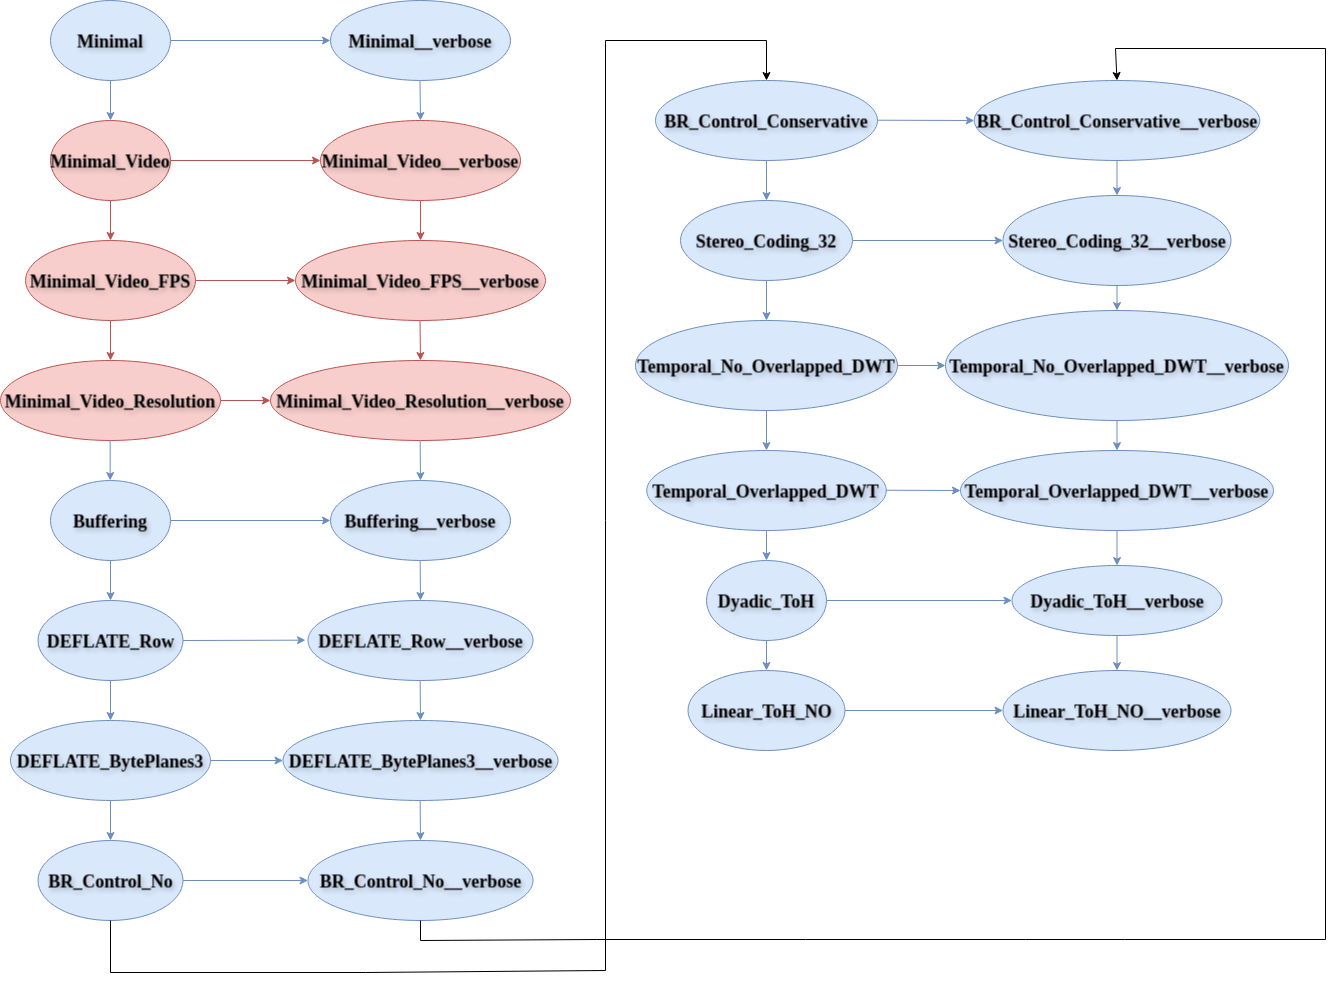
\includegraphics[width = 1.01\textwidth]{images/jerarquia_modulos.png}
	\captionof{figure}{Estructura jeraquizada de \textit{InterCom}.}
	\label{fig:jeraquia}
\end{center}

\vspace{\baselineskip}
Como se puede observar en la figura, el sistema se compone de varios módulos, cada uno de los cuales desempeña un papel específico en la funcionalidad general del programa. El módulo base o padre es \textit{Minimal} cuya función es la transmisión sin compresión, sin cuantificación, sin transformación, simplemente una transmisión bidireccional (\textit{full-duplex}) de trozos (\textit{chunks}) sin procesar y que sean reproducibles. De este módulo, parten todos los demás módulos que componen \textit{InterCom}, incluyedo los nuevos implementados. 
\vspace{\baselineskip}

Por mencionar algunos de los módulos que se pueden observar en la Figura \ref{fig:jeraquia} y su funcionamiento, por ejemplo, el módulo \textit{Buffering.py} implementa una estructura de búfer de acceso aleatorio para ocultar el jitter\footnote{El jitter simplemente es la fluctuación a la variabilidad temporal durante el envío de señales digitales, una ligera desviación de la exactitud de la señal de reloj. El jitter suele considerarse como una señal de ruido no deseada.}. Otro módulo que puede ser digno de mención es \textit{DEFLATE\_raw.py}, que implementa el algoritmo de compresión DEFLATE\footnote{El algoritmo DEFLATE se usa para la compresión de datos sin pérdidas que usa una combinación del algoritmo LZ77 y la codificación Huffman.} para comprimir cada trozo (chunk).

\vspace{\baselineskip}
En nuestro caso, nos centraremos en el módulo \textit{Minimal\_Video} y su version \textit{verbose}\footnote{La versión verbose simplemente muestra al ejecutar, estadísticas y datos adicionales a la versión normal.}, que son los que estan resaltados en la figura, así como, los módulos \textit{Minimal\_Video\_FPS} y \textit{Minimal\_Video\_Resolution} y sus versiones \textit{verbose} correspondiente, que son los que se han implementado y desarrollado en este trabajo.

\vspace{\baselineskip}
Como hemos comentado, el módulo \textit{Minimal\_Video} es el encargado de la transmisión de vídeo y audio en tiempo real. Este módulo se basa en el módulo \textit{Minimal} y añade la funcionalidad de captura, transmisión y recepción de vídeo, permitiendo una comunicación multimedia más completa. La versión \textit{verbose} proporciona información adicional sobre el rendimiento del sistema durante la ejecución. \textit{Minimal\_Video} será nuestro módulo base para los otros dos módulos adicionalmente implementados y desarrollados en este trabajo \textit{Minimal\_Video\_FPS} y \textit{Minimal\_Video\_Resolution}. En la siguiente Tabla \ref{tab:modulos} se muestra una comparativa resumida de que hace cada módulo implementado asi como de quien hereda, información sobre su versión \textit{verbose} y posibles casos de uso.

\begin{center}
\begin{tabular}{|p{2.6cm}|p{2.8cm}|p{3.7cm}|p{5cm}|}
    \cline{2-4} % Solo dibuja línea horizontal en columnas 2-4
    \multicolumn{1}{c|}{} & % Primera celda sin línea izquierda ni texto
    \textbf{Minimal\_Video} & 
    \textbf{Minimal\_Video\_FPS} & 
    \textbf{Minimal\_Video\_Resolution} \\
    \hline
    \textbf{Funcionalidad principal} & 
    Transmisión de vídeo y audio en tiempo real & 
    Ajuste de FPS según la resolución & 
    Configuración y reescalado a una resolución compatible \\
    \hline
    \textbf{Hereda de} & 
    Minimal & 
    Minimal\_Video & 
    Minimal\_Video\_FPS \\
    \hline
    \textbf{Versión verbose} & 
    Muestra estadísticas de rendimiento en tiempo real & 
    Incluye información sobre el ajuste de FPS realizado & 
    Muestra datos sobre el reescalado, la resolución y compatibilidad \\
    \hline

    \textbf{Caso de uso} & 
    Comunicación multimedia básica & 
    Cuando se requiere control específico de Cuadros por Segundo (\textit{FPS}) & 
    Cuando la resolución solicitada por el usuario no es compatible \\
    \hline
\end{tabular}
\captionof{table}{Comparativa de módulos implementados.}
\label{tab:modulos}
\end{center}
\vspace{\baselineskip}

\subsection{Cronología del proyecto}
El desarrollo de este proyecto se puede representar graficamente en un Diagrama de Gantt para poder conocer mejor los tiempos que se han requerido en hacer las distintas etapas y fases más importantes del mismo. Los hitos más relevantes del proyecto son:
\begin{itemize}
    \item \textbf{Selección tutor y proyecto:} En este primer \textit{milestone} (hito) se escogió al tutor basándose en la experiencia personal con el mismo en la asignatura de Tecnologías Multimedia así como, se le preguntó que tipo de trabajo se podría realizar. Como se ha comentado anteriormente, ya que en la asignatura se trabajó sobre el programa \textit{InterCom}, se decidió continuar con el mismo proyecto y desarrollarlo más en profundidad.
    \item \textbf{Entrega del anteproyecto:} Durante esta etapa, se redactó y entregó el documento del anteproyecto, el cual incluye la explicación y justificación del proyecto. 
    \item \textbf{Finalización de la implementación del código:} Esta fase abarca el desarrollo del código fuente de los módulos implementados en este proyecto, así como, la revisión por parte del profesor del mismo para asegurar su correcto funcionamiento según sus requerimientos y especificaciones.
    \item \textbf{Entrega del proyecto:} Por último, esta fase incluye la finalización de la redacción de la memoria del proyecto y finalmente su entrega, donde se documentan todo los puntos que se está actualmente viendo en este propio documento.
\end{itemize}

\vspace{\baselineskip}
\vspace{\baselineskip}
\vspace{\baselineskip}
\vspace{\baselineskip}

A continuación, en la Figura \ref{fig:planb} se puede observar el Diagrama de Gantt que representa la planificación del proyecto, incluyendo los hitos y las tareas principales. En este diagrama, se pueden observar tanto los tiempos estimados como los tiempos reales que han requerido cada una de las fases del proyecto.
\begin{figure}[H]
\centering
\begin{ganttchart}[
    hgrid,
    vgrid={*6{draw=none},dotted},
    x unit=0.371mm,
    y unit title=0.6cm,
    y unit chart=0.8cm,
    canvas/.style={draw=none},
    title/.append style={rounded corners=0.5mm},
    time slot format=isodate,
    time slot format/base century=2000,
    time slot unit=day,
    time slot format/start date=2024-09-01,
    bar height=0.45,
    bar label node/.append style={left=0.01cm, align=left, text width=11em},
    bar label text={#1},
    bar label font=\sffamily\footnotesize,
    group label node/.append style={left=0.01cm, align=left, text width=11em},
    group peaks width={3},
    group label font=\bfseries\footnotesize,
    milestone label font=\scshape\sffamily\footnotesize,
    milestone inline label node/.append style={left=5mm},
    milestone right shift=2,
    milestone left shift=-2,
    milestone/.append style={fill=black!40},
    title label font=\footnotesize\bfseries
]{2024-09-01}{2025-06-30}
    % Títulos de años y meses
    \gantttitle[title/.append style={fill=gray!10}]{2024}{122}
    \gantttitle[title/.append style={fill=gray!10}]{2025}{181} \\
    % Meses individuales
    \gantttitle{Sep}{30}
    \gantttitle{Oct}{31}
    \gantttitle{Nov}{30}
    \gantttitle{Dec}{31}
    \gantttitle{Jan}{31}
    \gantttitle{Feb}{28}
    \gantttitle{Mar}{31}
    \gantttitle{Apr}{30}
    \gantttitle{May}{31}
    \gantttitle{Jun}{30} \\
    % Tarea 0: Selección tutor y proyecto
    \ganttmilestone{Selección tutor y proyecto}{2024-09-01} \\
    % Tarea 1: Estudio InterCom
    \ganttgroup{\textbf{Análisis del código existente en Intercom}}{2024-09-02}{2024-09-10} \\
    \ganttbar[bar/.style={fill=blue!70}]{Estimado}{2024-09-02}{2024-09-10} \\
    \ganttbar[bar/.style={fill=red!70}]{Real}{2024-09-02}{2024-09-10} \\
    \ganttgroup{\textbf{Análisis de bibliotecas de captura de imágenes y vídeo}}{2024-09-10}{2024-09-12} \\
    \ganttbar[bar/.style={fill=blue!70}]{Estimado}{2024-09-10}{2024-09-12} \\
    \ganttbar[bar/.style={fill=red!70}]{Real}{2024-09-10}{2024-09-12} \\
    \ganttgroup{\textbf{Análisis de la biblioteca de transmisión de datos}}{2024-09-12}{2024-09-17} \\
    \ganttbar[bar/.style={fill=blue!70}]{Estimado}{2024-09-12}{2024-09-17} \\
    \ganttbar[bar/.style={fill=red!70}]{Real}{2024-09-12}{2024-09-17} \\
    \ganttmilestone{Estudio InterCom}{2024-09-17} \\
    % Tarea 2: Anteproyecto
    \ganttgroup{\textbf{Realización anteproyecto}}{2024-09-18}{2024-09-20} \\
    \ganttbar[bar/.style={fill=blue!70}]{Estimado}{2024-09-18}{2024-09-20} \\
    \ganttbar[bar/.style={fill=red!70}]{Real}{2024-09-18}{2024-09-20} \\
    \ganttmilestone{Entrega anteproyecto}{2024-09-20} \\
    % Tarea 3: Implementación
    \ganttgroup{\textbf{Implementación del código}}{2024-10-15}{2025-05-08} \\
    \ganttbar[bar/.style={fill=blue!70}]{Estimado}{2024-10-15}{2025-04-30} \\
    \ganttbar[bar/.style={fill=red!70}]{Real}{2024-11-11}{2025-05-08} \\
    \ganttmilestone{Finalización implementación}{2025-05-08} \\
    % Tarea 4: Memoria
    \ganttgroup{\textbf{Realización memoria proyecto}}{2025-05-01}{2025-05-24} \\
    \ganttbar[bar/.style={fill=blue!70}]{Estimado}{2025-05-01}{2025-05-20} \\
    \ganttbar[bar/.style={fill=red!70}]{Real}{2025-05-09}{2025-05-24} \\
    \ganttmilestone{Entrega proyecto}{2025-05-31} \\
\end{ganttchart}
\caption{Planificación del proyecto sobre LaTeX con tiempos estimados y reales.}
\label{fig:planb}
\end{figure}
\vspace{\baselineskip}

Como se puede observar en el diagrama, el proyecto comenzó aproximadamente el día \textbf{1 de septiembre} en el que, el tutor y yo, habíamos ya acordado previamente, antes del comienzo del curso académico, cuál iba a ser el proyecto a realizar.
\vspace{\baselineskip}

A partir de ahí, se procedió a analizar el código ya existente en \textit{InterCom}, que ya se había observado y parcialmente analizado de antemano en la asignatura de \textit{Tecnologías Multimedia}, por lo que no se dispensó de mucho tiempo en esta parte del trabajo. Además, las bibliotecas relacionadas con la captura y visualización del vídeo como \textit{opencv-python} fueron rápidas de analizar y relativamente sencillas de comprender, por lo que para el \textbf{12 de septiembre} esta parte estaría ya completada. Las demás bibliotecas necesarias para la envío y recepción de los datos, resultaron intuitivas y relativamente fáciles de usar por lo que no ocupó mucho tiempo en estudiar sus distintas funciones y métodos, lo que lleva a que se terminase el estudio del \textit{InterCom} y las distintas bibliotecas en torno al \textbf{17 de septimebre}. 
\vspace{\baselineskip}

Seguidamente, se realizó el anteproyecto que fue rápido de redactar y se entregó el \textbf{20 de septiembre} y justamente después, se comenzó con la implementación del código que fue la fase más larga del proyecto y que se finalizó el \textbf{8 de mayo}. 
\vspace{\baselineskip}

Por último, se realizará la entrega de esta memoria del proyecto, a priori, para aproximadamente el \textbf{31 de mayo}. Como se puede observar, los tiempos reales han sido superiores a los estimados en la mayoría de los casos sobre todo en la implementación del código ya que hubo que realizar distintas pruebas para que los módulos implementados en este trabajo estuvieran correctamente integrados con los demás que ya había previamente en \textit{InterCom}, así como, la posterior optimización de los mismos que es la última etapa de la implementación, lo cual es normal en este tipo de proyectos.

\vspace{\baselineskip}
Con esto acaba el capítulo de \textit{Introducción}. En el siguiente capítulo, se presentará la metodología utilizada para el desarrollo del proyecto, incluyendo los pasos seguidos y las herramientas empleadas así como, la explicación completa del código desarrollado. 

\newpage
\section{Metodología}
{\color{tfgazul}\rule{\textwidth}{3pt}}
\label{sec:metodologia}

\subsection{Especificaciones técnicas del proyecto}

Antes de pasar a explicar el codigo implementado, es importante mencionar las especificaciones técnicas del proyecto así como algunos requerimientos técnicos para tener un mejor entendimiento del programa implementado y su uso. 
\vspace{\baselineskip}

El proyecto se ha desarrollado en un entorno virtual, a través del software de virtualización \textit{Oracle VirtualBox}\footnote{https://www.virtualbox.org/}, en el cual se ha instalado el sistema operativo \textit{Xubuntu}\footnote{https://xubuntu.org/} que es una distribución Linux basada en Ubuntu. El lenguaje de programación, usado ya en \textit{InterCom} y que se ha usado tambien para seguir desarrollándolo con los nuevos módulos implementados en este trabajo, es Python. 
\vspace{\baselineskip}

\begin{center}
	
\includegraphics[width = 0.32\textwidth]{images/oracle_xubuntu.png}
	\captionof{figure}{Logo de Oracle VirtualBox y Xubuntu}
	\label{fig:oraclexubuntu}
\end{center}

\vspace{\baselineskip}

Hay que tener en cuenta que para el correcto funcionamiento de \textit{InterCom} así como de los módulos desarrollados en este trabajo, hay que instalar diversos paquetes y hacer uso de librerías concretas que se detallan a continuación. A continuación, se muestra en la tabla \ref{tab:paquetes} la lista de paquetes y librerías necesarias para el correcto funcionamiento del sistema \textit{InterCom} y de los módulos implementados en este trabajo:

\begin{center}
\captionof{table}{Paquetes y librerias utilizadas}
\label{tab:paquetes}
\begin{tabular}{|p{2.5cm}|p{12.6cm}|}
    \hline
    \textbf{Paquete} & \textbf{Descripción } \\
    \hline
    argcomplete & Herramienta que proporciona el autocompletado en la linea de comandos, con la tecla TAB para aplicaciones Python que utilizan ``argparse''. \\
    \hline
    pywavelets & Biblioteca de Python para el análisis de señales y procesamiento de imágenes mediante transformadas wavelet (ondículas). \\
    \hline
    sounddevice & Biblioteca que permite grabar y reproducir audio en tiempo real a través de la tarjeta de sonido del sistema. \\
    \hline
    soundfile & Lectura y escritura de la mayoría de formatos de archivo de sonido. \\
    \hline
    matplotlib & Creación de gráficos y visualizaciones estáticas/interactivas. \\
    \hline
    scipy & Biblioteca fundamental para la computación científica y técnica. \\
    \hline
    spectrum & Biblioteca que sirve para calcular y visualizar el espectro de frecuencias de una señal digital. \\
    \hline
    numpy & Soporte para arrays y matrices multidimensionales grandes. \\
    \hline
    psutil & Información del sistema y monitorización de procesos. \\
    \hline
    opencv-python & Biblioteca para la visualización del vídeo en tiempo real. \\
    \hline
    pygame & Conjunto de módulos Python para el desarrollo de videojuegos y aplicaciones multimedia. \\
    \hline
    pygame\_widgets & Proporciona widgets listos para usar en aplicaciones y juegos desarrollados con pygame. \\
    \hline
    setuptools & Biblioteca y conjunto de herramientas para facilitar la creación, empaquetado, distribución e instalación de proyectos Python. \\
    \hline
\end{tabular}
\end{center}

\subsection{Código implementado}
En esta sección, se procederá a comentar, prácticamente, línea por línea o en su defecto bloques de código similares, para mayor entendimiento del mismo. A su vez, cada módulo se dividirá en dos subsecciones para explicar tanto la versión normal del código como la ``verbose''. El código completo implementado en este trabajo se encuentra disponible en el repositorio de GitHub \url{https://github.com/JJsanriv/TFG-Intercom-Video}.

\subsubsection{Codigo del módulo Minimal\_Video.py}

En primer lugar, se comenzará por explicar el código del módulo \textit{minimal\_video.py} que es el módulo base que se encarga de la captura, transmisión, recepción y visualización del video. Los otros dos módulos que se han desarrollado en este trabajo parten de este, por lo que, muchos métodos y la estructura son muy similares y se sigue la misma lógica en todos ellos. A su vez, este módulo parte de la base que hay en \textit{minimal.py} implementada en \textit{InterCom}. El código de este módulo es el siguiente:
\begin{lstlisting}[style=pythonstyle, caption={Comienzo del módulo \textit{minimal\_video.py} y sus parámetros}, label={lst:principio_clase_minimal}]
#!/usr/bin/env python
# PYTHON_ARGCOMPLETE_OK

import cv2
import socket
import struct
import threading
import time
import math
import numpy as np
import select
import argparse
import psutil
import minimal

spinner = minimal.spinning_cursor()

def int_or_str(text):
    try:
        return int(text)
    except ValueError:
        return text

if not hasattr(minimal, 'parser'):
    minimal.parser = argparse.ArgumentParser(formatter_class=argparse.ArgumentDefaultsHelpFormatter)
parser = minimal.parser

parser.add_argument("-v", "--video_payload_size", type=int, default=1400, help="Tamano deseado (bytes) payload video/fragmento UDP (defecto 1400).")
parser.add_argument("-w", "--width", type=int, default=320, help="Ancho video (defecto 320)")
parser.add_argument("-g", "--height", type=int, default=240, help="Alto video (defecto 240)")
parser.add_argument("-z", "--fps", type=int, default=30, help="Frames por segundo video (defecto 30)")
parser.add_argument("--show_video", action="store_true", default=False, help="Habilita la visualizacion y transmision del video (desactivado por defecto).")
parser.add_argument("--video_port", type=int, default=4445, help="Puerto para transmitir/recibir video (defecto 4445).")

args = None
\end{lstlisting}

A continuación, se encuentra la explicación del bloque de código \ref{lst:principio_clase_minimal}:

\begin{itemize}
    \item \textbf{Línea 1:} se define el ``shebang'' que indica que el script debe ejecutarse con Python.
    \item \textbf{Línea 2:} se indica que el script es compatible con la autocompletación de argumentos en la línea de comandos.
    \item \textbf{Líneas 4-14:} se importan las librerías necesarias para el funcionamiento del módulo. Estas librerías son fundamentales para la captura, transmisión y recepción de video, así como para la manipulación de datos y la creación de sockets.
    \item \textbf{Línea 16:} se define el objeto \textit{spinner} que se usará para mostrar un cursor giratorio en la línea de comandos mientras se espera la entrada del usuario.
    \item \textbf{Líneas 18-22:} se define la función \textit{int\_or\_str()} que intenta convertir un texto en un entero. Si no puede, devuelve el texto original. Esta función se usará para procesar argumentos de línea de comandos.
    \item \textbf{Líneas 24-26:} se verifica si el módulo \textit{minimal} tiene un atributo llamado \textit{parser}. Si no lo tiene, se crea un nuevo objeto \textit{ArgumentParser} para procesar los argumentos de línea de comandos. Este objeto se usará para definir y gestionar los argumentos que se pasan al script.
    \item \textbf{Línea 28-33:} se definen varios argumentos de línea de comandos que se pueden usar al ejecutar el script. Estos argumentos permiten al usuario personalizar el comportamiento del programa, como el tamaño del payload de video, las dimensiones del video, los frames por segundo, la habilitación de la visualización del video y el puerto para la transmisión y recepción de video.
    \item \textbf{Línea 35:} se inicializa la variable \textit{args} como \textit{None}. Esta variable se usará para almacenar los argumentos procesados por el parser.
\end{itemize}

\vspace{\baselineskip}

Ahora, se procede a explicar el comienzo de la clase \textit{Minimal\_Video} y parte del metodo \textit{\_init\_} que es el que se encarga de inicializar la clase y sus atributos. El código es el siguiente:

\begin{lstlisting}[style=pythonstyle, caption={Comienzo de la clase \textit{Minimal\_Video} y parte de la inicialización}, label={lst:inicializacion_minimal_video}]
class Minimal_Video(minimal.Minimal):
    def __init__(self):
        global args
        if args is None:
            args = minimal.parser.parse_args()
        minimal.args = args

        super().__init__()

        if not args.show_video:
            return

        self.video_sock = socket.socket(socket.AF_INET, socket.SOCK_DGRAM)
        self.video_sock.setsockopt(socket.SOL_SOCKET, socket.SO_REUSEADDR, 1)
        self.video_sock.setsockopt(socket.SOL_SOCKET, socket.SO_RCVBUF, 8388608)
        self.video_sock.setsockopt(socket.SOL_SOCKET, socket.SO_SNDBUF, 8388608)
        self.video_sock.setblocking(False)
        try:
            self.video_sock.bind(("0.0.0.0", args.video_port))
        except OSError as e:
            print(f"Error bind socket video: {e}")
            raise
        self.video_addr = (args.destination_address, args.video_port)

        self._header_format = "!H"
        self.header_size = 2
        self.effective_video_payload_size = args.video_payload_size
        self.max_payload_possible = self.effective_video_payload_size - self.header_size
        self.effective_video_payload_size = max(1, min(args.video_payload_size, self.max_payload_possible))
        if self.effective_video_payload_size != args.video_payload_size:
            print(f"Aviso: --video_payload_size ajustado a {self.effective_video_payload_size} bytes.")

        self.cap = None
        self.width = 0
        self.height = 0
        self.fps = 0

        self.expected_frame_size = 0
        self.total_frags = 0
\end{lstlisting}

A continuación, se encuentra la explicación del bloque de código \ref{lst:inicializacion_minimal_video}:

\begin{itemize}
    \item \textbf{Línea 1:} se define la clase \textit{Minimal\_Video} que hereda de la clase \textit{Minimal} del módulo \textit{minimal.py}.
    \item \textbf{Línea 2:} se define el método \textit{\_\_init\_\_} que es el constructor de la clase.
    \item \textbf{Líneas 3-6:} se inicializa la variable \textit{args} con los argumentos procesados por el parser. Si \textit{args} ya tiene un valor, se omite esta parte.
    \item \textbf{Línea 8:} se llama al constructor de la clase padre \textit{Minimal} para inicializar sus atributos.
    \item \textbf{Líneas 10-11:} se verifica si la opción de mostrar video está habilitada. Si no lo está, se sale del método ya que no necesitariamos inicializar todas las variables y métodos correspondientes con el vídeo.
    \item \textbf{Línea 13:} se crea un socket UDP para la transmisión de video. socket.AF\_INET indica que se usará IPv4 y socket.SOCK\_DGRAM indica que se usará UDP.
    \item \textbf{Líneas 14-16:} se configuran opciones del socket para permitir la reutilización de la dirección IP y puertos usados\footnote{La reutilización de la dirección sirve para que no nos muestre el error ``Address already in use'' al ejecutar el programa varias veces seguidas.} y aumentar el tamaño del buffer de recepción y envío a 8MB\footnote{Permite mayor flexibilidad al manejar mayor cantidad de datos de vídeo sin pérdidas cuando hay picos en la recepción.}.
    \item \textbf{Línea 17:} se establece el socket como no bloqueante, lo que significa que las operaciones de lectura y escritura no bloquearán el socket de video si no hay datos disponibles.\footnote{Permite que el programa continúe ejecutándose mientras maneja la comunicación de vídeo sin quedar bloqueado. Esencial para aplicaciones en tiempo real, en concreto la nuestra.}
    \item \textbf{Líneas 18-22:} se configura el socket para escuchar conexiones entrantes en todas las interfaces de red (dirección IP ``0.0.0.0'') en el puerto especificado por el argumento video\_port.\footnote{ Si la operación falla (por ejemplo, porque el puerto ya está en uso), captura el error OSError, muestra un mensaje descriptivo y lanza la excepción para terminar la ejecución del programa.}
    \item \textbf{Línea 23:} se inicializa la variable \textit{video\_addr} con la dirección IP de destino y el puerto de video.
    \item \textbf{Línea 25-26:} se define el formato del encabezado del paquete de video como un entero sin signo de 16 bits (2 bytes) usando el formato de la librería struct. 
    \item \textbf{Líneas 27-31:} Primero asigna el valor proporcionado por el usuario (\textit{args.video\_payload\_size}) a \textit{self.effective\_video\_payload\_size}. Luego, se calcula el máximo payload posible restando el tamaño de la cabecera (\textit{self.header\_size}) del tamaño deseado. Procede a ajustar \textit{self.effective\_video\_payload\_size} para que esté entre 1 y el máximo payload posible calculado. Por ultimo, si el valor final es diferente del solicitado por el usuario, muestra un mensaje de aviso indicando que se ha ajustado automáticamente.\footnote{Este trozo de código garantiza que el tamaño del payload sea válido para la transmisión de video, evitando valores demasiado pequeños o muy grandes que superen el límite permitido por el tamaño de la cabecera.}
    \item \textbf{Líneas 33-36:} se inicializan varias variables relacionadas con la captura de video. \textit{self.cap} se usará para almacenar el objeto de captura de video, \textit{self.width} y \textit{self.height} almacenan las dimensiones del video, \textit{self.fps} almacena los frames por segundo.
    \item \textbf{Líneas 38-39:} se inicializan las variables \textit{self.expected\_frame\_size} y \textit{self.total\_frags} que se usarán para almacenar el tamaño esperado de un fotograma y el número total de fragmentos del video.
\end{itemize}

\vspace{\baselineskip}

Terminamos la funcion \textit{\_init\_} de la forma que se observa en el bloque de código \ref{lst:fin_ini_minimal_video}
\vspace{\baselineskip}
\begin{lstlisting}[style=pythonstyle, caption={Fin de la inicialización de Minimal\_Video}, label={lst:fin_ini_minimal_video}]
print("Flag --show_video detectado. Intentando inicializar la camara...")
        try:
            self.cap = cv2.VideoCapture(0)
            if not self.cap.isOpened():
                raise IOError("No se pudo abrir la camara.")
            if args.width > 0:
                self.cap.set(cv2.CAP_PROP_FRAME_WIDTH, args.width)
            if args.height > 0:
                self.cap.set(cv2.CAP_PROP_FRAME_HEIGHT, args.height)
            if args.fps > 0:
                self.cap.set(cv2.CAP_PROP_FPS, args.fps)
            self.cap.set(cv2.CAP_PROP_BUFFERSIZE, 2)
            self.width = int(self.cap.get(cv2.CAP_PROP_FRAME_WIDTH))
            self.height = int(self.cap.get(cv2.CAP_PROP_FRAME_HEIGHT))
            self.fps = int(self.cap.get(cv2.CAP_PROP_FPS))

            self.expected_frame_size = self.width * self.height * 3
            self.total_frags = math.ceil(self.expected_frame_size / self.effective_video_payload_size)

            self.fragment_ranges = []
            self.fragment_headers = []
            for frag_idx in range(self.total_frags):
                start = frag_idx * self.effective_video_payload_size
                end = min(start + self.effective_video_payload_size, self.expected_frame_size)
                self.fragment_ranges.append((start, end))
                self.fragment_headers.append(struct.pack(self._header_format, frag_idx))

            self.remote_frame = np.zeros((self.height, self.width, 3), dtype=np.uint8)
            
        except Exception as e:
            print(f"Error al inicializar la camara: {e}. Deshabilitando video.")
            if self.cap:
                self.cap.release()
            self.cap = None

        self.running = True
\end{lstlisting}

\begin{itemize}
    \item \textbf{Línea 1:} se imprime un mensaje indicando que se ha detectado la opción \textit{--show\_video} y que se intentará inicializar la cámara.\footnote{Evidentemente el usaurio tiene que tener la cámara conectada y activada.}
    \item \textbf{Líneas 2-5:} se intenta inicializar la cámara usando \textit{cv2.VideoCapture(0)}. Si no se puede abrir, lanza una excepción con un mensaje de error.
    \item \textbf{Líneas 6-11:} se configuran las propiedades de la cámara (ancho, alto y FPS) según los argumentos proporcionados por el usuario. Si los valores son mayores que 0, se aplican.
    \item \textbf{Línea 12:} se establece el tamaño del buffer de la cámara a 2 fotogramas, lo que ayuda a reducir la latencia en la captura de video.\footnote{El tamaño del buffer se refiere a la cantidad de fotogramas que se almacenan temporalmente antes de ser procesados. Un tamaño de buffer más pequeño puede reducir la latencia, pero también puede aumentar el riesgo de pérdida de fotogramas si la cámara no puede enviar datos lo suficientemente rápido.}
    \item \textbf{Líneas 13-15:} se obtienen las dimensiones del video (ancho, alto y FPS) y se almacenan en las variables correspondientes.
    \item \textbf{Líneas 17-18:} se calcula el tamaño esperado de un fotograma (en bytes) multiplicando el ancho, la altura y 3 (3 bytes por píxel para un video RGB) y se almacena en \textit{self.expected\_frame\_size}. Luego, se calcula el número total de fragmentos necesarios para enviar el fotograma completo dividiendo el tamaño esperado por el tamaño efectivo del payload de video.
    \item \textbf{Líneas 20-21:} se inicializan dos listas vacías: \textit{self.fragment\_ranges} y \textit{self.fragment\_headers}. Estas listas se usarán para almacenar los rangos de fragmentos y los encabezados de cada fragmento.
    \item \textbf{Líneas 22-26:} se itera sobre el número total de fragmentos y se calcula el rango de bytes para cada fragmento. Se empaqueta el índice del fragmento en un encabezado usando \textit{struct.pack} y se añaden a las listas correspondientes. Esto sirve para dividir el fotograma en fragmentos que se enviarán por separado a través de la red.
    \item \textbf{Línea 28:} esta línea crea un \textit{frame} inicializado en negro (todos los valores en 0) para que sea el primer frame que se muestre y a partir de ahí que se actualicen con los frames reales.
    \item \textbf{Líneas 30-34:} este bloque de código garantiza que si ocurre un error al inicializar la cámara, se capture la excepción y se liberen los recursos utilizados así, el programa puede continuar ejecutándose sin intentar usar el vídeo. Es una medida de seguridad y limpieza de recursos contra posible fallos del programa.
    \item \textbf{Línea 36:} esta variable indica cuando la instancia de la clase está en ejecución y permite controlar el ciclo principal del procesamiento de vídeo y su transmisión. Cuando se termina la ejecución del programa, se establece a ``false'' para que paren todos los procesos relacionados con el vídeo.
\end{itemize}

Ahora, una vez terminada la incialización de la clase \textit{Minimal\_Video}, procedemos a explicar cada método que se usa para la captura, transmisión, recepción y captura de vídeo así como el metodo para ejecutar de forma correcta y adecuada estos mismos.
\vspace{\baselineskip}

Comenzamos con el método \textit{capture\_image()} que se puede observar en el bloque de código \ref{lst:capture_frame}, el cual realiza la captura de vídeo:
\begin{lstlisting}[style=pythonstyle, caption={Método capture\_frame() de \textit{Minimal\_Video}}, label={lst:capture_frame}]
def capture_image(self):
        _, frame = self.cap.read()
        return frame.tobytes()
\end{lstlisting}

\begin{itemize}
    \item \textbf{Línea 1:} se define el método \textit{capture\_image()} que no toma argumentos.
    \item \textbf{Línea 2:} se usa el método \textit{read()} de opencv-python para capturar un fotograma de video. Este método devuelve dos valores: \textit{ret} un valor booleano que indica si la captura fue exitosa (Usamos ``\_'' ya que no lo necesitamos) y \textit{frame} (el fotograma capturado).
    \item \textbf{Línea 3:} si la captura es correcta, se convierte el fotograma a bytes usando el método \textit{tobytes()} y se devuelve. Este método convierte la imagen capturada en un formato de bytes que se puede enviar a través de la red.
\end{itemize}
\vspace{\baselineskip}

El siguiente bloque de código \ref{lst:send_fragment} se encargará de enviar los fragmentos de video a través del socket de vídeo UDP:
\begin{lstlisting}[style=pythonstyle, caption={Método send\_video\_fragment() de \textit{Minimal\_Video}}, label={lst:send_fragment}]
def send_video_fragment(self, frag_idx, data):
        start, end = self.fragment_ranges[frag_idx]
        payload = data[start:end]
        packet = self.fragment_headers[frag_idx] + payload
        try:
            self.video_sock.sendto(packet, self.video_addr)
        except BlockingIOError:
            print(f"Socket bloqueado al enviar fragmento {frag_idx}.")
            pass
        return len(packet)
\end{lstlisting}

\begin{itemize}
    \item \textbf{Línea 1:} se define el método \textit{send\_video\_fragment} que toma como argumentos el índice del fragmento (\textit{frag\_idx}) y los datos del fotograma (\textit{data}).
    \item \textbf{Línea 2:} se obtienen los rangos de inicio y fin del fragmento correspondiente al índice proporcionado.
    \item \textbf{Línea 3:} se extraen los datos del fotograma en el rango especificado y se almacenan en la variable \textit{payload}.
    \item \textbf{Línea 4:} se crea el paquete concatenando el encabezado del fragmento y los datos del fotograma.
    \item \textbf{Líneas 5-9:} se intenta enviar el paquete a través del socket de vídeo UDP usando el método \textit{sendto()}. Si el socket está bloqueado, se captura la excepción \textit{BlockingIOError} y se imprime un mensaje de advertencia. En este caso, simplemente se pasa y no se hace nada.\footnote{Aunque el socket se estableció como no bloqueante, puede haber ocasiones en las que el socket esté temporalmente bloqueado debido a la congestión de la red o a otros factores.}
    \item \textbf{Línea 10:} se devuelve la longitud del paquete enviado, que será util en módulos derivados de este.\footnote{Se verá más adelante en el módulo \textit{Minimal\_Video\_FPS} que se usa para calcular el tamaño del paquete enviado.}
\end{itemize}
\vspace{\baselineskip}

En el siguiente bloque de código \ref{lst:receive_fragment} se encuentra el método que se encarga de recibir los fragmentos de video a través del socket de vídeo UDP:
\begin{lstlisting}[style=pythonstyle, caption={Método receive\_video\_fragment() de \textit{Minimal\_Video}}, label={lst:receive_fragment}]
def receive_video_fragment(self):
        rlist, _, _ = select.select([self.video_sock], [], [], 0.001)
        if rlist:
            packet, addr = self.video_sock.recvfrom(self.effective_video_payload_size + self.header_size)
            header = packet[:self.header_size]
            payload = packet[self.header_size:]
            recv_frag_idx, = struct.unpack(self._header_format, header)
            start = recv_frag_idx * self.effective_video_payload_size
            end = min(start + len(payload), self.expected_frame_size)
            flat_frame = self.remote_frame.reshape(-1) # Flatten the frame for direct assignment
            flat_frame[start:end] = np.frombuffer(payload, dtype=np.uint8, count=(end - start)) # Direct assignment
            return recv_frag_idx, len(packet)
        return None, 0
\end{lstlisting}

A continuación, se explican las líneas de código que se muestran en el bloque de código \ref{lst:receive_fragment}:
\begin{itemize}
    \item \textbf{Línea 1:} se define el método \textit{receive\_video\_fragment} que no toma argumentos.
    \item \textbf{Línea 2:} se usa la función \textit{select.select()} para esperar a que haya datos disponibles en el socket de video. Esta función permite ver cuando el socket de vídeo esta libre para recibir el fragmento. En este caso, se espera un máximo de 1 milisegundos.\footnote{Ajustar el tiempo de espera a 1 ms ha sido la configuración más óptima encontrada}
    \item \textbf{Línea 3:} si hay datos disponibles (rlist no está vacío), se entra en la condición.
    \item \textbf{Línea 4:} se recibe el paquete de datos del socket usando el método \textit{recvfrom()}\footnote{El método recvfrom internamente realiza las siguientes operaciones: bloquea la ejecución hasta recibir datos en el socket de vídeo UDP, captura los bytes entrantes según el tamaño especificado (effective\_video\_payload\_size + header\_size), identifica la dirección IP y puerto del remitente, y devuelve tanto los datos recibidos como la información del remitente como una tupla (paquete, dirección).}. Este método devuelve el paquete recibido y la dirección del remitente. El tamaño máximo del paquete es el tamaño efectivo del payload más el tamaño del encabezado.
    \item \textbf{Línea 5:} se extrae el encabezado del paquete recibido.
    \item \textbf{Líneas 6:} se extraen los datos del payload del paquete recibido, omitiendo el encabezado.
    \item \textbf{Línea 7:} se desempaqueta el encabezado para obtener el índice del fragmento recibido usando la función \textit{struct.unpack()}.\footnote{La función struct.unpack() convierte los bytes del encabezado en un entero, que representa el índice del fragmento recibido.}
    \item \textbf{Línea 8:} se define la varible \textit{start} que representa el inicio del rango de bytes del fragmento recibido.
    \item \textbf{Línea 9:} se define la variable \textit{end} que representa el final del rango de bytes del fragmento recibido. Se asegura de que no exceda el tamaño esperado del fotograma.
    \item \textbf{Línea 10:} se aplana el fotograma remoto para facilitar la asignación directa de los datos del payload. Esto convierte el fotograma en un array unidimensional, lo que permite acceder a los elementos de manera más sencilla.\footnote{El método reshape(-1) convierte el array multidimensional en un array unidimensional, manteniendo el mismo número total de elementos.}
    \item \textbf{Línea 11:} se asignan directamente los datos del payload al rango correspondiente en el fotograma remoto usando la función np.frombuffer() para convertir los bytes en un array NumPy. Esto permite que los datos del payload se copien directamente en el fotograma remoto en la posición correcta.\footnote{La función np.frombuffer() crea un array NumPy a partir de un buffer de bytes, permitiendo especificar el tipo de dato y la cantidad de elementos a leer.}
    \item \textbf{Línea 12:} se devuelve el índice del fragmento recibido y la longitud del paquete recibido.
    \item \textbf{Línea 13:} si no hay datos disponibles, se devuelve \textit{None} y 0.
\end{itemize}
\vspace{\baselineskip}

Seguidamente, continuamos explicando el método \textit{show\_video()} que es el que se encargará de mostrar el video en una ventana utilizando \textit{OpenCV}:
\begin{lstlisting}[style=pythonstyle, caption={Método show\_video() de \textit{Minimal\_Video}}, label={lst:show_video}]
    def show_video(self):
        cv2.imshow("Video", self.remote_frame)
        cv2.waitKey(1)
\end{lstlisting}

A continuación, se explican las líneas de código referentes al bloque de código \ref{lst:show_video}:
\begin{itemize}
    \item \textbf{Línea 1:} se define el método \textit{show\_video()} que no toma argumentos.
    \item \textbf{Línea 2:} se muestra el fotograma remoto en una ventana llamada ``Video'' usando la función \textit{cv2.imshow()} de OpenCV.
    \item \textbf{Línea 3:} se espera 1 milisegundo para permitir que la ventana se actualice y procese posibles pulsaciones del teclado usando la función \textit{cv2.waitKey()}.
\end{itemize}
\vspace{\baselineskip}

El siguiente método \textit{video\_loop()} es el más importante de la clase ya que es el bucle principal que captura, envía y recibe los fragmentos de vídeo usando los métodos anteriormente definidos. El código es el siguiente:
\begin{lstlisting}[style=pythonstyle, caption={Método video\_loop() de \textit{Minimal\_Video}}, label={lst:video_loop_minimal_video}]
def video_loop(self):
        try:
            while self.running:
                data = self.capture_image()
                for frag_idx in range(self.total_frags):
                    self.send_video_fragment(frag_idx, data)
                    self.receive_video_fragment()
                self.show_video()
        except Exception as e:
            print(f"Error en el bucle de video: {e}")
            pass
\end{lstlisting}

\vspace{\baselineskip}
A continuación, se explica el bloque de código \ref{lst:video_loop_minimal_video}:
\vspace{\baselineskip}
\begin{itemize}
    \item \textbf{Línea 1:} se define el método \textit{video\_loop()} que no toma argumentos.
    \item \textbf{Línea 2:} se usa un bloque try-except para manejar posibles excepciones durante la ejecución del bucle.
    \item \textbf{Línea 3:} se inicia un bucle while que continuará ejecutándose mientras la variable \textit{self.running} sea verdadera.
    \item \textbf{Línea 4:} se captura una imagen de video usando el método \textit{capture\_image()} y se almacena en la variable \textit{data}.
    \item \textbf{Línea 5:} se itera sobre el número total de fragmentos y se envía cada fragmento usando el método \textit{send\_video\_fragment()}.
    \item \textbf{Línea 6:} se recibe cada fragmento usando el método \textit{receive\_video\_fragment()}.
    \item \textbf{Línea 7:} se muestra el fotograma remoto en la ventana de video usando el método \textit{show\_video()}.
\end{itemize}

\vspace{\baselineskip}

Por ultimo, se mostrará el método \textit{run()} que es el que se encargará de ejecutar el bucle principal del programa y gestionar la lógica de ejecución del mismo:
\begin{lstlisting}[style=pythonstyle, caption={Método run() de \textit{Minimal\_Video}}, label={lst:run_minimal_video}]
def run(self):
        if not args.show_video or self.cap is None:
            print("Video desactivado. Ejecutando solo la parte de audio.")
            super().run()
            return

        print("Iniciando video con bucle unificado y protocolo simplificado...")

        t_unified = threading.Thread(target=self.video_loop, daemon=True, name="UnifiedVideoThread")
        t_unified.start()

        try:
            super().run()
        except KeyboardInterrupt:
            print("Interrupcion por teclado detectada.")
        finally:
            self.running = False
            if t_unified.is_alive():
                t_unified.join(timeout=1)
            if hasattr(self, 'cap') and self.cap.isOpened():
                self.cap.release()
            cv2.destroyAllWindows()
            if hasattr(self, 'video_sock') and self.video_sock:
                self.video_sock.close()
            print("Aplicacion de video detenida.")
\end{lstlisting}
\vspace{\baselineskip}
A continuación, se explican las líneas de código que se muestran en el bloque de código \ref{lst:run_minimal_video}:

\begin{itemize}
    \item \textbf{Línea 1:} se define el método \textit{run()} que no toma argumentos.
    \item \textbf{Líneas 2-5:} se verifica si la opción de mostrar video está habilitada y si la cámara está disponible. Si no lo están, se imprime un mensaje indicando que el video está desactivado y se llama al método \textit{run()} de la clase padre \textit{Minimal} para ejecutar solo la parte de audio.
    \item \textbf{Líneas 7:} si la cámara está disponible, se imprime un mensaje indicando que se iniciará el video con un bucle unificado y protocolo simplificado.
    \item \textbf{Líneas 9-10:} se crea un hilo (thread) para ejecutar el método \textit{video\_loop()} de forma paralela. Se establece como un hilo daemon, lo que significa que se cerrará automáticamente cuando el programa principal termine. Se inicia el hilo.
    \item \textbf{Líneas 12-15:} se intenta ejecutar el método \textit{run()} de la clase padre \textit{Minimal} para manejar la parte de audio. Si se detecta una interrupción por teclado (Ctrl+C), se captura la excepción \textit{KeyboardInterrupt} y se imprime un mensaje.
    \item \textbf{Líneas 16-25:} en el bloque finally, se establece \textit{self.running} a falso para detener el bucle de video. Si el hilo de video aún está vivo, se espera a que termine usando \textit{join()}. Luego, se liberan los recursos de la cámara y se cierran las ventanas de OpenCV. Finalmente, se cierra el socket de video y se imprime un mensaje indicando que la aplicación de video ha sido detenida.
\end{itemize}

\vspace{\baselineskip}

Ahora, se procede a explicar la versión ``verbose'' del módulo \textit{minimal\_video.py} que se encargará de hacer lo mismo que la versión normal ya que ejecuta los métodos de la clase padre pero añadiendo una serie de estadísitcas con respecto al vídeo, como monitorizar la cantidad de paquetes que se reciben y se envían, porcentaje de uso de la CPU y más. Para activar esta versión del código hay que usar alguna de los cuatro ``flags'' que lo activan, los cuales son ``--show\_stats'', ``--show\_samples'', ``--show\_spectrum'' y ``--reading\_time''. Las salidas de estos ``flags'' se mostrarán más adelante. 
\vspace{\baselineskip}

El código correspondiente al comienzo de esta parte del módulo es el siguiente:

\begin{lstlisting}[style=pythonstyle, caption={Código de la inicialización de Minimal\_Video\_verbose}, label={lst:verbose_minimal_video}]
class Minimal_Video__verbose(Minimal_Video, minimal.Minimal__verbose):
    def __init__(self):
        super().__init__()

        if not args.show_video or not hasattr(self, 'cap') or self.cap is None:
            return

        try:
            minimal.Minimal__verbose.__init__(self)
            print(f"Verbose Mode: stats cycle = {self.seconds_per_cycle}s")
        except AttributeError:
            print("Error: No se pudo inicializar minimal.Minimal__verbose. Las estadisticas no funcionaran.")

        self.video_sent_bytes_count = 0
        self.video_sent_messages_count = 0
        self.video_received_bytes_count = 0
        self.video_received_messages_count = 0

        self._total_audio_sent_bytes = 0
        self._total_audio_received_bytes = 0
        self._total_video_sent_bytes = 0
        self._total_video_received_bytes = 0
        self._stats_start_time = time.time()

        self._fragments_received_this_cycle = 0
        self._fragments_received_history = []

        self.total_number_of_sent_frames = 0
        self.frame_time = 1.0 / self.fps

        self.end_time = None
        if hasattr(args, "reading_time") and args.reading_time:
            self.end_time = time.time() + float(args.reading_time)
            print(f"Programa terminara automaticamente despues de {args.reading_time} segundos")
            print(f"Tiempo de finalizacion programado: {time.strftime('%H:%M:%S', time.localtime(self.end_time))}")
            self.time_event = threading.Event()
\end{lstlisting}
\vspace{\baselineskip}

A continuación, se explican las líneas de código que se muestran en el bloque de código \ref{lst:verbose_minimal_video}:

\begin{itemize}
    \item \textbf{Línea 1:} se define la clase \textit{Minimal\_Video\_\_verbose} que hereda de las clases \textit{Minimal\_Video} y su versión verbose \textit{Minimal\_Video\_\_verbose}.
    \item \textbf{Línea 2:} se define el método \textit{\_\_init\_\_} que es el constructor de la clase.
    \item \textbf{Línea 3:} se llama al constructor de la clase padre \textit{Minimal\_Video} para inicializar sus atributos.
    \item \textbf{Líneas 5-6:} se verifica si la opción de mostrar video está habilitada y si la cámara está disponible. Si no lo están, se sale del método.
    \item \textbf{Líneas 8-12:} se intenta inicializar la clase \textit{Minimal\_Video\_\_verbose} de la clase padre \textit{Minimal\_Video\_\_verbose}. Si ocurre un error, se captura la excepción \textit{AttributeError} y se imprime un mensaje indicando que no se pudo inicializar. Esto significa que las estadísticas no funcionarán.
    \item \textbf{Líneas 14-29:} se inicializan varias variables para llevar un seguimiento de los bytes y mensajes enviados y recibidos de video. Estas variables se usarán para calcular estadísticas sobre la transmisión de video.
    \item \textbf{Línea 31:} se inicilaiza la variable \textit{self.end\_time} como \textit{None}. Esta variable se usará para almacenar el tiempo de finalización del programa si se especifica un tiempo de lectura.
    \item \textbf{Líneas 32-36:} si el argumento \textit{reading\_time} está presente y es verdadero, se calcula el tiempo de finalización sumando el tiempo actual (\textit{time.time()}) al tiempo de lectura especificado. Se imprime un mensaje indicando que el programa terminará automáticamente después de ese tiempo y se muestra la hora programada de finalización. Además, se crea un evento de hilo (\textit{threading.Event()}) que se usará para controlar la finalización del programa.
\end{itemize}

Ahora, continuamos con el método \textit{print\_header()} que se encargará de imprimir el encabezado de las estadísticas:

\begin{lstlisting}[style=pythonstyle, caption={Método print\_header() de \textit{Minimal\_Video\_verbose}}, label={lst:print_header_minimal_video_verbose}]
    def print_header(self):
        header1 = (
            f"{'':8s}"
            " | " + f"{'AUDIO (msg)':^13s}"
            " | " + f"{'VIDEO (msg)':^13s}"
            " | " + f"{'AUDIO (kbps)':^15s}"
            " | " + f"{'VIDEO (kbps)':^15s}"
            " |     " + f"{'CPU (%)':^8s}"
        )
        header2 = (
            f"{'Cycle':>8s}"
            " | " + f"{'Sent':>5s} {'Recv':>5s}"
            "   | " + f"{'Sent':>5s} {'Recv':>5s}"
            "   | " + f"{'Sent':>6s} {'Recv':>6s}"
            "   | " + f"{'Sent':>6s} {'Recv':>6s}"
            "   | " + f"{'Program':>4s} {'System':>4s}"
        )
        print(header1)
        print(header2)
        print("=" * (8 + 3 + 13 + 3 + 13 + 3 + 15 + 3 + 15 + 3 + 8 + 9))
\end{lstlisting}
\vspace{\baselineskip}

A continuación, se explican las líneas de código que se muestran en el bloque de código \ref{lst:print_header_minimal_video_verbose}:
\begin{itemize}
    \item \textbf{Línea 1:} se define el método \textit{print\_header()}.
    \item \textbf{Líneas 2-9:} se define la variable \textit{header1} que contiene el primer encabezado de las estadísticas. Se utilizan cadenas formateadas para alinear el texto y mostrar los nombres de las columnas.
    \item \textbf{Líneas 10-17:} se define la variable \textit{header2} que contiene el segundo encabezado de las estadísticas. Al igual que en el encabezado anterior, se utilizan cadenas formateadas para alinear el texto y mostrar los nombres de las columnas.
    \item \textbf{Líneas 18-19:} se imprime los dos encabezados.
    \item \textbf{Línea 20:} se imprime una línea de separación que consiste en una serie de guiones. La longitud de la línea se calcula sumando el ancho de todas las columnas y los espacios entre ellas.
\end{itemize}

\vspace{\baselineskip}

El siguiente método \textit{print\_footer()} se encargará de imprimir el pie de las estadísticas:

\begin{lstlisting}[style=pythonstyle, caption={Método print\_footer() de \textit{Minimal\_Video\_verbose}}, label={lst:print_footer_minimal_video_verbose}]
def print_footer(self):
        header3 = (
            f"{'Cycle':>8s}"
            " | " + f"{'Sent':>5s} {'Recv':>5s}"
            "   | " + f"{'Sent':>5s} {'Recv':>5s}"
            "   | " + f"{'Sent':>6s} {'Recv':>6s}"
            "   | " + f"{'Sent':>6s} {'Recv':>6s}"
            "   | " + f"{'Program':>4s} {'System':>4s}"
        )
        header4 = (
            f"{'':8s}"
            " | " + f"{'AUDIO (msg)':^13s}"
            " | " + f"{'VIDEO (msg)':^13s}"
            " | " + f"{'AUDIO (kbps)':^15s}"
            " | " + f"{'VIDEO (kbps)':^15s}"
            " |     " + f"{'CPU (%)':^8s}"
        )
        print(header3)
        print(header4)
        print("=" * (8 + 3 + 13 + 3 + 13 + 3 + 15 + 3 + 15 + 3 + 8 + 4))
\end{lstlisting}
\vspace{\baselineskip}

A continuación, se explican las líneas de código que se muestran en el bloque de código \ref{lst:print_footer_minimal_video_verbose}:
\begin{itemize}
    \item \textbf{Línea 1:} se define el método \textit{print\_footer()}.
    \item \textbf{Líneas 2-9:} se define la variable \textit{header3} que contiene el primer pie de las estadísticas. Se utilizan cadenas formateadas para alinear el texto y mostrar los nombres de las columnas.
    \item \textbf{Líneas 10-17:} se define la variable \textit{header4} que contiene el segundo pie de las estadísticas. Al igual que en el pie anterior, se utilizan cadenas formateadas para alinear el texto y mostrar los nombres de las columnas.
    \item \textbf{Líneas 18-19:} se imprime los dos pies.
    \item \textbf{Línea 20:} se imprime una línea de separación que consiste en una serie de guiones. La longitud de la línea se calcula sumando el ancho de todas las columnas y los espacios entre ellas.
\end{itemize}
\vspace{\baselineskip}


Seguidamente, el método \textit{loop\_cycle\_feedback()} se encargará de mostrar las estadísticas en un bucle. Este es el método más importante de la clase \textit{Minimal\_Video\_\_verbose} ya que es el que se encarga de mostrar las estadísticas y sus variables de forma continua. El código es el siguiente:

\begin{lstlisting}[style=pythonstyle, caption={Método loop\_cycle\_feedback() de \textit{Minimal\_Video\_verbose}}, label={lst:loop_cycle_feedback_minimal_video_verbose}]
def loop_cycle_feedback(self):
        if not args.show_video or not hasattr(self, 'cap') or self.cap is None:
            if hasattr(minimal.Minimal__verbose, 'loop_cycle_feedback'):
                return super(Minimal_Video, self).loop_cycle_feedback()
            return

        cycle = 1
        self.old_time = time.time()
        self.old_CPU_time = psutil.Process().cpu_times()[0]
        start_time = self._stats_start_time

        self.print_footer()

        while self.running:
            now = time.time()
            if self.end_time and now >= self.end_time:
                print(f"\nLimite de tiempo alcanzado: {getattr(args, 'reading_time', '?')} segundos")
                self.time_event.set()
                break

            elapsed = max(now - self.old_time, 0.001)
            elapsed_CPU_time = psutil.Process().cpu_times()[0] - self.old_CPU_time
            self.CPU_usage = 100 * elapsed_CPU_time / elapsed
            self.global_CPU_usage = psutil.cpu_percent(interval=None)

            audio_sent_kbps = int(self.sent_bytes_count * 8 / 1000 / elapsed)
            audio_recv_kbps = int(self.received_bytes_count * 8 / 1000 / elapsed)
            video_sent_kbps = int(self.video_sent_bytes_count * 8 / 1000 / elapsed)
            video_recv_kbps = int(self.video_received_bytes_count * 8 / 1000 / elapsed)

            self._total_audio_sent_bytes += self.sent_bytes_count
            self._total_audio_received_bytes += self.received_bytes_count
            self._total_video_sent_bytes += self.video_sent_bytes_count
            self._total_video_received_bytes += self.video_received_bytes_count

            time_info = ""
            if self.end_time:
                elapsed_total = now - start_time
                progress = min(100, 100 * elapsed_total / getattr(args, "reading_time", 1))
                time_info = f" | {elapsed_total:.1f}s/{getattr(args, 'reading_time', '?')}s ({progress:.0f}%)"

            print("\033[3A", end='')
            print(
                f"{cycle:>8d} |"
                f"{self.sent_messages_count:>5d} {self.received_messages_count:>5d}    |"
                f"{self.video_sent_messages_count:>5d} {self.video_received_messages_count:>5d}    |"
                f"{audio_sent_kbps:>6d} {audio_recv_kbps:>6d}    |"
                f"{video_sent_kbps:>6d} {video_recv_kbps:>6d}    |"
                f"{int(self.CPU_usage):>4d} {int(self.global_CPU_usage):>6d}       "
                f"{time_info}"
            )
            self.print_footer()

            self.sent_bytes_count = 0
            self.received_bytes_count = 0
            self.sent_messages_count = 0
            self.received_messages_count = 0
            self.video_sent_bytes_count = 0
            self.video_received_bytes_count = 0
            self.video_sent_messages_count = 0
            self.video_received_messages_count = 0

            cycle += 1
            self.old_time = now
            self.old_CPU_time = psutil.Process().cpu_times()[0]
            time.sleep(1)
\end{lstlisting}
\vspace{\baselineskip}

A continuación, se explican las líneas de código que se muestran en el bloque de código \ref{lst:loop_cycle_feedback_minimal_video_verbose}:

\begin{itemize}
    \item \textbf{Línea 1:} se define el método \textit{loop\_cycle\_feedback()}.
    \item \textbf{Líneas 2-5:} se verifica si la opción de mostrar video está habilitada y si la cámara está disponible. Si no lo están, se llama al método \textit{loop\_cycle\_feedback()} de la clase padre \textit{Minimal\_Video} y se sale del método.
    \item \textbf{Líneas 7-10:} se inicializa la variable \textit{cycle} en 1, que se usará para contar los ciclos de estadísticas. Se guarda el tiempo actual en \textit{self.old\_time} y el tiempo de CPU anterior en \textit{self.old\_CPU\_time}. Se guarda el tiempo de inicio de las estadísticas en \textit{start\_time}.
    \item \textbf{Línea 12:} se imprime el pie de las estadísticas.
    \item \textbf{Líneas 14-19:} se inicia un bucle while que continuará ejecutándose mientras la variable \textit{self.running} sea verdadera. Lo que se hace dentro de este bucle es lo siguiente:
    \begin{itemize}
        \item \textbf{Línea 15:} se guarda el tiempo actual en la variable \textit{now}.
        \item \textbf{Líneas 16-19:} si se ha especificado un tiempo de lectura y el tiempo actual es mayor o igual al tiempo de finalización, se imprime un mensaje indicando que se ha alcanzado el límite de tiempo y se establece el evento de tiempo (\textit{self.time\_event}) para indicar que el programa debe finalizar. Luego, se sale del bucle.
    \end{itemize}
    \item \textbf{Línea 21:} se calcula el tiempo transcurrido desde el último ciclo y se asegura de que no sea menor a 0.001 segundos.
    \item \textbf{Línea 22:} se calcula el tiempo de CPU transcurrido desde el último ciclo.
    \item \textbf{Línea 23:} se calcula el uso de CPU del programa como un porcentaje del tiempo de CPU transcurrido respecto al tiempo transcurrido.
    \item \textbf{Línea 24:} se calcula el uso global de CPU del sistema usando la función \textit{psutil.cpu\_percent()}.
    \item \textbf{Líneas 26-29:} se calculan las tasas de envío y recepción de audio y video en kilobits por segundo (kbps) usando la cantidad de bytes enviados y recibidos en el ciclo anterior.
    \item \textbf{Líneas 31-34:} se actualizan los totales de bytes enviados y recibidos de audio y video acumulando los valores de los ciclos anteriores.
    \item \textbf{Líneas 36-40:} si se ha especificado un tiempo de lectura, se calcula el tiempo total transcurrido desde el inicio y se muestra el progreso en porcentaje.
    \item \textbf{Líneas 42-51:} se imprime el ciclo actual y las estadísticas de envío y recepción de audio y video. Se utiliza la secuencia de escape \textit{\textbackslash 033[3A} para mover el cursor hacia arriba en la consola y sobrescribir la línea anterior.
    \item \textbf{Línea 52:} se imprime el pie de las estadísticas.
    \item \textbf{Líneas 54-61:} se reinician los contadores de bytes y mensajes enviados y recibidos a cero para el siguiente ciclo.
    \item \textbf{Línea 63:} se incrementa el contador de ciclos.
    \item \textbf{Línea 64:} se actualiza el tiempo anterior al tiempo actual.
    \item \textbf{Línea 65:} se actualiza el tiempo de CPU anterior al tiempo de CPU actual.
    \item \textbf{Línea 66:} se espera 1 segundo antes de iniciar el siguiente ciclo.
\end{itemize}
\vspace{\baselineskip}

El siguiente método que vamos a ver es \textit{print\_final\_averages()} que se encargará de imprimir las estadísticas finales promedio de diversos parámetros que se muestran a continuación como el ancho de banda promedio de audio y video, el tiempo total transcurrido y el promedio de fragmentos recibidos. El código es el siguiente:

\begin{lstlisting}[style=pythonstyle, caption={Método print\_final\_averages() de \textit{Minimal\_Video\_verbose}}, label={lst:print_final_averages_minimal_video_verbose}]
def print_final_averages(self):
        total_time = time.time() - self._stats_start_time
        if total_time < 0.1:
            print("Duracion demasiado corta para calcular promedios de ancho de banda.")
            return

        audio_sent_kbps = self._total_audio_sent_bytes * 8 / 1000 / total_time
        audio_received_kbps = self._total_audio_received_bytes * 8 / 1000 / total_time
        video_sent_kbps = self._total_video_sent_bytes * 8 / 1000 / total_time
        video_received_kbps = self._total_video_received_bytes * 8 / 1000 / total_time

        avg_frags = (
            sum(self._fragments_received_history) / len(self._fragments_received_history)
            if self._fragments_received_history else 0
        )

        print("\n=== Estadisticas globales de ancho de banda ===")
        print(f"Audio enviado:    {audio_sent_kbps:.2f} kbps")
        print(f"Audio recibido:   {audio_received_kbps:.2f} kbps")
        print(f"Video enviado:    {video_sent_kbps:.2f} kbps")
        print(f"Video recibido:   {video_received_kbps:.2f} kbps")
        print(f"Tiempo total:     {total_time:.1f} s")
        print("=======================================================")
\end{lstlisting}
\vspace{\baselineskip}

A continuación, se explican las líneas de código que se muestran en el bloque de código \ref{lst:print_final_averages_minimal_video_verbose}:
\begin{itemize}
    \item \textbf{Línea 1:} se define el método \textit{print\_final\_averages()}.
    \item \textbf{Línea 2:} se calcula el tiempo total transcurrido desde el inicio de las estadísticas.
    \item \textbf{Líneas 3-5:} si el tiempo total es menor a 0.1 segundos, se imprime un mensaje indicando que la duración es demasiado corta para calcular promedios de ancho de banda y se sale del método.
    \item \textbf{Líneas 7-10:} se calculan las tasas promedio de envío y recepción de audio y video en kilobits por segundo (kbps) usando los totales acumulados de bytes enviados y recibidos y el tiempo total transcurrido.
    \item \textbf{Líneas 12-15:} se calcula el promedio de fragmentos recibidos usando la lista de historia de fragmentos recibidos. Si la lista está vacía, se establece el promedio en 0.
    \item \textbf{Líneas 17-23:} se imprimen las estadísticas finales de ancho de banda, incluyendo las tasas promedio de envío y recepción de audio y video, el tiempo total transcurrido y una línea de separación.
\end{itemize}

Ahora, se procede a explicar el metodo \textit{video\_loop()} para la versión ``verbose'' del módulo \textit{Minimal\_Video.py}. Aunque es ciertamente similar al de la versión normal, esto se debe a que necesitamos sobreescribir el método para poder calcular ciertas estadísitcas y actualizar contadores que necesitaremos para esta versión. El código es el siguiente:

\begin{lstlisting}[style=pythonstyle, caption={Método video\_loop() de \textit{Minimal\_Video\_verbose}}, label={lst:video_loop_minimal_video_verbose}]
    def video_loop(self):
        try:
            while self.running:
                data = self.capture_image()
                fragments_received_this_cycle = 0

                for frag_idx in range(self.total_frags):
                    sent_len = self.send_video_fragment(frag_idx, data)
                    self.video_sent_bytes_count += sent_len
                    self.video_sent_messages_count += 1

                    recv_idx, recv_len = self.receive_video_fragment()
                    if recv_len:
                        self.video_received_bytes_count += recv_len
                        self.video_received_messages_count += 1
                        fragments_received_this_cycle += 1

                self._fragments_received_this_cycle = fragments_received_this_cycle
                self.show_video()
        except Exception:
            print(f"Error en el bucle de video: {e}")
            pass
\end{lstlisting}
\vspace{\baselineskip}

A continuación, se explican las líneas de código referentes al bloque de código \ref{lst:video_loop_minimal_video_verbose}:
\begin{itemize}
    \item \textbf{Línea 1:} se define el método \textit{video\_loop()} que no toma argumentos.
    \item \textbf{Línea 2:} se usa un bloque try-except para manejar posibles excepciones durante la ejecución del bucle.
    \item \textbf{Línea 3:} se inicia un bucle while que continuará ejecutándose mientras la variable \textit{self.running} sea verdadera.
    \item \textbf{Línea 4:} se captura una imagen de video usando el método \textit{capture\_image()} y se almacena en la variable \textit{data}.
    \item \textbf{Línea 5:} se inicializa el contador \textit{fragments\_received\_this\_cycle} en 0. Este contador se usará para llevar un seguimiento de la cantidad de fragmentos recibidos en el ciclo actual.
    \item \textbf{Línea 7:} se itera sobre el número total de fragmentos.
    \item \textbf{Línea 8:} se envía el fragmento actual usando el método \textit{send\_video\_fragment()} y se almacena la longitud del paquete enviado en \textit{sent\_len}.
    \item \textbf{Línea 9:} se actualiza el contador de bytes enviados de video acumulando la longitud del paquete enviado.
    \item \textbf{Línea 10:} se incrementa el contador de mensajes enviados de video.
    \item \textbf{Línea 12:} se recibe el fragmento de video usando el método \textit{receive\_video\_fragment()} y se almacena el índice y la longitud del paquete recibido en \textit{recv\_idx} y \textit{recv\_len}.
    \item \textbf{Línea 13-16:} si la longitud del paquete recibido es mayor que 0, se actualizan los contadores de bytes y mensajes recibidos de video acumulando la longitud del paquete recibido y se incrementa el contador de fragmentos recibidos en el ciclo actual.
    \item \textbf{Línea 18:} se actualiza el contador de fragmentos recibidos en el ciclo actual.
    \item \textbf{Línea 19:} se muestra el fotograma remoto en la ventana de video usando el método \textit{show\_video()}.
    \item \textbf{Línea 20-23:} si ocurre una excepción durante la ejecución del bucle, se imprime un mensaje de error indicando que hubo un problema en el bucle de video. Además, se usa la instrucción \textit{pass} para continuar con la ejecución del programa sin interrumpirlo. 
\end{itemize}
\vspace{\baselineskip}

Terminando con la version ``verbose'' del módulo \textit{Minimal\_Video.py}, se mostrará el método \textit{run()} que es el que se encarga de ejecutar el bucle principal de la version ``verbose'' y gestionar la lógica de ejecución del mismo:
\begin{lstlisting}[style=pythonstyle, caption={Método run() de \textit{Minimal\_Video\_verbose}}, label={lst:run_minimal_video_verbose}]
def run(self):
        if not args.show_video or not hasattr(self, 'cap') or self.cap is None:
            print("Video desactivado. Ejecutando solo la parte de audio en modo verbose.")
            minimal.Minimal__verbose.run(self)
            return

        if not hasattr(self, 'loop_cycle_feedback'):
            print("Advertencia: El bucle de feedback de estadisticas no esta disponible. Ejecutando sin estadisticas.")
            super().run()
            return

        print("Iniciando video con bucle unificado y protocolo simplificado (verbose)...")
        print("Presiona Ctrl+C para terminar\n")
        self.print_header()

        cycle_feedback_thread = threading.Thread(target=self.loop_cycle_feedback, daemon=True, name="FeedbackThread")
        cycle_feedback_thread.start()

        t_unified = threading.Thread(target=self.video_loop, daemon=True, name="UnifiedVideoThread")
        t_unified.start()

        try:
            minimal.Minimal__verbose.run(self)
        except KeyboardInterrupt:
            print("Interrupcion por teclado detectada.")
        finally:
            self.running = False
            if cycle_feedback_thread.is_alive():
                cycle_feedback_thread.join(timeout=1)
            if t_unified.is_alive():
                t_unified.join(timeout=1)
            if self.cap and self.cap.isOpened():
                self.cap.release()
            cv2.destroyAllWindows()
            if hasattr(self, 'video_sock') and self.video_sock:
                self.video_sock.close()
            print("Aplicacion de video detenida.")
\end{lstlisting}
\vspace{\baselineskip}

A continuación, se explican las líneas de código referentes al bloque de código \ref{lst:run_minimal_video_verbose}:
\begin{itemize}
    \item \textbf{Línea 1:} se define el método \textit{run()} que no toma argumentos.
    \item \textbf{Líneas 2-5:} se verifica si la opción de mostrar video está habilitada y si la cámara está disponible. Si no lo están, se imprime un mensaje indicando que el video está desactivado y se llama al método \textit{run()} de la clase padre \textit{Minimal\_Video\_\_verbose} para ejecutar solo la parte de audio en modo verbose.
    \item \textbf{Líneas 7-10:} se verifica si el método \textit{loop\_cycle\_feedback()} está disponible. Si no lo está, se imprime un mensaje de advertencia indicando que el bucle de feedback de estadísticas no está disponible y se llama al método \textit{run()} de la clase padre \textit{Minimal\_Video} para ejecutar sin estadísticas.
    \item \textbf{Líneas 12-14:} se imprime un mensaje indicando que se iniciará el video con un bucle unificado y protocolo simplificado en modo verbose. Se imprime un mensaje indicando que se presione Ctrl+C para terminar. Además, se ejecuta el método \textit{print\_header()} para imprimir el encabezado de las estadísticas.
    \item \textbf{Línea 16-20:} se crea un hilo (thread) para ejecutar el método \textit{loop\_cycle\_feedback()} de forma paralela. Se establece como un hilo daemon, lo que significa que se cerrará automáticamente cuando el programa principal termine. Se inicia el hilo. Tambien se crea otro hilo (thread) para ejecutar el método \textit{video\_loop()} de forma paralela. Se establece como un hilo daemon, lo que significa que se cerrará automáticamente cuando el programa principal termine. Se inicia el hilo.
    \item \textbf{Líneas 22-25:} se intenta ejecutar el método \textit{run()} de la clase padre \textit{Minimal\_Video\_\_verbose} para manejar la transmisión de audio.
    \item \textbf{Líneas 26-37:} si se detecta una interrupción por teclado (Ctrl+C), se establece la variable \textit{self.running} a \textit{False} para detener el bucle de video. Luego, se espera a que los hilos de feedback y video terminen su ejecución. Si el hilo de feedback y video están activos, se esperan a que terminen. Si la cámara está abierta, se libera. Se destruyen todas las ventanas de OpenCV. Si el socket de video está abierto, se cierra. Finalmente, se imprime un mensaje indicando que la aplicación de video ha sido detenida.
\end{itemize}
\vspace{\baselineskip}

Finalmente, se muestra el bloque de código que se encargará de ejecutar el programa al completo, tanto si se activa la versión ``verbose'' como si se usa la normal así como el cierre total del mismo. El código es el siguiente:
\begin{lstlisting}[style=pythonstyle, caption={Bloque de ejecución del main() de \textit{Minimal\_Video.py}}, label={lst:main_minimal_video}]
if __name__ == "__main__":
    try:
        import argcomplete
        argcomplete.autocomplete(minimal.parser)
    except Exception:
        pass
    args = minimal.parser.parse_args()
    if not hasattr(args, 'destination_address') or not args.destination_address:
        args.destination_address = "localhost"

    verbose_enabled = (getattr(args, 'show_stats', False) or
                       getattr(args, 'show_samples', False) or
                       getattr(args, 'show_spectrum', False))
    verbose_class_exists = hasattr(minimal, 'Minimal__verbose')

    if verbose_enabled and verbose_class_exists:
        print("Iniciando en modo Verbose...")
        intercom_app = Minimal_Video__verbose()
    elif verbose_enabled and not verbose_class_exists:
        print("Advertencia: Modo verbose activado pero minimal.Minimal__verbose no encontrado. Ejecutando sin estadisticas.")
        intercom_app = Minimal_Video()
    else:
        intercom_app = Minimal_Video()

    try:
        intercom_app.run()
    except KeyboardInterrupt:
        pass
    except Exception as e:
        print(f"\nError inesperado: {e}")
        import traceback
        traceback.print_exc()
    finally:
        if hasattr(intercom_app, 'print_final_averages') and callable(intercom_app.print_final_averages):
            time.sleep(0.2)
            intercom_app.print_final_averages()
        print("Programa terminado.")
\end{lstlisting}
\vspace{\baselineskip}

A continuación, se explican las líneas de código que se muestran en el bloque de código \ref{lst:main_minimal_video}:
\begin{itemize}
    \item \textbf{Línea 1:} se verifica si el script se está ejecutando como programa principal.
    \item \textbf{Líneas 2-7:} se intenta importar el módulo \textit{argcomplete} y habilitar la autocompletación de argumentos para el analizador de argumentos.
    \item \textbf{Líneas 8-9:} si no se proporciona una dirección de destino, se establece como "localhost", es decir, nosotros mismos.
    \item \textbf{Líneas 11-14:} se verifica si el modo verbose está habilitado y si la clase \textit{Minimal\_Video\_\_verbose} existe.
    \item \textbf{Líneas 16-18:} si el modo verbose está habilitado y la clase \textit{Minimal\_Video\_\_verbose} existe, se imprime un mensaje indicando que se iniciará en modo verbose y se crea una instancia de la clase \textit{Minimal\_Video\_\_verbose}.
    \item \textbf{Líneas 19-21:} si el modo verbose está habilitado pero la clase \textit{Minimal\_Video\_\_verbose} no existe, se imprime una advertencia y se crea una instancia de la clase \textit{Minimal\_Video}.
    \item \textbf{Líneas 22-23:} si el modo verbose no está habilitado, se crea una instancia de la clase \textit{Minimal\_Video}.
    \item \textbf{Líneas 25-28:} se intenta ejecutar el método \textit{run()} de la instancia creada. Si se detecta una interrupción por teclado (Ctrl+C), se sale del programa.
    \item \textbf{Líneas 29-32:} si ocurre una excepción inesperada, se imprime un mensaje de error y se muestra la traza de la excepción.
    \item \textbf{Líneas 33-37:} en el bloque finally, se verifica si el método \textit{print\_final\_averages()} existe y es callable. Si es así, se espera 0.2 segundos y se llama a este método para imprimir las estadísticas finales. Finalmente, se imprime un mensaje indicando que el programa ha terminado.
\end{itemize}
\vspace{\baselineskip}

\subsubsection{Código del módulo Minimal\_Video\_FPS.py}
En esta subsección, se procederá a explicar el módulo \textit{Minimal\_Video\_FPS.py} que es una versión del módulo \textit{Minimal\_Video.py} pero pudiendo configurar correctamente la tasa de fotogramas por segundo (\textit{FPS}) específica. Esto es porque usando las funciones que nos proporciona la libreria ``opencv-python'' en nuestro programa principal (\textit{Minimal\_Video.py}), este las ignora, de modo que, necesitamos crear un módulo a parte para que podamos configurar manualmente la tasa de fotogramas por segundo de forma correcta y eficazmente. El comienzo del código de este módulo es el siguiente:

\begin{lstlisting}[style=pythonstyle, caption={Comienzo del módulo Minimal\_Video\_FPS.py y su inicialización}, label={lst:comienzo_minimal_video_fps}]
#!/usr/bin/env python
# PYTHON_ARGCOMPLETE_OK

import time
import minimal_video
import numpy as np


class Minimal_Video_FPS(minimal_video.Minimal_Video):
    def __init__(self):
        super().__init__()
        self.set_fps()

\end{lstlisting}
\vspace{\baselineskip}

A continuación, se explican las líneas de código referentes al bloque de código \ref{lst:comienzo_minimal_video_fps}:
\begin{itemize}
    \item \textbf{Línea 1:} se define la ruta del intérprete de Python que se usará para ejecutar el script.
    \item \textbf{Línea 2:} se indica que el script es compatible con la autocompletación de argumentos de Python.
    \item \textbf{Línea 4-6:} se importan los módulos necesarios para el funcionamiento del script.
    \item \textbf{Línea 9:} se define la clase \textit{Minimal\_Video\_FPS} que hereda de la clase \textit{Minimal\_Video}.
    \item \textbf{Línea 10:} se define el método \textit{\_\_init\_\_} que es el constructor de la clase.
    \item \textbf{Línea 11:} se llama al constructor de la clase padre \textit{Minimal\_Video} para inicializar sus atributos.
    \item \textbf{Línea 12:} se llama al método \textit{set\_fps()} que se encargará de configurar la tasa de fotogramas por segundo (FPS) del video.
\end{itemize}
\vspace{\baselineskip}

El siguiente método que se va a explicar es \textit{set\_fps()} que se encargará de obtener la tasa de FPS concreta que queramos y que le hayamos pasado por parámetro en el comando de ejecución del programa, para poder almacenarla en una variable y así usarla posteriormente en este módulo:
\begin{lstlisting}[style=pythonstyle, caption={Método set\_fps() de \textit{Minimal\_Video\_FPS}}, label={lst:set_fps_minimal_video_fps}]
def set_fps(self):
        self.fps_target = None
        if hasattr(minimal_video, 'args'):
            args = minimal_video.args
            if hasattr(args, 'fps') and args.fps > 0:
                self.fps_target = args.fps
                print(f"[Minimal_Video_FPS] FPS objetivo para control de bucle: {self.fps_target}")
\end{lstlisting}
\vspace{\baselineskip}

A continuación, se explican las líneas de código referentes al bloque de código \ref{lst:set_fps_minimal_video_fps}:
\begin{itemize}
    \item \textbf{Línea 1:} se define el método \textit{set\_fps()}.
    \item \textbf{Línea 2:} se inicializa la variable \textit{self.fps\_target} como \textit{None}. Esta variable se usará para almacenar la tasa de fotogramas por segundo (FPS) que se quieren conseguir.
    \item \textbf{Líneas 3:} se verifica si el módulo \textit{minimal\_video} tiene un atributo llamado \textit{args}.
    \item \textbf{Líneas 4:} se inicializa la variable \textit{args} con el atributo \textit{args} del módulo \textit{minimal\_video}.
    \item \textbf{Líneas 5-7:} se verifica si el atributo \textit{fps} existe en \textit{args} y si es mayor que 0. Si es así, se asigna el valor de \textit{args.fps} a la variable \textit{self.fps\_target} y se imprime un mensaje indicando la tasa de fotogramas objetivo para el control del bucle.
\end{itemize}
\vspace{\baselineskip}

El siguiente metodo que se procede a explicar es \textit{control\_framerate()} que se encargará de controlar la tasa de fotogramas del video de la siguiente forma:
\begin{lstlisting}[style=pythonstyle, caption={Método control\_framerate() de \textit{Minimal\_Video\_FPS}}, label={lst:control_framerate_minimal_video_fps}]
def control_framerate(self, start_time):

        if self.fps_target:
            elapsed = time.time() - start_time
            frame_time = 1.0 / self.fps_target
            delay = frame_time - elapsed 
            
            if delay > 0:
                time.sleep(delay)
\end{lstlisting}
\vspace{\baselineskip}

A continuación, se explican las líneas de código que se muestran en el bloque de código \ref{lst:control_framerate_minimal_video_fps}:
\begin{itemize}
    \item \textbf{Línea 1:} se define el método \textit{control\_framerate()} que toma como argumento \textit{start\_time}.
    \item \textbf{Línea 3:} se verifica si la variable \textit{self.fps\_target} no es \textit{None}. Si es así, se procede a controlar la tasa de fotogramas.
    \item \textbf{Línea 4:} se calcula el tiempo transcurrido desde el inicio del ciclo usando la función \textit{time.time()} y se almacena en la variable \textit{elapsed}.
    \item \textbf{Línea 5:} se calcula el tiempo que debería durar cada fotograma en función de la tasa de fotogramas objetivo (\textit{self.fps\_target}) y se almacena en la variable \textit{frame\_time}.\footnote{El tiempo de cada fotograma se calcula como el inverso de la tasa de fotogramas objetivo.}
    \item \textbf{Línea 6:} se calcula el tiempo de retraso necesario para mantener la tasa de fotogramas objetivo restando el tiempo transcurrido del tiempo de cada fotograma y se almacena en la variable \textit{delay}.
    \item \textbf{Líneas 8-9:} si el tiempo de retraso es mayor que 0, se usa la función \textit{time.sleep()} para pausar la ejecución del programa durante el tiempo de retraso calculado.\footnote{Esto asegura que el bucle de video no se ejecute más rápido de lo que se desea.}
\end{itemize}
\vspace{\baselineskip}

Continuamos con el método \textit{video\_loop()} que es el bucle principal que captura, envía y recibe los fragmentos de video similar al ya visto en el anterior módulo \textit{Minimal\_Video.py} pero con control de la tasa de fotogramas manualmente implementada en este módulo:
\begin{lstlisting}[style=pythonstyle, caption={Método video\_loop() de \textit{Minimal\_Video\_FPS}}, label={lst:video_loop_minimal_video_fps}]
def video_loop(self):
        try:
            while self.running:
                loop_start = time.time()
                data = self.capture_image()
                for frag_idx in range(self.total_frags):
                    self.send_video_fragment(frag_idx, data)
                    self.receive_video_fragment()
                self.show_video()
                self._control_framerate(loop_start)
        except Exception as e:
            print(f"[Minimal_Video_FPS] Error en el bucle de video: {e}")
            pass
\end{lstlisting}
\vspace{\baselineskip}

A continuación, se explican el bloque de código \ref{lst:video_loop_minimal_video_fps}:

\begin{itemize}
    \item \textbf{Línea 1:} se define el método \textit{video\_loop()} que no toma argumentos.
    \item \textbf{Línea 2:} se usa un bloque try-except para manejar posibles excepciones durante la ejecución del bucle.
    \item \textbf{Línea 3:} se inicia un bucle while que continuará ejecutándose mientras la variable \textit{self.running} sea verdadera.
    \item \textbf{Línea 4:} se guarda el tiempo de inicio del ciclo en la variable \textit{loop\_start}.
    \item \textbf{Línea 5:} se captura una imagen de video usando el método \textit{capture\_image()} y se almacena en la variable \textit{data}.
    \item \textbf{Línea 6:} se itera sobre el número total de fragmentos.
    \item \textbf{Línea 7:} se envía el fragmento actual usando el método \textit{send\_video\_fragment()}.
    \item \textbf{Línea 8:} se recibe el fragmento de video usando el método \textit{receive\_video\_fragment()}.
    \item \textbf{Línea 9:} se muestra el fotograma remoto en la ventana de video usando el método \textit{show\_video()}.
    \item \textbf{Líneas 10:} se llama al método \textit{control\_framerate()} para controlar la tasa de fotogramas del video.
    \item \textbf{Líneas 11-13:} si ocurre una excepción durante la ejecución del bucle, se imprime un mensaje de error indicando que hubo un problema en el bucle de video. Además, se usa la instrucción \textit{pass} para continuar con la ejecución del programa sin interrumpirlo.
\end{itemize}
\vspace{\baselineskip}

Ahora se procede a explicar la versión ``verbose'' del módulo \textit{Minimal\_Video\_FPS.py} que es una versión del módulo \textit{Minimal\_Video\_FPS.py} pero que muestra al ejecutar, estadísticas de los FPS de la cámara así como, porcentaje de uso de CPU. El código de este módulo es el siguiente:
\begin{lstlisting}[style=pythonstyle, caption={Comienzo del módulo Minimal\_Video\_FPS\_Verbose.py y su inicialización}, label={lst:comienzo_minimal_video_fps_verbose}]
class Minimal_Video_FPS_Verbose(Minimal_Video_FPS, minimal_video.Minimal_Video__verbose):

    def __init__(self):
        self.fps_real = 0
        self.frame_times = [] # List to store frame times
        self.max_frame_history = 30 # Number of frames to average
        self.last_frame_time = time.time() 
        super().__init__()
        print("[Minimal_Video_FPS_Verbose] Modo verbose con estadisticas de FPS inicializado")
\end{lstlisting}
\vspace{\baselineskip}

A continuación, se explican las líneas de código que se muestran en el bloque de código \ref{lst:comienzo_minimal_video_fps_verbose}:
\begin{itemize}
    \item \textbf{Línea 1:} se define la clase \textit{Minimal\_Video\_FPS\_Verbose} que hereda de las clases \textit{Minimal\_Video\_FPS} y \textit{Minimal\_Video\_\_verbose}.
    \item \textbf{Línea 3:} se define el método \textit{\_\_init\_\_} que es el constructor de la clase.
    \item \textbf{Línea 4:} se inicializa la variable \textit{self.\_fps\_real} en 0. Esta variable se usará para almacenar la tasa de fotogramas real.
    \item \textbf{Línea 5:} se inicializa la lista \textit{self.frame\_times} que se usará para almacenar los tiempos de cada fotograma.\footnote{Esta variable será importante para poder calcular los FPS reales promedio y la eficiencia del programa.}
    \item \textbf{Línea 6:} se inicializa la variable \textit{self.max\_frame\_history} en 30. Esta variable se usará para almacenar el número de fotogramas a promediar.
    \item \textbf{Línea 7:} se inicializa la variable \textit{self.last\_frame\_time} con el tiempo actual usando la función \textit{time.time()}.
    \item \textbf{Línea 8:} se llama al constructor de la clase padre \textit{Minimal\_Video\_FPS} para inicializar sus atributos.
    \item \textbf{Línea 9:} se imprime un mensaje indicando que el modo verbose con estadísticas de FPS ha sido inicializado.
\end{itemize}
\vspace{\baselineskip}

El siguiente método que se va a explicar es \textit{control\_framerate()} que se encarga de controlar la tasa de fotogramas del video y calcular los FPS reales pero en la versión ``verbose'' para poder actualizar las variables y contadores asociados a las estadísitcas que más tarde usarán otros métodos:
\begin{lstlisting}[style=pythonstyle, caption={Método control\_framerate() de \textit{Minimal\_Video\_FPS}}, label={lst:control_framerate_minimal_video_fps_verbose}]
def control_framerate(self, start_time):
        now = time.time()
        frame_duration = now - self.last_frame_time
        self.last_frame_time = now

        self.frame_times.append(frame_duration)
        if len(self.frame_times) > self.max_frame_history: # Limit the history size
            self.frame_times.pop(0) # Remove the oldest frame time
        if self.frame_times:
            avg_frame_time = sum(self.frame_times) / len(self.frame_times) # Average frame time
            self.fps_real = 1.0 / avg_frame_time if avg_frame_time > 0 else 0 # Calculate FPS
        Minimal_Video_FPS.control_framerate(self, start_time)
\end{lstlisting}
\vspace{\baselineskip}

A continuación, se explican las líneas de código que se muestran en el bloque de código \ref{lst:control_framerate_minimal_video_fps_verbose}:
\begin{itemize}
    \item \textbf{Línea 1:} se define el método \textit{control\_framerate()} que toma como argumento \textit{start\_time}.
    \item \textbf{Línea 2:} se guarda el tiempo actual en la variable \textit{now}.
    \item \textbf{Línea 3:} se calcula la duración del fotograma restando el tiempo del último fotograma del tiempo actual y se almacena en la variable \textit{frame\_duration}.
    \item \textbf{Línea 4:} se actualiza el tiempo del último fotograma con el tiempo actual.
    \item \textbf{Línea 6:} se agrega el tiempo del fotograma actual a la lista de tiempos de fotogramas.
    \item \textbf{Líneas 7-8:} si la longitud de la lista de tiempos de fotogramas es mayor que el tamaño máximo de la historia, se elimina el tiempo del fotograma más antiguo.
    \item \textbf{Líneas 9-11:} si la lista de tiempos de fotogramas no está vacía, se calcula el tiempo promedio de los fotogramas dividiendo la suma de los tiempos de fotogramas por la longitud de la lista. Luego, se calcula la tasa de fotogramas real (\textit{self.fps\_real}) como el inverso del tiempo promedio de fotograma.
    \item \textbf{Línea 12:} se llama al método \textit{control\_framerate()} de la clase padre \textit{Minimal\_Video\_FPS} para controlar la tasa de fotogramas del video.
\end{itemize}
\vspace{\baselineskip}

Continuamos con el siguiente método que es \textit{video\_loop()} y que es el bucle principal que captura, envía y recibe los fragmentos de video para poder usarlo en la versión ``verbose'' del módulo \textit{Minimal\_Video\_FPS.py}:
\begin{lstlisting}[style=pythonstyle, caption={Método video\_loop()}, label={lst:video_loop_verbose}]
def video_loop(self):
        try:
            while self.running:
                loop_start = time.time()
                data = self.capture_image()
                fragments_received_this_cycle = 0

                for frag_idx in range(self.total_frags):
                    sent_len = self.send_video_fragment(frag_idx, data)
                    self.video_sent_bytes_count += sent_len
                    self.video_sent_messages_count += 1

                    recv_idx, recv_len = self.receive_video_fragment()
                    if recv_len:
                        self.video_received_bytes_count += recv_len
                        self.video_received_messages_count += 1
                        fragments_received_this_cycle += 1

                self._fragments_received_this_cycle = fragments_received_this_cycle
                self.show_video()
                self.control_framerate(loop_start)
        except Exception as e:
            print(f"[Minimal_Video_FPS] Error en el bucle de video: {e}")
            pass
\end{lstlisting}
\vspace{\baselineskip}

A continuación, se explican las líneas de código que se muestran en el bloque de código \ref{lst:video_loop_verbose}:
\begin{itemize}
    \item \textbf{Línea 1:} se define el método \textit{video\_loop()} que no toma argumentos.
    \item \textbf{Línea 2:} se usa un bloque try-except para manejar posibles excepciones durante la ejecución del bucle.
    \item \textbf{Línea 3:} se inicia un bucle while que continuará ejecutándose mientras la variable \textit{self.running} sea verdadera.
    \item \textbf{Línea 4:} se guarda el tiempo de inicio del ciclo en la variable \textit{loop\_start}.
    \item \textbf{Línea 5:} se captura una imagen de video usando el método \textit{capture\_image()} y se almacena en la variable \textit{data}.
    \item \textbf{Línea 6:} se inicializa la variable \textit{fragments\_received\_this\_cycle} en 0. Esta variable se usará para contar el número de fragmentos recibidos en este ciclo.
    \item \textbf{Línea 8:} se itera sobre el número total de fragmentos.
    \item \textbf{Línea 9:} se envía el fragmento actual usando el método \textit{send\_video\_fragment()} y se almacena la longitud del fragmento enviado en la variable \textit{sent\_len}.
    \item \textbf{Líneas 10-11:} se actualizan los contadores de bytes y mensajes enviados de video (\textit{self.video\_sent\_bytes\_count} y \textit{self.video\_sent\_messages\_count}) sumando la longitud del fragmento enviado.
    \item \textbf{Línea 13:} se recibe el fragmento de video usando el método \textit{receive\_video\_fragment()} y se almacenan el índice y la longitud del fragmento recibido en las variables \textit{recv\_idx} y \textit{recv\_len}.
    \item \textbf{Líneas 14-17:} si la longitud del fragmento recibido es mayor que 0, se actualizan los contadores de bytes y mensajes recibidos de video (\textit{self.video\_received\_bytes\_count} y \textit{self.video\_received\_messages\_count}) sumando la longitud del fragmento recibido. Además, se incrementa el contador de fragmentos recibidos en este ciclo.
    \item \textbf{Líneas 19:} se almacena el número de fragmentos recibidos en este ciclo en la variable \textit{self.\_fragments\_received\_this\_cycle}.
    \item \textbf{Línea 20:} se muestra el fotograma remoto en la ventana de video usando el método \textit{show\_video()}.
    \item \textbf{Líneas 21:} se llama al método \textit{control\_framerate()} para controlar la tasa de fotogramas del video.
    \item \textbf{Líneas 22-24:} si ocurre una excepción durante la ejecución del bucle, se imprime un mensaje de error indicando que hubo un problema en el bucle de video. Además, se usa la instrucción \textit{pass} para continuar con la ejecución del programa sin interrumpirlo.    
\end{itemize}
\vspace{\baselineskip}

El último metodo de la versión ``verbose'' del módulo \textit{Minimal\_Video\_FPS.py} que se va a mostrar es \textit{print\_final\_averages()} el cual se encargará de imprimir las estadísticas finales promedio de diversos parámetros que se ven a continuación:
\begin{lstlisting}[style=pythonstyle, caption={Método print\_final\_averages() de \textit{Minimal\_Video\_FPS\_verbose}}, label={lst:print_final_averages_minimal_video_fps_verbose}]
def print_final_averages(self):
        if hasattr(minimal_video.Minimal_Video__verbose, 'print_final_averages'):
            minimal_video.Minimal_Video__verbose.print_final_averages(self)
        if hasattr(self, 'frame_times') and self.frame_times:
            avg_frame_time = sum(self.frame_times) / len(self.frame_times)
            fps_real_avg = 1.0 / avg_frame_time if avg_frame_time > 0 else 0
            print("\n=== Estadisticas de FPS ===")
            print(f"FPS objetivo:     {self.fps_target:.1f}")
            print(f"FPS real promedio: {fps_real_avg:.1f}")
            print(f"Eficiencia FPS:    {(fps_real_avg/self.fps_target*100 if self.fps_target else 0):.1f}%")
            print("==========================")
\end{lstlisting}
\vspace{\baselineskip}

A continuación, se explican las líneas referentes al bloque de código \ref{lst:print_final_averages_minimal_video_fps_verbose}:
\begin{itemize}
    \item \textbf{Línea 1:} se define el método \textit{print\_final\_averages()}.
    \item \textbf{Línea 2-3:} se verifica si la clase padre \textit{Minimal\_Video\_\_verbose} tiene el método \textit{print\_final\_averages()}. Si lo tiene, se llama a este método para imprimir las estadísticas finales de la clase padre.
    \item \textbf{Líneas 4-6:} se verifica si la variable \textit{self.frame\_times} existe y no está vacía. Si es así, se calcula el tiempo promedio de fotograma dividiendo la suma de los tiempos de fotogramas por la longitud de la lista. Luego, se calcula la tasa de fotogramas real promedio (\textit{fps\_real\_avg}) como el inverso del tiempo promedio de fotograma.
    \item \textbf{Líneas 7-11:} se imprimen las estadísticas finales de FPS, incluyendo la tasa de fotogramas objetivo, la tasa de fotogramas real promedio y la eficiencia de FPS como un porcentaje. Se imprime una línea de separación al final.
\end{itemize}
\vspace{\baselineskip}

Por último, se mostrará el bloque de código del main que se encargará de ejecutar y manejar la lógica de ejecución este programa:. El código es el siguiente:
\begin{lstlisting}[style=pythonstyle, caption={Bloque de código del main de Minimal\_Video\_FPS.py}, label={lst:main_fps}]
if __name__ == "__main__":
    try:
        import argcomplete
        argcomplete.autocomplete(minimal_video.parser)
    except ImportError:
        pass
    
    args = minimal_video.parser.parse_args()
    minimal_video.args = args
    
    verbose_enabled = (getattr(args, 'show_stats', False) or
                      getattr(args, 'show_samples', False) or
                      getattr(args, 'show_spectrum', False))
    verbose_class_exists = hasattr(minimal_video, 'Minimal_Video__verbose')
    
    if verbose_enabled and verbose_class_exists:
        print("Iniciando en modo Verbose FPS...")
        intercom_app = Minimal_Video_FPS_Verbose()
    else:
        print("Iniciando en modo FPS estandar...")
        intercom_app = Minimal_Video_FPS()

    try:
        intercom_app.run()
    except KeyboardInterrupt:
        print("\nInterrupcion por teclado detectada.")
    except Exception as e:
        print(f"\nError inesperado: {e}")
        import traceback
        traceback.print_exc()
    finally:
        if hasattr(intercom_app, 'print_final_averages') and callable(intercom_app.print_final_averages):
            time.sleep(0.2)
            intercom_app.print_final_averages()
        print("Programa terminado.")
\end{lstlisting}
\vspace{\baselineskip}

A continuación, se explican las líneas de código que se muestran en el bloque de código \ref{lst:main_fps}:
\begin{itemize}
    \item \textbf{Línea 1:} se verifica si el script se está ejecutando como programa principal.
    \item \textbf{Líneas 2-6:} se intenta importar el módulo \textit{argcomplete} y se llama a la función \textit{autocomplete()} para habilitar la autocompletación de argumentos en la línea de comandos.
    \item \textbf{Líneas 8-9:} se asigna el resultado de la función \textit{parse\_args()} del módulo \textit{minimal\_video} a la variable \textit{args}. Esta función se encarga de analizar los argumentos de la línea de comandos.
    \item \textbf{Líneas 11-13:} se verifica si el modo verbose está habilitado en los argumentos analizados. Se asigna el resultado a la variable \textit{verbose\_enabled}.
    \item \textbf{Líneas 14:} se verifica si la clase \textit{Minimal\_Video\_\_verbose} existe en el módulo \textit{minimal\_video}. Se asigna el resultado a la variable \textit{verbose\_class\_exists}.
    \item \textbf{Líneas 16-18:} si el modo verbose está habilitado y la clase \textit{Minimal\_Video\_\_verbose} existe, se imprime un mensaje indicando que se iniciará en modo verbose FPS. Se crea una instancia de la clase \textit{Minimal\_Video\_FPS\_Verbose}.
    \item \textbf{Líneas 19-21:} si el modo verbose no está habilitado o la clase \textit{Minimal\_Video\_\_verbose} no existe, se imprime un mensaje indicando que se iniciará en modo FPS estándar. Se crea una instancia de la clase \textit{Minimal\_Video\_FPS}.
    \item \textbf{Líneas 23-26:} se intenta ejecutar el método \textit{run()} de la instancia creada. Si se detecta una interrupción por teclado (Ctrl+C), se imprime un mensaje indicando que se ha detectado una interrupción por teclado.
    \item \textbf{Líneas 27-30:} si ocurre una excepción inesperada, se imprime un mensaje de error y se muestra el mensaje de la excepción.
    \item \textbf{Líneas 31-35:} en el bloque finally, se verifica si la instancia tiene el método \textit{print\_final\_averages()} y si es callable. Si es así, se espera 0.2 segundos y se llama al método para imprimir las estadísticas finales. Se imprime un mensaje indicando que el programa ha terminado.
\end{itemize}
\vspace{\baselineskip}

\subsubsection{Código del módulo Minimal\_Video\_Resolution.py}
Ahora, se procederá a explicar el módulo \textit{Minimal\_Video\_Resolution.py} que es una versión del módulo \textit{Minimal\_Video\_FPS.py} pero que nos permite comprobar si la resolución que nosotros solicitemos al programa que use, es compatible con nuestra cámara y sus \textit{FPS}. En caso contrario, el programa reescalaría la resolución solicitada por el usuario a la más cercana, mayor que ella, compatible con la cámara. El código de este módulo comienza así:

\begin{lstlisting}[style=pythonstyle, caption={Comienzo del módulo Minimal\_Video\_Resolution.py}, label={lst:comienzo_minimal_video_resolution}]
#!/usr/bin/env python
# PYTHON_ARGCOMPLETE_OK

import cv2
import minimal_video_fps
import minimal_video
import numpy as np
import time
import struct
import subprocess
import re
import os


minimal_video.parser.add_argument('--camera_device', type=str, default='/dev/video0', help='Dispositivo de camara (ej: /dev/video0)')
   

\end{lstlisting}
\vspace{\baselineskip}

A continuación, se explican las líneas de código referentes al bloque de código \ref{lst:comienzo_minimal_video_resolution}:
\begin{itemize}
    \item \textbf{Línea 1:} se define la ruta del intérprete de Python que se usará para ejecutar el script.
    \item \textbf{Línea 2:} se indica que el script es compatible con la autocompletación de argumentos de Python.
    \item \textbf{Línea 4-12:} se importan los módulos necesarios para el funcionamiento del módulo.
    \item \textbf{Línea 15:} se añade un argumento al \textit{minimal\_video.parser} para especificar el nombre del dispositivo de la cámara.
\end{itemize}
\vspace{\baselineskip}

Seguimos explicando el módulo \textit{Minimal\_Video\_Resolution.py} y ahora se procederá a ver la clase \textit{Minimal\_Video\_Resolution} que hereda de la clase \textit{Minimal\_Video\_FPS} y su inicialización:
\begin{lstlisting}[style=pythonstyle, caption={Clase e inicialización Minimal\_Video\_Resolution}, label={lst:class_minimal_video_resolution}]
class Minimal_Video_Resolution(minimal_video_fps.Minimal_Video_FPS):
    def __init__(self):
        super().__init__()
        self.set_resolution()
        if self.resize_needed:
            self.update_fragment_parameters()
\end{lstlisting}
\vspace{\baselineskip}

A continuación, se explican las líneas de código que se muestran en el bloque de código \ref{lst:class_minimal_video_resolution}:
\begin{itemize}
    \item \textbf{Línea 1:} se define la clase \textit{Minimal\_Video\_Resolution} que hereda de la clase \textit{Minimal\_Video\_FPS}.
    \item \textbf{Línea 2:} se define el método \textit{\_\_init\_\_} que es el constructor de la clase.
    \item \textbf{Línea 3:} se llama al constructor de la clase padre \textit{Minimal\_Video\_FPS} para inicializar sus atributos.
    \item \textbf{Línea 4:} se llama al método \textit{set\_resolution()} que se encargará de configurar la resolución del video.
    \item \textbf{Línea 5-6:} si se necesita redimensionar, se llama al método \textit{update\_fragment\_parameters()} para actualizar los parámetros del fragmento.
\end{itemize}
\vspace{\baselineskip}

El siguiente método que se procede a explicar es \textit{set\_resolution()} que se encargará de configurar la resolución del video obteniendo la resolución que le pasemos por parámetro en el comando de ejecución del programa. El código de este método es el siguiente:
\begin{lstlisting}[style=pythonstyle, caption={Método set\_resolution() de \textit{Minimal\_Video\_Resolution}}, label={lst:set_resolution_minimal_video_resolution}]
def set_resolution(self):
        self.target_width = 0
        self.target_height = 0
        self.resize_needed = False

        args = minimal_video.args
        if hasattr(args, 'width') and hasattr(args, 'height') and args.width > 0 and args.height > 0:
            self.target_width = args.width
            self.target_height = args.height

            self.find_closest_resolution()

            print(f"[Minimal_Video_Resolution] Resolucion objetivo: {self.target_width}x{self.target_height}")
            print(f"[Minimal_Video_Resolution] Resolucion captura: {self.capture_width}x{self.capture_height}")
            if self.resize_needed:
                print("[Minimal_Video_Resolution] Se aplicara reescalado de imagen")
\end{lstlisting}
\vspace{\baselineskip}

A continuación, se explican las líneas de código que se muestran en el bloque de código \ref{lst:set_resolution_minimal_video_resolution}:
\begin{itemize}
    \item \textbf{Línea 1:} se define el método \textit{set\_resolution()}.
    \item \textbf{Línea 2-3:} se inicializan las variables \textit{self.target\_width} y \textit{self.target\_height} en 0. Estas variables se usarán para almacenar la resolución objetivo del video.
    \item \textbf{Línea 4:} se inicializa la variable \textit{self.resize\_needed} en \textit{False}. Esta variable se usará para indicar si es necesario redimensionar la imagen.
    \item \textbf{Línea 6:} se inicializa la variable \textit{args} con el atributo \textit{args} del módulo \textit{minimal\_video}.
    \item \textbf{Líneas 7-9:} se verifica si los atributos \textit{width} y \textit{height} existen en \textit{args} y si son mayores que 0. Si es así, se asignan los valores de \textit{args.width} y \textit{args.height} a las variables \textit{self.target\_width} y \textit{self.target\_height}.
    \item \textbf{Línea 11:} se llama al método \textit{find\_closest\_resolution()} para encontrar la resolución más cercana compatible con la cámara.
    \item \textbf{Línea 13-14:} se imprime un mensaje indicando la resolución objetivo y la resolución de captura.
    \item \textbf{Líneas 15-16:} si se necesita redimensionar, se imprime un mensaje indicando que se aplicará el reescalado de imagen.
\end{itemize}
\vspace{\baselineskip}

El siguiente método es \textit{get\_supported\_resolutions()} que se encargará de ejecutar el comando para obtener las resoluciones compatibles de nuestra cámara y si la resolución que le pasamos por parámetro es compatible con estas o no. En caso contrario, usa una resolución standard. El código de este método es el siguiente:
\begin{lstlisting}[style=pythonstyle, caption={Método get\_supported\_resolutions() de \textit{Minimal\_Video\_Resolution}}, label={lst:get_supported_resolution_minimal_video_resolution}]
def get_supported_resolutions(self):
        supported_resolutions = []
        camera_device = getattr(minimal_video.args, 'camera_device', '/dev/video0')
        
        try:
            try:
                subprocess.run(['which', 'v4l2-ctl'], check=True, stdout=subprocess.PIPE, stderr=subprocess.PIPE)
            except (subprocess.CalledProcessError, FileNotFoundError):
                print("[Minimal_Video_Resolution] v4l2-ctl no encontrado, usando resoluciones estandar")
                return self.get_standard_resolutions()
                
            if not os.path.exists(camera_device):
                print(f"[Minimal_Video_Resolution] Dispositivo {camera_device} no encontrado, usando resoluciones estandar")
                return self.get_standard_resolutions()
            
            
            cmd = ['v4l2-ctl', f'--device={camera_device}', '--list-formats-ext']
            result = subprocess.run(cmd, capture_output=True, text=True)
            
            if result.returncode != 0:
                print("[Minimal_Video_Resolution] Error al obtener formatos de camara, usando resoluciones estandar")
                return self.get_standard_resolutions()
            
            # It analyzes the output of v4l2-ctl to extract supported resolutions
            output = result.stdout
            size_pattern = r'Size: Discrete (\d+)x(\d+)'
            matches = re.findall(size_pattern, output)
            for width_str, height_str in matches:
                width = int(width_str)
                height = int(height_str)
                if (width, height) not in supported_resolutions:  # Avoid duplicates
                    supported_resolutions.append((width, height))
            supported_resolutions.sort(key=lambda res: res[0] * res[1])
            if not supported_resolutions:
                print("[Minimal_Video_Resolution] No se detectaron resoluciones, usando estandar")
                return self.get_standard_resolutions()
            return supported_resolutions
        except Exception as e:
            print(f"[Minimal_Video_Resolution] Error al consultar resoluciones: {e}")
            return self.get_standard_resolutions()
\end{lstlisting}
\vspace{\baselineskip}

A continuación, se explica el bloque de código \ref{lst:get_supported_resolution_minimal_video_resolution}:
\begin{itemize}
    \item \textbf{Línea 1:} se define el método \textit{get\_supported\_resolutions()} que no toma argumentos.
    \item \textbf{Línea 2:} se inicializa la lista \textit{supported\_resolutions} que se usará para almacenar las resoluciones compatibles con la cámara.
    \item \textbf{Línea 3:} se obtiene el dispositivo de la cámara de los argumentos analizados y se almacena en la variable \textit{camera\_device}.
    \item \textbf{Líneas 5-10:} se intenta ejecutar el comando \textit{which v4l2-ctl} para verificar si el programa \textit{v4l2-ctl} está instalado. Si no se encuentra, se imprime un mensaje indicando que no se encontró y se usarán resoluciones estándar.
    \item \textbf{Línea 12-14:} se verifica si el dispositivo de la cámara existe. Si no existe, se imprime un mensaje indicando que no se encontró el dispositivo y se usarán resoluciones estándar.
    \item \textbf{Líneas 17-18:} se define el comando \textit{v4l2-ctl --device=camera\_device --list-formats-ext} que se usará para obtener los formatos de la cámara. Se ejecuta el comando usando \textit{subprocess.run()} y se almacena el resultado en la variable \textit{result}.
    \item \textbf{Líneas 20-22:} si el código de retorno del comando no es 0, se imprime un mensaje de error indicando que hubo un problema al obtener los formatos de la cámara y se usarán resoluciones estándar.
    \item \textbf{Línea 25:} se incializa la variable \textit{output} con el resultado del comando.
    \item \textbf{Líneas 26:} se define una expresión regular \textit{size\_pattern} que se usará para buscar las resoluciones compatibles en la salida del comando.
    \item \textbf{Líneas 27:} se buscan todas las coincidencias de la expresión regular en la salida del comando y se almacenan en la lista \textit{matches}.
    \item \textbf{Líneas 28:} se itera sobre las coincidencias encontradas.
    \item \textbf{Líneas 29-30:} se convierten las cadenas de ancho y alto a enteros y se almacenan en las variables \textit{width} y \textit{height}.
    \item \textbf{Líneas 31:} se verifica que la resolución no esté ya en la lista de resoluciones compatibles. 
    \item \textbf{Líneas 32:} si no está, se agrega a la lista de resoluciones compatibles.\footnote{Se evita añadir resoluciones duplicadas.}
    \item \textbf{Líneas 33:} se ordena la lista de resoluciones compatibles por el producto del ancho y alto.
    \item \textbf{Líneas 34-36:} si no se detectaron resoluciones compatibles, se imprime un mensaje indicando que no se detectaron resoluciones y se usarán resoluciones estándar.
    \item \textbf{Líneas 38-40:} se captuara la excepción si ocurre un error durante la ejecución del bloque try. Se imprime un mensaje de error indicando que hubo un problema al consultar las resoluciones y se usarán resoluciones estándar.
\end{itemize}
\vspace{\baselineskip}

Ahora, se procederá a ver el método \textit{get\_standard\_resolutions()} que se encargará de devolver una lista de resoluciones estándar si no se encuentran resoluciones compatibles, esto se hace a modo de seguridad si no se pudiera establecer una resolución del comando que usa el método \textit{\_get\_supported\_resolutions()}:
\begin{lstlisting}[style=pythonstyle, caption={Método get\_standard\_resolutions() de \textit{Minimal\_Video\_Resolution}}, label={lst:get_standard_resolutions_minimal_video_resolution}]
def get_standard_resolutions(self):
        """Returns a list of standard resolutions if no specific ones are found"""
        standard_resolutions = [
            (320, 240),    # QVGA
            (352, 288),    # CIF
            (640, 360),    # nHD
            (640, 480),    # VGA
            (800, 600),    # SVGA
            (1024, 768),   # XGA
            (1280, 720),   # HD
            (1280, 1024),  # SXGA
            (1366, 768),   # WXGA
            (1600, 900),   # HD+
            (1920, 1080),  # Full HD
            (2560, 1440),  # QHD
            (3840, 2160)   # 4K UHD
        ]
        print("[Minimal_Video_Resolution] Usando lista de resoluciones estandar")
        return standard_resolutions
\end{lstlisting}
\vspace{\baselineskip}

A continuación, se explican las líneas de código que se muestran en el bloque de código \ref{lst:get_standard_resolutions_minimal_video_resolution}:
\begin{itemize}
    \item \textbf{Línea 1:} se define el método \textit{get\_standard\_resolutions()} que no toma argumentos.
    \item \textbf{Línea 3-17:} se define una lista de resoluciones estándar que se usarán si no se encuentran resoluciones compatibles.\footnote{Esta lista incluye resoluciones bastante comunes y que cubren un amplio rango de ellas.}
    \item \textbf{Línea 18:} se imprime un mensaje indicando que se está usando la lista de resoluciones estándar.
    \item \textbf{Línea 19:} se devuelve la lista de resoluciones estándar.
\end{itemize}
\vspace{\baselineskip}

El siguiente método, \textit{find\_closest\_resolution()}, es el principal del módulo el cual se encargará de encontrar la resolución más cercana compatible con la cámara y redimensionar la imagen si es necesario a una resolución mayor compatible con la cámara:
\begin{lstlisting}[style=pythonstyle, caption={Método find\_closest\_resolution() de \textit{Minimal\_Video\_Resolution}}, label={lst:find_closest_resolution_minimal_video_resolution}]
def find_closest_resolution(self):
    
        if not hasattr(self, 'cap') or self.cap is None:
            return

        self.cap.set(cv2.CAP_PROP_FRAME_WIDTH, self.target_width)
        self.cap.set(cv2.CAP_PROP_FRAME_HEIGHT, self.target_height)

        self.capture_width = int(self.cap.get(cv2.CAP_PROP_FRAME_WIDTH))
        self.capture_height = int(self.cap.get(cv2.CAP_PROP_FRAME_HEIGHT))

        self.resize_needed = (self.capture_width != self.target_width or 
                              self.capture_height != self.target_height)

        # If the requested resolution is not available, find the closest higher one
        if self.capture_width < self.target_width or self.capture_height < self.target_height:
            supported_resolutions = self.get_supported_resolutions()
            closest_resolution = None
            for res_width, res_height in supported_resolutions:
                if res_width >= self.target_width and res_height >= self.target_height:
                    closest_resolution = (res_width, res_height)
                    break
            if closest_resolution:
                res_width, res_height = closest_resolution
                print(f"[Minimal_Video_Resolution] Configurando resolucion a {res_width}x{res_height}")
                self.cap.set(cv2.CAP_PROP_FRAME_WIDTH, res_width)
                self.cap.set(cv2.CAP_PROP_FRAME_HEIGHT, res_height)
                self.capture_width = int(self.cap.get(cv2.CAP_PROP_FRAME_WIDTH))
                self.capture_height = int(self.cap.get(cv2.CAP_PROP_FRAME_HEIGHT))
                self.resize_needed = True
            else:
                print("[Minimal_Video_Resolution] No se encontro resolucion adecuada")
\end{lstlisting}
\vspace{\baselineskip}

A continuación, se explican las líneas de código referentes al bloque de código \ref{lst:find_closest_resolution_minimal_video_resolution}:
\begin{itemize}
    \item \textbf{Línea 1:} se define el método \textit{find\_closest\_resolution()} que no toma argumentos.
    \item \textbf{Líneas 3-4:} se verifica si el atributo \textit{cap} existe y no es \textit{None}. Si no existe, se sale del método. Esto se hace para si la camara no está inicializada, no se intente acceder a sus propiedades.
    \item \textbf{Línea 6-7:} se establece la resolución de captura de la cámara usando los métodos de la libreria \textit{opencv-python} con los valores de \textit{self.target\_width} y \textit{self.target\_height}.
    \item \textbf{Línea 9-10:} se obtienen las propiedades de la cámara para el ancho y alto de captura y se almacenan en las variables \textit{self.capture\_width} y \textit{self.capture\_height}.
    \item \textbf{Línea 12-13:} se incilaiza la variable \textit{self.resize\_needed} en \textit{True} si la resolución de captura no es igual a la resolución objetivo. Esto indica que se necesita redimensionar la imagen.
    \item \textbf{Líneas 16:} se comprueba si la resolución de captura es menor que la resolución objetivo. 
    \item \textbf{Línea 17:} si entra en la condición, se llama al método \textit{get\_supported\_resolutions()} para obtener la lista de resoluciones compatibles con la cámara.
    \item \textbf{Línea 18:} se inicializa la variable \textit{closest\_resolution} en \textit{None}. Esta variable se usará para almacenar la resolución más cercana compatible con la cámara.
    \item \textbf{Líneas 19:} se itera sobre la lista de resoluciones compatibles.
    \item \textbf{Líneas 20-22:} se verifica si la resolución compatible es mayor o igual que la resolución objetivo. Si es así, se asigna la resolución a la variable \textit{closest\_resolution} y se sale del bucle.
    \item \textbf{Líneas 23:} se comprueba si se encontró una resolución cercana.
    \item \textbf{Líneas 24-25:} si se encontró una resolución cercana, se imprime un mensaje indicando que se está configurando la resolución a la resolución cercana. 
    \item \textbf{Líneas 26-27:} se establece la resolución de captura de la cámara usando los métodos de la libreria \textit{opencv-python} con los valores de \textit{res\_width} y \textit{res\_height}.
    \item \textbf{Líneas 28-29:} se obtienen las propiedades de la cámara para el ancho y alto de captura y se almacenan en las variables \textit{self.capture\_width} y \textit{self.capture\_height}.
    \item \textbf{Líneas 30:} se establece la variable \textit{self.resize\_needed} en \textit{True} para indicar que se necesita redimensionar la imagen.
    \item \textbf{Líneas 31-32:} si no se encontró una resolución cercana, se imprime un mensaje indicando que no se encontró una resolución adecuada.
\end{itemize}
\vspace{\baselineskip}

El siguiente método que se va a ver es \textit{update\_fragment\_parameters()} que se encargará de actualizar los parámetros de fragmentación del video. Esto se hace ya que al redimensionar el video, los parámetros de fragmentación como el tamaño del frame y el número de fragmentos pueden cambiar. El código de este método es el siguiente:
\begin{lstlisting}[style=pythonstyle, caption={Método update\_fragment\_parameters() de \textit{Minimal\_Video\_Resolution}}, label={lst:update_fragment_parameters_minimal_video_resolution}]
def update_fragment_parameters(self):
        if not self.resize_needed:
            return

        default_frame = np.zeros((self.target_height, self.target_width, 3), dtype=np.uint8)
        self.expected_frame_size = default_frame.nbytes
        self.total_frags = (self.expected_frame_size + self.effective_video_payload_size - 1) // self.effective_video_payload_size
        self.remote_frame = np.zeros((self.target_height, self.target_width, 3), dtype=np.uint8)
        self.fragment_ranges = []
        for i in range(self.total_frags):
            start = i * self.effective_video_payload_size
            end = min(start + self.effective_video_payload_size, self.expected_frame_size)
            self.fragment_ranges.append((start, end))
        self.fragment_headers = [struct.pack(self._header_format, i) for i in range(self.total_frags)]
        print(f"[Minimal_Video_Resolution] Actualizado fragmentacion para {self.total_frags} fragmentos")
\end{lstlisting}
\vspace{\baselineskip}

A continuación, se explican las líneas de código que se muestran en el bloque de código \ref{lst:update_fragment_parameters_minimal_video_resolution}:
\begin{itemize}
    \item \textbf{Línea 1:} se define el método \textit{update\_fragment\_parameters()} que no toma argumentos.
    \item \textbf{Línea 2-3:} se verifica si no se necesita redimensionar. Si no se necesita, se sale del método.
    \item \textbf{Línea 5:} se crea un frame de video vacío con la resolución objetivo y se almacena en la variable \textit{default\_frame}.\footnote{Se usa \textit{numpy} para crear un frame de video vacío (de ceros) con la resolución objetivo.}
    \item \textbf{Línea 6:} se incializa la variable \textit{self.expected\_frame\_size} con el tamaño del frame vacío en bytes.
    \item \textbf{Línea 7:} se calcula el número total de fragmentos necesarios para enviar el frame completo. Se almacena en la variable \textit{self.total\_frags}.\footnote{Se usa la fórmula de división entera para calcular el número total de fragmentos.}
    \item \textbf{Línea 8:} se crea un frame remoto vacío con la resolución objetivo y se almacena en la variable \textit{self.remote\_frame}.\footnote{Esto se hace para preparar el frame remoto que se enviará.}
    \item \textbf{Línea 9:} se inicializa la lista de rangos de fragmentos vacía.
    \item \textbf{Líneas 10:} se itera sobre el número total de fragmentos.
    \item \textbf{Líneas 11-13:} se calcula el rango de cada fragmento. Se usa la fórmula de división entera para calcular el inicio y el final del rango de cada fragmento. Se agrega el framgento a la lista de rangos de fragmentos.
    \item \textbf{Líneas 14:} se empaqueta el encabezado de cada fragmento usando la libreria \textit{struct} y se almacena en la lista \textit{self.fragment\_headers}.
    \item \textbf{Línea 15:} se imprime un mensaje indicando que se ha actualizado la fragmentación para el número total de fragmentos.
\end{itemize}
\vspace{\baselineskip}

Ahora, se explicará el método \textit{process\_frame()} que se encargará de procesar el frame de vídeo y redimensionarlo si es necesario:
\begin{lstlisting}[style=pythonstyle, caption={Método process\_frame() de \textit{Minimal\_Video\_Resolution}}, label={lst:process_frame_minimal_video_resolution}]
def process_frame(self, frame):
        if self.resize_needed and hasattr(self, 'target_width') and self.target_width > 0:
            interpolation = cv2.INTER_AREA if (frame.shape[1] > self.target_width) else cv2.INTER_LINEAR
            resized_frame = cv2.resize(frame, (self.target_width, self.target_height), interpolation=interpolation)
            return resized_frame
        return frame
\end{lstlisting}
\vspace{\baselineskip}

A continuación, se explican las líneas de código que se muestran en el bloque de código \ref{lst:process_frame_minimal_video_resolution}:
\begin{itemize}
    \item \textbf{Línea 1:} se define el método \textit{process\_frame()} que toma un argumento \textit{frame}.
    \item \textbf{Línea 2:} se verifica si se necesita redimensionar y si la variable \textit{self.target\_width} existe y es mayor que 0. Si es así, se procede a redimensionar el frame.
    \item \textbf{Línea 3:} se determina el tipo de interpolación a usar para redimensionar el frame. Se usa \textit{cv2.INTER\_AREA} si el ancho del frame original es mayor que el ancho objetivo. De lo contrario, se usa \textit{cv2.INTER\_LINEAR}.\footnote{La elección del tipo de interpolación se hace para mejorar la calidad de la imagen al redimensionar.}
    \item \textbf{Línea 4:} se redimensiona el frame usando la función \textit{cv2.resize()} con la resolución objetivo y el tipo de interpolación determinado. Se almacena el frame redimensionado en la variable \textit{resized\_frame}.
    \item \textbf{Línea 5:} se devuelve el frame redimensionado.
    \item \textbf{Línea 6:} si no se necesita redimensionar, se devuelve el frame original.
\end{itemize}
\vspace{\baselineskip}

Continuamos con el método \textit{capture\_image()} que se encargará de capturar una imagen de la cámara y procesarla:
\begin{lstlisting}[style=pythonstyle, caption={Método capture\_image() de \textit{Minimal\_Video\_Resolution}}, label={lst:capture_image_minimal_video_resolution}]
def capture_image(self):
        _, frame = self.cap.read()
        frame = self.process_frame(frame)
        return frame.tobytes()
\end{lstlisting}
\vspace{\baselineskip}

A continuación, se explican las líneas de código referentes al bloque de código \ref{lst:capture_image_minimal_video_resolution}:
\begin{itemize}
    \item \textbf{Línea 1:} se define el método \textit{capture\_image()} que no toma argumentos.
    \item \textbf{Línea 2:} se captura un frame de la cámara usando el método \textit{read()} de la libreria \textit{opencv-python}. Se almacena el resultado en las variables \textit{ret} (que como no la necesitamos ponemos ``\_'') y \textit{frame}.
    \item \textbf{Línea 3:} se llama al método \textit{process\_frame()} para procesar el frame capturado. Se almacena el frame procesado en la propia variable \textit{frame}.
    \item \textbf{Línea 4:} se devuelve el frame procesado convertido a bytes usando el método \textit{tobytes()}.
\end{itemize}
\vspace{\baselineskip}

El último método de la versión normal de \textit{Minimal\_Video\_Resolution.py} es \textit{video\_loop()} que se encargará de ejecutar el bucle principal del video con los nuevos frames tras ser reescalados:
\begin{lstlisting}[style=pythonstyle, caption={Método video\_loop() de \textit{Minimal\_Video\_Resolution}}, label={lst:video_loop_minimal_video_resolution}]
def video_loop(self):
        try:
            while self.running:
                loop_start = time.time()
                data = self.capture_image()
                for frag_idx in range(self.total_frags):
                    self.send_video_fragment(frag_idx, data)
                    self.receive_video_fragment()
                self.show_video()
                self.control_framerate(loop_start)
        except Exception as e:
            pass
\end{lstlisting}
\vspace{\baselineskip}

A continuación, se explican las líneas de código que se muestran en el bloque de código \ref{lst:video_loop_minimal_video_resolution}:
\begin{itemize}
    \item \textbf{Línea 1:} se define el método \textit{video\_loop()} que no toma argumentos.
    \item \textbf{Línea 2:} se inicia un bloque try para manejar excepciones.
    \item \textbf{Línea 3:} se inicia un bucle while que se ejecuta mientras la variable \textit{self.running} sea verdadera.
    \item \textbf{Línea 4:} se almacena el tiempo actual en la variable \textit{loop\_start}.
    \item \textbf{Línea 5:} se llama al método \textit{capture\_image()} para capturar un frame de la cámara y se almacena en la variable \textit{data}.
    \item \textbf{Línea 6:} se itera sobre el número total de fragmentos.
    \item \textbf{Línea 7:} se llama al método \textit{send\_video\_fragment()} para enviar el fragmento de video.
    \item \textbf{Línea 8:} se llama al método \textit{receive\_video\_fragment()} para recibir el fragmento de video.
    \item \textbf{Línea 9:} se llama al método \textit{show\_video()} para mostrar el video en pantalla.
    \item \textbf{Línea 10:} se llama al método \textit{control\_framerate()} para controlar la tasa de fotogramas del video.
    \item \textbf{Línea 11-12:} si ocurre una excepción, se captura y no se hace nada (se pasa).
\end{itemize}
\vspace{\baselineskip}

Ahora se procede a explicar la versión ``verbose'' del módulo \textit{Minimal\_Video\_Resolution.py} que es una versión del módulo \textit{Minimal\_Video\_Resolution.py} que nos muestra estadísticas de la resolución de la cámara y el tiempo que tarda en reescalar la imagen. El código de este módulo es el siguiente:
\begin{lstlisting}[style=pythonstyle, caption={Comienzo del módulo \textit{Minimal\_Video\_Resolution\_verbose} y su inicialización}, label={lst:comienzo_minimal_video_resolution_verbose}]
class Minimal_Video_Resolution_Verbose(Minimal_Video_Resolution, minimal_video_fps.Minimal_Video_FPS_Verbose):
    
    def __init__(self):
        self.resize_times = []
        self.max_resize_history = 30
        self.supported_resolutions = []
        Minimal_Video_Resolution.__init__(self)
        self.total_resize_time = 0
        self.resize_count = 0
        self.supported_resolutions = self.get_supported_resolutions()
        print("[Minimal_Video_Resolution_Verbose] Modo verbose con estadisticas de resolucion inicializado")
\end{lstlisting}
\vspace{\baselineskip}

A continuación, se explican las líneas de código que se muestran en el bloque de código \ref{lst:comienzo_minimal_video_resolution_verbose}:
\begin{itemize}
    \item \textbf{Línea 1:} se define la clase \textit{Minimal\_Video\_Resolution\_Verbose} que hereda de las clases \textit{Minimal\_Video\_Resolution} y \textit{Minimal\_Video\_FPS\_Verbose}.
    \item \textbf{Línea 3:} se define el método \textit{\_\_init\_\_} que es el constructor de la clase.
    \item \textbf{Línea 4:} se inicializa la lista de tiempos de redimensionamiento vacía. Esto se usará para almacenar los tiempos de redimensionamiento de cada frame.
    \item \textbf{Línea 5:} se inicializa la variable de historia máxima de redimensionamiento en 30. Esto se usará para limitar el número de tiempos de redimensionamiento almacenados.
    \item \textbf{Línea 6:} se inicializa la lista de resoluciones compatibles vacía. Esto se usará para almacenar las resoluciones compatibles con la cámara.
    \item \textbf{Línea 7:} se llama al constructor de la clase padre \textit{Minimal\_Video\_Resolution} para inicializar sus atributos.
    \item \textbf{Línea 8:} se inicializa la variable del tiempo total de redimensionamiento en 0.
    \item \textbf{Línea 9:} se inicializa la variable del contador de redimensionamiento en 0.
    \item \textbf{Línea 10:} se llama al método \textit{get\_supported\_resolutions()} para obtener la lista de resoluciones compatibles con la cámara.
    \item \textbf{Línea 11:} se imprime un mensaje indicando que el modo verbose con estadísticas de resolución ha sido inicializado.
\end{itemize}
\vspace{\baselineskip}

Ahora se procederá a explicar el método \textit{process\_frame()} que se encargará de procesar el frame de video y redimensionarlo si es necesario. Este método es una versión mejorada del método \textit{\_process\_frame()} de la clase \textit{Minimal\_Video\_Resolution} para actualzar los contadores de las estadísitcas:
\begin{lstlisting}[style=pythonstyle, caption={Método process\_frame() de \textit{Minimal\_Video\_Resolution\_verbose}}, label={lst:process_frame_verbose}]
def process_frame(self, frame):
        
        if self.resize_needed:
            start_time = time.time()
            resized_frame = super().process_frame(frame)
            resize_time = time.time() - start_time
            self.resize_times.append(resize_time)
            if len(self.resize_times) > self.max_resize_history:
                self.resize_times.pop(0)
            self.total_resize_time += resize_time
            self.resize_count += 1
            return resized_frame
        return frame
\end{lstlisting}
\vspace{\baselineskip}

A continuación, se explican las líneas de código que se muestran en el bloque de código \ref{lst:process_frame_verbose}:
\begin{itemize}
    \item \textbf{Línea 1:} se define el método \textit{process\_frame()} que toma un argumento \textit{frame}.
    \item \textbf{Línea 3:} se verifica si se necesita redimensionar. Si es así, se procede a redimensionar el frame.
    \item \textbf{Línea 4:} se almacena el tiempo actual en la variable \textit{start\_time}.
    \item \textbf{Línea 5:} se llama al método padre \textit{process\_frame()} para redimensionar el frame. Se almacena el frame redimensionado en la variable \textit{resized\_frame}.
    \item \textbf{Línea 6:} se calcula el tiempo de redimensionamiento restando el tiempo actual al tiempo de inicio.
    \item \textbf{Línea 7:} se añade el tiempo de redimensionamiento a la lista de tiempos de redimensionamiento.
    \item \textbf{Línea 8-9:} si la longitud de la lista de tiempos de redimensionamiento es mayor que la historia máxima, se elimina el primer elemento de la lista.
    \item \textbf{Línea 10:} se suma el tiempo de redimensionamiento al tiempo total de redimensionamiento.
    \item \textbf{Línea 11:} se incrementa el contador de redimensionamiento en 1.
    \item \textbf{Línea 12:} se devuelve el frame redimensionado.
    \item \textbf{Línea 13:} si no se necesita redimensionar, se devuelve el frame original.
\end{itemize}
\vspace{\baselineskip}

El siguiente método que se va a ver es \textit{capture\_image()} que se encarga de capturar una imagen de la cámara y procesarla. Este método es una versión mejorada del método \textit{capture\_image()} de la clase \textit{Minimal\_Video\_Resolution} para actualizar los contadores proporcionados por el metodo \textit{\_process\_frame()} anteriormente visto:
\begin{lstlisting}[style=pythonstyle, caption={Método capture\_image() de \textit{Minimal\_Video\_Resolution\_verbose}}, label={lst:capture_image_verbose}]
def capture_image(self):
        _, frame = self.cap.read()
        frame = self.process_frame(frame)
        return frame.tobytes()
\end{lstlisting}
\vspace{\baselineskip}

A continuación, se explican las líneas de código que se muestran en el bloque de código \ref{lst:capture_image_verbose}:
\begin{itemize}
    \item \textbf{Línea 1:} se define el método \textit{capture\_image()} que no toma argumentos.
    \item \textbf{Línea 2:} se captura un frame de la cámara usando el método \textit{read()} de la libreria \textit{opencv-python}. Se almacena el resultado en las variables \textit{ret} (que como no se va a usar ponemos ``\_'') y \textit{frame}.
    \item \textbf{Línea 3:} se llama al método \textit{\_process\_frame()} de verbose, que contiene los nuevos contadores, para procesar el frame capturado. Se almacena el frame procesado en la propia variable \textit{frame}.
    \item \textbf{Línea 4:} se devuelve el frame procesado convertido a bytes usando el método \textit{tobytes()}.
\end{itemize}
\vspace{\baselineskip}

El siguiente método que se va a explicar es \textit{video\_loop()} que se encargará de ejecutar el bucle principal del video con los nuevos frames tras ser reescalados. Este método es una versión mejorada del método \textit{video\_loop()} de la clase \textit{Minimal\_Video\_Resolution} para actualizar los contadores proporcionados por el metodo \textit{\_process\_frame()} anteriormente visto:

\begin{lstlisting}[style=pythonstyle, caption={Método video\_loop() de \textit{Minimal\_Video\_Resolution\_verbose}}, label={lst:video_loop_minimal_video_resolution_verbose}]
def video_loop(self):
        try:
            while self.running:
                loop_start = time.time()
                data = self.capture_image()
                fragments_received_this_cycle = 0

                for frag_idx in range(self.total_frags):
                    sent_len = self.send_video_fragment(frag_idx, data)
                    self.video_sent_bytes_count += sent_len
                    self.video_sent_messages_count += 1

                    recv_idx, recv_len = self.receive_video_fragment()
                    if recv_len:
                        self.video_received_bytes_count += recv_len
                        self.video_received_messages_count += 1
                        fragments_received_this_cycle += 1

                self.fragments_received_this_cycle = fragments_received_this_cycle
                self.show_video()
                self.control_framerate(loop_start)
        except Exception as e:
            print(f"[Minimal_Video_Resolution_Verbose] Error en el bucle de video: {e}")
            pass
\end{lstlisting}
\vspace{\baselineskip}

A continuación, se explican las líneas de código que se muestran en el bloque de código \ref{lst:video_loop_minimal_video_resolution_verbose}:
\begin{itemize}
    \item \textbf{Línea 1:} se define el método \textit{video\_loop()} que no toma argumentos.
    \item \textbf{Línea 2:} se inicia un bloque try para manejar excepciones.
    \item \textbf{Línea 3:} se inicia un bucle while que se ejecuta mientras la variable \textit{self.running} sea verdadera.
    \item \textbf{Línea 4:} se almacena el tiempo actual en la variable \textit{loop\_start}.
    \item \textbf{Línea 5:} se llama al método \textit{capture\_image()} para capturar un frame de la cámara y se almacena en la variable \textit{data}.
    \item \textbf{Línea 6:} se inicializa la variable de fragmentos recibidos en este ciclo en 0.
    \item \textbf{Líneas 8:} se itera sobre el número total de fragmentos.
    \item \textbf{Líneas 9-11:} se llama al método \textit{send\_video\_fragment()} para enviar el fragmento de video y se almacena el tamaño enviado en la variable \textit{sent\_len}. Se incrementan los contadores de bytes y mensajes enviados.
    \item \textbf{Líneas 13:} se llama al método \textit{receive\_video\_fragment()} para recibir el fragmento de video y se almacena el índice y el tamaño recibido en las variables \textit{recv\_idx} y \textit{recv\_len}.
    \item \textbf{Líneas 14-17:} si se recibió un fragmento, se incrementan los contadores de bytes y mensajes recibidos y se incrementa el contador de fragmentos recibidos en este ciclo.
    \item \textbf{Línea 19:} se almacena el número de fragmentos recibidos en este ciclo en la variable \textit{self.fragments\_received\_this\_cycle}.
    \item \textbf{Línea 20:} se llama al método \textit{show\_video()} para mostrar el video en pantalla.
    \item \textbf{Línea 21:} se llama al método \textit{control\_framerate()} para controlar la tasa de fotogramas del video.
    \item \textbf{Línea 22-24:} si ocurre una excepción, se captura y se imprime un mensaje de error indicando que hubo un error en el bucle de video y se ignora.
\end{itemize}
\vspace{\baselineskip}

El siguiente método que se va a explicar es \textit{print\_final\_averages()} que se encarga de imprimir las estadísticas finales de la resolución de la cámara y el tiempo de redimensionamiento:
\begin{lstlisting}[style=pythonstyle, caption={Método print\_final\_averages() de \textit{Minimal\_Video\_Resolution\_verbose}}, label={lst:print_final_averages}]
def print_final_averages(self):
        super().print_final_averages()
        if self.resize_needed and self.resize_count > 0:
            avg_resize_time = self.total_resize_time / self.resize_count
            print("\n=== Estadisticas de Resolucion ===")
            print(f"Resolucion objetivo: {self.target_width}x{self.target_height}")
            print(f"Resolucion real: {self.capture_width}x{self.capture_height}")
            print(f"Tiempo promedio de reescalado: {avg_resize_time*1000:.2f} ms")
            print(f"Impacto en rendimiento:        {avg_resize_time/((1.0/self.fps_target) if self.fps_target else 1)*100:.1f}%")
            print("=================================")
        print("\n=== Resoluciones compatibles de la camara ===")
        if self.supported_resolutions:
            for idx, (width, height) in enumerate(self.supported_resolutions, 1):
                resolution_str = f"{width}x{height}"
                if width == self.capture_width and height == self.capture_height:
                    resolution_str += " * SELECCIONADA"
                print(f"  {idx}. {resolution_str}")
        else:
            print("  No se detectaron resoluciones compatibles especificas.")
        camera_device = getattr(minimal_video.args, 'camera_device', '/dev/video0')
        print(f"\nDispositivo de camara: {camera_device}")
        print("==========================================")
\end{lstlisting}
\vspace{\baselineskip}

A continuación, se explican las líneas de código que se muestran en el bloque de código \ref{lst:print_final_averages}:
\begin{itemize}
    \item \textbf{Línea 1:} se define el método \textit{print\_final\_averages()} que no toma argumentos.
    \item \textbf{Línea 2:} se llama al método padre \textit{print\_final\_averages()} para imprimir las estadísticas finales de la clase padre.
    \item \textbf{Línea 3:} se verifica si se necesita redimensionar y si el contador de redimensionamiento es mayor que 0. Si es así, se procede a imprimir las estadísticas de redimensionamiento.
    \item \textbf{Línea 4:} se calcula el tiempo promedio de redimensionamiento dividiendo el tiempo total de redimensionamiento por el contador de redimensionamiento.
    \item \textbf{Línea 5-11:} se imprimen las estadísticas de redimensionamiento, incluyendo la resolución objetivo, la resolución real, el tiempo promedio de redimensionamiento y el impacto en rendimiento.
    \item \textbf{Línea 12:} se comprueba si hay resoluciones compatibles. Si hay, se itera sobre la lista de resoluciones compatibles.
    \item \textbf{Línea 13-17:} se itera sobre la lista de resoluciones compatibles y se imprime cada resolución. Si la resolución es igual a la resolución real, se añade un asterisco indicando que es la seleccionada.
    \item \textbf{Línea 18-19:} si no se detectaron resoluciones compatibles, se imprime un mensaje indicando que no se detectaron resoluciones compatibles.
    \item \textbf{Línea 20:} se obtiene el dispositivo de la cámara de los argumentos analizados y se almacena en la variable \textit{camera\_device}.
    \item \textbf{Línea 21-22:} se imprime el dispositivo de la cámara y una linea de separación.
\end{itemize}

Por último, se procederá a ver el bloque de código que se encarga de ejecutar main del programa, ya sea para ejecutar la versión normal o la ``verbose'' dependiendo de los argumentos analizados:
\begin{lstlisting}[style=pythonstyle, caption={Bloque de código del main del módulo \textit{Minimal\_Video\_Resolution.py}}, label={lst:bloque_codigo_principal}]
if __name__ == "__main__":
    try:
        import argcomplete
        argcomplete.autocomplete(minimal_video.parser)
    except ImportError:
        pass

    args = minimal_video.parser.parse_args()
    minimal_video.args = args

    verbose_enabled = (getattr(args, 'show_stats', False) or
                      getattr(args, 'show_samples', False) or
                      getattr(args, 'show_spectrum', False))
    verbose_class_exists = hasattr(minimal_video, 'Minimal_Video__verbose')

    if verbose_enabled and verbose_class_exists:
        print("Iniciando en modo Verbose con control de resolucion...")
        intercom_app = Minimal_Video_Resolution_Verbose()
    else:
        print("Iniciando en modo estandar con control de resolucion...")
        intercom_app = Minimal_Video_Resolution()

    try:
        intercom_app.run()
    except KeyboardInterrupt:
        print("\nInterrupcion por teclado detectada.")
    except Exception as e:
        print(f"\nError inesperado: {e}")
        import traceback
        traceback.print_exc()
    finally:
        if hasattr(intercom_app, 'print_final_averages') and callable(intercom_app.print_final_averages):
            time.sleep(0.2)
            intercom_app.print_final_averages()
        print("Programa terminado.")
\end{lstlisting}
\vspace{\baselineskip}

A continuación, se explican las líneas de código que se muestran en el bloque de código \ref{lst:bloque_codigo_principal}:
\begin{itemize}
    \item \textbf{Línea 1:} se verifica si el módulo se está ejecutando como programa principal.
    \item \textbf{Línea 2-6:} se intenta importar el módulo \textit{argcomplete} y se llama a la función \textit{autocomplete()} para habilitar la autocompletación de argumentos en la línea de comandos.
    \item \textbf{Línea 7-9:} se incializa la variable \textit{args} con los argumentos analizados por el parser de argumentos. Se almacena en la variable global \textit{minimal\_video.args}.
    \item \textbf{Línea 11:} se verifica si se habilitó el modo verbose. Se almacena en la variable \textit{verbose\_enabled}.
    \item \textbf{Línea 14:} se verifica si existe la clase \textit{Minimal\_Video\_\_verbose}. Se almacena en la variable \textit{verbose\_class\_exists}.
    \item \textbf{Línea 16-21:} se verifica si el modo verbose está habilitado y si la clase verbose existe. Si ambas condiciones son verdaderas, se procede a iniciar el modo verbose. Si no, se inicia el modo estándar.
    \item \textbf{Línea 27-30:} se captura cualquier otra excepción inesperada. Se imprime un mensaje indicando que ocurrió un error inesperado y se imprime el traceback del error.
    \item \textbf{Línea 31-35:} se inicia un bloque finally que se ejecuta siempre al final del programa. Se verifica si el método \textit{print\_final\_averages()} existe y es callable. Si es así, se espera 0.2 segundos y se llama al método para imprimir las estadísticas finales. Finalmente, se imprime un mensaje indicando que el programa ha terminado.
\end{itemize}
\vspace{\baselineskip}

Con esto acabaría la explicación de todos los módulos implementados en este trabajo. En el siguiente capítulo se procederá a ver la evaluación del trabajo realizado y los resultados obtenidos.

\newpage
\section{Resultados y discusión}
{\color{tfgazul}\rule{\textwidth}{3pt}}
\label{sec:resultados_y_discusion}

\subsection{Configuración de hardware}

Los experimentos se realizaron utilizando dos instancias de InterCom ejecutándose en ordenadores físicos distintos. La primera instancia se ejecutó en un portátil equipado con WebCam integrada, mientras que la segunda se ejecutó en un PC de escritorio con WebCam externa. Ambos sistemas utilizan el mismo entorno virtual \textit{Xubuntu} bajo \textit{Oracle VirtualBox}, con configuraciones prácticamente idénticas. La única diferencia significativa es la asignación de memoria RAM: 8 GB para el portátil y 16 GB para el PC de escritorio y sus núcleos, el portátil usará el máximo de núcleos que se le es posible y el PC usará 6 núcleos. Esta diferencia no debería influir en los resultados de las pruebas, ya que ambas configuraciones proporcionan recursos suficientes para la ejecución de los módulos.
\vspace{\baselineskip}

Como se puede ver en la Figura \ref{fig:conf_red}, para establecer la comunicación entre las instancias, se configuró un adaptador de red tipo ``puente'' (a través de la configuración en \textit{Oracle VirtualBox}) en ambas máquinas virtuales. Esta configuración permite que las máquinas virtuales, aun ejecutándose en ordenadores físicos diferentes, se comuniquen directamente a través de la red. Las direcciones IP asignadas fueron 192.168.0.58 para el portátil y 192.168.0.68 para el PC de escritorio.

\begin{figure}[htbp]
    \centering
    \begin{tikzpicture}[
        node distance=3cm,
        computer/.style={rectangle, draw, thick, minimum width=2.5cm, minimum height=1.5cm, align=center},
        vm/.style={rectangle, draw, dashed, minimum width=2cm, minimum height=1cm, align=center, fill=gray!20},
        network/.style={ellipse, draw, thick, minimum width=4cm, minimum height=1.5cm, align=center, fill=blue!10}
    ]
        
        % Ordenadores físicos
        \node[computer] (laptop) {\textbf{Portátil}\\8 GB RAM\\4 Cores};
        \node[computer, right=6cm of laptop] (pc) {\textbf{PC Escritorio}\\16 GB RAM\\6 cores};
        
        % Máquinas virtuales
        \node[vm, below=0.5cm of laptop] (vm1) {VM Xubuntu\\InterCom\\192.168.0.58};
        \node[vm, below=0.5cm of pc] (vm2) {VM Xubuntu\\InterCom\\192.168.0.68};
        
        % Red local
        \node[network, below=2.5cm of laptop, right=1.5cm] (network) {\textbf{Red Local}\\\textbf{(Adaptador Puente)}};
        
        % Conexiones
        \draw[thick] (laptop) -- (vm1);
        \draw[thick] (pc) -- (vm2);
        \draw[thick] (vm1) -- (network);
        \draw[thick] (vm2) -- (network);
        
        % Etiquetas de dispositivos
        \node[below=0.2cm of vm1] {\small WebCam integrada};
        \node[below=0.2cm of vm2] {\small WebCam externa};
        
    \end{tikzpicture}
    \caption{Configuración usada en los experimentos.}
    \label{fig:conf_red}
\end{figure}

Respecto a la presentación de resultados, únicamente se muestran las métricas de una de las instancias debido a que ambas presentan comportamientos prácticamente idénticos bajo las mismas condiciones de red, ambas máquinas con más de 100 Mbps de ancho de banda. Las pequeñas variaciones observadas (típicamente < 5\%) se deben principalmente a diferencias en el hardware de captura (WebCam integrada vs. externa) y no representan diferencias significativas en el rendimiento del protocolo, por lo que supone una comodidad y una manera mas eficiente poner los resultados de una de las instancias para no extender demasiado este documento. Además, todas las ejecuciones de los distintos módulos se han realizado con los parámetros por defecto (\textbf{320x240} y \textbf{30 FPS}), salvo que se indique lo contrario en el comando ejecución que se muestra antes de la realización del experimento, así como también el módulo de \textit{Minimal\_Video\_Resolution} que se indica en cada ejecución la resolución utilizada y FPS concretos (en la mayoría de los casos \textbf{350x250} y \textbf{12 FPS}).
\vspace{\baselineskip}

Como línea de trabajo futuro, sería recomendable implementar la funcionalidad de transmisión de vídeo pregrabado en lugar de captura en tiempo real. Esta mejora permitiría realizar pruebas más controladas y reproducibles, eliminando las variaciones introducidas por las diferencias en los dispositivos de captura y proporcionando una base de comparación más objetiva para evaluar el rendimiento del protocolo bajo diferentes condiciones de red. 


\subsection{Pruebas de robustez ante degradación de red}

Esta parte de la memoria es la más importante, ya que aquí se presentan los resultados obtenidos a partir de la implementación de los códigos ya explicados. En este capítulo, se procederá a simular distintas condiciones reales de red utilizando la herramienta ``tc''\footnote{Para más información sobre el comando, visitar: https://man7.org/linux/man-pages/man8/tc.8.html} de Linux. Se analizará el comportamiento de \textit{InterCom} bajo diferentes condiciones de ancho de banda, retardo y pérdida de paquetes. Finalmente, se extraerán las conclusiones sobre dicho comportamiento del módulo, así como, la robustez y limitaciones del sistema. 
\vspace{\baselineskip}

\textbf{Para la muestra de ejecución de todas las pruebas, se mostrará un frame recibido del Portátil en el que se me verá mover la mano para poder comprobar los efectos de los distintos parámetros que condicionan la red.} 
\vspace{\baselineskip}

A continuación, se comentan los distintos tipos de pruebas que se van realizar en cada subsección de este punto de la memoria:
\begin{itemize}
    \item \textbf{Pruebas de limitación de la tasa de transferencia}: Se simulará un ancho de banda limitado para comprobar el rendimiento del sistema bajo condiciones de red restringidas. Se probarán los siguientes anchos de banda:
    \begin{itemize}
        \item Ancho de banda muy bajo: 1 Mbps (prueba de una situación casi irreal).
        \item Ancho de banda bajo: 10 Mbps (situación común en redes WiFi).
        \item Ancho de banda medio (referencia): 50 Mbps o más (situación común en redes de fibra óptica, suficiente para la correcta ejecución del módulo).
    \end{itemize}
    \item \textbf{Pruebas de incremento del jitter} : Se simulará el efecto de una calidad de red variable, congestión o rutas inestables, observando la variación de la latencia (jitter) para analizar la cantidad de paquetes recibidos se pierden. Se probarán los siguientes escenarios con distintos niveles de latencia, lo que hace que se produzcan distintos grados de jitter:
    \begin{itemize}
      \item Jitter mínimo (Latencia 0 ms): Condiciones ideales, como una red local estable, donde la variación de latencia es despreciable.
      \item Jitter moderado (Latencia 100 ms): Simula una red con cierta inestabilidad (e.g., redes domésticas con tráfico variable, conexiones Wi-Fi con interferencias).
      \item Jitter grave (Latencia 250 ms): Representa condiciones de red muy inestables (e.g., red muy congestionada, enlaces de mala calidad), donde el jitter es alto y la llegada de paquetes es muy errática.
    \end{itemize}
    \item \textbf{Pruebas frente a pérdida de paquetes}: Se simulará la pérdida de paquetes en la red, lo que puede ocurrir en redes saturadas o de mala calidad. Se probarán los siguientes niveles de pérdida: 
    \begin{itemize}
        \item Pérdida baja: 5\% (red local, ideal).
        \item Perdida alta: 25\% (red común, ADSL, fibra, etc.).
        \item Pérdida muy alta: 50\% o más (red muy saturada, mala calidad de red).
    \end{itemize}
\end{itemize}

\newpage

Para la realización y configuración de las distintas situaciones de red, se utilizará el comando ``tc'' de Linux como ya se ha mencionado anteriormente. 
\vspace{\baselineskip}

Antes de nada, habrá que observar si hay alguna regla ya aplicada a la interfaz de red. La interfaz de red dependerá de con quien ejecutemos el módulo, si lo ejecutamos en dos instancias de nuestro propio PC, bastará con usar la interfaz \textit{loopback}. En caso de estar ejecutando el módulo junto con otro dispositivo de nuestra red, como es el caso de estas pruebas, habrá que mirar que interfaz de red saliente está utilizando el dispositivo. Para ello, se puede usar el comando ``ip addr'' para ver las interfaces de red disponibles y sus respectivas direcciones IP. 

\vspace{\baselineskip}
Entonces, una vez mirado la interfaz de red, que en mi caso es \textit{enp0s3}, se procederá a aplicar las reglas de red necesarias para simular las condiciones de red deseadas.

\vspace{\baselineskip}

Primero, habrá que mirar que no hay ninguna regla prestablecida en la interfaz de red. Para ello, se ejecutará el siguiente comando:
\begin{lstlisting}[language=bash]
sudo tc qdisc show dev enp0s3
\end{lstlisting}
Si no hay ninguna regla, el resultado será algo como así:
\begin{lstlisting}[language=bash, breaklines=true]
qdisc fq_codel 0: root refcnt 2 limit 10240p flows 1024 quantum 1514 target 5ms interval 100ms memory_limit 32Mb ecn drop_batch 64 
\end{lstlisting}

En caso de que hubiera ya alguna regla, se eliminaría con el siguiente comando:
\begin{lstlisting}[language=bash]
sudo tc qdisc del dev enp0s3 root
\end{lstlisting}

Ahora, ya se puede aplicar la regla de red deseada. Para ello, se utilizarán los siguientes comandos:

\begin{itemize}
    \item Para limitar el ancho de banda a X Mbps, donde X es el valor deseado:
    \begin{lstlisting}[language=bash, breaklines=true]
    sudo tc qdisc add dev enp0s3 root tbf rate Xmbit burst 1mbit latency 5000ms
\end{lstlisting}
    Donde el valor de \texttt{burst} es el tamaño del paquete máximo que se puede enviar en un momento dado y el valor de \texttt{latency} es el tiempo máximo que se puede esperar para enviar un paquete. En este caso, se ha puesto un valor de 1 Mbit y 5000 ms\footnote{El parámetro \texttt{latency 5000ms} define el tiempo máximo que un paquete puede estar en cola antes de ser descartado. Se usa un valor alto (5 segundos) para evitar que este timeout interfiera con las pruebas de limitación de ancho de banda, asegurando que solo se mida el efecto del parámetro \texttt{rate} que es el que nos interesa.} respectivamente, pero no alterarán el resultado de la prueba.
    \item Para añadir un retardo de X ms, donde X es el valor deseado:
    \begin{lstlisting}[language=bash]
    sudo tc qdisc add dev enp0s3 root netem delay Xms
\end{lstlisting}
    \item Para añadir una pérdida de paquetes de X\%, donde X es el valor deseado:
    \begin{lstlisting}[language=bash]
    sudo tc qdisc add dev enp0s3 root netem loss X%
\end{lstlisting}
\end{itemize}


\newpage

Antes de presentar los resultados detallados de los experimentos, es necesario definir y aclarar algunas de las métricas clave que se utilizarán para la evaluación del rendimiento de los módulos, especialmente en aquellas relacionadas con la tasa de fotogramas y reescalado de resolución. Estas definiciones ayudarán a interpretar los datos presentados en las siguientes secciones y en la Tabla~\ref{tab:resumen_pruebas_globales}.

\begin{itemize}
    \item \textbf{FPS Objetivo:} Corresponde a la tasa de fotogramas por segundo que se intenta alcanzar con la transmisión, configurada explícitamente por el usuario en todos los módulos (\texttt{Minimal\_Video}, \texttt{Minimal\_Video\_FPS} y \texttt{Minimal\_Video\_Resolution}) mediante el parámetro \verb|-z| (por defecto a 30 FPS). En \textit{Minimal\_Video} a la hora de ejecutar, no se muestran ninguna estadística relacionada con los FPS (eso lo hace \textit{Minimal\_Video\_FPS}), debido a que que no se puede establecer realmente un FPS concreto por el usuario por las limitaciones encontradas en la biblioteca OpenCV en este aspecto (ya explicado en anteriores capítulos, concretamente en el 2.2.4). Por lo tanto, se puede considerar que el FPS objetivo es 30 FPS, que es el valor por defecto de la cámara. Para saber concretamente, con todo detalle, lo relacionado con los FPS, se debe ejecutar el módulo \texttt{Minimal\_Video\_FPS} o en su defecto, \texttt{Minimal\_Video\_Resolution} que hereda del anterior.

    \item \textbf{FPS Recibido (por ciclo):} Es el número de fotogramas de vídeo que se han logrado recibir, procesar y mostrar con éxito durante cada ciclo de estadísticas (de 1 segundo de duración). Este valor puede fluctuar debido a las condiciones de la red y la carga del sistema.

    \item \textbf{FPS Real Promedio (FPS R):} Es el promedio de los FPS recibidos durante toda la transmisión. Se calcula como:
    \begin{center}
      \boxed{ \text{FPS}_R = \frac{\sum^N_{i=1}~\text{FPS}_{\text{recibidos},i}}{N}}
    \end{center}
    Donde \(N\) es el número total de ciclos de estadísticas y \(\text{FPS}_{\text{recibidos},i}\) son los FPS contabilizados como recibidos en el ciclo \(i\). El ``FPS Real Promedio'' puede diferir del ``FPS Objetivo'' por diversas razones, entre las que se incluyen:
    \begin{itemize}
        \item Limitaciones del hardware de captura (cámara) o de procesamiento (CPU) que impiden generar o procesar fotogramas a la tasa objetivo.
        \item La carga de trabajo del propio módulo (en el caso de \texttt{Minimal\_Video\_Resolution}, el reescalado).
        \item Las condiciones de la red (ancho de banda insuficiente, alta latencia, jitter o pérdida de paquetes) que pueden impedir la transmisión o recepción completa y a tiempo de todos los fotogramas generados.
    \end{itemize}

    \item \textbf{Eficiencia de FPS (FPS E):} Es el porcentaje que representa el ``FPS Real Promedio'' con respecto al ``FPS Objetivo'' (o FPS ideal) que se configuró para la transmisión. Esta métrica es la que se muestra a partir de los módulos \texttt{Minimal\_Video\_FPS} y \texttt{Minimal\_Video\_Resolution}. Se calcula como:
    \begin{center}
      \boxed{\text{FPS}_E = \frac{\text{FPS}_R}{\text{FPS}\text{~Objetivo}} \times 100}
    \end{center}

    \item \textbf{Tiempo de Reescalado (TR):} Es específico del módulo \texttt{Minimal\_Video\_Resolution}. Representa el tiempo promedio, medido en milisegundos (ms), que el módulo demora en reescalar cada fotograma de vídeo a la resolución deseada.
    \begin{center}
      \boxed{ \text{TR (ms)} = \left( \frac{\sum \text{Tiempo de reescalado por fotograma}}{\text{Número total de fotogramas reescalados}} \right) \times 1000 }
    \end{center}

    \item \textbf{Impacto en Rendimiento (IR):} Es específico del módulo \texttt{Minimal\_Video\_Resolution}. Esta métrica calcula el porcentaje del tiempo ideal disponible por fotograma (según el \texttt{FPS Objetivo}) que se consume en la operación de reescalado del vídeo. Un valor alto podría indicar que el proceso de reescalado es un cuello de botella significativo para alcanzar la tasa de fotogramas objetivo. Se calcula como:
    \begin{center}
      \boxed{\text{IR} = \frac{\text{TR (ms)} \times \text{FPS}\text{~Objetivo}}{1000} \times 100}
    \end{center}
    Donde \(\text{TR}\) es el Tiempo de Reescalado promedio en milisegundos y \(\text{FPS}\text{~Objetivo}\) es la tasa de fotogramas por segundo objetivo.
\end{itemize}

\newpage

\subsubsection{Experimentos sin limitaciones artificiales}

Antes de nada, se mostrará en la Figura~\ref{fig:ejecucion_doble} una ejecución normal de cada módulo implementado para que se observe el funcionamiento y su salida sin ningún tipo de alteración en cada uno de ellos. 
\vspace{\baselineskip}

Empezaremos por un ejemplo normal de ejecución del módulo \textit{Minimal\_Video} sin ningún tipo de restricción de red.
\begin{figure}
  \centering
  \begin{subfigure}{\textwidth}
    \centering
    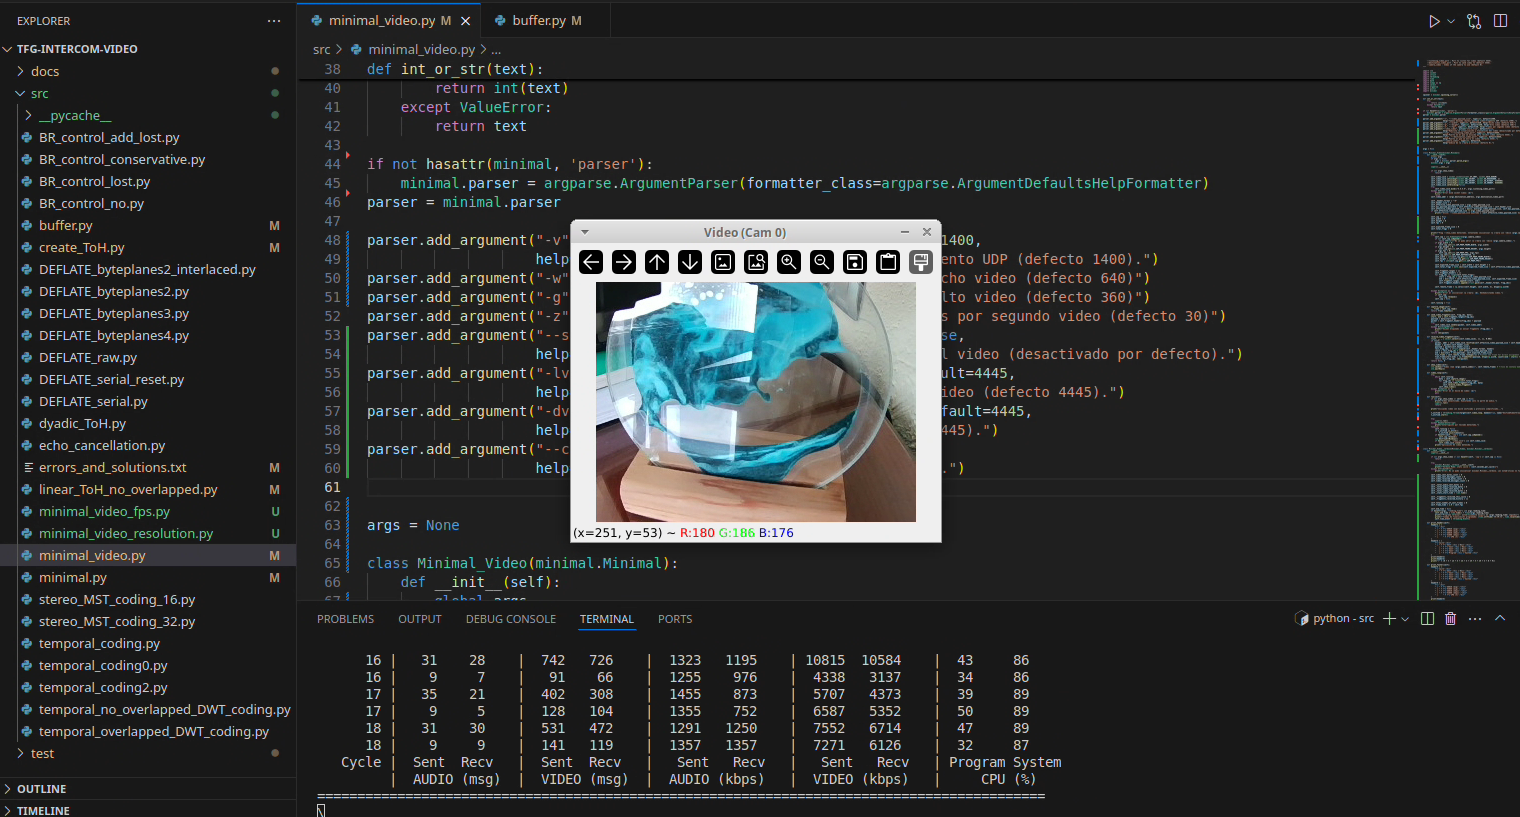
\includegraphics[width=\textwidth,height=0.6\textheight,keepaspectratio]{images/pruebas/ejecuion_normal1.png}
  \end{subfigure}
  \vspace{\baselineskip}
  \begin{subfigure}{\textwidth}
    \centering
    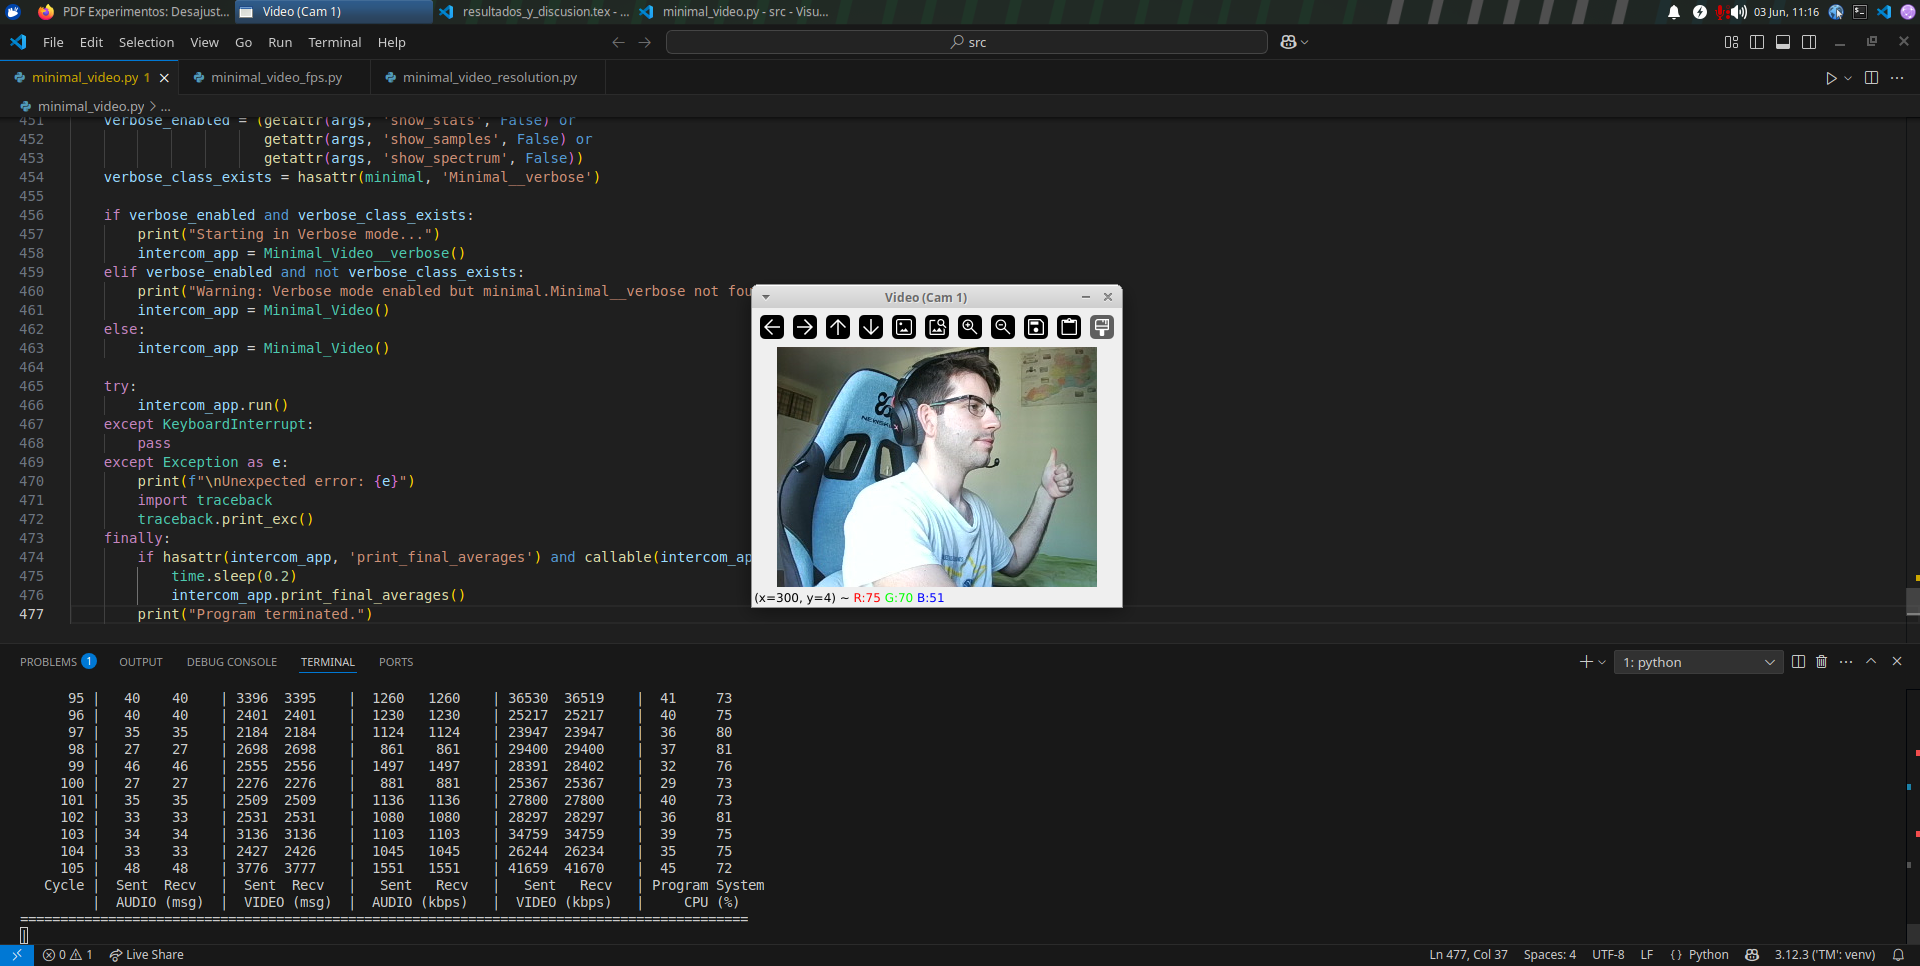
\includegraphics[width=\textwidth,height=0.6\textheight,keepaspectratio]{images/pruebas/ejecuion_normal2.png}
  \end{subfigure}
  \caption{Ejemplo de ejecución común del módulo \textit{Minimal\_Video}.}
  \label{fig:ejecucion_doble}
\end{figure}
\vspace{\baselineskip}

\newpage

Tenemos en primer lugar la inicialización de la biblioteca \texttt{pygame}~\cite{pygame} y el mensaje de bienvenida de la comunidad. A continuación, se muestra el mensaje de inicio del módulo en modo ``verbose'', que es el modo que se ha elegido para esta prueba. En este modo, se muestran estadísticas de la red y del módulo en tiempo real.
\begin{lstlisting}[language=bash,basicstyle=\ttfamily\scriptsize]
pygame 2.6.0 (SDL 2.28.4, Python 3.12.3)
Hello from the pygame community. https://www.pygame.org/contribute.html
(WARNING) minimal: Unable to import argcomplete (optional)
Starting in Verbose mode...
\end{lstlisting}

Seguidamente, se pueden observar un mensaje de que se ha inicializado el vídeo ya que se activó el flag \verb|--show_video| y se ha intentado inicializar la cámara con el índice 1. En este caso, se ha utilizado la cámara del portátil, que es la cámara 0. Si no se encuentra la cámara, se intentará inicializar la cámara con el índice 1. Luego, se ejecuta \textit{Minimal} que es el módulo base que ejecuta el audio el cual proporciona una descripción de distintos parámetros como el chunk\_time, el seconds\_per\_cycle, el chunks\_per\_cycle y el frames\_per\_cycle. Finalmente se indica que se ha iniciado el modo ``verbose''.

\begin{lstlisting}[language=bash,basicstyle=\ttfamily\scriptsize]
Flag --show_video detected. Attempting to initialize camera with index 1...
(INFO) minimal: A minimal InterCom (no compression, no quantization, no transform, 
... only provides a bidirectional (full-duplex) transmission of raw (playable) chunks. 
(INFO) minimal: chunk_time = 0.023219954648526078 seconds
(INFO) minimal: seconds_per_cycle = 1
(INFO) minimal: chunks_per_cycle = 43.06640625
(INFO) minimal: frames_per_cycle = 44100
Verbose Mode: stats cycle = 1s
Starting video with unified loop and simplified protocol (verbose)...
Press Ctrl+C to terminate
\end{lstlisting}

A continuación, se muestra los parámetros inicializados del módulo, así como, los distintos dispositivos que esta usando el sistema.
\begin{lstlisting}[language=bash,basicstyle=\ttfamily\scriptsize]
InterCom parameters:

Namespace(input_device=None, output_device=None, list_devices=False, 
frames_per_second=44100, frames_per_chunk=1024, listening_port=4444, 
destination_address='localhost', destination_port=4444, filename=None, 
reading_time=None, number_of_channels=2, show_stats=True, 
show_samples=False, show_spectrum=False, video_payload_size=1400, 
width=320, height=240, fps=30, show_video=True, listening_video_port=4445, 
destination_video_port=4445, camera_index=1)

Using device:

   0 Intel 82801AA-ICH: - (hw:0,0), ALSA (2 in, 2 out)
   1 Intel 82801AA-ICH: MIC ADC (hw:0,1), ALSA (2 in, 0 out)
   2 Loopback: PCM (hw:1,0), ALSA (32 in, 32 out)
   3 Loopback: PCM (hw:1,1), ALSA (32 in, 32 out)
   4 sysdefault, ALSA (128 in, 128 out)
   5 front, ALSA (0 in, 2 out)
   6 lavrate, ALSA (128 in, 128 out)
   7 samplerate, ALSA (128 in, 128 out)
   8 speexrate, ALSA (128 in, 128 out)
   9 pulse, ALSA (32 in, 32 out)
  10 speex, ALSA (1 in, 1 out)
  11 upmix, ALSA (8 in, 8 out)
  12 vdownmix, ALSA (6 in, 6 out)
  13 dmix, ALSA (0 in, 2 out)
* 14 default, ALSA (32 in, 32 out)
\end{lstlisting}

Continuamos con las estadísticas de la red en cuanto al vídeo y el audio se refiere. En este caso, se muestra el número de mensajes enviados y recibidos, así como, el ancho de banda utilizado en kbps. También se muestra el uso de CPU del módulo y del sistema. En este caso, el uso de CPU del módulo es bastante alto, ya que se está utilizando la cámara y el procesamiento de vídeo en tiempo real. 
\begin{lstlisting}[language=bash,basicstyle=\ttfamily\tiny]
         |  AUDIO (msg)  |  VIDEO (msg)  |  AUDIO (kbps)   |  VIDEO (kbps)   |     CPU (%) 
   Cycle |  Sent  Recv   |  Sent  Recv   |   Sent   Recv   |   Sent   Recv   | Program System
================================================================================================
   Cycle |  Sent  Recv   |  Sent  Recv   |   Sent   Recv   |   Sent   Recv   | Program System
       1 |   10    10    |    3     3    |   303    303    |    31     31    |  33    100       
       2 |   34    34    |  152   152    |  1064   1064    |  1625   1625    |  41     66       
       3 |   40    40    |    0     0    |  1301   1301    |     0      0    |  42     65       
       4 |   44    44    |    0     0    |  1425   1425    |     0      0    |  34     68       
       5 |   42    42    |    0     0    |  1369   1369    |     0      0    |  50     72       
       6 |   43    43    |    0     0    |  1404   1404    |     0      0    |  46     71       
       7 |   40    40    |    0     0    |  1306   1306    |     0      0    |  42     68       
       8 |   39    39    |    0     0    |  1268   1268    |     0      0    |  47     72       
       9 |   38    38    |    0     0    |  1243   1243    |     0      0    |  47     75       
      10 |   40    40    |  597   596    |  1304   1304    |  6648   6637    |  41     73       
      11 |   27    27    | 3035  3036    |   879    879    | 33765  33776    |  48     70       
      12 |   39    39    | 2923  2923    |  1235   1235    | 31610  31610    |  35     75       
      13 |   27    27    | 2898  2897    |   849    849    | 31143  31132    |  54     69       
      14 |   33    33    | 2382  2383    |  1069   1069    | 26347  26358    |  48     74       
      15 |   22    22    | 1815  1815    |   715    715    | 20146  20146    |  32     71       
      16 |   32    32    | 3305  3305    |  1047   1047    | 36934  36934    |  51     74       
      17 |   35    35    | 3460  3460    |  1133   1133    | 38252  38252    |  63     74       
      18 |   27    27    | 3135  3135    |   880    880    | 34909  34909    |  50     70       
   Cycle |  Sent  Recv   |  Sent  Recv   |   Sent   Recv   |   Sent   Recv   | Program System
         |  AUDIO (msg)  |  VIDEO (msg)  |  AUDIO (kbps)   |  VIDEO (kbps)   |     CPU (%) 
===========================================================================================
\end{lstlisting}

Finalmente, se muestra el mensaje de que se ha detectado una interrupción por teclado (Ctrl+C) y se detiene la aplicación de vídeo. A continuación, se muestran las estadísticas globales de ancho de banda, donde se puede observar el ancho de banda utilizado para el audio y el vídeo, así como el tiempo total de ejecución del módulo. Finalmente, se muestra un mensaje de que el módulo ha terminado.
\begin{lstlisting}[language=bash,basicstyle=\ttfamily\scriptsize]
Video application stopped.

=== Global bandwidth statistics ===
Audio sent:       1082.76 kbps
Audio received:   1082.76 kbps
Video sent:       14317.85 kbps
Video received:   14317.85 kbps
Total time:       18.5 s
=====================================
Program terminated.
QObject::killTimer: Timers cannot be stopped from another thread
QObject::~QObject: Timers cannot be stopped from another thread
\end{lstlisting}
\vspace{\baselineskip}

A continuación, un ejemplo de ejecución común de \textit{Minimal\_Video\_FPS} en el que el módulo tratará de cambiar los FPS que vienen por defecto en la cámara (normalmente 30) por el que el usuario solicite por parámetro:
\begin{center}
	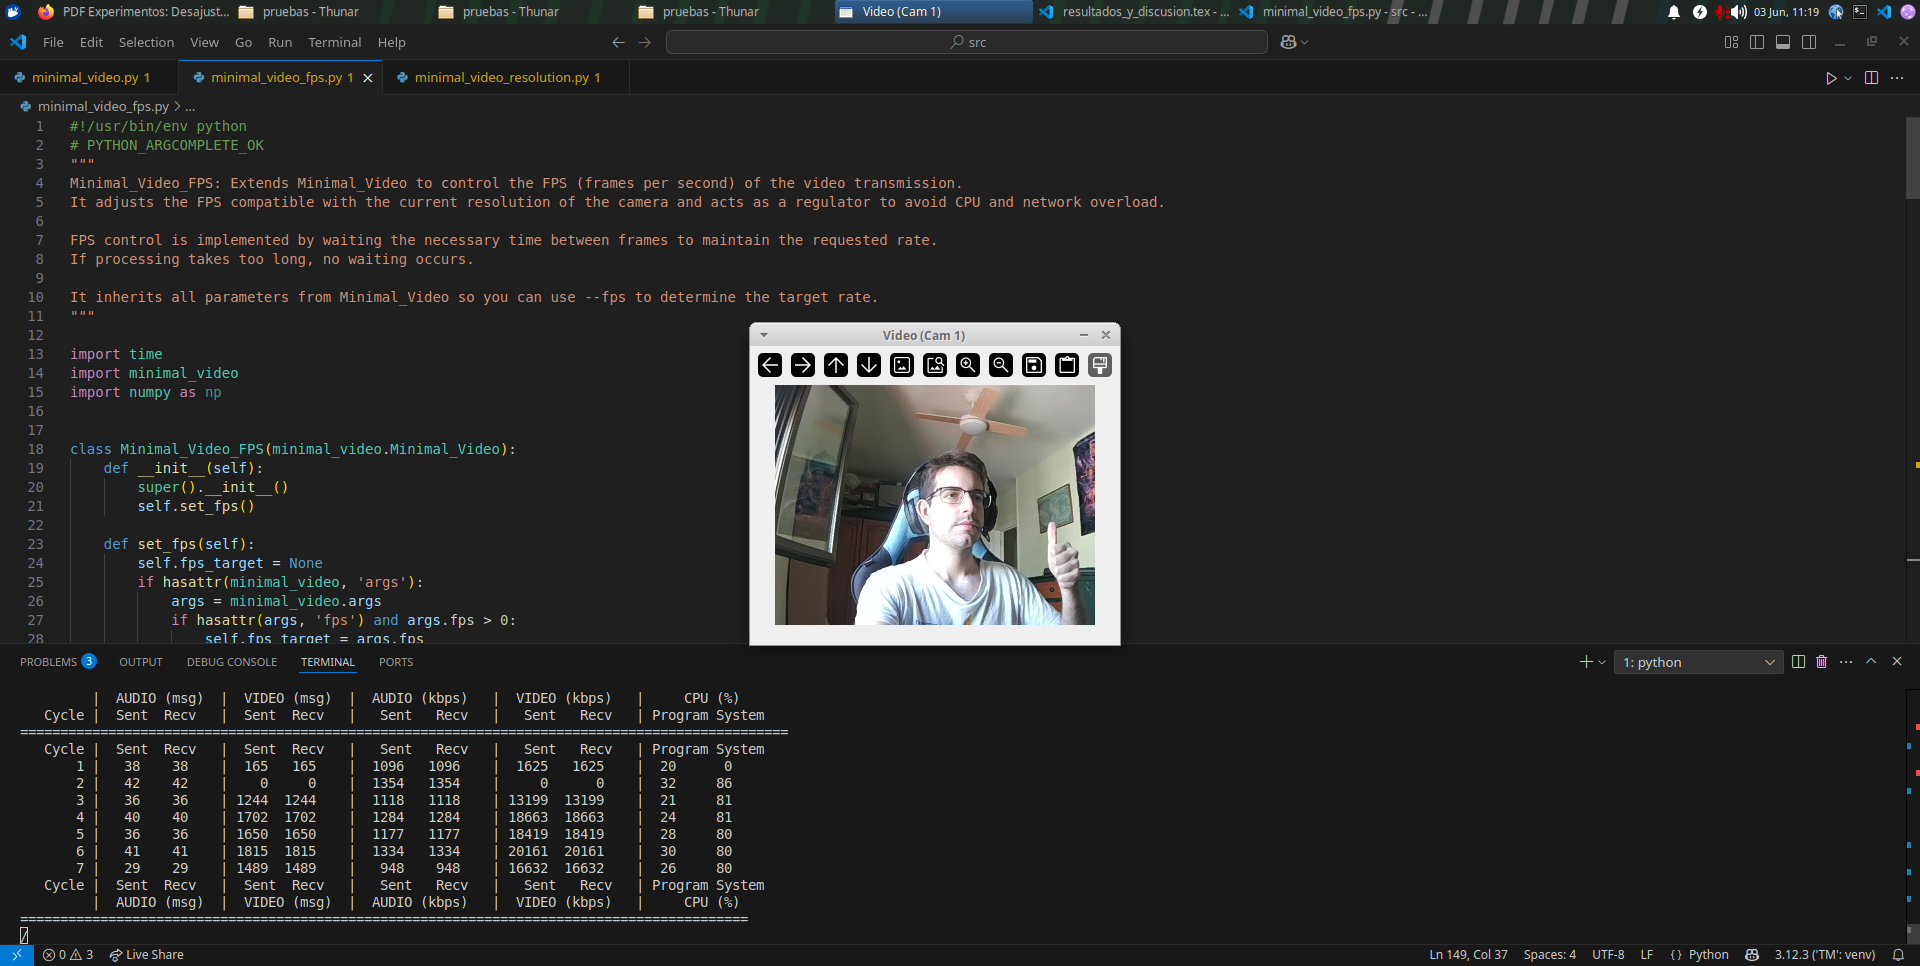
\includegraphics[width = 0.7\textwidth]{images/pruebas/ejecuion_normal_fps.png}
	\captionof{figure}{Ejemplo de ejecución común del módulo \textit{Minimal\_Video\_FPS}.}
	\label{fig:ejecucion_fps}
\end{center}
\vspace{\baselineskip}

\begin{lstlisting}[language=bash,basicstyle=\ttfamily\tiny]
(TM) jj@jj-XubuntuPC:~/TFG-Intercom-Video/src$ python minimal_video_fps.py --show_video 
--show_stats --camera_index 1 -z 12

         |  AUDIO (msg)  |  VIDEO (msg)  |  AUDIO (kbps)   |  VIDEO (kbps)   |     CPU (%) 
   Cycle |  Sent  Recv   |  Sent  Recv   |   Sent   Recv   |   Sent   Recv   | Program System
================================================================================================
       1 |   31    31    |  165   165    |  1012   1012    |  1840   1840    |  13      0       
       2 |   31    31    |  825   825    |  1000   1000    |  9088   9088    |  44     76       
       3 |   35    35    | 1980  1980    |  1145   1145    | 22124  22124    |  45     63       
       4 |   35    35    | 1833  1833    |  1126   1126    | 20144  20144    |  46     61       
       5 |   20    20    | 1137  1137    |   454    454    |  8815   8815    |  41     22       
       6 |   37    37    | 1650  1650    |  1193   1193    | 18175  18175    |  45     70       
       7 |   35    35    | 1980  1980    |  1144   1144    | 22098  22098    |  43     70       
       8 |   33    33    | 1980  1980    |  1079   1079    | 22122  22122    |  49     59       
       9 |   31    31    | 1815  1815    |  1013   1013    | 20253  20253    |  54     71       
      10 |   29    29    | 1980  1980    |   948    948    | 22105  22105    |  48     69       
      11 |   35    35    | 1950  1949    |  1144   1144    | 21775  21764    |  46     70       
      12 |   24    24    | 1845  1846    |   785    785    | 20617  20628    |  46     66       
      13 |   31    31    | 1980  1980    |  1011   1011    | 22063  22063    |  44     67       
      14 |    0     0    |  165   165    |     0      0    |  1843   1843    |   1     19       
   Cycle |  Sent  Recv   |  Sent  Recv   |   Sent   Recv   |   Sent   Recv   | Program System
         |  AUDIO (msg)  |  VIDEO (msg)  |  AUDIO (kbps)   |  VIDEO (kbps)   |     CPU (%) 
===========================================================================================
Video application stopped.

=== Global bandwidth statistics ===
Audio sent:       904.63 kbps
Audio received:   904.63 kbps
Video sent:       16151.39 kbps
Video received:   16151.39 kbps
Total time:       14.7 s
=====================================

=== FPS Statistics ===
Target FPS:       12.0
Average real FPS: 11.8
FPS efficiency:   98.7%
======================
Program terminated.
QObject::killTimer: Timers cannot be stopped from another thread
QObject::~QObject: Timers cannot be stopped from another thread
\end{lstlisting}

\newpage

Finalmente, un ejemplo de ejecución típico de \textit{Minimal\_Video\_Resolution} en el que, por ejemplo en este caso, se le pasa por parámetro que se quiere cambiar de la resolución por defecto del módulo (320x240) a 640x480:
\begin{center}
	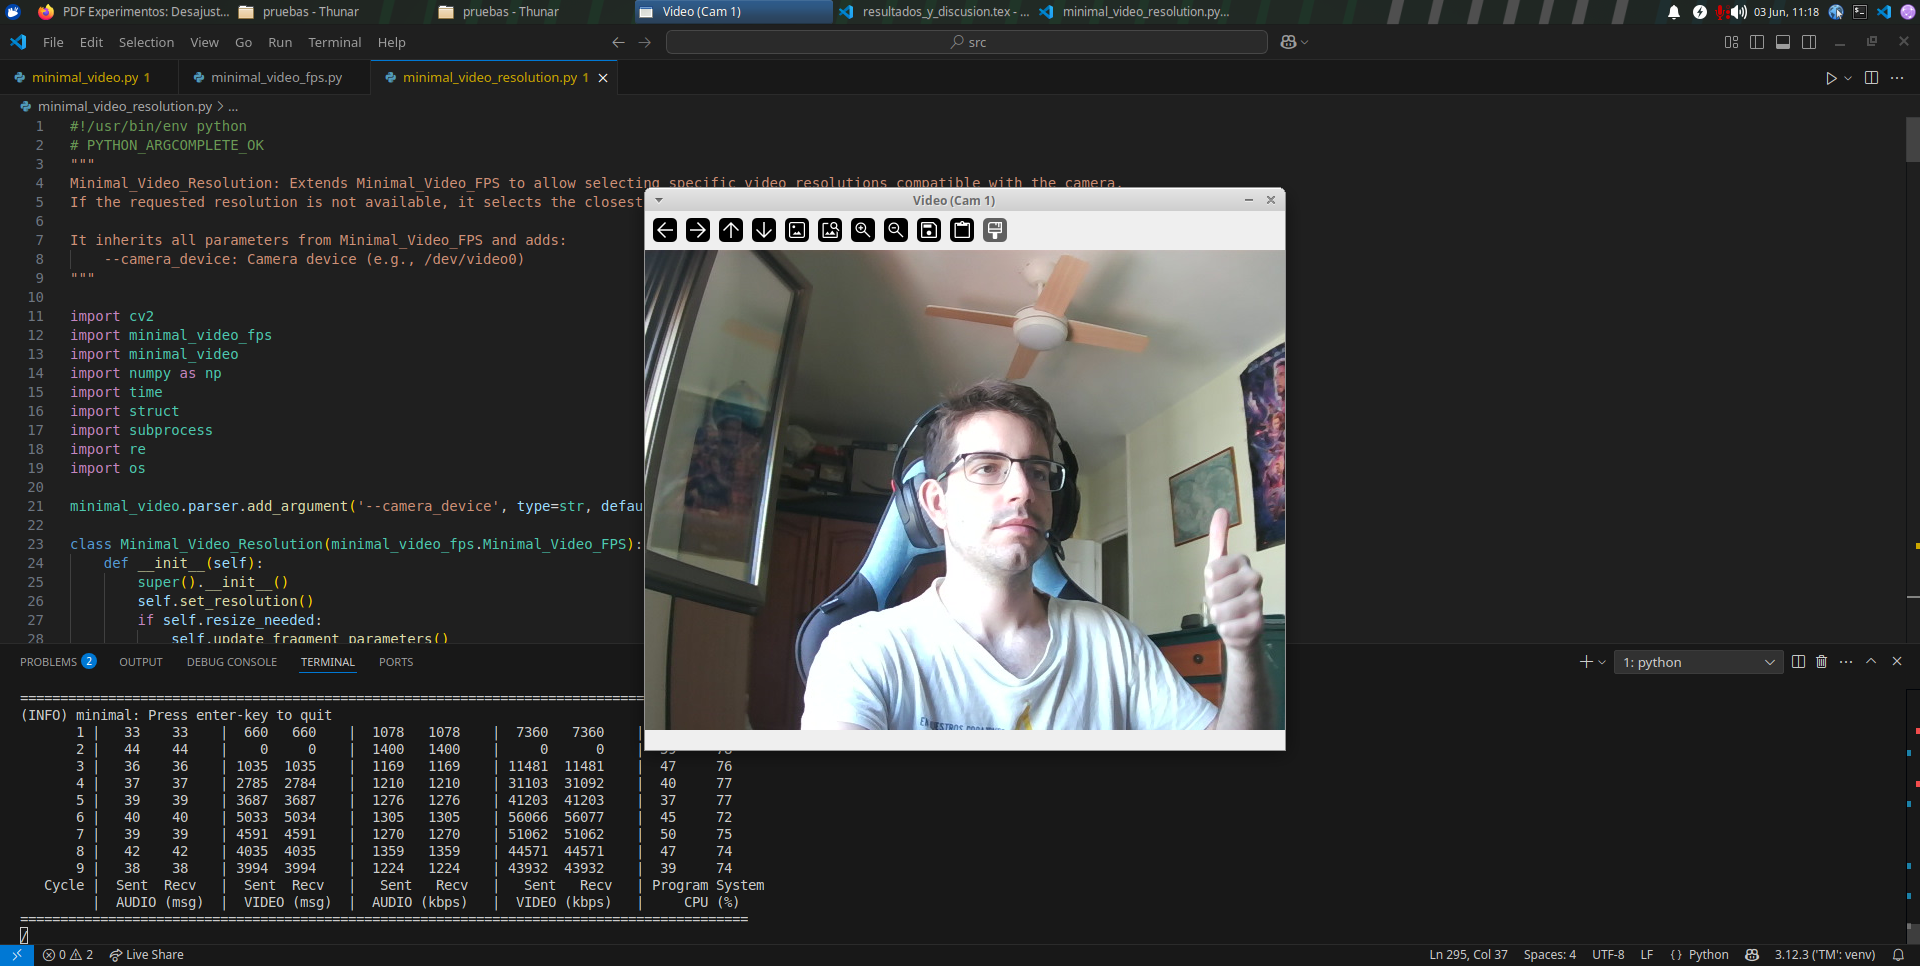
\includegraphics[width = 0.7\textwidth]{images/pruebas/ejecuion_normal_resolution.png}
	\captionof{figure}{Ejemplo de ejecución común del módulo \textit{Minimal\_Video\_Resolution}.}
	\label{fig:ejecucion_resolution}
\end{center}
\vspace{\baselineskip}

\begin{lstlisting}[language=bash,basicstyle=\ttfamily\tiny]
(TM) jj@jj-XubuntuPC:~/TFG-Intercom-Video/src$ python minimal_video_resolution.py --show_video
--show_stats --camera_index 1 -z 12 -w 640 -g 480

         |  AUDIO (msg)  |  VIDEO (msg)  |  AUDIO (kbps)   |  VIDEO (kbps)   |     CPU (%) 
   Cycle |  Sent  Recv   |  Sent  Recv   |   Sent   Recv   |   Sent   Recv   | Program System
================================================================================================
       1 |   25    25    |  660   660    |   817    817    |  7369   7369    |  44      0       
       2 |   33    33    |    0     0    |  1079   1079    |     0      0    |  47     70       
       3 |   33    33    |    0     0    |  1077   1077    |     0      0    |  45     73       
       4 |   24    24    | 2327  2327    |   786    786    | 26022  26022    |  36     69       
       5 |   28    28    | 2972  2972    |   891    891    | 32309  32309    |  35     68       
       6 |   31    31    | 3201  3201    |   999    999    | 35234  35234    |  38     71       
       7 |   17    17    | 3203  3202    |   547    547    | 35250  35239    |  38     70       
       8 |   33    33    | 5376  5376    |  1074   1074    | 59747  59747    |  55     74       
       9 |   34    34    | 5473  5473    |  1109   1109    | 60989  60989    |  55     73       
      10 |   34    34    | 5087  5087    |  1110   1110    | 56718  56718    |  62     72       
      11 |   29    29    | 5689  5689    |   937    937    | 62808  62808    |  60     69       
      12 |   35    35    | 4748  4748    |  1142   1142    | 52914  52914    |  64     73       
      13 |   31    31    | 5399  5399    |  1014   1014    | 60315  60315    |  68     74       
      14 |   26    26    | 4141  4140    |   849    849    | 46197  46186    |  53     66       
      15 |   29    29    | 5402  5402    |   945    945    | 60144  60144    |  56     71       
      16 |    0     0    |  357   358    |     0      0    |  3976   3987    |   0     14       
   Cycle |  Sent  Recv   |  Sent  Recv   |   Sent   Recv   |   Sent   Recv   | Program System
         |  AUDIO (msg)  |  VIDEO (msg)  |  AUDIO (kbps)   |  VIDEO (kbps)   |     CPU (%) 
===========================================================================================
Video application stopped.

=== Global bandwidth statistics ===
Audio sent:       881.25 kbps
Audio received:   881.25 kbps
Video sent:       36779.77 kbps
Video received:   36779.09 kbps
Total time:       16.4 s
=====================================
\end{lstlisting}

\begin{lstlisting}[language=bash,basicstyle=\ttfamily\scriptsize]
=== FPS Statistics ===
Target FPS:       12.0
Average real FPS: 7.4
FPS efficiency:   61.8%
======================

=== Camera compatible resolutions ===
  1. 320x240
  2. 352x288
  3. 640x360
  4. 640x480 * SELECTED
  5. 800x600
  6. 1024x768
  7. 1280x720
  8. 1280x1024
  9. 1366x768
  10. 1600x900
  11. 1920x1080
  12. 2560x1440
  13. 3840x2160

Camera device: /dev/video0
======================================
Program terminated.
QObject::killTimer: Timers cannot be stopped from another thread
QObject::~QObject: Timers cannot be stopped from another thread
\end{lstlisting}
\vspace{\baselineskip}

\newpage

\subsubsection{Experimentos con limitación de la tasa de transferencia de datos}

En esta sección se presentan los resultados obtenidos al ejecutar los módulos bajo diferentes condiciones de ancho de banda. 
\vspace{\baselineskip}

\begin{itemize}
    \item \textbf{Pruebas de limitación de la tasa de transferencia}:
\end{itemize}

\textbf{Pruebas de limitación de la tasa de transferencia a 1 Mbps}
\vspace{\baselineskip}

Empezaremos por probar el módulo con un ancho de banda muy bajo, 1 Mbps. El comando usado para \textit{Minimal\_Video} ha sido el siguiente:

\begin{lstlisting}[language=bash]
python minimal_video.py -a 192.168.0.58 --show_video --show_stats
\end{lstlisting}
Donde \verb|-a| es la dirección IP del dispositivo con el que se va a comunicar el módulo, \verb|--show_video| es la opción para mostrar el vídeo en tiempo real y \verb|--show_stats| es la opción para mostrar las estadísticas de la red.
\vspace{\baselineskip}

\begin{lstlisting}[language=bash,basicstyle=\ttfamily\tiny]
         |  AUDIO (msg)  |  VIDEO (msg)  |  AUDIO (kbps)   |  VIDEO (kbps)   |     CPU (%) 
   Cycle |  Sent  Recv   |  Sent  Recv   |   Sent   Recv   |   Sent   Recv   | Program System
================================================================================================
       1 |   27     6    |  165   146    |   881    195    |  1838   1628    |  36      0       
       2 |   33    28    |    0     0    |  1073    910    |     0      0    |  41     75       
       3 |   37     1    |    0     0    |  1206     32    |     0      0    |  51     74       
   Cycle |  Sent  Recv   |  Sent  Recv   |   Sent   Recv   |   Sent   Recv   | Program System
         |  AUDIO (msg)  |  VIDEO (msg)  |  AUDIO (kbps)   |  VIDEO (kbps)   |     CPU (%) 
===========================================================================================
\end{lstlisting}


\begin{lstlisting}[language=bash,basicstyle=\ttfamily\tiny]
Socket blocked while sending fragment 20.
Socket blocked while sending fragment 21.
Socket blocked while sending fragment 22.
Socket blocked while sending fragment 23.
Socket blocked while sending fragment 24.
Socket blocked while sending fragment 25.
Socket blocked while sending fragment 26.
Socket blocked while sending fragment 27.
Socket blocked while sending fragment 28.
Socket blocked while sending fragment 29.
Socket blocked while sending fragment 30.
Socket blocked while sending fragment 31.
Socket blocked while sending fragment 32.
Socket blocked while sending fragment 33.
Socket blocked while sending fragment 34.
Socket blocked while sending fragment 35.
Socket blocked while sending fragment 36.
Socket blocked while sending fragment 37.
Socket blocked while sending fragment 38.
Socket blocked while sending fragment 39.
Socket blocked while sending fragment 40.
Socket blocked while sending fragment 41.
Socket blocked while sending fragment 42.
Socket blocked while sending fragment 43.
Socket blocked while sending fragment 44.
Socket blocked while sending fragment 45.

       4 |   32     3    |  275   187    |  1044     97    |  3065   2081    |  43     73       
   Cycle |  Sent  Recv   |  Sent  Recv   |   Sent   Recv   |   Sent   Recv   | Program System
         |  AUDIO (msg)  |  VIDEO (msg)  |  AUDIO (kbps)   |  VIDEO (kbps)   |     CPU (%) 
===========================================================================================
Socket blocked while sending fragment 110.
Socket blocked while sending fragment 111.
Socket blocked while sending fragment 112.
Socket blocked while sending fragment 113.
Socket blocked while sending fragment 114.
Socket blocked while sending fragment 115.
Socket blocked while sending fragment 116.
Socket blocked while sending fragment 117.
Socket blocked while sending fragment 118.
Socket blocked while sending fragment 119.
Socket blocked while sending fragment 120.
Socket blocked while sending fragment 121.
Socket blocked while sending fragment 122.
Socket blocked while sending fragment 123.
Socket blocked while sending fragment 124.
Socket blocked while sending fragment 125.
Socket blocked while sending fragment 126.
Socket blocked while sending fragment 127.
Socket blocked while sending fragment 128.
Socket blocked while sending fragment 129.
Socket blocked while sending fragment 130.
Socket blocked while sending fragment 131.
Socket blocked while sending fragment 132.
Socket blocked while sending fragment 133.
Socket blocked while sending fragment 134.
Socket blocked while sending fragment 135.
Socket blocked while sending fragment 136.
Socket blocked while sending fragment 137.
Socket blocked while sending fragment 138.
Socket blocked while sending fragment 139.
Socket blocked while sending fragment 140.
Socket blocked while sending fragment 141.
Socket blocked while sending fragment 142.
Socket blocked while sending fragment 143.
Socket blocked while sending fragment 144.
Socket blocked while sending fragment 145.
Socket blocked while sending fragment 146.
Socket blocked while sending fragment 147.
Socket blocked while sending fragment 148.
Socket blocked while sending fragment 149.
Socket blocked while sending fragment 150.
Socket blocked while sending fragment 151.
Socket blocked while sending fragment 152.
Socket blocked while sending fragment 153.
Socket blocked while sending fragment 154.
Socket blocked while sending fragment 155.
Socket blocked while sending fragment 156.
Socket blocked while sending fragment 157.
Socket blocked while sending fragment 158.
Socket blocked while sending fragment 159.
Socket blocked while sending fragment 160.
Socket blocked while sending fragment 161.
Socket blocked while sending fragment 162.
Socket blocked while sending fragment 163.
Socket blocked while sending fragment 164.

       5 |   29    21    |  274    17    |   946    685    |  3051    189    |  27     76       
   Cycle |  Sent  Recv   |  Sent  Recv   |   Sent   Recv   |   Sent   Recv   | Program System
         |  AUDIO (msg)  |  VIDEO (msg)  |  AUDIO (kbps)   |  VIDEO (kbps)   |     CPU (%) 
===========================================================================================
Socket blocked while sending fragment 42.
Socket blocked while sending fragment 43.
Socket blocked while sending fragment 44.
Socket blocked while sending fragment 45.
Socket blocked while sending fragment 46.
Socket blocked while sending fragment 47.
Socket blocked while sending fragment 48.
Socket blocked while sending fragment 49.
Socket blocked while sending fragment 50.
Socket blocked while sending fragment 51.
Socket blocked while sending fragment 52.
Socket blocked while sending fragment 53.
Socket blocked while sending fragment 54.
Socket blocked while sending fragment 55.
Socket blocked while sending fragment 56.
Socket blocked while sending fragment 57.
Socket blocked while sending fragment 58.
Socket blocked while sending fragment 59.
Socket blocked while sending fragment 60.
Socket blocked while sending fragment 61.
Socket blocked while sending fragment 62.
Socket blocked while sending fragment 63.
Socket blocked while sending fragment 64.
Socket blocked while sending fragment 65.
Socket blocked while sending fragment 66.
Socket blocked while sending fragment 67.
Socket blocked while sending fragment 68.
Socket blocked while sending fragment 69.
Socket blocked while sending fragment 70.
Socket blocked while sending fragment 71.
Socket blocked while sending fragment 72.
Socket blocked while sending fragment 73.
Socket blocked while sending fragment 74.
Socket blocked while sending fragment 75.
Socket blocked while sending fragment 76.
Socket blocked while sending fragment 77.
Socket blocked while sending fragment 78.
Socket blocked while sending fragment 79.
Socket blocked while sending fragment 80.
Socket blocked while sending fragment 81.
Socket blocked while sending fragment 82.
Socket blocked while sending fragment 83.
Socket blocked while sending fragment 84.
Socket blocked while sending fragment 85.
Socket blocked while sending fragment 86.
Socket blocked while sending fragment 87.

       6 |   24     7    |  276    76    |   785    228    |  3081    847    |  24     66       
   Cycle |  Sent  Recv   |  Sent  Recv   |   Sent   Recv   |   Sent   Recv   | Program System
         |  AUDIO (msg)  |  VIDEO (msg)  |  AUDIO (kbps)   |  VIDEO (kbps)   |     CPU (%) 
===========================================================================================
Video application stopped.

=== Global bandwidth statistics ===
Audio sent:       954.02 kbps
Audio received:   345.96 kbps
Video sent:       1771.67 kbps
Video received:   762.21 kbps
Total time:       6.3 s
=====================================
Program terminated.
QObject::killTimer: Timers cannot be stopped from another thread
QObject::~QObject: Timers cannot be stopped from another thread
\end{lstlisting}
\vspace{\baselineskip}

La imagen de la Figura \ref{fig:minimal_video_1mbps} es una captura del vídeo recibido en esta prueba.
\begin{center}
  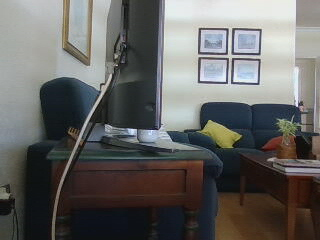
\includegraphics[width = 0.7\textwidth]{images/VideoRecibido1.1.png}
  \captionof{figure}{Vídeo recibido en \textit{Minimal\_Video} para ancho de banda de 1 Mbps.}
  \label{fig:minimal_video_1mbps}
\end{center}

\newpage

\vspace{\baselineskip}

Ahora, ejecutaremos el módulo \textit{Minimal\_Video\_FPS} con el mismo ancho de banda, 1 Mbps. El comando usado ha sido el siguiente:

\begin{lstlisting}[language=bash, basicstyle=\ttfamily\scriptsize]
    python minimal_video_fps.py -a 192.168.0.58 --show_video --show_stats -z 12
\end{lstlisting}

Donde \verb|-a| es la dirección IP destino, \verb|--show_video| es para que se active la transmisión de vídeo, \verb|--show_stats| es para que se muestre la información de estadísticas y \verb|-z| es el numero de fotogramas por segundo (FPS) que se desea enviar. En este caso, se ha configurado para mostrar el vídeo a 12 FPS.

A continuación, se probará el módulo con un ancho de banda muy bajo, de 1 Mbps. El resultado obtenido ha sido el siguiente:
\vspace{\baselineskip}

\begin{lstlisting}[language=bash,basicstyle=\ttfamily\tiny]
         |  AUDIO (msg)  |  VIDEO (msg)  |  AUDIO (kbps)   |  VIDEO (kbps)   |     CPU (%) 
   Cycle |  Sent  Recv   |  Sent  Recv   |   Sent   Recv   |   Sent   Recv   | Program System
================================================================================================
       1 |   25    25    |  165    92    |   810    810    |  1826   1019    |  21    100       
       2 |   36     7    |    0     0    |  1141    221    |     0      0    |  43     76       
       3 |   37    25    |    0     0    |  1208    816    |     0      0    |  44     75       
       4 |   20     0    |  330   157    |   653      0    |  3681   1751    |  21     69       
   Cycle |  Sent  Recv   |  Sent  Recv   |   Sent   Recv   |   Sent   Recv   | Program System
         |  AUDIO (msg)  |  VIDEO (msg)  |  AUDIO (kbps)   |  VIDEO (kbps)   |     CPU (%) 
===========================================================================================
\end{lstlisting}

\begin{lstlisting}[language=bash,basicstyle=\ttfamily\tiny]
Socket blocked while sending fragment 43.
Socket blocked while sending fragment 44.
Socket blocked while sending fragment 45.
Socket blocked while sending fragment 49.
Socket blocked while sending fragment 50.
Socket blocked while sending fragment 52.
Socket blocked while sending fragment 53.
Socket blocked while sending fragment 54.
Socket blocked while sending fragment 55.
Socket blocked while sending fragment 56.
Socket blocked while sending fragment 58.
Socket blocked while sending fragment 61.
Socket blocked while sending fragment 62.
Socket blocked while sending fragment 63.
Socket blocked while sending fragment 64.
Socket blocked while sending fragment 65.
Socket blocked while sending fragment 68.
Socket blocked while sending fragment 69.
Socket blocked while sending fragment 71.
Socket blocked while sending fragment 74.
Socket blocked while sending fragment 75.
Socket blocked while sending fragment 79.
Socket blocked while sending fragment 80.
Socket blocked while sending fragment 81.
Socket blocked while sending fragment 82.
Socket blocked while sending fragment 83.
Socket blocked while sending fragment 84.
Socket blocked while sending fragment 85.
Socket blocked while sending fragment 86.
Socket blocked while sending fragment 89.
Socket blocked while sending fragment 90.
Socket blocked while sending fragment 91.
Socket blocked while sending fragment 93.
Socket blocked while sending fragment 94.
Socket blocked while sending fragment 95.
Socket blocked while sending fragment 97.
Socket blocked while sending fragment 98.
Socket blocked while sending fragment 99.

       5 |   31     6    |  323    87    |  1015    196    |  3613    971    |  33     68       
   Cycle |  Sent  Recv   |  Sent  Recv   |   Sent   Recv   |   Sent   Recv   | Program System
         |  AUDIO (msg)  |  VIDEO (msg)  |  AUDIO (kbps)   |  VIDEO (kbps)   |     CPU (%) 
===========================================================================================
Socket blocked while sending fragment 61.
Socket blocked while sending fragment 62.
Socket blocked while sending fragment 63.
Socket blocked while sending fragment 64.
Socket blocked while sending fragment 65.
Socket blocked while sending fragment 66.
Socket blocked while sending fragment 69.
Socket blocked while sending fragment 71.
Socket blocked while sending fragment 73.
Socket blocked while sending fragment 74.
Socket blocked while sending fragment 75.
Socket blocked while sending fragment 76.
Socket blocked while sending fragment 77.
Socket blocked while sending fragment 78.
Socket blocked while sending fragment 80.
Socket blocked while sending fragment 81.
Socket blocked while sending fragment 83.
Socket blocked while sending fragment 84.
Socket blocked while sending fragment 86.
Socket blocked while sending fragment 87.
Socket blocked while sending fragment 88.
Socket blocked while sending fragment 89.
Socket blocked while sending fragment 90.
Socket blocked while sending fragment 91.
Socket blocked while sending fragment 93.
Socket blocked while sending fragment 94.
Socket blocked while sending fragment 95.
Socket blocked while sending fragment 96.
Socket blocked while sending fragment 99.
Socket blocked while sending fragment 100.
Socket blocked while sending fragment 101.
Socket blocked while sending fragment 102.
Socket blocked while sending fragment 103.
Socket blocked while sending fragment 104.
Socket blocked while sending fragment 106.
Socket blocked while sending fragment 108.
Socket blocked while sending fragment 109.
Socket blocked while sending fragment 111.
Socket blocked while sending fragment 113.
Socket blocked while sending fragment 114.
Socket blocked while sending fragment 115.
Socket blocked while sending fragment 116.
Socket blocked while sending fragment 118.
Socket blocked while sending fragment 119.
Socket blocked while sending fragment 120.
Socket blocked while sending fragment 121.
Socket blocked while sending fragment 122.
Socket blocked while sending fragment 124.
Socket blocked while sending fragment 125.
Socket blocked while sending fragment 126.
Socket blocked while sending fragment 127.
Socket blocked while sending fragment 129.
Socket blocked while sending fragment 130.
Socket blocked while sending fragment 131.
Socket blocked while sending fragment 133.
Socket blocked while sending fragment 136.
Socket blocked while sending fragment 137.
Socket blocked while sending fragment 138.
Socket blocked while sending fragment 139.
Socket blocked while sending fragment 140.
Socket blocked while sending fragment 142.
Socket blocked while sending fragment 143.
Socket blocked while sending fragment 145.
Socket blocked while sending fragment 146.
Socket blocked while sending fragment 147.
Socket blocked while sending fragment 149.
Socket blocked while sending fragment 151.
Socket blocked while sending fragment 152.
Socket blocked while sending fragment 153.
Socket blocked while sending fragment 154.
Socket blocked while sending fragment 155.
Socket blocked while sending fragment 156.
Socket blocked while sending fragment 160.
Socket blocked while sending fragment 161.
Socket blocked while sending fragment 162.
Socket blocked while sending fragment 164.

       6 |   26    16    |  283    15    |   850    523    |  3160    167    |  22     69       
   Cycle |  Sent  Recv   |  Sent  Recv   |   Sent   Recv   |   Sent   Recv   | Program System
         |  AUDIO (msg)  |  VIDEO (msg)  |  AUDIO (kbps)   |  VIDEO (kbps)   |     CPU (%) 
===========================================================================================
Socket blocked while sending fragment 44.
Socket blocked while sending fragment 46.
Socket blocked while sending fragment 47.
Socket blocked while sending fragment 49.
Socket blocked while sending fragment 50.
Socket blocked while sending fragment 51.
Keyboard interrupt detected.

Video application stopped.

=== Global bandwidth statistics ===
Audio sent:       867.25 kbps
Audio received:   391.50 kbps
Video sent:       1862.96 kbps
Video received:   593.89 kbps
Total time:       6.6 s
=====================================

=== FPS Statistics ===
Target FPS:       12.0
Average real FPS: 1.0
FPS efficiency:   8.3%
======================
\end{lstlisting}

\newpage

La imagen de la Figura \ref{fig:minimal_video_fps_1mbps} es una captura del vídeo recibido en esta prueba.
\begin{center}
  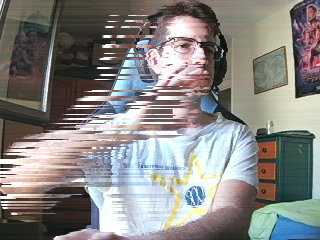
\includegraphics[width = 0.7\textwidth]{images/VideoRecibido1.2.png}
  \captionof{figure}{Vídeo recibido en \textit{Minimal\_Video\_FPS} para ancho de banda de 1 Mbps.}
  \label{fig:minimal_video_fps_1mbps}
\end{center}

\newpage

Finalmente, se ejecutará el módulo \textit{Minimal\_Video\_Resolution} con el mismo ancho de banda, 1 Mbps. El comando usado ha sido el siguiente:
\begin{lstlisting}[language=bash,basicstyle=\ttfamily\scriptsize]
python minimal_video_resolution.py -a 192.168.0.58 --show_video --show_stats -z 12 \\
-w 350 -g 250
\end{lstlisting}
Donde \verb|-a| indica la dirección IP destino, \verb|--show_video| indica que se active la transmisión de vídeo, \verb|--show_stats| indica que se muestren las estadísticas de la transmisión, \verb|-z| indica el número de fotogramas por segundo (FPS), \verb|-w| indica el ancho del vídeo y \verb|-g| indica la altura del vídeo.
\vspace{\baselineskip}

\begin{lstlisting}[language=bash,basicstyle=\ttfamily\tiny]
         |  AUDIO (msg)  |  VIDEO (msg)  |  AUDIO (kbps)   |  VIDEO (kbps)   |     CPU (%) 
   Cycle |  Sent  Recv   |  Sent  Recv   |   Sent   Recv   |   Sent   Recv   | Program System
================================================================================================
       1 |   24    24    |  188   103    |   785    785    |  2101   1152    |  20      0       
       2 |   31     7    |  131    79    |  1006    227    |  1453    876    |  23     70       
   Cycle |  Sent  Recv   |  Sent  Recv   |   Sent   Recv   |   Sent   Recv   | Program System
         |  AUDIO (msg)  |  VIDEO (msg)  |  AUDIO (kbps)   |  VIDEO (kbps)   |     CPU (%) 
===========================================================================================
\end{lstlisting}

\begin{lstlisting}[language=bash,basicstyle=\ttfamily\tiny]
Socket blocked while sending fragment 2.
Socket blocked while sending fragment 3.
Socket blocked while sending fragment 4.
Socket blocked while sending fragment 5.
Socket blocked while sending fragment 6.
Socket blocked while sending fragment 7.
Socket blocked while sending fragment 8.
Socket blocked while sending fragment 9.
Socket blocked while sending fragment 10.
Socket blocked while sending fragment 11.
Socket blocked while sending fragment 12.
Socket blocked while sending fragment 13.
Socket blocked while sending fragment 14.
Socket blocked while sending fragment 15.
Socket blocked while sending fragment 16.
Socket blocked while sending fragment 17.
Socket blocked while sending fragment 18.
Socket blocked while sending fragment 19.
Socket blocked while sending fragment 20.
Socket blocked while sending fragment 21.
Socket blocked while sending fragment 22.
Socket blocked while sending fragment 23.
Socket blocked while sending fragment 24.
Socket blocked while sending fragment 25.
Socket blocked while sending fragment 26.
Socket blocked while sending fragment 27.
Socket blocked while sending fragment 28.
Socket blocked while sending fragment 29.
Socket blocked while sending fragment 30.
Socket blocked while sending fragment 31.
Socket blocked while sending fragment 32.
Socket blocked while sending fragment 33.
Socket blocked while sending fragment 34.
Socket blocked while sending fragment 35.
Socket blocked while sending fragment 36.
Socket blocked while sending fragment 37.
Socket blocked while sending fragment 38.
Socket blocked while sending fragment 39.
Socket blocked while sending fragment 40.
Socket blocked while sending fragment 41.
Socket blocked while sending fragment 42.
Socket blocked while sending fragment 43.
Socket blocked while sending fragment 44.
Socket blocked while sending fragment 45.
Socket blocked while sending fragment 46.
Socket blocked while sending fragment 47.
Socket blocked while sending fragment 48.
Socket blocked while sending fragment 49.
Socket blocked while sending fragment 50.
Socket blocked while sending fragment 51.
Socket blocked while sending fragment 52.
Socket blocked while sending fragment 53.
Socket blocked while sending fragment 54.
Socket blocked while sending fragment 55.
Socket blocked while sending fragment 56.
       3 |   27    20    |  273     6    |   871    645    |  3007     63    |  41     72       
   Cycle |  Sent  Recv   |  Sent  Recv   |   Sent   Recv   |   Sent   Recv   | Program System
         |  AUDIO (msg)  |  VIDEO (msg)  |  AUDIO (kbps)   |  VIDEO (kbps)   |     CPU (%) 
===========================================================================================
Socket blocked while sending fragment 28.
Socket blocked while sending fragment 29.
Socket blocked while sending fragment 30.
Socket blocked while sending fragment 31.
Socket blocked while sending fragment 33.
Socket blocked while sending fragment 34.
Socket blocked while sending fragment 36.
Socket blocked while sending fragment 37.
Socket blocked while sending fragment 38.
Socket blocked while sending fragment 39.
Socket blocked while sending fragment 41.
Socket blocked while sending fragment 42.
Socket blocked while sending fragment 43.
Socket blocked while sending fragment 44.
Socket blocked while sending fragment 45.
Socket blocked while sending fragment 47.
Socket blocked while sending fragment 48.
Socket blocked while sending fragment 49.
Socket blocked while sending fragment 50.
Socket blocked while sending fragment 51.

       4 |   28     9    |  336    86    |   891    286    |  3655    936    |  33     66       
   Cycle |  Sent  Recv   |  Sent  Recv   |   Sent   Recv   |   Sent   Recv   | Program System
         |  AUDIO (msg)  |  VIDEO (msg)  |  AUDIO (kbps)   |  VIDEO (kbps)   |     CPU (%) 
===========================================================================================
Socket blocked while sending fragment 177.
Socket blocked while sending fragment 178.
Socket blocked while sending fragment 179.
Socket blocked while sending fragment 181.
Socket blocked while sending fragment 182.
Socket blocked while sending fragment 183.
Socket blocked while sending fragment 184.
Socket blocked while sending fragment 185.
Socket blocked while sending fragment 187.
       5 |   13     0    |  200    50    |   425      0    |  2231    559    |  16     59       
   Cycle |  Sent  Recv   |  Sent  Recv   |   Sent   Recv   |   Sent   Recv   | Program System
         |  AUDIO (msg)  |  VIDEO (msg)  |  AUDIO (kbps)   |  VIDEO (kbps)   |     CPU (%) 
===========================================================================================
Keyboard interrupt detected.

Video application stopped.

=== Global bandwidth statistics ===
Audio sent:       738.20 kbps
Audio received:   360.10 kbps
Video sent:       2311.06 kbps
Video received:   664.16 kbps
Total time:       5.5 s
=====================================

=== FPS Statistics ===
Target FPS:       12.0
Average real FPS: 1.1
FPS efficiency:   8.9%
======================

=== Resolution Statistics ===
Target resolution: 350x250
Actual resolution: 352x288
Average rescaling time: 3.05 ms
Performance impact:     3.7%
=============================

=== Camera compatible resolutions ===
  1. 320x240
  2. 352x288 * SELECTED
  3. 640x360
  4. 640x480
  5. 800x600
  6. 1024x768
  7. 1280x720
  8. 1280x1024
  9. 1366x768
  10. 1600x900
  11. 1920x1080
  12. 2560x1440
  13. 3840x2160

Camera device: /dev/video0
======================================
Program terminated.
QObject::killTimer: Timers cannot be stopped from another thread
QObject::~QObject: Timers cannot be stopped from another thread
\end{lstlisting}
\vspace{\baselineskip}

\newpage

La imagen de la Figura \ref{fig:minimal_video_resolution_1mbps} es una captura del vídeo recibido en esta prueba.
\begin{center}
  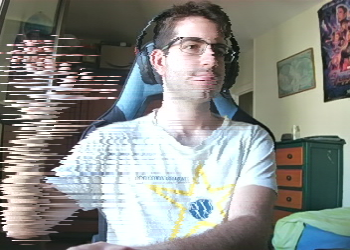
\includegraphics[width = 0.7\textwidth]{images/VideoRecibido1.3.png}
  \captionof{figure}{Vídeo recibido en \textit{Minimal\_Video\_Resolution} para ancho de banda de 1 Mbps.}
  \label{fig:minimal_video_resolution_1mbps}
\end{center}

\newpage

Ahora, se procederá a extraer las conclusiones correspondientes a las pruebas realizadas con un ancho de banda muy bajo, 1 Mbps.

\vspace{\baselineskip}

\textbf{Análisis de \textit{Minimal\_Video} con 1 Mbps de tasa de transferencia:}
\vspace{\baselineskip}

Al observar la salida de \textit{Minimal\_Video} bajo esta limitación de red, se aprecian varios puntos clave. En los primeros ciclos de ejecución del módulo, se intenta enviar el vídeo (por ejemplo, en el ciclo 1, se envían 1838 kbps de vídeo y se reciben 1628 kbps, mostrando un intento inicial antes de la saturación). Luego, las estadísticas globales muestran que se intentó enviar 1771.67 kbps de vídeo, pero solo se recibieron 762.21 kbps. Para el audio, las cifras son: 954.02 kbps enviados y 345.96 kbps recibidos.
\vspace{\baselineskip}

La aparición constante de mensajes como ``Socket bloqueado al enviar fragmento X'' indica que la red no puede manejar el volumen de datos que el módulo intenta transmitir. El módulo está generando datos (especialmente de vídeo) a una tasa que supera significativamente el límite de 1 Mbps. Esto da como resultado que una gran cantidad de paquetes se pierdan o se retrasen, haciendo que la experiencia de usuario sea muy deficiente, con el vídeo viéndose durante bastante tiempo entrecortado y congelado, así como un audio de mala calidad. A pesar de todo, se puede comprobar que una parte del vídeo y el audio consigue llegar al destinatario, aunque la calidad es muy pobre.

\vspace{\baselineskip}

\textbf{Análisis de \textit{Minimal\_Video\_FPS} con 1 Mbps de tasa de transferencia:}
\vspace{\baselineskip}

Este módulo, al estar bajo la misma limitación de 1 Mbps, muestra resultados similares.
\vspace{\baselineskip}

Las estadísticas globales muestran un intento de envío de 1862.96 kbps de vídeo (con 593.89 kbps recibidos) y 867.25 kbps de audio (con 391.50 kbps recibidos). Sin embargo, lo realmente importante en este módulo es ver si se consigue llegar a los 12 FPS objetivo, pero el promedio real fue de solo 1.0 FPS, con una eficiencia del 8.3\%. Esto demuestra que, aunque el módulo intenta gestionar la tasa de fotogramas, la limitación del ancho de banda impide alcanzar el objetivo. El módulo no puede enviar los 12 fotogramas deseados por segundo porque no hay suficiente ancho de banda. Los mensajes de ``Socket bloqueado'' siguen apareciendo, confirmando la congestión. La cantidad total de vídeo enviado es alta, y aunque el control de FPS intenta reducir la carga por fotograma para cumplir el objetivo, la tasa de envío global sigue siendo excesiva para 1 Mbps.

\vspace{\baselineskip}

\textbf{Análisis de \textit{Minimal\_Video\_Resolution} con 1 Mbps de tasa de transferencia:}
\vspace{\baselineskip}

Este módulo trata de reescalar la resolución del vídeo (en este caso, a 350x250, aunque la cámara selecciona la más cercana compatible que es 352x288) además de mantener el objetivo de conseguir 12 FPS. Los resultados con la limitación de 1 Mbps de ancho de banda siguen siendo muy deficientes.
\vspace{\baselineskip}

Las estadísticas globales indican que se intentó enviar 2311.06 kbps de vídeo y 738.20 kbps de audio, de los cuales se recibieron 664.16 kbps de vídeo y 360.10 kbps de audio. Los FPS reales promedio fueron de 1.1, con una eficiencia del 8.9\%, muy parecido al módulo anterior. Aunque se recibió algo de vídeo y audio, la cantidad de datos que se intentan enviar sigue superando con creces la capacidad de la red. Los mensajes de ``Socket bloqueado'' son persistentes, indicando que el módulo está intentando enviar datos que la red no puede transmitir. La combinación de intentar conseguir unos FPS concretos y reescalar a la resolución solicitada, bajo una restricción tan extrema, sigue resultando en una comunicación de muy baja calidad.

\textbf{Conclusiones para limitación 1 Mbps de tasa de transferencia:}

En general, estas pruebas demuestran que este ancho de banda es insuficiente para una comunicación de vídeo y audio mínimamente aceptable.
\begin{itemize}
\item \textbf{Congestión severa y constante:} Todos los módulos intentan transmitir datos a tasas que sobrepasan significativamente el límite de 1 Mbps (vídeo enviado entre 1771.67 kbps y 2311.06 kbps). Esto resulta en la continua aparición de mensajes ``Socket bloqueado'' y una considerable pérdida de paquetes, que se puede observar por la diferencia entre los kbps enviados y recibidos (por ejemplo, para vídeo, se reciben entre 593.89 kbps y 762.21 kbps).
\item \textbf{Ineficacia de control de FPS y reescalado resolución:} Características como el control de FPS o el reescalado de resolución no consiguen ofrecer una experiencia normal y usable al usuario. Aunque los módulos \textit{Minimal\_Video\_FPS} y \textit{Minimal\_Video\_Resolution} intentan gestionar los recursos, los FPS reales obtenidos (1.0 FPS y 1.1 FPS respectivamente, con eficiencias del 8.3\% y 8.9\%) están muy por debajo del objetivo de 12 FPS. Aunque es cierto que se recibe una fracción del vídeo y audio, la calidad general es inaceptable debido a la saturación de la red.
\end{itemize}

\newpage

\textbf{Pruebas de limitación de la tasa de transferencia a 10 Mbps}
\vspace{\baselineskip}

Empezaremos por probar el módulo con un ancho de banda bajo, 10 Mbps. El comando usado para \textit{Minimal\_Video} ha sido el siguiente:

\begin{lstlisting}[language=bash]
python minimal_video.py -a 192.168.0.58 --show_video --show_stats
\end{lstlisting}
Donde \verb|-a| es la dirección IP del dispositivo con el que se va a comunicar el módulo, \verb|--show_video| es la opción para mostrar el vídeo en tiempo real y \verb|--show_stats| es la opción para mostrar las estadísticas de la red.
\vspace{\baselineskip}

\begin{lstlisting}[language=bash,basicstyle=\ttfamily\tiny]

         |  AUDIO (msg)  |  VIDEO (msg)  |  AUDIO (kbps)   |  VIDEO (kbps)   |     CPU (%) 
   Cycle |  Sent  Recv   |  Sent  Recv   |   Sent   Recv   |   Sent   Recv   | Program System
================================================================================================
       1 |   31    31    |  165   155    |   977    977    |  1776   1670    |  20      0       
       2 |   26    26    |    0     0    |   825    825    |     0      0    |  41     71       
       3 |   16    16    |  482   433    |   520    520    |  5350   4803    |  28     82       
       4 |   38    38    | 1035   969    |  1174   1174    | 10923  10228    |  23     70       
   Cycle |  Sent  Recv   |  Sent  Recv   |   Sent   Recv   |   Sent   Recv   | Program System
         |  AUDIO (msg)  |  VIDEO (msg)  |  AUDIO (kbps)   |  VIDEO (kbps)   |     CPU (%) 
===========================================================================================
Socket blocked while sending fragment 85.
Socket blocked while sending fragment 86.
Socket blocked while sending fragment 42.
Socket blocked while sending fragment 43.
Socket blocked while sending fragment 57.
Socket blocked while sending fragment 56.
       5 |   32    32    |  791   742    |  1027   1027    |  8668   8130    |  37     74       
   Cycle |  Sent  Recv   |  Sent  Recv   |   Sent   Recv   |   Sent   Recv   | Program System
         |  AUDIO (msg)  |  VIDEO (msg)  |  AUDIO (kbps)   |  VIDEO (kbps)   |     CPU (%) 
===========================================================================================
Socket blocked while sending fragment 6.
Socket blocked while sending fragment 7.
Socket blocked while sending fragment 8.
Socket blocked while sending fragment 20.
Socket blocked while sending fragment 21.
Socket blocked while sending fragment 23.
Socket blocked while sending fragment 26.
Socket blocked while sending fragment 27.
Socket blocked while sending fragment 28.
Socket blocked while sending fragment 36.
Socket blocked while sending fragment 37.
Socket blocked while sending fragment 38.
Socket blocked while sending fragment 39.
Socket blocked while sending fragment 40.
Socket blocked while sending fragment 41.
Socket blocked while sending fragment 42.
Socket blocked while sending fragment 43.
Socket blocked while sending fragment 8.
Socket blocked while sending fragment 9.
Socket blocked while sending fragment 17.
Socket blocked while sending fragment 18.
Socket blocked while sending fragment 19.
Socket blocked while sending fragment 137.
Socket blocked while sending fragment 138.
Socket blocked while sending fragment 139.
Socket blocked while sending fragment 140.
Socket blocked while sending fragment 141.
Socket blocked while sending fragment 142.
Socket blocked while sending fragment 143.
Socket blocked while sending fragment 144.
Socket blocked while sending fragment 145.
Socket blocked while sending fragment 55.
Socket blocked while sending fragment 57.
Socket blocked while sending fragment 58.
Socket blocked while sending fragment 59.
Socket blocked while sending fragment 60.
Socket blocked while sending fragment 61.
       6 |   36    36    |  682   570    |  1172   1172    |  7582   6338    |  33     70       
       7 |   23    23    |  366   275    |   740    740    |  4024   3025    |  33     50       
       8 |   19     3    |  602   562    |   621     98    |  6726   6280    |  13     72       
   Cycle |  Sent  Recv   |  Sent  Recv   |   Sent   Recv   |   Sent   Recv   | Program System
         |  AUDIO (msg)  |  VIDEO (msg)  |  AUDIO (kbps)   |  VIDEO (kbps)   |     CPU (%) 
===========================================================================================
Video application stopped.

=== Global bandwidth statistics ===
Audio sent:       860.65 kbps
Audio received:   798.34 kbps
Video sent:       5481.62 kbps
Video received:   4927.59 kbps
Total time:       8.4 s
=====================================
Program terminated.
QObject::killTimer: Timers cannot be stopped from another thread
QObject::~QObject: Timers cannot be stopped from another thread
\end{lstlisting}
\vspace{\baselineskip}

La imagen de la Figura \ref{fig:minimal_video_10mbps} es una captura del vídeo recibido en esta prueba.
\begin{center}
  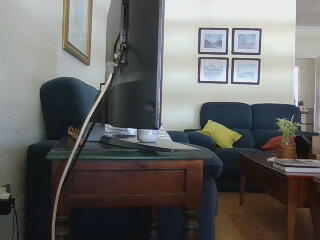
\includegraphics[width = 0.7\textwidth]{images/VideoRecibido2.1.png}
  \captionof{figure}{Vídeo recibido en \textit{Minimal\_Video} para ancho de banda de 10 Mbps.}
  \label{fig:minimal_video_10mbps}
\end{center}

\newpage

Ahora, ejecutaremos el módulo \textit{Minimal\_Video\_FPS} con el mismo ancho de banda, 10 Mbps. El comando usado ha sido el siguiente:
\begin{lstlisting}[language=bash, basicstyle=\ttfamily\scriptsize]
    python minimal_video_fps.py -a 192.168.0.58 --show_video --show_stats -z 12
\end{lstlisting}
Donde \verb|-a| es la dirección IP destino, \verb|--show_video| es para que se active la transmisión de vídeo, \verb|--show_stats| es para que se muestre la información de estadísticas y \verb|-z| es el numero de fotogramas por segundo (FPS) que se desea enviar. En este caso, se ha configurado para mostrar el vídeo a 12 FPS.

A continuación, se probará el módulo con un ancho de banda bajo, de 10 Mbps. El resultado obtenido ha sido el siguiente:
\vspace{\baselineskip}

\begin{lstlisting}[language=bash,basicstyle=\ttfamily\tiny]
         |  AUDIO (msg)  |  VIDEO (msg)  |  AUDIO (kbps)   |  VIDEO (kbps)   |     CPU (%) 
   Cycle |  Sent  Recv   |  Sent  Recv   |   Sent   Recv   |   Sent   Recv   | Program System
================================================================================================
       1 |   25    25    |  147     0    |   802    802    |  1613      0    |  22      0       
       2 |   33    10    |   18     0    |  1077    326    |   198      0    |  37     77       
       3 |   33    33    |    0     0    |  1080   1080    |     0      0    |  34     80       
       4 |   33    33    |  267   240    |  1077   1077    |  2977   2679    |  37     67       
       5 |   39    39    |  288   259    |  1232   1232    |  3106   2795    |  55     69       
       6 |   36    36    |  276   248    |  1172   1172    |  3068   2761    |  23     65
       7 |   32    32    |  243   219    |  1042   1042    |  2702   2432    |  30     69       
       8 |   33    33    |  220   198    |  1049   1049    |  2389   2150    |  35     58       
       9 |   35    35    |  198   178    |  1124   1124    |  2170   1953    |  46     67       
      10 |   31    31    |  215   194    |  1007   1007    |  2386   2147    |  26     69       
      11 |   30    30    |  266   239    |   963    963    |  2914   2623    |  35     71       
      12 |   35    35    |  284   256    |  1145   1145    |  3175   2858    |  37     80       
      13 |   32    32    |  266   239    |  1044   1044    |  2963   2667    |  31     74       
      14 |   29    29    |  186   167    |   941    941    |  2061   1855    |  30     78       
      15 |   33    33    |  184   166    |  1077   1077    |  2052   1847    |  37     80       
      16 |   34    34    |  231   208    |  1110   1110    |  2577   2319    |  26     77       
      17 |   29    29    |  201   181    |   926    926    |  2191   1972    |  22     73       
      18 |    1     1    |  132   119    |    32     32    |  1450   1305    |   4     60       
   Cycle |  Sent  Recv   |  Sent  Recv   |   Sent   Recv   |   Sent   Recv   | Program System
         |  AUDIO (msg)  |  VIDEO (msg)  |  AUDIO (kbps)   |  VIDEO (kbps)   |     CPU (%) 
===========================================================================================
Socket blocked while sending fragment 41.
Socket blocked while sending fragment 42.
Socket blocked while sending fragment 43.
Socket blocked while sending fragment 8.
Socket blocked while sending fragment 9.
Socket blocked while sending fragment 17.
Socket blocked while sending fragment 18.
Socket blocked while sending fragment 19.
Socket blocked while sending fragment 137.
Socket blocked while sending fragment 138.
Socket blocked while sending fragment 139.
Socket blocked while sending fragment 140.
Socket blocked while sending fragment 141.
Socket blocked while sending fragment 142.
Socket blocked while sending fragment 143.
Socket blocked while sending fragment 144.
Video application stopped.

=== Global bandwidth statistics ===
Audio sent:       980.18 kbps
Audio received:   939.41 kbps
Video sent:       2191.73 kbps
Video received:   1973.56 kbps
Total time:       18.5 s
=====================================

=== FPS Statistics ===
Target FPS:       12.0
Average real FPS: 1.2
FPS efficiency:   9.9%
======================
Program terminated.
QObject::killTimer: Timers cannot be stopped from another thread
QObject::~QObject: Timers cannot be stopped from another thread
\end{lstlisting}
\vspace{\baselineskip}

\newpage

La imagen de la Figura \ref{fig:minimal_video_fps_10mbps} es una captura del vídeo recibido en esta prueba.
\begin{center}
  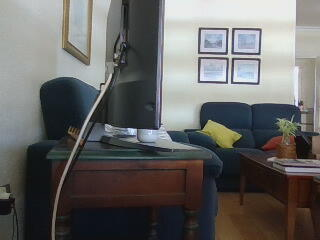
\includegraphics[width = 0.7\textwidth]{images/VideoRecibido2.2.png}
  \captionof{figure}{Vídeo recibido en \textit{Minimal\_Video\_FPS} para ancho de banda de 10 Mbps.}
  \label{fig:minimal_video_fps_10mbps}
\end{center}

\newpage

Finalmente, se ejecutará el módulo \textit{Minimal\_Video\_Resolution} con el mismo ancho de banda, 10 Mbps. El comando usado ha sido el siguiente:
\begin{lstlisting}[language=bash,basicstyle=\ttfamily\scriptsize]
python minimal_video_resolution.py -a 192.168.0.58 --show_video --show_stats -z 12 \\
-w 350 -g 250
\end{lstlisting}
Donde \verb|-a| indica la dirección IP destino, \verb|--show_video| indica que se active la transmisión de vídeo, \verb|--show_stats| indica que se muestren las estadísticas de la transmisión, \verb|-z| indica el número de fotogramas por segundo (FPS), \verb|-w| indica el ancho del vídeo y \verb|-g| indica la altura del vídeo.
\vspace{\baselineskip}

\begin{lstlisting}[language=bash,basicstyle=\ttfamily\tiny]
         |  AUDIO (msg)  |  VIDEO (msg)  |  AUDIO (kbps)   |  VIDEO (kbps)   |     CPU (%) 
   Cycle |  Sent  Recv   |  Sent  Recv   |   Sent   Recv   |   Sent   Recv   | Program System
================================================================================================
       1 |   27    27    |  188   188    |   882    882    |  2098   2098    |  17      0       
       2 |   37    37    |    0     0    |  1150   1150    |     0      0    |  35     76       
       3 |   29    29    |  188   188    |   939    939    |  2079   2081    |  31     78       
       4 |   31    31    |  937   882    |  1014   1014    | 10470   9853    |  22     73       
   Cycle |  Sent  Recv   |  Sent  Recv   |   Sent   Recv   |   Sent   Recv   | Program System
         |  AUDIO (msg)  |  VIDEO (msg)  |  AUDIO (kbps)   |  VIDEO (kbps)   |     CPU (%) 
===========================================================================================
Socket blocked while sending fragment 64.
Socket blocked while sending fragment 65.
Socket blocked while sending fragment 66.
Socket blocked while sending fragment 67.
Socket blocked while sending fragment 71.
Socket blocked while sending fragment 72.
Socket blocked while sending fragment 73.
Socket blocked while sending fragment 84.
Socket blocked while sending fragment 85.
Socket blocked while sending fragment 136.
Socket blocked while sending fragment 137.
Socket blocked while sending fragment 138.
Socket blocked while sending fragment 139.
Socket blocked while sending fragment 140.
Socket blocked while sending fragment 141.
Socket blocked while sending fragment 142.
Socket blocked while sending fragment 143.
Socket blocked while sending fragment 144.
Socket blocked while sending fragment 145.
Socket blocked while sending fragment 146.
Socket blocked while sending fragment 147.
Socket blocked while sending fragment 148.
Socket blocked while sending fragment 149.
Socket blocked while sending fragment 150.
Socket blocked while sending fragment 151.
Socket blocked while sending fragment 152.
Socket blocked while sending fragment 153.
Socket blocked while sending fragment 154.
Socket blocked while sending fragment 155.
       5 |   35    35    |  848   786    |  1144   1144    |  9466   8773    |  24     73       
   Cycle |  Sent  Recv   |  Sent  Recv   |   Sent   Recv   |   Sent   Recv   | Program System
         |  AUDIO (msg)  |  VIDEO (msg)  |  AUDIO (kbps)   |  VIDEO (kbps)   |     CPU (%) 
===========================================================================================
Socket blocked while sending fragment 185.
Socket blocked while sending fragment 93.
Socket blocked while sending fragment 94.
Socket blocked while sending fragment 95.
Socket blocked while sending fragment 96.
Socket blocked while sending fragment 97.
Socket blocked while sending fragment 118.
Socket blocked while sending fragment 119.
Socket blocked while sending fragment 120.
Socket blocked while sending fragment 121.
Socket blocked while sending fragment 122.
Socket blocked while sending fragment 123.
Socket blocked while sending fragment 124.
Socket blocked while sending fragment 125.
Socket blocked while sending fragment 12.
Socket blocked while sending fragment 73.
Socket blocked while sending fragment 75.
Socket blocked while sending fragment 76.
Socket blocked while sending fragment 79.
Socket blocked while sending fragment 81.
Socket blocked while sending fragment 82.
Socket blocked while sending fragment 83.
Socket blocked while sending fragment 88.
Socket blocked while sending fragment 71.
Socket blocked while sending fragment 97.
Socket blocked while sending fragment 115.
Socket blocked while sending fragment 116.
Socket blocked while sending fragment 117.
Socket blocked while sending fragment 118.
       6 |   34    34    |  801   732    |  1067   1067    |  8582   7842    |  24     73       
   Cycle |  Sent  Recv   |  Sent  Recv   |   Sent   Recv   |   Sent   Recv   | Program System
         |  AUDIO (msg)  |  VIDEO (msg)  |  AUDIO (kbps)   |  VIDEO (kbps)   |     CPU (%) 
===========================================================================================
Socket blocked while sending fragment 137.
Socket blocked while sending fragment 138.
Socket blocked while sending fragment 139.
Socket blocked while sending fragment 140.
Socket blocked while sending fragment 141.
Socket blocked while sending fragment 142.
Socket blocked while sending fragment 143.
Socket blocked while sending fragment 144.
Socket blocked while sending fragment 178.
Socket blocked while sending fragment 187.
Socket blocked while sending fragment 29.
Socket blocked while sending fragment 30.
Socket blocked while sending fragment 31.
Socket blocked while sending fragment 32.
Socket blocked while sending fragment 33.
Socket blocked while sending fragment 34.
Socket blocked while sending fragment 35.
Socket blocked while sending fragment 36.
Socket blocked while sending fragment 37.
Socket blocked while sending fragment 38.
Socket blocked while sending fragment 39.
Socket blocked while sending fragment 175.
Socket blocked while sending fragment 184.
Socket blocked while sending fragment 185.
Socket blocked while sending fragment 24.
Socket blocked while sending fragment 25.
Socket blocked while sending fragment 26.
Socket blocked while sending fragment 27.
Socket blocked while sending fragment 28.
Socket blocked while sending fragment 29.
       7 |   32    32    |  868   801    |  1003   1003    |  9295   8577    |  25     72       
   Cycle |  Sent  Recv   |  Sent  Recv   |   Sent   Recv   |   Sent   Recv   | Program System
         |  AUDIO (msg)  |  VIDEO (msg)  |  AUDIO (kbps)   |  VIDEO (kbps)   |     CPU (%) 
===========================================================================================
Socket blocked while sending fragment 89.
Socket blocked while sending fragment 90.
Socket blocked while sending fragment 180.
Socket blocked while sending fragment 181.
Socket blocked while sending fragment 182.
Socket blocked while sending fragment 183.
Socket blocked while sending fragment 184.
Socket blocked while sending fragment 185.
Socket blocked while sending fragment 186.
Socket blocked while sending fragment 187.
Socket blocked while sending fragment 29.
^CSocket blocked while sending fragment 47.
Socket blocked while sending fragment 49.
Socket blocked while sending fragment 62.
Socket blocked while sending fragment 63.
Socket blocked while sending fragment 73.
Socket blocked while sending fragment 74.
Socket blocked while sending fragment 46.
Socket blocked while sending fragment 47.
Socket blocked while sending fragment 48.
Socket blocked while sending fragment 49.
Socket blocked while sending fragment 50.
       8 |    7     7    |  491   442    |   228    228    |  5469   4925    |   8     61       
   Cycle |  Sent  Recv   |  Sent  Recv   |   Sent   Recv   |   Sent   Recv   | Program System
         |  AUDIO (msg)  |  VIDEO (msg)  |  AUDIO (kbps)   |  VIDEO (kbps)   |     CPU (%) 
===========================================================================================
Video application stopped.

=== Global bandwidth statistics ===
Audio sent:       546.99 kbps
Audio received:   546.99 kbps
Video sent:       3477.81 kbps
Video received:   3234.63 kbps
Total time:       13.9 s
=====================================

=== FPS Statistics ===
Target FPS:       12.0
Average real FPS: 1.6
FPS efficiency:   13.7%
======================

=== Resolution Statistics ===
Target resolution: 350x250
Actual resolution: 352x288
Average rescaling time: 6.47 ms
Performance impact:     7.8%
=============================

=== Camera compatible resolutions ===
  1. 320x240
  2. 352x288 * SELECTED
  3. 640x360
  4. 640x480
  5. 800x600
  6. 1024x768
  7. 1280x720
  8. 1280x1024
  9. 1366x768
  10. 1600x900
  11. 1920x1080
  12. 2560x1440
  13. 3840x2160

Camera device: /dev/video0
======================================
Program terminated.
QObject::killTimer: Timers cannot be stopped from another thread
QObject::~QObject: Timers cannot be stopped from another thread
\end{lstlisting}
\vspace{\baselineskip}

La imagen de la Figura \ref{fig:minimal_video_resolution_10mbps} es una captura del vídeo recibido en esta prueba.
\begin{center}
  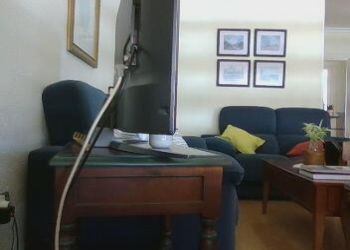
\includegraphics[width = 0.7\textwidth]{images/VideoRecibido2.3.png}
  \captionof{figure}{Vídeo recibido en \textit{Minimal\_Video\_Resolution} para ancho de banda de 10 Mbps.}
  \label{fig:minimal_video_resolution_10mbps}
\end{center}
\newpage

Ahora, se procederá a extraer las conclusiones correspondientes a las pruebas realizadas con un ancho de banda bajo, 10 Mbps.
\vspace{\baselineskip}

\textbf{Análisis de \textit{Minimal\_Video} con 10 Mbps de tasa de transferencia:}
\vspace{\baselineskip}

El comportamiento de \textit{Minimal\_Video} bajo el límite del ancho de banda de 10 Mbps mejora notablemente respecto a la prueba de 1 Mbps. Según las estadísticas globales, el módulo intentó enviar 5481.62 kbps de vídeo y 860.65 kbps de audio, logrando recibir 4927.59 kbps de vídeo y 798.34 kbps de audio. Esto indica que la mayor parte de los datos logra transmitirse correctamente, y la experiencia del usuario es considerablemente mejor: el vídeo y el audio son reconocibles y, en general, la comunicación es funcional.
\vspace{\baselineskip}

Sin embargo, la presencia de mensajes como ``Socket bloqueado al enviar fragmento X'' (por ejemplo, entre el ciclo 4 y 5, y entre el ciclo 5 y 6) indica que el módulo sigue generando picos de tráfico o un flujo sostenido que, en ocasiones, sobrepasa la capacidad de la red. En dichos ciclos, el socket bloquea temporalmente el envío de nuevos paquetes hasta aliviar la congestión en la cola de red. Es cierto que los fotogramas individuales que logran transmitirse pueden mantener una buena calidad visual, como se observa en la Figura \ref{fig:minimal_video_fps_10mbps}, estos bloqueos pueden resultar en una experiencia visual con interrupciones momentáneas en la fluidez o la aparición de artefactos leves que no son evidentes en cada fotograma individual capturado. El sistema funciona y la comunicación es reconocible, pero la fluidez no es perfectamente constante y aún existen limitaciones para un uso completamente estable.

\vspace{\baselineskip}

\textbf{Análisis de \textit{Minimal\_Video\_FPS} con 10 Mbps de tasa de transferencia:}
\vspace{\baselineskip}

Al aumentar el ancho de banda a 10 Mbps, este módulo, que intenta fijar la tasa de FPS en 12, muestra un resultado significativamente mejorado. Las estadísticas globales indican un envío de 980.18 kbps de audio (con 939.41 kbps recibidos), lo cual es positivo para el audio. Para el vídeo, se intentaron enviar 2191.73 kbps y se recibieron 1973.56 kbps, representando una eficiencia de transmisión del 90\%. Siguen apareciendo mensajes de ``Socket bloqueado'', lo que indica que el módulo sigue enfrentando congestión en la red, pero en menor medida que con 1 Mbps.
\vspace{\baselineskip}

La sección de ``Estadísticas de FPS'' revela que, pese a tener de objetivo 12 FPS, solo se logra un promedio real de 1.2 FPS (eficiencia del 9.9\%). Sin embargo, a diferencia de la situación anterior, ahora existe una recepción exitosa del 90\% del vídeo transmitido. Esta aparente contradicción entre el bajo FPS real (1.2) y la alta eficiencia de transmisión de vídeo (90\%) sugiere que el sistema logra transmitir los fotogramas de vídeo de manera efectiva cuando los genera, pero la limitación principal radica en la capacidad de generación/captura de fotogramas por parte del módulo. La visualización del vídeo es funcional en este caso, aunque con una tasa de fotogramas considerablemente inferior a la deseada, lo que indica que el cuello de botella se encuentra en el procesamiento local más que en la capacidad de la red con 10 Mbps.

\vspace{\baselineskip}

\textbf{Análisis de \textit{Minimal\_Video\_Resolution} con 10 Mbps de tasa de transferencia:}
\vspace{\baselineskip}

En este caso, el módulo intenta transmitir vídeo a 12 FPS y una resolución objetivo de 350x250 píxeles (ajustando realmente a 352x288, que es la resolución compatible según la cámara). Los datos globales muestran que se enviaron 3477.81 kbps de vídeo (con 3234.63 kbps recibidos) y 546.99 kbps de audio (recibidos en su totalidad). La recepción de vídeo y audio es considerable, lo que es una mejora respecto al módulo \textit{Minimal\_Video\_FPS}.
\vspace{\baselineskip}

Las ``Estadísticas de FPS'' indican un promedio real de 1.6 FPS frente al objetivo de 12 (eficiencia del 13.7\%). Aunque se recibe vídeo y los fotogramas individuales pueden mostrar una calidad visual aceptable como se aprecia en la Figura \ref{fig:minimal_video_resolution_10mbps}, la eficiencia de FPS es baja. Esto resulta en una experiencia de vídeo con una fluidez muy limitada y una percepción de movimiento entrecortada, ya que la tasa de actualización de la imagen es significativamente inferior a la deseada.  Los mensajes de ``Socket bloqueado'' (visibles entre los ciclos 4 y 5, 5 y 6, etc.) confirman esta congestión. El tiempo de reescalado promedio es de 6.47 ms, con un impacto en CPU del 7.8\%, lo cual es manejable. El sistema transmite vídeo y audio, pero la fluidez es muy pobre debido la limitación de la red para sostener 12 FPS.
\vspace{\baselineskip}

\textbf{Conclusiones para limitación 10 Mbps de tasa de transferencia:}

La ejecución de los módulos con un ancho de banda de 10 Mbps muestra resultados mixtos, con una mejora general respecto a 1 Mbps, pero con problemas significativos en algunos escenarios.
\begin{itemize}
\item \textbf{Transmisión variable según el módulo:} \textit{Minimal\_Video} y \textit{Minimal\_Video\_Resolution} logran transmitir una cantidad sustancial de datos de vídeo y audio (vídeo recibido: 4927.59 kbps y 3234.63 kbps respectivamente), permitiendo una comunicación reconocible. \textit{Minimal\_Video\_FPS} logra una transmisión de vídeo parcialmente efectiva (1973.56 kbps recibidos de 2191.73 kbps enviados, 90\% de eficiencia) pero con limitaciones en la generación de fotogramas.
\item \textbf{Congestión:} A pesar del aumento de ancho de banda, los mensajes de ``Socket bloqueado'' siguen apareciendo en todos los módulos. La baja eficiencia de FPS en los módulos que lo gestionan (9.9\% para \textit{Minimal\_Video\_FPS} y 13.7\% para \textit{Minimal\_Video\_Resolution}, con FPS reales de 1.2 y 1.6 respectivamente) indica que el cuello de botella principal no radica en la capacidad de red sino en el procesamiento local y la generación de fotogramas. Para \textit{Minimal\_Video\_FPS}, la red de 10 Mbps es capaz de transmitir eficientemente el vídeo generado, pero la baja tasa de generación limita la experiencia.
\item \textbf{Impacto de funcionalidades avanzadas:} El intento de fijar FPS en \textit{Minimal\_Video\_FPS} revela una separación clara entre la capacidad de transmisión de red (exitosa al 90\%) y la capacidad de generación de fotogramas (limitada al 9.9\% de eficiencia). \textit{Minimal\_Video\_Resolution}, aunque con FPS bajos, gestiona mejor tanto la generación como la transmisión. El coste de CPU del reescalado en \textit{Minimal\_Video\_Resolution} (7.8\%) es moderado.
\item \textbf{Mejora pequeña en rendimiento:} Mientras que \textit{Minimal\_Video} ofrece una experiencia básica funcional, los módulos que intentan controlar los FPS muestran que el principal desafío no es el ancho de banda de 10 Mbps sino la optimización del procesamiento local. \textit{Minimal\_Video\_FPS} demuestra que la red puede transmitir efectivamente el vídeo cuando está disponible, pero la generación de fotogramas a 12 FPS requiere optimizaciones en el procesamiento de vídeo local más que un mayor ancho de banda.
\end{itemize}

\newpage

\textbf{Pruebas de limitación de la tasa de transferencia a 50 Mbps}
\vspace{\baselineskip}

Empezaremos por probar el módulo con un ancho de banda alto, 50 Mbps. El comando usado para \textit{Minimal\_Video} ha sido el siguiente:

\begin{lstlisting}[language=bash]
python minimal_video.py -a 192.168.0.58 --show_video --show_stats
\end{lstlisting}
Donde \verb|-a| es la dirección IP del dispositivo con el que se va a comunicar el módulo, \verb|--show_video| es la opción para mostrar el vídeo en tiempo real y \verb|--show_stats| es la opción para mostrar las estadísticas de la red.
\vspace{\baselineskip}

\begin{lstlisting}[language=bash,basicstyle=\ttfamily\tiny]
         |  AUDIO (msg)  |  VIDEO (msg)  |  AUDIO (kbps)   |  VIDEO (kbps)   |     CPU (%) 
   Cycle |  Sent  Recv   |  Sent  Recv   |   Sent   Recv   |   Sent   Recv   | Program System
================================================================================================
       1 |   29    29    |  165   153    |   949    949    |  1845   1713    |  16      0       
       2 |   35    35    |    0     0    |  1121   1121    |     0      0    |  45     78       
       3 |   31    31    |  464   463    |  1008   1008    |  5152   5137    |  40     71       
       4 |   29    29    |  975   912    |   946    946    | 10861  10161    |  23     76       
       5 |   26    26    |  865   747    |   845    845    |  9600   8291    |  36     66       
       6 |   33    33    | 1231  1143    |  1080   1080    | 13759  12772    |  48     74       
       7 |   39    39    |  444   313    |  1241   1241    |  4823   3402    |  49     72       
       8 |   37    37    | 1129  1094    |  1164   1164    | 12125  11749    |  41     75       
       9 |   29    29    | 1250  1186    |   948    948    | 13957  13240    |  31     78       
      10 |   42    42    |  924   790    |  1371   1371    | 10296   8803    |  36     67       
      11 |   37    22    |  717   582    |  1203    715    |  7961   6462    |  43     71       
      12 |   29    29    | 1068  1004    |   948    948    | 11922  11209    |  31     69       
      13 |   28    28    |  990   980    |   916    916    | 11058  10948    |  33     73       
      14 |   15    15    |  818   787    |   489    489    |  9117   8769    |  23     72       
   Cycle |  Sent  Recv   |  Sent  Recv   |   Sent   Recv   |   Sent   Recv   | Program System
         |  AUDIO (msg)  |  VIDEO (msg)  |  AUDIO (kbps)   |  VIDEO (kbps)   |     CPU (%) 
===========================================================================================
Video application stopped.

=== Global bandwidth statistics ===
Audio sent:       1000.25 kbps
Audio received:   966.08 kbps
Video sent:       8587.79 kbps
Video received:   7898.40 kbps
Total time:       14.4 s
=====================================
Program terminated.
QObject::killTimer: Timers cannot be stopped from another thread
QObject::~QObject: Timers cannot be stopped from another thread
\end{lstlisting}
\vspace{\baselineskip}

\newpage

La imagen de la Figura \ref{fig:minimal_video_50mbps} es una captura del vídeo recibido en esta prueba.
\begin{center}
  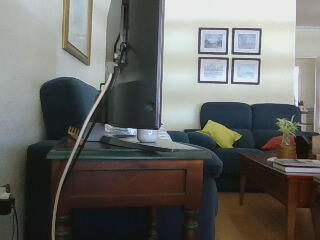
\includegraphics[width = 0.7\textwidth]{images/VideoRecibido3.1.png}
  \captionof{figure}{Vídeo recibido en \textit{Minimal\_Video} para ancho de banda de 50 Mbps.}
  \label{fig:minimal_video_50mbps}
\end{center}

\newpage
Ahora, ejecutaremos el módulo \textit{Minimal\_Video\_FPS} con el mismo ancho de banda, 50 Mbps. El comando usado ha sido el siguiente:
\begin{lstlisting}[language=bash, basicstyle=\ttfamily\scriptsize]
    python minimal_video_fps.py -a 192.168.0.58 --show_video --show_stats -z 12
\end{lstlisting}
Donde \verb|-a| es la dirección IP destino, \verb|--show_video| es para que se active la transmisión de vídeo, \verb|--show_stats| es para que se muestre la información de estadísticas y \verb|-z| es el numero de fotogramas por segundo (FPS) que se desea enviar. En este caso, se ha configurado para mostrar el vídeo a 12 FPS.
\vspace{\baselineskip}

\begin{lstlisting}[language=bash,basicstyle=\ttfamily\tiny]
         |  AUDIO (msg)  |  VIDEO (msg)  |  AUDIO (kbps)   |  VIDEO (kbps)   |     CPU (%) 
   Cycle |  Sent  Recv   |  Sent  Recv   |   Sent   Recv   |   Sent   Recv   | Program System
================================================================================================
       1 |   20    20    |  165   165    |   651    651    |  1836   1836    |  24      0       
       2 |   34    34    |  332   330    |   957    957    |  3191   3172    |  30     76       
       3 |   26    26    |  946   901    |   850    850    | 10564  10059    |  24     72       
       4 |   39    36    |  557   330    |  1243   1147    |  6059   3590    |  38     63       
       5 |   28    28    | 1077   997    |   915    915    | 12016  11123    |  28     71       
       6 |   31    31    | 1142  1112    |  1014   1014    | 12752  12419    |  45     74       
       7 |   35    35    |  940   922    |  1140   1140    | 10458  10257    |  34     73       
       8 |   38    25    |  391   199    |  1243    817    |  4367   2220    |  45     66       
       9 |   30    24    |  718   641    |   980    784    |  8006   7151    |  43     75       
      10 |   25    25    |  825   825    |   818    818    |  9221   9221    |  38     78       
      11 |   37    37    | 1155  1141    |  1207   1207    | 12871  12719    |  43     75       
      12 |   31    31    |  825   810    |  1014   1014    |  9219   9051    |  32     76       
      13 |   28    28    |  825   825    |   912    912    |  9181   9181    |  30     70       
   Cycle |  Sent  Recv   |  Sent  Recv   |   Sent   Recv   |   Sent   Recv   | Program System
         |  AUDIO (msg)  |  VIDEO (msg)  |  AUDIO (kbps)   |  VIDEO (kbps)   |     CPU (%) 
===========================================================================================
Video application stopped.

=== Global bandwidth statistics ===
Audio sent:       976.67 kbps
Audio received:   923.22 kbps
Video sent:       8209.75 kbps
Video received:   7629.43 kbps
Total time:       13.5 s
=====================================

=== FPS Statistics ===
Target FPS:       12.0
Average real FPS: 5.0
FPS efficiency:   41.5%
======================
Program terminated.
QObject::killTimer: Timers cannot be stopped from another thread
QObject::~QObject: Timers cannot be stopped from another thread
\end{lstlisting}
\vspace{\baselineskip}

\newpage

La imagen de la Figura \ref{fig:minimal_video_fps_50mbps} es una captura del vídeo recibido en esta prueba.
\begin{center}
  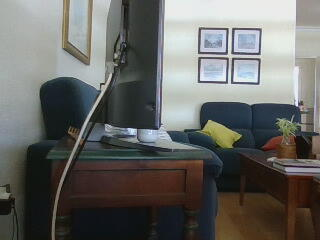
\includegraphics[width = 0.7\textwidth]{images/VideoRecibido3.2.png}
  \captionof{figure}{Vídeo recibido en \textit{Minimal\_Video\_FPS} para ancho de banda de 50 Mbps.}
  \label{fig:minimal_video_fps_50mbps}
\end{center}

\newpage
Finalmente, se ejecutará el módulo \textit{Minimal\_Video\_Resolution} con el mismo ancho de banda, 50 Mbps. El comando usado ha sido el siguiente:

\begin{lstlisting}[language=bash,basicstyle=\ttfamily\scriptsize]
python minimal_video_resolution.py -a 192.168.0.58 --show_video --show_stats -z 12 \\
-w 350 -g 250
\end{lstlisting}
Donde \verb|-a| indica la dirección IP destino, \verb|--show_video| indica que se active la transmisión de vídeo, \verb|--show_stats| indica que se muestren las estadísticas de la transmisión, \verb|-z| indica el número de fotogramas por segundo (FPS), \verb|-w| indica el ancho del vídeo y \verb|-g| indica la altura del vídeo.
\vspace{\baselineskip}

\begin{lstlisting}[language=bash,basicstyle=\ttfamily\tiny]
         |  AUDIO (msg)  |  VIDEO (msg)  |  AUDIO (kbps)   |  VIDEO (kbps)   |     CPU (%) 
   Cycle |  Sent  Recv   |  Sent  Recv   |   Sent   Recv   |   Sent   Recv   | Program System
================================================================================================
       1 |   32    32    |  188   186    |  1042   1042    |  2091   2071    |  26      0       
       2 |   36    36    |  259   211    |  1166   1166    |  2865   2331    |  34     70       
       3 |   29    29    | 1055  1032    |   946    946    | 11757  11503    |  34     72       
       4 |   31    31    |  967   924    |  1003   1003    | 10686  10212    |  30     71       
       5 |   25    25    | 1190  1184    |   798    798    | 12976  12907    |  35     77       
       6 |   28    28    | 1052  1044    |   916    916    | 11755  11666    |  34     71       
       7 |   35    35    |  827   688    |  1144   1144    |  9235   7681    |  38     71       
       8 |   21    21    |  784   727    |   684    684    |  8720   8087    |  14     78       
       9 |   34    34    |  996   951    |  1111   1111    | 11113  10607    |  43     69       
      10 |   30    30    | 1018  1019    |   981    981    | 11363  11377    |  31     71       
      11 |   29    29    | 1085  1010    |   949    949    | 12127  11288    |  36     73       
      12 |   30    30    |  878   862    |   980    980    |  9801   9620    |  24     73       
      13 |   31    31    |  929   866    |  1004   1004    | 10280   9584    |  32     74       
      14 |   31    11    |  228     0    |  1014    360    |  2548      0    |  42     65       
      15 |   30     0    |  200     0    |   982      0    |  2233      0    |  45     63       
      16 |   31     0    |  201     0    |  1004      0    |  2222      0    |  45     67       
      17 |    0     0    |  175     0    |     0      0    |  1932      0    |   2     12       
   Cycle |  Sent  Recv   |  Sent  Recv   |   Sent   Recv   |   Sent   Recv   | Program System
         |  AUDIO (msg)  |  VIDEO (msg)  |  AUDIO (kbps)   |  VIDEO (kbps)   |     CPU (%) 
===========================================================================================
Video application stopped.

=== Global bandwidth statistics ===
Audio sent:       904.14 kbps
Audio received:   752.51 kbps
Video sent:       7688.82 kbps
Video received:   6840.18 kbps
Total time:       17.5 s
=====================================

=== FPS Statistics ===
Target FPS:       12.0
Average real FPS: 3.6
FPS efficiency:   29.8%
======================

=== Resolution Statistics ===
Target resolution: 350x250
Actual resolution: 352x288
Average rescaling time: 5.53 ms
Performance impact:     6.6%
=============================

=== Camera compatible resolutions ===
  1. 320x240
  2. 352x288 * SELECTED
  3. 640x360
  4. 640x480
  5. 800x600
  6. 1024x768
  7. 1280x720
  8. 1280x1024
  9. 1366x768
  10. 1600x900
  11. 1920x1080
  12. 2560x1440
  13. 3840x2160

Camera device: /dev/video0
======================================
Program terminated.
QObject::killTimer: Timers cannot be stopped from another thread
QObject::~QObject: Timers cannot be stopped from another thread
\end{lstlisting}
\vspace{\baselineskip}

\newpage
La imagen de la Figura \ref{fig:minimal_video_resolution_50mbps} es una captura del vídeo recibido en esta prueba.
\begin{center}
  
\includegraphics[width = 0.7\textwidth]{images/VideoRecibido3.3.png}
  \captionof{figure}{Vídeo recibido en \textit{Minimal\_Video\_Resolution} para ancho de banda de 50 Mbps.}
  \label{fig:minimal_video_resolution_50mbps}
\end{center}

\newpage

Ahora, se procederá a extraer las conclusiones correspondientes a las pruebas realizadas con un ancho de banda alto, 50 Mbps.
\vspace{\baselineskip}

\textbf{Análisis de \textit{Minimal\_Video} con 50 Mbps de tasa de transferencia:}
\vspace{\baselineskip}

Al examinar el comportamiento de \textit{Minimal\_Video} bajo esta condición de red de 50 Mbps, se observa una mejora muy significativa respecto a las pruebas con anchos de banda inferiores. Las estadísticas globales muestran que el módulo intentó enviar 8587.79 kbps de vídeo y 1000.25 kbps de audio, logrando recibir 7898.40 kbps de vídeo y 966.08 kbps de audio. Estos valores representan un porcentaje de recepción muy alto (aproximadamente el 92.0\% para vídeo y 96.6\% para audio), lo que indica que el ancho de banda disponible es bien aprovechado y suficiente para la carga generada.
\vspace{\baselineskip}

Es importante destacar que en la salida proporcionada no se observan mensajes de ``Socket bloqueado'', lo que confirma que la red puede manejar adecuadamente el flujo de datos generado por el módulo sin llegar a la congestión. La experiencia del usuario mejora notablemente: el vídeo se muestra fluido y el audio se escucha claro y continuo. Dado que este módulo no implementa un control específico de FPS (por defecto estará establecido a 30 FPS), la tasa de fotogramas variará según la carga del sistema y la capacidad de la cámara, pero la transmisión de los fotogramas generados es eficiente.

\vspace{\baselineskip}

\textbf{Análisis de \textit{Minimal\_Video\_FPS} con 50 Mbps de tasa de transferencia:}
\vspace{\baselineskip}

Este módulo, que intenta obtener una tasa de fotogramas de 12 FPS, muestra un comportamiento considerablemente mejorado con 50 Mbps. Los datos globales indican un envío de 8209.75 kbps de vídeo (con 7629.43 kbps recibidos) y 976.67 kbps de audio (con 923.22 kbps recibidos). El porcentaje de recepción es alto (aproximadamente 92.9\% para vídeo y 94.5\% para audio), lo que sugiere que el ancho de banda es en su mayor parte adecuado.
\vspace{\baselineskip}

La sección de ``Estadísticas de FPS'' revela que el módulo alcanza un promedio real de 5.0 FPS frente al objetivo de 12 FPS, lo que representa una eficiencia del 41.5\%. Aunque esto supone una mejora sustancial respecto a las pruebas con anchos de banda más limitados y permite una experiencia visual más fluida, todavía no se alcanza el objetivo. Este rendimiento sugiere que, incluso con un ancho de banda amplio, pueden existir otros factores limitantes (posiblemente relacionados con el procesamiento necesario para capturar, codificar y enviar a 12 FPS) que impiden alcanzar la tasa objetivo de forma consistente. Sin embargo, la experiencia del usuario es significativamente mejor, con un vídeo más estable.

\vspace{\baselineskip}

\textbf{Análisis de \textit{Minimal\_Video\_Resolution} con 50 Mbps de tasa de transferencia:}
\vspace{\baselineskip}

Este módulo, que combina el control de FPS a 12 con una resolución objetivo de 350x250 (ajustada a la compatible 352x288), muestra un rendimiento aceptable con 50 Mbps, aunque con algunas particularidades. Las estadísticas globales indican un envío de 7688.82 kbps de vídeo y 904.14 kbps de audio. De estos, se recibieron 6840.18 kbps de vídeo y 752.51 kbps de audio. Es importante señalar que los últimos ciclos de la prueba (del ciclo 14 al 17) muestran una recepción de 0 kbps tanto para audio como para vídeo, lo que indica una interrupción o fallo en la comunicación hacia el final de la prueba. Si excluimos estos ciclos finales problemáticos, la recepción en los ciclos anteriores fue muy buena.

Las ``Estadísticas de FPS'' muestran que se logran 3.6 FPS reales de los 12 FPS objetivo (eficiencia del 29.8\%). Este valor es inferior al del módulo \textit{Minimal\_Video\_FPS}, y también se ve afectado por la interrupción final. El ``Tiempo de reescalado promedio'' es de 5.53 ms, con un impacto en el rendimiento (CPU) del 6.6\%. Este coste de procesamiento es moderado. La resolución real utilizada es 352x288. La interrupción en la recepción al final de la prueba afecta negativamente la percepción de fiabilidad, aunque durante la mayor parte de la ejecución la transmisión fue buena.
\vspace{\baselineskip}

\textbf{Conclusiones para limitación 50 Mbps:}

La ejecución de los módulos con un ancho de banda de 50 Mbps muestra un rendimiento significativamente superior, acercándose a una experiencia de comunicación de vídeo y audio de buena calidad, aunque persisten algunas limitaciones.
\begin{itemize}
\item \textbf{Transmisión mayoritariamente exitosa y sin congestión de red:} Para los módulos, concretamente, \textit{Minimal\_Video} y \textit{Minimal\_Video\_FPS}, la gran mayoría de los datos enviados son recibidos correctamente (tasas de recepción de vídeo superiores al 92\%). Los mensajes de ``Socket bloqueado'' no aparecen, indicando que la red de 50 Mbps maneja adecuadamente el flujo de datos generado. \textit{Minimal\_Video\_Resolution} también muestra buena recepción durante la mayor parte de la prueba, pero sufre una interrupción en la recepción de datos al final.
\item \textbf{Mejora en la eficacia del control de FPS, pero sin alcanzar el objetivo:} El módulo \textit{Minimal\_Video\_FPS} alcanza una eficiencia del 41.5\% (5.0 FPS reales), y \textit{Minimal\_Video\_Resolution} un 29.8\% (3.6 FPS reales). Aunque es una mejora considerable que se traduce en un vídeo más fluido, el objetivo de 12 FPS no se cumple, sugiriendo cuellos de botella más allá del ancho de banda de red (posiblemente procesamiento o limitaciones de la aplicación).
\item \textbf{Viabilidad del reescalado de resolución con impacto moderado:} Con 50 Mbps, el reescalado a 352x288 es viable, con un impacto en CPU del 6.6\% para \textit{Minimal\_Video\_Resolution}, lo cual es aceptable.
\item \textbf{Estabilidad y factores limitantes adicionales:} \textit{Minimal\_Video} es el más estable en términos de transmisión pura. Los módulos con control de FPS es cierto que mejoran per no logran el máximo rendimiento, lo que apunta a la necesidad de optimizar la aplicación o considerar las limitaciones de hardware/procesamiento para alcanzar tasas de fotogramas más altas. 
\end{itemize}

Esta prueba demuestra que un ancho de banda de 50 Mbps es suficiente para una experiencia de videollamada de buena calidad, especialmente con el módulo base. Para los módulos con control de FPS, aunque la calidad mejora sustancialmente, el no alcanzar el objetivo de 12 FPS sugiere que otros factores además del ancho de banda de red entran en juego.
\newpage

\subsubsection{Experimentos con jitter}

En esta sección, se analizarán los resultados obtenidos al aplicar una limitación de latencia (delay) a los distintos módulos.

\begin{itemize}
    \item \textbf{Pruebas con jitter)}
\end{itemize}

\textbf{Pruebas con jitter mínimo (Latencia ideal de 0 ms)}
\vspace{\baselineskip}

Comenzamos probando con una latencia ideal de 0 ms, lo que implica un jitter mínimo o despreciable, inherente a la red local.

- El comando usado para \textit{Minimal\_Video} ha sido el siguiente:
\vspace{\baselineskip}

\begin{lstlisting}[language=bash]
python minimal_video.py -a 192.168.0.58 --show_video --show_stats
\end{lstlisting}
Donde \verb|-a| es la dirección IP del dispositivo con el que se va a comunicar el módulo, \verb|--show_video| es la opción para mostrar el vídeo en tiempo real y \verb|--show_stats| es la opción para mostrar las estadísticas de la red.
\vspace{\baselineskip}

\begin{lstlisting}[language=bash,basicstyle=\ttfamily\tiny]
         |  AUDIO (msg)  |  VIDEO (msg)  |  AUDIO (kbps)   |  VIDEO (kbps)   |     CPU (%) 
   Cycle |  Sent  Recv   |  Sent  Recv   |   Sent   Recv   |   Sent   Recv   | Program System
================================================================================================
       1 |   29     0    |  165   136    |   947      0    |  1841   1519    |  26      0       
       2 |   38    33    |    0     0    |  1244   1080    |     0      0    |  44     79       
       3 |   30    30    |  237   210    |   979    979    |  2642   2339    |  39     73       
       4 |   33    33    |  688   665    |  1064   1064    |  7578   7325    |  36     77       
       5 |   26    26    | 1198  1141    |   847    847    | 13332  12699    |  36     74       
       6 |   23    23    |  601   592    |   744    744    |  6643   6541    |  22     77       
       7 |   33    33    |  613   572    |  1078   1078    |  6837   6379    |  41     75       
       8 |   26    26    | 1097  1085    |   849    849    | 12235  12101    |  27     77       
       9 |   28    28    |  917   910    |   914    914    | 10220  10142    |  24     73       
      10 |   26    26    | 1101  1075    |   813    813    | 11757  11479    |  30     73       
      11 |   32    32    |  607   557    |   993    993    |  6435   5903    |  27     77       
      12 |   28    28    |  369   368    |   895    895    |  4028   4020    |  32     78       
      13 |    9     9    |  301   302    |   293    293    |  3355   3368    |  15     68       
   Cycle |  Sent  Recv   |  Sent  Recv   |   Sent   Recv   |   Sent   Recv   | Program System
         |  AUDIO (msg)  |  VIDEO (msg)  |  AUDIO (kbps)   |  VIDEO (kbps)   |     CPU (%) 
===========================================================================================
Video application stopped.

=== Global bandwidth statistics ===
Audio sent:       882.48 kbps
Audio received:   799.36 kbps
Video sent:       6587.96 kbps
Video received:   6353.34 kbps
Total time:       13.4 s
=====================================
Program terminated.
QObject::killTimer: Timers cannot be stopped from another thread
QObject::~QObject: Timers cannot be stopped from another thread
\end{lstlisting}
\vspace{\baselineskip}

\newpage
La imagen de la Figura \ref{fig:minimal_video_0ms} es una captura del vídeo recibido en esta prueba.
\begin{center}
  
\includegraphics[width = 0.7\textwidth]{images/VideoRecibido4.1.png}
  \captionof{figure}{Vídeo recibido en \textit{Minimal\_Video} con latencia base de 0 ms.}
  \label{fig:minimal_video}
\end{center}

\newpage

Ahora, ejecutaremos el módulo \textit{Minimal\_Video\_FPS} con la misma latencia base de 0 ms y, por tanto, jitter mínimo. El comando usado ha sido el siguiente:

\begin{lstlisting}[language=bash, basicstyle=\ttfamily\scriptsize]
    python minimal_video_fps.py -a 192.168.0.58 --show_video --show_stats -z 12
\end{lstlisting}
Donde \verb|-a| es la dirección IP destino, \verb|--show_video| es para que se active la transmisión de vídeo, \verb|--show_stats| es para que se muestre la información de estadísticas y \verb|-z| es el numero de fotogramas por segundo (FPS) que se desea enviar. En este caso, se ha configurado para mostrar el vídeo a 12 FPS.
\vspace{\baselineskip}


\begin{lstlisting}[language=bash,basicstyle=\ttfamily\tiny]
         |  AUDIO (msg)  |  VIDEO (msg)  |  AUDIO (kbps)   |  VIDEO (kbps)   |     CPU (%) 
   Cycle |  Sent  Recv   |  Sent  Recv   |   Sent   Recv   |   Sent   Recv   | Program System
================================================================================================
       1 |   26    26    |  165   156    |   850    850    |  1841   1743    |  29      0       
       2 |   42    42    |    0     0    |  1335   1335    |     0      0    |  46     77       
       3 |   33    33    |  415   415    |  1031   1031    |  4430   4428    |  31     85       
       4 |   36    35    |  673   637    |  1060   1030    |  6767   6406    |  18     76       
       5 |   37    38    | 1101  1087    |  1197   1229    | 12163  12011    |  26     74       
       6 |   29    29    |  938   928    |   944    944    | 10435  10319    |  38     76       
       7 |   33    33    |  948   871    |  1080   1080    | 10595   9737    |  32     72       
       8 |   39    39    |  939   890    |  1274   1274    | 10478   9931    |  53     77       
       9 |   37    19    |  351   129    |  1210    621    |  3919   1440    |  48     72       
      10 |   24    24    | 1027  1000    |   785    785    | 11475  11176    |  29     77       
      11 |   15    15    | 1074  1029    |   489    489    | 11974  11474    |  33     74       
      12 |   34    34    | 1385  1344    |  1074   1074    | 14941  14497    |  33     75       
      13 |    8     8    |  426   427    |   260    260    |  4737   4751    |  10     71       
   Cycle |  Sent  Recv   |  Sent  Recv   |   Sent   Recv   |   Sent   Recv   | Program System
         |  AUDIO (msg)  |  VIDEO (msg)  |  AUDIO (kbps)   |  VIDEO (kbps)   |     CPU (%) 
===========================================================================================
Video application stopped.

=== Global bandwidth statistics ===
Audio sent:       955.12 kbps
Audio received:   911.37 kbps
Video sent:       7834.12 kbps
Video received:   7395.49 kbps
Total time:       13.5 s
=====================================

=== FPS Statistics ===
Target FPS:       12.0
Average real FPS: 5.4
FPS efficiency:   45.2%
======================
Program terminated.
QObject::killTimer: Timers cannot be stopped from another thread
QObject::~QObject: Timers cannot be stopped from another thread
\end{lstlisting}

\newpage
La imagen de la Figura \ref{fig:minimal_video_fps_0ms} es una captura del vídeo recibido en esta prueba.
\begin{center}
  
\includegraphics[width = 0.7\textwidth]{images/VideoRecibido4.2.png}
  \captionof{figure}{Vídeo recibido en \textit{Minimal\_Video\_FPS} con latencia base de 0 ms.}
  \label{fig:minimal_video_fps_0ms}
\end{center}
\newpage

Finalmente, se ejecutará el módulo \textit{Minimal\_Video\_Resolution} con la misma latencia base de 0 ms y jitter mínimo. El comando usado ha sido el siguiente:

\begin{lstlisting}[language=bash,basicstyle=\ttfamily\scriptsize]
python minimal_video_resolution.py -a 192.168.0.58 --show_video --show_stats -z 12 \\
-w 350 -g 250
\end{lstlisting}
Donde \verb|-a| indica la dirección IP destino, \verb|--show_video| indica que se active la transmisión de vídeo, \verb|--show_stats| indica que se muestren las estadísticas de la transmisión, \verb|-z| indica el número de fotogramas por segundo (FPS), \verb|-w| indica el ancho del vídeo y \verb|-g| indica la altura del vídeo.
\vspace{\baselineskip}

\begin{lstlisting}[language=bash,basicstyle=\ttfamily\tiny]
         |  AUDIO (msg)  |  VIDEO (msg)  |  AUDIO (kbps)   |  VIDEO (kbps)   |     CPU (%) 
   Cycle |  Sent  Recv   |  Sent  Recv   |   Sent   Recv   |   Sent   Recv   | Program System
================================================================================================
       1 |   27    27    |  188   183    |   879    879    |  2091   2038    |  21      0       
       2 |   37    37    |    0     0    |  1209   1209    |     0      0    |  43     78       
       3 |   27    27    |  443   435    |   835    835    |  4681   4597    |  42     80       
       4 |   29    29    |  840   835    |   944    944    |  9336   9281    |  35     76       
       5 |   32    32    | 1160  1112    |  1016   1016    | 12572  12054    |  45     68       
       6 |   39    39    | 1128  1121    |  1274   1274    | 12583  12508    |  48     75       
       7 |   36    36    |  910   871    |  1168   1168    | 10087   9652    |  47     73       
       8 |   34    34    |  979   930    |  1099   1099    | 10805  10266    |  39     73       
       9 |   31    31    | 1067  1021    |  1014   1014    | 11919  11404    |  32     73       
      10 |   35    35    |  905   836    |  1112   1112    |  9817   9067    |  28     79       
      11 |   31    31    | 1101  1082    |  1009   1009    | 12233  12024    |  39     71       
      12 |    0     0    |  113   108    |     0      0    |  1259   1206    |   1     34       
   Cycle |  Sent  Recv   |  Sent  Recv   |   Sent   Recv   |   Sent   Recv   | Program System
         |  AUDIO (msg)  |  VIDEO (msg)  |  AUDIO (kbps)   |  VIDEO (kbps)   |     CPU (%) 
===========================================================================================
Video application stopped.

=== Global bandwidth statistics ===
Audio sent:       933.82 kbps
Audio received:   933.82 kbps
Video sent:       7866.30 kbps
Video received:   7599.87 kbps
Total time:       12.6 s
=====================================

=== FPS Statistics ===
Target FPS:       12.0
Average real FPS: 5.2
FPS efficiency:   43.0%
======================

=== Resolution Statistics ===
Target resolution: 350x250
Actual resolution: 352x288
Average rescaling time: 3.06 ms
Performance impact:     3.7%
=============================

=== Camera compatible resolutions ===
  1. 320x240
  2. 352x288 * SELECTED
  3. 640x360
  4. 640x480
  5. 800x600
  6. 1024x768
  7. 1280x720
  8. 1280x1024
  9. 1366x768
  10. 1600x900
  11. 1920x1080
  12. 2560x1440
  13. 3840x2160

Camera device: /dev/video0
======================================
Program terminated.
QObject::killTimer: Timers cannot be stopped from another thread
QObject::~QObject: Timers cannot be stopped from another thread
\end{lstlisting}
\vspace{\baselineskip}

\newpage
La imagen de la Figura \ref{fig:minimal_video_resolution_0ms} es una captura del vídeo recibido en esta prueba.
\begin{center}
  
\includegraphics[width = 0.7\textwidth]{images/VideoRecibido4.3.png}
  \captionof{figure}{Vídeo recibido en \textit{Minimal\_Video\_Resolution} con latencia base de 0 ms.}
  \label{fig:minimal_video_resolution_0ms}
\end{center}

\newpage

Ahora, se procederá a extraer las conclusiones correspondientes a las pruebas realizadas con una latencia base de 0 ms y jitter mínimo.
\vspace{\baselineskip}

\textbf{Análisis de \textit{Minimal\_Video} con jitter mínimo (latencia 0ms):}
\vspace{\baselineskip}

Al observar el comportamiento de \textit{Minimal\_Video} bajo condiciones de latencia base cero y jitter mínimo, se aprecia una transmisión estable y fluida. Las estadísticas globales muestran que el módulo envía audio a una tasa de 882.48 kbps (recibiendo 799.36 kbps) y vídeo a 6587.96 kbps (recibiendo 6353.34 kbps). Esto significa un porcentaje de recepción aproximado del 90.6\% para el audio y del 96.4\% para el vídeo, indicando una transmisión muy eficiente con pocas pérdidas, que se podrían atribuir a factores inherentes al sistema y no al jitter de la red en este escenario ideal.
\vspace{\baselineskip}

La ausencia de una latencia de red grande y tener un jitter mínimo, permite que los ciclos de envío y recepción estén bien sincronizados, como se observa en las estadísticas por ciclo, donde se mantiene un flujo constante de mensajes y una alta tasa de recepción en la mayoría de los ciclos. El uso de CPU del programa oscila generalmente entre un 20-40\% (con picos y valles), lo que indica un procesamiento manejable. La experiencia de usuario resultante es notablemente buena, con una comunicación clara y continua.

\vspace{\baselineskip}

\textbf{Análisis de \textit{Minimal\_Video\_FPS} con jitter mínimo (latencia 0ms):}
\vspace{\baselineskip}

Para este módulo, bajo condiciones de red ideales, las estadísticas globales muestran una transmisión de audio de 955.12 kbps (recibiendo 911.37 kbps) y de vídeo de 7834.12 kbps (recibiendo 7395.49 kbps). Estos valores representan un porcentaje de recepción del 95.4\% para el audio y del 94.4\% para el vídeo.


Lo más relevante son las ``Estadísticas de FPS'', que muestran un promedio real de 5.4 FPS frente al objetivo de 12 FPS, resultando en una eficiencia del 45.2\%. Este dato es significativo, pues incluso en condiciones de red ideales (jitter mínimo), el rendimiento de FPS no alcanza el objetivo, aunque es el mejor valor de eficiencia obtenido hasta ahora para este módulo. Esto sugiere que, aunque la ausencia de jitter mejora el rendimiento, las limitaciones principales para alcanzar los 12 FPS no radican únicamente en la variabilidad de la latencia de red, sino también en otros factores como el procesamiento del vídeo o la captura de la cámara.
\vspace{\baselineskip}

\textbf{Análisis de \textit{Minimal\_Video\_Resolution} con jitter mínimo (latencia 0ms):}
\vspace{\baselineskip}

Este módulo, combinando control de FPS y resolución reescalada a 352x288, muestra un rendimiento muy bueno bajo condiciones de jitter mínimo. Los datos globales indican una transmisión de audio de 933.82 kbps (recibiendo 933.82 kbps, es decir, el 100\%) y de vídeo de 7866.30 kbps (recibiendo 7599.87 kbps, un 96.6\%), siendo este el porcentaje de recepción de vídeo más alto entre los tres módulos en esta condición.
\vspace{\baselineskip}

Las ``Estadísticas de FPS'' revelan un promedio de 5.2 FPS reales frente al objetivo de 12 FPS, alcanzando una eficiencia del 43.0\%. Si bien sigue estando por debajo del objetivo, es un valor de eficiencia alto y comparable al del módulo \textit{Minimal\_Video\_FPS}. El ``Tiempo de reescalado promedio'' es muy bajo, 3.06 ms, con un impacto en rendimiento del 3.7\%. Estos valores indican que, sin las perturbaciones del jitter, el sistema opera eficientemente, aunque aún existen algunos cuellos de botella para alcanzar los 12 FPS.
\vspace{\baselineskip}

\textbf{Conclusiones para jitter mínimo (latencia 0ms):}

Las pruebas con latencia base cero y jitter mínimo nos muestran claramente el rendimiento de los módulos sin interferencias significativas de la red:

\begin{itemize}
\item \textbf{Transmisión altamente eficiente:} Los tres módulos logran tasas de transmisión y recepción muy altas, con porcentajes de recepción de vídeo que varían entre el 94.4\% y el 96.6\%, y para audio entre el 90.6\% y el 100\%. \textit{Minimal\_Video\_Resolution} destaca con la mejor recepción global de datos.
\item \textbf{Limitaciones para FPS persisten sin jitter de red:} A pesar de las condiciones de red ideales, los módulos con control de FPS (\textit{Minimal\_Video\_FPS} y \textit{Minimal\_Video\_Resolution}) no logran el objetivo de 12 FPS, alcanzando eficiencias del 45.2\% (5.4 FPS) y 43.0\% (5.2 FPS) respectivamente. Esto confirma que existen limitaciones fundamentales en otros componentes del sistema (capacidad de procesamiento de la cámara, eficiencia de la codificación/captura a esa tasa de fotogramas, o la implementación del control de FPS) que no están relacionadas con la variabilidad de la latencia de la red.
\item \textbf{Rendimiento óptimo de los módulos:} En ausencia de jitter, el rendimiento de los módulos es el mejor observado. \textit{Minimal\_Video\_Resolution} demuestra que el reescalado de resolución puede ser muy eficiente (3.7\% de impacto en CPU) y no compromete significativamente la tasa de FPS en comparación con \textit{Minimal\_Video\_FPS} en estas condiciones.
\end{itemize}

Estas pruebas establecen muestran un rendimiento óptimo. Demuestran que, si bien eliminar el jitter mejora la estabilidad y la eficiencia de la transmisión, alcanzar tasas de fotogramas más altas requiere optimizaciones adicionales en el procesamiento del vídeo, la captura de la cámara, y posiblemente en la propia lógica de control de FPS de los módulos, independientemente de las condiciones de la red.
\newpage

\textbf{Pruebas con jitter moderado (Latencia de 100 ms):}
\vspace{\baselineskip}

Ahora, se procederá a realizar las pruebas introduciendo una latencia base de 100 ms, lo cual, en la práctica, también implica una mayor variación en los tiempos de llegada de los paquetes (jitter).
\vspace{\baselineskip}

El comando usado para \textit{Minimal\_Video} ha sido el siguiente:
\begin{lstlisting}[language=bash]
python minimal_video.py -a 192.168.0.58 --show_video --show_stats
\end{lstlisting}
Donde \verb|-a| es la dirección IP del dispositivo con el que se va a comunicar el módulo, \verb|--show_video| es la opción para mostrar el vídeo en tiempo real y \verb|--show_stats| es la opción para mostrar las estadísticas de la red.
\vspace{\baselineskip}

\begin{lstlisting}[language=bash,basicstyle=\ttfamily\tiny]
         |  AUDIO (msg)  |  VIDEO (msg)  |  AUDIO (kbps)   |  VIDEO (kbps)   |     CPU (%) 
   Cycle |  Sent  Recv   |  Sent  Recv   |   Sent   Recv   |   Sent   Recv   | Program System
================================================================================================
       1 |   29    29    |  165   119    |   948    948    |  1842   1330    |  21      0       
       2 |   33    33    |    0     0    |  1079   1079    |     0      0    |  38     76       
       3 |   35    26    |  445   372    |  1099    817    |  4775   3991    |  38     78       
       4 |   27    27    | 1515  1403    |   826    826    | 15822  14654    |  31     65       
       5 |   35    35    | 1076   868    |  1146   1146    | 12031   9705    |  40     70       
       6 |   32    32    | 1882  1780    |  1001   1001    | 20104  19018    |  40     71       
       7 |   33    33    | 1140   976    |  1054   1054    | 12433  10644    |  30     68       
       8 |   31    24    |  678   458    |  1011    783    |  7555   5105    |  43     70       
       9 |   31    31    | 1725  1584    |   999    999    | 18989  17437    |  28     67       
      10 |   37    37    | 2019  1924    |  1209   1209    | 22526  21467    |  46     74       
      11 |   35    35    | 1539  1387    |  1144   1144    | 17184  15485    |  45     70       
      12 |   29    29    | 1101   983    |   947    947    | 12274  10959    |  34     70       
      13 |    9     9    |  495   458    |   294    294    |  5521   5110    |   6     72       
   Cycle |  Sent  Recv   |  Sent  Recv   |   Sent   Recv   |   Sent   Recv   | Program System
         |  AUDIO (msg)  |  VIDEO (msg)  |  AUDIO (kbps)   |  VIDEO (kbps)   |     CPU (%) 
===========================================================================================
Video application stopped.

=== Global bandwidth statistics ===
Audio sent:       962.34 kbps
Audio received:   923.46 kbps
Video sent:       11432.49 kbps
Video received:   10215.23 kbps
Total time:       13.5 s
=====================================
Program terminated.
QObject::killTimer: Timers cannot be stopped from another thread
QObject::~QObject: Timers cannot be stopped from another thread
\end{lstlisting}
\vspace{\baselineskip}

\newpage
La imagen de la Figura \ref{fig:minimal_video_100ms} es una captura del vídeo recibido en esta prueba.
\begin{center}
  
\includegraphics[width = 0.7\textwidth]{images/VideoRecibido5.1.png}
  \captionof{figure}{Vídeo recibido en \textit{Minimal\_Video} con latencia base de 100 ms.}
  \label{fig:minimal_video_100ms}
\end{center}

\newpage

Ahora, ejecutaremos el módulo \textit{Minimal\_Video\_FPS} con una latencia base de 100 ms y el jitter asociado. El comando usado ha sido el siguiente:

\begin{lstlisting}[language=bash, basicstyle=\ttfamily\scriptsize]
    python minimal_video_fps.py -a 192.168.0.58 --show_video --show_stats -z 12
\end{lstlisting}
Donde \verb|-a| es la dirección IP destino, \verb|--show_video| es para que se active la transmisión de vídeo, \verb|--show_stats| es para que se muestre la información de estadísticas y \verb|-z| es el numero de fotogramas por segundo (FPS) que se desea enviar. En este caso, se ha configurado para mostrar el vídeo a 12 FPS.
\vspace{\baselineskip}

\begin{lstlisting}[language=bash,basicstyle=\ttfamily\tiny]
        |  AUDIO (msg)  |  VIDEO (msg)  |  AUDIO (kbps)   |  VIDEO (kbps)   |     CPU (%) 
   Cycle |  Sent  Recv   |  Sent  Recv   |   Sent   Recv   |   Sent   Recv   | Program System
================================================================================================
       1 |   29    29    |  165   145    |   946    946    |  1839   1618    |  28      0       
       2 |   33    33    |    0     0    |  1061   1061    |     0      0    |  50     76       
       3 |   22    22    |  330   278    |   713    713    |  3652   3076    |  40     77       
       4 |   20    20    | 1316  1250    |   631    631    | 14183  13473    |  24     77       
       5 |   33    33    | 1252  1151    |  1079   1079    | 13986  12859    |  36     73       
       6 |   35    35    | 1799  1754    |  1143   1143    | 20070  19567    |  41     74       
       7 |   29    29    | 1903  1843    |   947    947    | 21215  20550    |  40     69       
       8 |   34    34    | 1650  1630    |  1080   1080    | 17906  17695    |  31     72       
       9 |   40    40    | 1951  1945    |  1295   1295    | 21578  21512    |  46     68       
      10 |   31    31    | 1815  1800    |  1010   1010    | 20207  20042    |  46     73       
      11 |   33    33    | 1980  1921    |  1073   1073    | 21985  21331    |  44     70       
      12 |   15    15    |  990   983    |   479    479    | 10803  10728    |  17     51       
   Cycle |  Sent  Recv   |  Sent  Recv   |   Sent   Recv   |   Sent   Recv   | Program System
         |  AUDIO (msg)  |  VIDEO (msg)  |  AUDIO (kbps)   |  VIDEO (kbps)   |     CPU (%) 
===========================================================================================
Video application stopped.

=== Global bandwidth statistics ===
Audio sent:       936.37 kbps
Audio received:   936.37 kbps
Video sent:       13682.08 kbps
Video received:   13276.25 kbps
Total time:       12.4 s
=====================================

=== FPS Statistics ===
Target FPS:       12.0
Average real FPS: 11.4
FPS efficiency:   95.0%
======================
Program terminated.
QObject::killTimer: Timers cannot be stopped from another thread
QObject::~QObject: Timers cannot be stopped from another thread
\end{lstlisting}
\vspace{\baselineskip}

\newpage
La imagen de la Figura \ref{fig:minimal_video_fps_100ms} es una captura del vídeo recibido en esta prueba.
\begin{center}
  
\includegraphics[width = 0.7\textwidth]{images/VideoRecibido5.2.png}
  \captionof{figure}{Vídeo recibido en \textit{Minimal\_Video\_FPS} con latencia base de 100 ms.}
  \label{fig:minimal_video_fps_100ms}
\end{center}

\newpage

Finalmente, se ejecutará el módulo \textit{Minimal\_Video\_Resolution} con una latencia base de 100 ms y el jitter asociado. El comando usado ha sido el siguiente:

\begin{lstlisting}[language=bash,basicstyle=\ttfamily\scriptsize]
python minimal_video_resolution.py -a 192.168.0.58 --show_video --show_stats -z 12 \\
-w 350 -g 250
\end{lstlisting}
Donde \verb|-a| indica la dirección IP destino, \verb|--show_video| indica que se active la transmisión de vídeo, \verb|--show_stats| indica que se muestren las estadísticas de la transmisión, \verb|-z| indica el número de fotogramas por segundo (FPS), \verb|-w| indica el ancho del vídeo y \verb|-g| indica la altura del vídeo.
\vspace{\baselineskip}

\begin{lstlisting}[language=bash,basicstyle=\ttfamily\tiny]
         |  AUDIO (msg)  |  VIDEO (msg)  |  AUDIO (kbps)   |  VIDEO (kbps)   |     CPU (%) 
   Cycle |  Sent  Recv   |  Sent  Recv   |   Sent   Recv   |   Sent   Recv   | Program System
================================================================================================
       1 |   27    27    |  188    86    |   883    883    |  2100    962    |  23      0       
       2 |   27    27    |  250   249    |   829    829    |  2623   2612    |  30     78       
       3 |   22    22    |  877   787    |   707    707    |  9626   8642    |  26     75       
       4 |   29    29    | 1504  1405    |   946    946    | 16751  15650    |  31     68       
       5 |   26    26    | 1645  1580    |   817    817    | 17650  16952    |  32     68       
       6 |   33    33    | 1914  1866    |  1055   1055    | 20902  20377    |  28     68       
       7 |   36    36    | 1840  1775    |  1176   1176    | 20533  19807    |  36     71       
       8 |   30    30    | 1874  1811    |   971    971    | 20721  20024    |  38     73       
       9 |   35    35    |  763   561    |  1141   1141    |  8494   6250    |  30     72       
      10 |   31    31    | 1880  1806    |  1012   1012    | 20971  20144    |  37     71       
      11 |   37    31    |  992   813    |  1211   1015    | 11089   9088    |  45     69       
      12 |   11     3    |  324   158    |   359     98    |  3614   1762    |  17     56       
   Cycle |  Sent  Recv   |  Sent  Recv   |   Sent   Recv   |   Sent   Recv   | Program System
         |  AUDIO (msg)  |  VIDEO (msg)  |  AUDIO (kbps)   |  VIDEO (kbps)   |     CPU (%) 
===========================================================================================
Video application stopped.

=== Global bandwidth statistics ===
Audio sent:       896.90 kbps
Audio received:   860.39 kbps
Video sent:       12506.10 kbps
Video received:   11479.56 kbps
Total time:       12.6 s
=====================================

=== FPS Statistics ===
Target FPS:       12.0
Average real FPS: 6.6
FPS efficiency:   55.4%
======================

=== Resolution Statistics ===
Target resolution: 350x250
Actual resolution: 352x288
Average rescaling time: 5.67 ms
Performance impact:     6.8%
=============================

=== Camera compatible resolutions ===
  1. 320x240
  2. 352x288 * SELECTED
  3. 640x360
  4. 640x480
  5. 800x600
  6. 1024x768
  7. 1280x720
  8. 1280x1024
  9. 1366x768
  10. 1600x900
  11. 1920x1080
  12. 2560x1440
  13. 3840x2160

Camera device: /dev/video0
======================================
Program terminated.
QObject::killTimer: Timers cannot be stopped from another thread
QObject::~QObject: Timers cannot be stopped from another thread
\end{lstlisting}

\newpage
La imagen de la Figura \ref{fig:minimal_video_resolution_100ms} es una captura del vídeo recibido en esta prueba.
\begin{center}
  
\includegraphics[width = 0.7\textwidth]{images/VideoRecibido5.3.png}
  \captionof{figure}{Vídeo recibido en \textit{Minimal\_Video\_Resolution} con latencia base de 100 ms.}
  \label{fig:minimal_video_resolution_100ms}
\end{center}

\newpage

Ahora, se procederá a extraer las conclusiones correspondientes a las pruebas realizadas con una latencia base de 100 ms y el jitter asociado.
\vspace{\baselineskip}

\textbf{Análisis de \textit{Minimal\_Video} con jitter moderado y latencia de 100ms:}
\vspace{\baselineskip}

Al observar el comportamiento de \textit{Minimal\_Video} bajo una latencia base de 100ms y el jitter relativo a esta condición de red, se muestra un rendimiento robusto en términos de volumen de datos, pero con la variabilidad esperada debido al jitter. Las estadísticas globales muestran que el módulo envía audio a 962.34 kbps recibiendo 923.46 kbps (un 95.9\%) y para vídeo envía 11432.49 kbps recibiendo 10215.23 kbps (un 89.3\%). Esta diferencia entre envío y recepción no es grave, lo que sugiere que la mayoría de los datos llegan, pero la latencia y el jitter afecta levemente a la fluidez.
\vspace{\baselineskip}

Analizando los ciclos, se puede observar que hay ciertas fluctuaciones en las tasas de recepción. Por ejemplo, en el ciclo 3, la recepción de audio es menor que la enviada, y en el ciclo 8, tanto audio como vídeo muestran una caída en la recepción respecto al envío. Esto es causado por el jitter, donde los paquetes pueden llegar con retrasos variables, afectando la contabilidad en cada ciclo. No obstante, la cantidad total de datos transmitidos es considerable, y la comunicación, aunque con menor fluidez y con el retraso de 100ms, se mantiene. La experiencia del usuario se ve ligeramente afectada por el retraso y la posible falta de sincronización perfecta debido a la llegada irregular de los paquetes.

\vspace{\baselineskip}

\textbf{Análisis de \textit{Minimal\_Video\_FPS} con jitter moderado y latencia de 100ms:}
\vspace{\baselineskip}

Para este módulo, que intenta mantener una tasa constante de 12 FPS, la latencia base de 100ms y el jitter asociado sorprendentemente muestran un rendimiento de FPS muy alto. Las estadísticas globales muestran un envío de audio de 936.37 kbps (recibiendo el 100\%) y de vídeo de 13682.08 kbps (recibiendo 13276.25 kbps, un 97.0\%). Estos porcentajes de recepción son excelentes, indicando muy pocas pérdidas.
\vspace{\baselineskip}

La sección de ``Estadísticas de FPS'' es notable: el módulo consigue un promedio de 11.4 FPS reales frente al objetivo de 12 FPS, alcanzando una eficiencia del 95.0\%. Este es el mejor rendimiento de FPS observado en todas las pruebas hasta ahora. Este resultado sugiere que, en este caso particular, la latencia de 100ms podría estar actuando como un buffer que ayuda al sistema a gestionar y enviar los fotogramas de manera más consistente hacia el objetivo de 12 FPS, o que el mecanismo de control de FPS es particularmente efectivo bajo estas condiciones. La llegada de paquetes, aunque con jitter, no impide que el módulo se acerque mucho a la tasa objetivo. La experiencia del usuario es muy fluida en términos de fotogramas por segundo, aunque con el retraso perceptible de 100ms.

\vspace{\baselineskip}

\textbf{Análisis de \textit{Minimal\_Video\_Resolution} con jitter moderado y latencia de 100ms:}
\vspace{\baselineskip}

Este módulo, combinando control de FPS y resolución reescalada, también muestra un buen rendimiento bajo una latencia base de 100ms y el jitter asociado. Los datos globales indican una transmisión de audio de 896.90 kbps (recibiendo 860.39 kbps, un 95.9\%) y de vídeo de 12506.10 kbps (recibiendo 11479.56 kbps, un 91.8\%). Estos porcentajes de recepción son altos, indicando una transmisión de datos eficiente.
\vspace{\baselineskip}

Las ``Estadísticas de FPS'' revelan un promedio de 6.6 FPS reales frente al objetivo de 12 FPS, con una eficiencia del 55.4\%. Aunque no tan espectacular como \textit{Minimal\_Video\_FPS}, sigue siendo un buen resultado, superior al obtenido en condiciones de jitter mínimo. El ``Tiempo de reescalado promedio'' es de 5.67 ms, con un impacto en rendimiento del 6.8\%, valores manejables. El módulo logra una buena transmisión de datos y una tasa de fotogramas decente, lo que sugiere una buena adaptación a las condiciones de jitter y latencia.

\vspace{\baselineskip}

\textbf{Conclusiones para latencia de 100ms con jitter moderado:}

La introducción de una latencia base de 100ms y un jitter moderado revela un comportamiento sorprendentemente positivo, especialmente para el módulo \textit{Minimal\_Video\_FPS}:

\begin{itemize}
\item \textbf{Altas tasas de recepción de datos a pesar del jitter:} Todos los módulos mantienen altas tasas de recepción de datos (audio >95\%, vídeo >89\%), lo que indica que la pérdida de paquetes no es el principal problema bajo estas condiciones, a pesar del jitter.
\item \textbf{Rendimiento excepcional de FPS para \textit{Minimal\_Video\_FPS}:} Este módulo alcanza una eficiencia de FPS del 95.0\% (11.4 FPS reales), el mejor resultado de todas las pruebas. Esto podría indicar que la latencia introducida actúa como un buffer para su mecanismo de control de FPS.
\item \textbf{Buen rendimiento general de \textit{Minimal\_Video\_Resolution}:} Este módulo también se beneficia, alcanzando una eficiencia de FPS del 55.4\% (6.6 FPS reales) y manteniendo una alta integridad de datos.
\item \textbf{El jitter no resulta en pérdidas masivas:} Aunque el jitter está presente, su principal impacto parece ser la variabilidad en los tiempos de llegada y las fluctuaciones en las tasas de kbps por ciclo, más que una pérdida catastrófica de paquetes. La latencia de 100ms es el factor dominante en el retraso de la comunicación.
\item \textbf{Posible efecto de "buffering" por la latencia:} La latencia constante de 100ms podría estar permitiendo que los mecanismos internos de los módulos (especialmente el control de FPS) manejen mejor la secuenciación y el envío de paquetes, incluso con la variabilidad del jitter, al proporcionar más tiempo para la preparación y el envío de los fotogramas.
\end{itemize}

Estas conclusiones sugieren que una latencia moderada, incluso con jitter, no es relativamente perjudicial para todas las métricas de rendimiento, y en el caso de \textit{Minimal\_Video\_FPS}, parece incluso mejorar la capacidad de alcanzar la tasa de fotogramas objetivo. No obstante, la experiencia del usuario siempre estará marcada por el retraso de 100ms en la interacción.

\newpage

\textbf{Pruebas con jitter grave y latencia de 250ms}
\vspace{\baselineskip}

Ahora, se procederá a realizar las pruebas con una latencia base de 250 ms, lo que implica un nivel de jitter aún más pronunciado.
\vspace{\baselineskip}

El comando usado para \textit{Minimal\_Video} ha sido el siguiente:

\begin{lstlisting}[language=bash]
python minimal_video.py -a 192.168.0.58 --show_video --show_stats
\end{lstlisting}
Donde \verb|-a| es la dirección IP del dispositivo con el que se va a comunicar el módulo, \verb|--show_video| es la opción para mostrar el vídeo en tiempo real y \verb|--show_stats| es la opción para mostrar las estadísticas de la red.
\vspace{\baselineskip}

\begin{lstlisting}[language=bash,basicstyle=\ttfamily\tiny]
         |  AUDIO (msg)  |  VIDEO (msg)  |  AUDIO (kbps)   |  VIDEO (kbps)   |     CPU (%) 
   Cycle |  Sent  Recv   |  Sent  Recv   |   Sent   Recv   |   Sent   Recv   | Program System
================================================================================================
       1 |   25    14    |  165     8    |   815    456    |  1836     89    |  33      0       
       2 |   35    35    |    0     0    |  1140   1140    |     0      0    |  36     74       
       3 |   33    33    |  368   307    |  1072   1072    |  4083   3405    |  35     73       
       4 |   33    33    | 1207  1116    |  1078   1078    | 13468  12452    |  33     72       
       5 |   35    35    | 1417  1300    |  1136   1136    | 15703  14407    |  35     71       
       6 |   35    35    | 1793  1689    |  1143   1143    | 20000  18843    |  35     72       
       7 |   31    31    | 1269  1123    |  1012   1012    | 14157  12527    |  39     70       
       8 |   33    33    | 1086   941    |  1079   1079    | 12127  10510    |  25     73       
       9 |   32    32    | 1621  1500    |  1045   1045    | 18073  16725    |  36     69       
      10 |   35    35    | 1342  1223    |  1112   1112    | 14568  13276    |  28     72       
      11 |   25    25    | 1226  1065    |   814    814    | 13635  11844    |  38     73       
      12 |   32    32    | 1244  1135    |  1004   1004    | 13329  12162    |  34     69       
      13 |    7     7    |  757   696    |   227    227    |  8409   7730    |  11     55       
   Cycle |  Sent  Recv   |  Sent  Recv   |   Sent   Recv   |   Sent   Recv   | Program System
         |  AUDIO (msg)  |  VIDEO (msg)  |  AUDIO (kbps)   |  VIDEO (kbps)   |     CPU (%) 
===========================================================================================
Video application stopped.

=== Global bandwidth statistics ===
Audio sent:       956.82 kbps
Audio received:   929.90 kbps
Video sent:       11274.19 kbps
Video received:   10111.51 kbps
Total time:       13.4 s
=====================================
Program terminated.
QObject::killTimer: Timers cannot be stopped from another thread
QObject::~QObject: Timers cannot be stopped from another thread
\end{lstlisting}
\vspace{\baselineskip}

\newpage
La imagen de la Figura \ref{fig:minimal_video_250ms} es una captura del vídeo recibido en esta prueba.
\begin{center}
  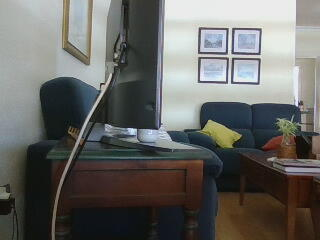
\includegraphics[width = 0.7\textwidth]{images/VideoRecibido6.1.png}
  \captionof{figure}{Vídeo recibido en \textit{Minimal\_Video} con latencia base de 250 ms.}
  \label{fig:minimal_video_250ms}
\end{center}

\newpage


Ahora, se ejecutará el módulo \textit{Minimal\_Video\_FPS} con una latencia base de 250 ms y el jitter severo asociado. El comando usado ha sido el siguiente:

\begin{lstlisting}[language=bash, basicstyle=\ttfamily\scriptsize]
    python minimal_video_fps.py -a 192.168.0.58 --show_video --show_stats -z 12
\end{lstlisting}
Donde \verb|-a| es la dirección IP destino, \verb|--show_video| es para que se active la transmisión de vídeo, \verb|--show_stats| es para que se muestre la información de estadísticas y \verb|-z| es el numero de fotogramas por segundo (FPS) que se desea enviar. En este caso, se ha configurado para mostrar el vídeo a 12 FPS.
\vspace{\baselineskip}

\begin{lstlisting}[language=bash,basicstyle=\ttfamily\tiny]
         |  AUDIO (msg)  |  VIDEO (msg)  |  AUDIO (kbps)   |  VIDEO (kbps)   |     CPU (%) 
   Cycle |  Sent  Recv   |  Sent  Recv   |   Sent   Recv   |   Sent   Recv   | Program System
================================================================================================
       1 |   31    28    |  165    93    |  1009    911    |  1833   1034    |  23      0       
       2 |   38    38    |    0     0    |  1232   1232    |     0      0    |  44     76       
       3 |   35    35    |  255   240    |  1143   1143    |  2846   2676    |  40     79       
       4 |   26    26    |  900   779    |   850    850    | 10050   8701    |  35     70       
       5 |   33    33    | 1341  1263    |  1065   1065    | 14783  13922    |  34     72       
       6 |   31    31    | 1464  1362    |   979    979    | 15787  14686    |  36     62       
       7 |   28    28    | 1143  1132    |   915    915    | 12762  12640    |  36     51       
       8 |   16    16    |  507   493    |   520    520    |  5625   5471    |  30     29       
       9 |   39    39    | 1247  1063    |  1277   1277    | 13941  11882    |  43     73       
      10 |   37    37    | 1192  1075    |  1211   1211    | 13325  12020    |  53     66       
      11 |   34    34    | 1519  1399    |  1068   1068    | 16297  15010    |  40     72       
      12 |   34    34    | 1761  1690    |  1086   1086    | 19212  18436    |  48     67       
      13 |    4     4    |  377   378    |   130    130    |  4200   4213    |   9     41       
   Cycle |  Sent  Recv   |  Sent  Recv   |   Sent   Recv   |   Sent   Recv   | Program System
         |  AUDIO (msg)  |  VIDEO (msg)  |  AUDIO (kbps)   |  VIDEO (kbps)   |     CPU (%) 
===========================================================================================
Video application stopped.

=== Global bandwidth statistics ===
Audio sent:       945.70 kbps
Audio received:   938.35 kbps
Video sent:       9929.23 kbps
Video received:   9173.34 kbps
Total time:       13.4 s
=====================================

=== FPS Statistics ===
Target FPS:       12.0
Average real FPS: 8.3
FPS efficiency:   69.1%
======================
Program terminated.
QObject::killTimer: Timers cannot be stopped from another thread
QObject::~QObject: Timers cannot be stopped from another thread
\end{lstlisting}

\newpage
La imagen de la Figura \ref{fig:minimal_video_fps_250ms} es una captura del vídeo recibido en esta prueba.
\begin{center}
  
\includegraphics[width = 0.7\textwidth]{images/VideoRecibido6.2.png}
  \captionof{figure}{Vídeo recibido en \textit{Minimal\_Video\_FPS} con latencia base de 250 ms.}
  \label{fig:minimal_video_fps_250ms}
\end{center}

\newpage


Ahora, se procederá a ejecutar el módulo \textit{Minimal\_Video\_Resolution} con una latencia base de 250 ms y el jitter severo asociado. El comando usado ha sido el siguiente:

\begin{lstlisting}[language=bash,basicstyle=\ttfamily\scriptsize]
python minimal_video_resolution.py -a 192.168.0.58 --show_video --show_stats -z 12 \\
-w 350 -g 250
\end{lstlisting}
Donde \verb|-a| indica la dirección IP destino, \verb|--show_video| indica que se active la transmisión de vídeo, \verb|--show_stats| indica que se muestren las estadísticas de la transmisión, \verb|-z| indica el número de fotogramas por segundo (FPS), \verb|-w| indica el ancho del vídeo y \verb|-g| indica la altura del vídeo.
\vspace{\baselineskip}

\begin{lstlisting}[language=bash,basicstyle=\ttfamily\tiny]
         |  AUDIO (msg)  |  VIDEO (msg)  |  AUDIO (kbps)   |  VIDEO (kbps)   |     CPU (%) 
   Cycle |  Sent  Recv   |  Sent  Recv   |   Sent   Recv   |   Sent   Recv   | Program System
================================================================================================
       1 |   27    27    |  188   188    |   883    883    |  2100   2100    |  22    100       
       2 |   31    26    |    0     0    |  1000    839    |     0      0    |  41     77       
       3 |   28    24    |  376   283    |   911    781    |  4178   3146    |  35     74       
       4 |   37    37    | 1245  1074    |  1190   1190    | 13670  11791    |  40     70       
       5 |   35    35    | 1032   816    |  1144   1144    | 11520   9110    |  43     66       
       6 |   33    33    | 1416  1291    |  1072   1072    | 15711  14323    |  40     71       
       7 |   29    29    | 1513  1430    |   948    948    | 16888  15963    |  31     68       
       8 |   35    35    | 1880  1791    |  1145   1145    | 21006  20013    |  46     71       
       9 |   17    17    | 1505  1463    |   551    551    | 16668  16205    |  39     70       
      10 |   38    38    |  713   453    |  1240   1240    |  7948   5049    |  46     61       
      11 |   28    28    |  965   850    |   915    915    | 10767   9485    |  36     67       
      12 |   33    33    | 1149  1006    |  1064   1064    | 12648  11072    |  36     72       
      13 |   13    13    |  919   858    |   424    424    | 10248   9567    |  17     70       
   Cycle |  Sent  Recv   |  Sent  Recv   |   Sent   Recv   |   Sent   Recv   | Program System
         |  AUDIO (msg)  |  VIDEO (msg)  |  AUDIO (kbps)   |  VIDEO (kbps)   |     CPU (%) 
===========================================================================================
Video application stopped.

=== Global bandwidth statistics ===
Audio sent:       932.17 kbps
Audio received:   910.32 kbps
Video sent:       10691.15 kbps
Video received:   9532.74 kbps
Total time:       13.5 s
=====================================

=== FPS Statistics ===
Target FPS:       12.0
Average real FPS: 6.0
FPS efficiency:   50.3%
======================

=== Resolution Statistics ===
Target resolution: 350x250
Actual resolution: 352x288
Average rescaling time: 6.43 ms
Performance impact:     7.7%
=============================

=== Camera compatible resolutions ===
  1. 320x240
  2. 352x288 * SELECTED
  3. 640x360
  4. 640x480
  5. 800x600
  6. 1024x768
  7. 1280x720
  8. 1280x1024
  9. 1366x768
  10. 1600x900
  11. 1920x1080
  12. 2560x1440
  13. 3840x2160

Camera device: /dev/video0
======================================
Program terminated.
QObject::killTimer: Timers cannot be stopped from another thread
QObject::~QObject: Timers cannot be stopped from another thread
\end{lstlisting}
\vspace{\baselineskip}

\newpage
La imagen de la Figura \ref{fig:minimal_video_resolution_250ms} es una captura del vídeo recibido en esta prueba.
\begin{center}
  
\includegraphics[width = 0.7\textwidth]{images/VideoRecibido6.3.png}
  \captionof{figure}{Vídeo recibido en \textit{Minimal\_Video\_Resolution} con latencia base de 250 ms.}
  \label{fig:minimal_video_resolution_250ms}
\end{center}
\newpage


Ahora, se procederá a analizar los resultados obtenidos en las pruebas realizadas con una latencia base de 250 ms y el jitter severo asociado.
\vspace{\baselineskip}

\textbf{Análisis de \textit{Minimal\_Video} con jitter alto y latencia de 250ms:}
\vspace{\baselineskip}

Al analizar el comportamiento de \textit{Minimal\_Video} bajo una latencia base de 250ms y el jitter severo, observamos un impacto notable pero no un colapso total. Las estadísticas globales muestran que el módulo envía audio a 956.82 kbps (recibiendo 929.90 kbps, un 97.2\%) y vídeo a 11274.19 kbps (recibiendo 10111.51 kbps, un 89.7\%). Estos porcentajes de recepción son bastante altos, indicando que la mayoría de los datos llegan al destino.
\vspace{\baselineskip}

Sin embargo, el análisis de los ciclos, especialmente el primero, muestra una recepción inicial de vídeo muy baja (89 kbps recibidos de 1836 kbps enviados), lo que refleja el impacto combinado de la alta latencia inicial y el jitter. Aunque los ciclos posteriores muestran una mejor recuperación en la cantidad de datos, la variabilidad asociada a un jitter severo y la alta latencia constante, perjudican significativamente la experiencia del usuario. La comunicación es percibida con un retraso considerable y una falta de fluidez debido a la llegada irregular de los paquetes, manifestándose en "tirones" y desincronizaciones.

\vspace{\baselineskip}

\textbf{Análisis de \textit{Minimal\_Video\_FPS} con jitter alto y latencia de 250ms:}
\vspace{\baselineskip}

Este módulo muestra una adaptación robusta al jitter severo y la alta latencia. Las estadísticas globales indican una transmisión de audio de 945.70 kbps (recibiendo 938.35 kbps, un 99.2\%) y de vídeo de 9929.23 kbps (recibiendo 9173.34 kbps, un 92.4\%). Estos porcentajes de recepción son excelentes, sugiriendo que el control de FPS ayuda a mitigar la pérdida de paquetes incluso en estas condiciones adversas.
\vspace{\baselineskip}

En cunato a las ``Estadísticas de FPS'' el módulo consigue mantener 8.3 FPS reales frente al objetivo de 12 FPS, alcanzando una eficiencia del 69.1\%. Para una latencia base tan alta y el jitter severo asociado, este es un rendimiento de FPS promedio muy bueno. Indica que el control de FPS se ajusta para enviar fotogramas a un ritmo que, aunque no ideal, es sostenible bajo estas condiciones extremas. Sin embargo, es importante entender que una media de 8.3 FPS bajo alto jitter no garantiza una visualización perfectamente fluida. La llegada de esos fotogramas será irregular, aunque la cantidad total transmitida sea alta. La experiencia del usuario estará marcada por el retardo de 250ms y una fluidez visual por la variabilidad en la entrega.

\vspace{\baselineskip}

\textbf{Análisis de \textit{Minimal\_Video\_Resolution} con jitter alto y latencia de 250ms:}
\vspace{\baselineskip}

Los resultados de este módulo bajo una latencia base de 250ms y jitter severo también son bastante positivos en términos de transmisión de datos y FPS promedio. Los datos globales muestran una transmisión de audio de 932.17 kbps (recibiendo 910.32 kbps, un 97.6\%) y de vídeo de 10691.15 kbps (recibiendo 9532.74 kbps, un 89.2\%).
\vspace{\baselineskip}

Las ``Estadísticas de FPS'' muestran un promedio de 6.0 FPS reales frente al objetivo de 12 FPS, alcanzando una eficiencia del 50.3\%. Aunque inferior al módulo \textit{Minimal\_Video\_FPS}, sigue siendo un resultado suficiente dadas las condiciones de red. El ``Tiempo de reescalado promedio'' de 6.43 ms (impacto del 7.7\%) es manejable. El módulo logra transmitir una cantidad significativa de datos y mantener una tasa de fotogramas promedio funcional. La combinación de control de FPS y ajuste de resolución parece ofrecer un buen compromiso para mantener la comunicación activa, aunque la fluidez está afectada por el alto jitter y la latencia.

\vspace{\baselineskip}

\textbf{Conclusiones para latencia base de 250ms con jitter alto:}

Una latencia base de 250ms, con el jitter severo asociado, establece condiciones muy difíciles, pero los módulos aguantan notablemente estas condiciones, especialmente en la cantidad de datos transmitidos y los FPS promedio:

\begin{itemize}
\item \textbf{Alta integridad de datos a pesar del jitter extremo:} Sorprendentemente, los tres módulos mantienen porcentajes de recepción de datos globales muy altos (audio >97\%, vídeo >89\%), lo que indica que la pérdida de paquetes no es el factor dominante, sino la irregularidad en su llegada.
\item \textbf{Rendimiento de FPS notable bajo condiciones adversas:} \textit{Minimal\_Video\_FPS} destaca con una eficiencia del 69.1\% (8.3 FPS reales), seguido de \textit{Minimal\_Video\_Resolution} con 50.3\% (6.0 FPS reales). Estos valores sugieren que los mecanismos de control de FPS se adaptan para mantener una tasa de envío viable incluso con un jitter muy elevado.
\item \textbf{Impacto de la latencia y el jitter en la experiencia del usuario:} Aunque se transmiten muchos datos y se logran FPS promedio considerables, la experiencia del usuario estará severamente degradada por el retraso de 250ms y la llegada errática de los fotogramas, causando una sensación de desconexión y falta de fluidez.
\item \textbf{Adaptabilidad de los módulos con control de FPS:} Los módulos \textit{Minimal\_Video\_FPS} y \textit{Minimal\_Video\_Resolution} muestran una capacidad significativa para ajustarse a un entorno de red muy adverso, priorizando mantener un flujo de fotogramas.
\item \textbf{El problema de la irregularidad:} Bajo estas condiciones, el principal problema para la calidad de la videollamada no es tanto la pérdida de paquetes (que es baja), sino la enorme variabilidad en los tiempos de llegada, lo que hace imposible una reproducción fluida y sincronizada sin mecanismos de buffering muy sofisticados y tolerantes a grandes retrasos.
\end{itemize}

Estos resultados demuestran que, si bien una latencia base alta y un jitter severo perjudican gravemente la calidad percibida de una videollamada, los módulos pueden seguir transmitiendo una cantidad considerable de datos y mantener una tasa de fotogramas promedio funcional. La clave está en la irregularidad de la entrega, que es el principal obstáculo para una experiencia de usuario satisfactoria.
\newpage

\subsubsection{Experimentos con pérdida de paquetes}

Ahora, se procederá a analizar los resultados obtenidos en las pruebas realizadas con pérdida de paquetes. 
\vspace{\baselineskip}
\begin{itemize}
  \item \textbf{Pruebas frente a pérdida de paquetes}
\end{itemize}

\textbf{Pruebas frente a pérdida de paquetes del 5\%:}
\vspace{\baselineskip}

Comenzaremos con una pérdida del 5\% de paquetes. El comando usado en \textit{Minimal\_Video} ha sido el siguiente:

\begin{lstlisting}[language=bash]
python minimal_video.py -a 192.168.0.58 --show_video --show_stats
\end{lstlisting}
Donde \verb|-a| es la dirección IP del dispositivo con el que se va a comunicar el módulo, \verb|--show_video| es la opción para mostrar el vídeo en tiempo real y \verb|--show_stats| es la opción para mostrar las estadísticas de la red.
\vspace{\baselineskip}

\begin{lstlisting}[language=bash,basicstyle=\ttfamily\tiny]
         |  AUDIO (msg)  |  VIDEO (msg)  |  AUDIO (kbps)   |  VIDEO (kbps)   |     CPU (%) 
   Cycle |  Sent  Recv   |  Sent  Recv   |   Sent   Recv   |   Sent   Recv   | Program System
================================================================================================
       1 |   23    23    |  165   150    |   748    748    |  1834   1669    |  30      0       
       2 |   37    37    |    0     0    |  1210   1210    |     0      0    |  52     78       
       3 |   33    33    |    0     0    |  1067   1067    |     0      0    |  51     76       
       4 |   25    25    |  252   252    |   815    815    |  2805   2801    |  29     77       
       5 |   30    30    |  971   933    |   980    980    | 10839  10416    |  25     76       
       6 |   30    30    | 1086  1067    |   981    981    | 12125  11914    |  36     78       
       7 |   35    27    |  472   220    |  1134    875    |  5225   2433    |  32     69       
       8 |   27    18    |  953   868    |   875    583    | 10544   9604    |  31     73       
       9 |   33    33    |  763   741    |  1078   1078    |  8510   8264    |  36     73       
      10 |   32    32    |  883   846    |  1036   1036    |  9764   9354    |  35     70       
      11 |   40    40    |  916   873    |  1307   1307    | 10224   9743    |  32     76       
      12 |   35    35    |  814   788    |  1138   1138    |  9039   8750    |  35     75       
      13 |   29    29    | 1226  1169    |   947    947    | 13673  13037    |  30     74       
      14 |    0     0    |   74    75    |     0      0    |   825    836    |   0     42       
   Cycle |  Sent  Recv   |  Sent  Recv   |   Sent   Recv   |   Sent   Recv   | Program System
         |  AUDIO (msg)  |  VIDEO (msg)  |  AUDIO (kbps)   |  VIDEO (kbps)   |     CPU (%) 
===========================================================================================
Video application stopped.

=== Global bandwidth statistics ===
Audio sent:       937.22 kbps
Audio received:   898.27 kbps
Video sent:       6708.33 kbps
Video received:   6244.18 kbps
Total time:       14.3 s
=====================================
Program terminated.
QObject::killTimer: Timers cannot be stopped from another thread
QObject::~QObject: Timers cannot be stopped from another thread
\end{lstlisting}
\vspace{\baselineskip}

\newpage

La imagen de la Figura \ref{fig:minimal_video_5percent} es una captura del vídeo recibido en esta prueba.
\begin{center}
  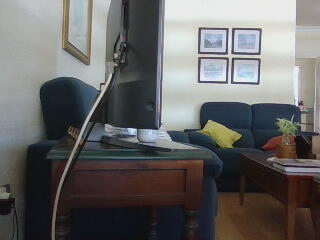
\includegraphics[width = 0.7\textwidth]{images/VideoRecibido7.1.png}
  \captionof{figure}{Vídeo recibido en \textit{Minimal\_Video} con una pérdida del 5\% de paquetes.}
  \label{fig:minimal_video_5percent}
\end{center}
\newpage


Ahora, se ejecutará el módulo \textit{Minimal\_Video\_FPS} con una pérdida del 5\% de paquetes. El comando usado ha sido el siguiente:

\begin{lstlisting}[language=bash, basicstyle=\ttfamily\scriptsize]
    python minimal_video_fps.py -a 192.168.0.58 --show_video --show_stats -z 12
\end{lstlisting}
Donde \verb|-a| es la dirección IP destino, \verb|--show_video| es para que se active la transmisión de vídeo, \verb|--show_stats| es para que se muestre la información de estadísticas y \verb|-z| es el numero de fotogramas por segundo (FPS) que se desea enviar. En este caso, se ha configurado para mostrar el vídeo a 12 FPS.
\vspace{\baselineskip}

\begin{lstlisting}[language=bash,basicstyle=\ttfamily\tiny]
         |  AUDIO (msg)  |  VIDEO (msg)  |  AUDIO (kbps)   |  VIDEO (kbps)   |     CPU (%) 
   Cycle |  Sent  Recv   |  Sent  Recv   |   Sent   Recv   |   Sent   Recv   | Program System
================================================================================================
       1 |   25    25    |  165   157    |   814    814    |  1834   1747    |  30      0       
       2 |   39    39    |    0     0    |  1252   1252    |     0      0    |  31     80       
       3 |    7     7    |   17    17    |   208    208    |   173    173    |  30     28       
       4 |   22    22    |  706   697    |   705    705    |  7731   7634    |  27     77       
       5 |   35    35    | 1296  1254    |  1141   1141    | 14430  13964    |  55     72       
       6 |   24    24    |  948   898    |   784    784    | 10580  10023    |  31     77       
       7 |   28    28    |  953   915    |   913    913    | 10612  10186    |  33     80       
       8 |   29    29    |  995   942    |   949    949    | 11116  10523    |  43     75       
       9 |   26    26    | 1316  1250    |   851    851    | 14708  13969    |  31     76       
      10 |   33    33    | 1051   968    |  1050   1050    | 11415  10515    |  38     75       
      11 |   37    37    | 1088  1034    |  1164   1164    | 11691  11110    |  59     80       
      12 |   25    25    |  803   791    |   789    789    |  8655   8526    |  37     81       
      13 |   39    39    |  703   638    |  1269   1269    |  7813   7092    |  36     75       
      14 |    0     0    |  165   163    |     0      0    |  1843   1821    |   2     45       
   Cycle |  Sent  Recv   |  Sent  Recv   |   Sent   Recv   |   Sent   Recv   | Program System
         |  AUDIO (msg)  |  VIDEO (msg)  |  AUDIO (kbps)   |  VIDEO (kbps)   |     CPU (%) 
===========================================================================================
Video application stopped.

=== Global bandwidth statistics ===
Audio sent:       833.44 kbps
Audio received:   833.44 kbps
Video sent:       7869.79 kbps
Video received:   7498.43 kbps
Total time:       14.5 s
=====================================

=== FPS Statistics ===
Target FPS:       12.0
Average real FPS: 5.7
FPS efficiency:   47.3%
======================
Program terminated.
QObject::killTimer: Timers cannot be stopped from another thread
QObject::~QObject: Timers cannot be stopped from another thread
\end{lstlisting}
\vspace{\baselineskip}

\newpage
La imagen de la Figura \ref{fig:minimal_video_fps_5percent} es una captura del vídeo recibido en esta prueba.
\begin{center}
  
\includegraphics[width = 0.7\textwidth]{images/VideoRecibido7.2.png}
  \captionof{figure}{Vídeo recibido en \textit{Minimal\_Video\_FPS} con una pérdida del 5\% de paquetes.}
  \label{fig:minimal_video_fps_5percent}
\end{center}
\newpage


Ahora, se procederá a ejecutar el módulo \textit{Minimal\_Video\_Resolution} con una pérdida del 5\% de paquetes. El comando usado ha sido el siguiente:

\begin{lstlisting}[language=bash,basicstyle=\ttfamily\scriptsize]
python minimal_video_resolution.py -a 192.168.0.58 --show_video --show_stats -z 12 \\
-w 350 -g 250
\end{lstlisting}
Donde \verb|-a| indica la dirección IP destino, \verb|--show_video| indica que se active la transmisión de vídeo, \verb|--show_stats| indica que se muestren las estadísticas de la transmisión, \verb|-z| indica el número de fotogramas por segundo (FPS), \verb|-w| indica el ancho del vídeo y \verb|-g| indica la altura del vídeo.
\vspace{\baselineskip}

\begin{lstlisting}[language=bash,basicstyle=\ttfamily\tiny]
         |  AUDIO (msg)  |  VIDEO (msg)  |  AUDIO (kbps)   |  VIDEO (kbps)   |     CPU (%) 
   Cycle |  Sent  Recv   |  Sent  Recv   |   Sent   Recv   |   Sent   Recv   | Program System
================================================================================================
       1 |   22    22    |  188   180    |   719    719    |  2100   2010    |  30      0       
       2 |   34    34    |    0     0    |  1107   1107    |     0      0    |  35     76       
       3 |   30    30    |    0     0    |   969    969    |     0      0    |  32     78       
       4 |   18    18    |  309   309    |   587    587    |  3442   3442    |  21     81       
       5 |   20    20    |  730   719    |   654    654    |  8152   8032    |  20     75       
       6 |   28    28    | 1307  1264    |   909    909    | 14485  14008    |  34     76       
       7 |   23    23    |  511   505    |   745    745    |  5657   5593    |  15     77       
       8 |   27    27    |  813   803    |   881    881    |  9060   8946    |  35     72       
       9 |   29    29    | 1010   998    |   949    949    | 11286  11151    |  19     76       
      10 |   35    35    |  604   594    |  1118   1118    |  6590   6483    |  43     75       
      11 |   37    37    | 1082  1038    |  1201   1201    | 12000  11511    |  30     73       
      12 |   32    32    | 1101  1059    |  1033   1033    | 12136  11673    |  34     73       
      13 |   33    33    |  933   890    |  1077   1077    | 10396   9917    |  32     75       
      14 |   20    20    |  808   788    |   653    653    |  9015   8794    |  24     69       
   Cycle |  Sent  Recv   |  Sent  Recv   |   Sent   Recv   |   Sent   Recv   | Program System
         |  AUDIO (msg)  |  VIDEO (msg)  |  AUDIO (kbps)   |  VIDEO (kbps)   |     CPU (%) 
===========================================================================================
Video application stopped.

=== Global bandwidth statistics ===
Audio sent:       877.27 kbps
Audio received:   877.27 kbps
Video sent:       7252.29 kbps
Video received:   7060.40 kbps
Total time:       14.5 s
=====================================

=== FPS Statistics ===
Target FPS:       12.0
Average real FPS: 5.0
FPS efficiency:   42.1%
======================

=== Resolution Statistics ===
Target resolution: 350x250
Actual resolution: 352x288
Average rescaling time: 5.30 ms
Performance impact:     6.4%
=============================

=== Camera compatible resolutions ===
  1. 320x240
  2. 352x288 * SELECTED
  3. 640x360
  4. 640x480
  5. 800x600
  6. 1024x768
  7. 1280x720
  8. 1280x1024
  9. 1366x768
  10. 1600x900
  11. 1920x1080
  12. 2560x1440
  13. 3840x2160

Camera device: /dev/video0
======================================
Program terminated.
QObject::killTimer: Timers cannot be stopped from another thread
QObject::~QObject: Timers cannot be stopped from another thread
\end{lstlisting}

\newpage
La imagen de la Figura \ref{fig:minimal_video_resolution_5percent} es una captura del vídeo recibido en esta prueba.
\begin{center}
  
\includegraphics[width = 0.7\textwidth]{images/VideoRecibido7.3.png}
  \captionof{figure}{Vídeo recibido en \textit{Minimal\_Video\_Resolution} con una pérdida del 5\% de paquetes.}
  \label{fig:minimal_video_resolution_5percent}
\end{center}

\newpage


Ahora, se procederá a analizar los resultados obtenidos en las pruebas realizadas con una pérdida del 5\% de paquetes.
\vspace{\baselineskip}

\textbf{Análisis de \textit{Minimal\_Video} con 5\% de pérdida de paquetes:}
\vspace{\baselineskip}

Al observar \textit{Minimal\_Video} bajo una pérdida del 5\% de paquetes, notamos un impacto directo en la cantidad de datos recibidos, como era de esperar. Las estadísticas globales muestran que el módulo envía audio a 937.22 kbps (recibiendo 898.27 kbps, lo que implica una pérdida efectiva en audio del 4.2\%) y vídeo a 6708.33 kbps (recibiendo 6244.18 kbps, una pérdida efectiva en vídeo del 6.9\%). Estos valores están alineados con la tasa de pérdida, aunque el vídeo parece ligeramente más afectado.
\vspace{\baselineskip}

El análisis por ciclos muestra fluctuaciones en la recepción, por ejemplo, en los ciclos 7 y 8, donde la recepción de audio y vídeo es notablemente inferior a la enviada. Esta variabilidad es característica de la pérdida de paquetes, que afecta de manera aleatoria pero continua a la transmisión. La experiencia del usuario se manifiesta en artefactos visuales (como bloques o congelaciones momentáneas cuando se pierden partes clave de un fotograma) y pequeños cortes en el audio.

\vspace{\baselineskip}

\textbf{Análisis de \textit{Minimal\_Video\_FPS} con 5\% de pérdida de paquetes:}
\vspace{\baselineskip}

Este módulo muestra una buena capacidad para mantener la integridad del audio frente a la pérdida de paquetes. Las estadísticas globales indican una transmisión de audio de 833.44 kbps (recibiendo el 100\% de este flujo), lo que es un resultado excelente para el audio. Para el vídeo, se enviaron 7869.79 kbps y se recibieron 7498.43 kbps, lo que representa una pérdida efectiva en vídeo del 4.7\%, muy cercana a la tasa de pérdida.
\vspace{\baselineskip}

Las ``Estadísticas de FPS'' muestran que el módulo logra 5.7 FPS reales frente al objetivo de 12 FPS, alcanzando una eficiencia del 47.3\%. Esta cifra indica que, aunque el módulo parece recibir bien el audio y la mayoría de los datos de vídeo que llegan, la pérdida de paquetes impacta la capacidad de mantener la tasa de fotogramas objetivo. El sistema probablemente reduce la tasa de envío o descarta fotogramas que no pueden ser reconstruidos completamente debido a la pérdida de paquetes para intentar mantener una calidad visual aceptable en los fotogramas que sí se muestran.

\vspace{\baselineskip}

\textbf{Análisis de \textit{Minimal\_Video\_Resolution} con 5\% de pérdida de paquetes:}
\vspace{\baselineskip}

Los datos globales de este módulo en esta prueba muestran una transmisión de audio de 877.27 kbps (recibiendo el 100\% de este flujo), lo que es, de nuevo, un resultado perfecto para el audio. Para el vídeo, se enviaron 7252.29 kbps y se recibieron 7060.40 kbps, lo que implica una pérdida efectiva en vídeo del 2.6\%. Este es el mejor resultado en términos de porcentaje de vídeo recibido entre los tres módulos bajo esta condición de pérdida.
\vspace{\baselineskip}

Las ``Estadísticas de FPS'' indican que el módulo alcanza 5.0 FPS reales frente al objetivo de 12 FPS, resultando en una eficiencia del 42.1\%. Aunque la pérdida de datos de vídeo es la más baja, la eficiencia de FPS es ligeramente inferior a la de \textit{Minimal\_Video\_FPS}. Esto podría sugerir que el módulo es más conservador al intentar reconstruir o mostrar fotogramas si falta alguna parte, priorizando la integridad del fotograma sobre la tasa. El ``Tiempo de reescalado promedio'' es de 5.30 ms, con un impacto en rendimiento del 6.4\%, valores razonables que indican que la limitación principal sigue siendo la pérdida de paquetes.

\vspace{\baselineskip}

\textbf{Conclusiones para pérdida de paquetes del 5\%:}

La prueba con una pérdida de paquetes moderada del 5\% revela cómo los diferentes módulos gestionan esta condición adversa:

\begin{itemize}
\item \textbf{Impacto directo en la recepción de vídeo:} \textit{Minimal\_Video} muestra una pérdida de datos tanto en audio (4.2\%) como en vídeo (6.9\%), en línea con lo esperado. Sin embargo, \textit{Minimal\_Video\_FPS} y \textit{Minimal\_Video\_Resolution} logran una recepción de audio del 100\% de lo enviado, y pérdidas de vídeo del 4.7\% y 2.6\% respectivamente. Esto sugiere que los mecanismos de control de FPS o la gestión de la transmisión en estos módulos podrían estar priorizando mejor el flujo de audio.
\item \textbf{Degradación de la eficiencia de FPS:} La pérdida de paquetes afecta significativamente la capacidad de alcanzar los 12 FPS objetivo. \textit{Minimal\_Video\_FPS} alcanza un 47.3\% de eficiencia (5.7 FPS reales) y \textit{Minimal\_Video\_Resolution} un 42.1\% (5.0 FPS reales). Aunque se transmiten muchos datos, la fluidez visual se ve comprometida.
\item \textbf{Variabilidad en la calidad de la transmisión:} El análisis por ciclos en \textit{Minimal\_Video} (ciclos 7 y 8) y la naturaleza de la pérdida de paquetes implican que la experiencia del usuario será inconsistente, con artefactos visuales e interrupciones de audio que aparecen de forma intermitente.
\item \textbf{Mecanismos de adaptación:} Los módulos con control de FPS parecen adaptarse a las pérdidas reduciendo la tasa de fotogramas efectiva para intentar asegurar que los fotogramas que se envían y reciben estén lo más completos posible, especialmente \textit{Minimal\_Video\_Resolution} que logra la menor tasa de pérdida de vídeo.
\end{itemize}

Estos resultados indican que una pérdida de paquetes del 5\% es un pequeño obstáculo para la comunicación en tiempo real. Aunque los módulos con control de FPS aguantan en la transmisión del audio y una pérdida de vídeo contenida, la fluidez se ve considerablemente afectada.
\newpage

\textbf{Pruebas frente a pérdida de paquetes del 25\%:}
\vspace{\baselineskip}

Ahora, realizaremos las pruebas con una pérdida del 25\% de paquetes. El comando usado en \textit{Minimal\_Video} ha sido el siguiente:

\begin{lstlisting}[language=bash]
python minimal_video.py -a 192.168.0.58 --show_video --show_stats
\end{lstlisting}
Donde \verb|-a| es la dirección IP del dispositivo con el que se va a comunicar el módulo, \verb|--show_video| es la opción para mostrar el vídeo en tiempo real y \verb|--show_stats| es la opción para mostrar las estadísticas de la red.
\vspace{\baselineskip}

\begin{lstlisting}[language=bash,basicstyle=\ttfamily\tiny]
         |  AUDIO (msg)  |  VIDEO (msg)  |  AUDIO (kbps)   |  VIDEO (kbps)   |     CPU (%) 
   Cycle |  Sent  Recv   |  Sent  Recv   |   Sent   Recv   |   Sent   Recv   | Program System
================================================================================================
       1 |   31     0    |  165    92    |  1003      0    |  1824   1018    |  36     75       
       2 |   40     3    |    0     0    |  1285     96    |     0      0    |  47     76       
       3 |   37    18    |  158    35    |  1203    585    |  1756    387    |  51     77       
       4 |   42    21    |  293     0    |  1355    677    |  3228      0    |  42     68       
       5 |   35    16    |  640   417    |  1143    522    |  7137   4654    |  37     68       
       6 |   31    17    |  477   329    |  1001    549    |  5258   3627    |  34     67       
       7 |   37    11    |  466   326    |  1202    357    |  5170   3617    |  51     71       
       8 |   27    16    |  372   262    |   877    520    |  4129   2907    |  26     69       
       9 |   23    20    |  425   314    |   738    642    |  4658   3444    |  35     72       
      10 |   37    13    |  499   305    |  1209    424    |  5568   3403    |  38     72       
      11 |   36    19    |  497   327    |  1177    621    |  5549   3651    |  33     72       
      12 |   26    20    |  483   356    |   850    654    |  5395   3979    |  32     69       
      13 |    9     6    |  303   212    |   288    192    |  3311   2317    |  14     42       
   Cycle |  Sent  Recv   |  Sent  Recv   |   Sent   Recv   |   Sent   Recv   | Program System
         |  AUDIO (msg)  |  VIDEO (msg)  |  AUDIO (kbps)   |  VIDEO (kbps)   |     CPU (%) 
===========================================================================================
Video application stopped.

=== Global bandwidth statistics ===
Audio sent:       1002.06 kbps
Audio received:   438.86 kbps
Video sent:       3977.00 kbps
Video received:   2476.75 kbps
Total time:       13.4 s
=====================================
Program terminated.
QObject::killTimer: Timers cannot be stopped from another thread
QObject::~QObject: Timers cannot be stopped from another thread
\end{lstlisting}
\vspace{\baselineskip}

\newpage
La imagen de la Figura \ref{fig:minimal_video_25percent} es una captura del vídeo recibido en esta prueba.
\begin{center}
  
\includegraphics[width = 0.7\textwidth]{images/VideoRecibido8.1.png}
  \captionof{figure}{Vídeo recibido en \textit{Minimal\_Video} con una pérdida del 25\% de paquetes.}
  \label{fig:minimal_video_25percent}
\end{center}

\newpage


Ahora, se ejecutará el módulo \textit{Minimal\_Video\_FPS} con una pérdida del 25\% de paquetes. El comando usado ha sido el siguiente:

\begin{lstlisting}[language=bash, basicstyle=\ttfamily\scriptsize]
    python minimal_video_fps.py -a 192.168.0.58 --show_video --show_stats -z 12
\end{lstlisting}
Donde \verb|-a| es la dirección IP destino, \verb|--show_video| es para que se active la transmisión de vídeo, \verb|--show_stats| es para que se muestre la información de estadísticas y \verb|-z| es el numero de fotogramas por segundo (FPS) que se desea enviar. En este caso, se ha configurado para mostrar el vídeo a 12 FPS.
\vspace{\baselineskip}

\begin{lstlisting}[language=bash,basicstyle=\ttfamily\tiny]
         |  AUDIO (msg)  |  VIDEO (msg)  |  AUDIO (kbps)   |  VIDEO (kbps)   |     CPU (%) 
   Cycle |  Sent  Recv   |  Sent  Recv   |   Sent   Recv   |   Sent   Recv   | Program System
================================================================================================
       1 |   21    12    |  160   127    |   388    222    |  1012    802    |  42      0       
       2 |   21    21    |    5     4    |   591    591    |    46     38    |  10     84       
       3 |   38    31    |   66    65    |  1173    957    |   696    686    |  30     78       
       4 |   28    19    |  625   606    |   903    613    |  6885   6676    |  22     76       
       5 |   35    25    |  528   384    |  1133    809    |  5840   4247    |  37     70       
       6 |   24    18    |  431   319    |   784    588    |  4811   3561    |  36     71       
       7 |   31    13    |  347   254    |  1002    420    |  3832   2804    |  36     73       
       8 |   34    12    |  444   305    |  1094    386    |  4879   3350    |  50     75       
       9 |   35    19    |  492   353    |  1141    619    |  5479   3929    |  28     74       
      10 |   33     8    |  431   224    |  1080    261    |  4818   2503    |  25     71       
      11 |   38     5    |  466   351    |  1242    163    |  5199   3917    |  43     74       
      12 |   32     0    |  647   572    |  1043      0    |  7200   6364    |  29     73       
      13 |   13     0    |  460   374    |   424      0    |  5128   4168    |  10     65       
   Cycle |  Sent  Recv   |  Sent  Recv   |   Sent   Recv   |   Sent   Recv   | Program System
         |  AUDIO (msg)  |  VIDEO (msg)  |  AUDIO (kbps)   |  VIDEO (kbps)   |     CPU (%) 
===========================================================================================
Video application stopped.

=== Global bandwidth statistics ===
Audio sent:       877.05 kbps
Audio received:   419.06 kbps
Video sent:       3988.65 kbps
Video received:   3078.19 kbps
Total time:       14.3 s
=====================================

=== FPS Statistics ===
Target FPS:       12.0
Average real FPS: 3.0
FPS efficiency:   25.2%
======================
Program terminated.
QObject::killTimer: Timers cannot be stopped from another thread
QObject::~QObject: Timers cannot be stopped from another thread
\end{lstlisting}
\vspace{\baselineskip}

\newpage
La imagen de la Figura \ref{fig:minimal_video_fps_25percent} es una captura del vídeo recibido en esta prueba.
\begin{center}
  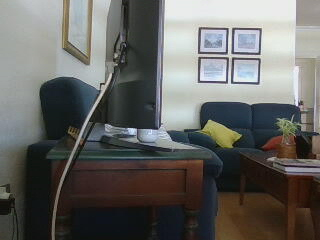
\includegraphics[width = 0.7\textwidth]{images/VideoRecibido8.2.png}
  \captionof{figure}{Vídeo recibido en \textit{Minimal\_Video\_FPS} con una pérdida del 25\% de paquetes.}
  \label{fig:minimal_video_fps_25percent}
\end{center}

\newpage


Ahora, se procederá a ejecutar el módulo \textit{Minimal\_Video\_Resolution} con una pérdida del 25\% de paquetes. El comando usado ha sido el siguiente:

\begin{lstlisting}[language=bash,basicstyle=\ttfamily\scriptsize]
python minimal_video_resolution.py -a 192.168.0.58 --show_video --show_stats -z 12 \\
-w 350 -g 250
\end{lstlisting}
Donde \verb|-a| indica la dirección IP destino, \verb|--show_video| indica que se active la transmisión de vídeo, \verb|--show_stats| indica que se muestren las estadísticas de la transmisión, \verb|-z| indica el número de fotogramas por segundo (FPS), \verb|-w| indica el ancho del vídeo y \verb|-g| indica la altura del vídeo.
\vspace{\baselineskip}

\begin{lstlisting}[language=bash,basicstyle=\ttfamily\tiny]
         |  AUDIO (msg)  |  VIDEO (msg)  |  AUDIO (kbps)   |  VIDEO (kbps)   |     CPU (%) 
   Cycle |  Sent  Recv   |  Sent  Recv   |   Sent   Recv   |   Sent   Recv   | Program System
================================================================================================
       1 |   23    20    |  188   187    |   751    653    |  2097   2086    |  22      0       
       2 |   37    19    |    0     0    |  1210    621    |     0      0    |  34     80       
       3 |   22     8    |  259   259    |   711    258    |  2861   2856    |  33     79       
       4 |   27    16    |  601   521    |   858    508    |  6522   5653    |  23     76       
       5 |   32    25    |  409   320    |  1047    818    |  4570   3574    |  33     72       
       6 |   37    12    |  592   415    |  1206    391    |  6591   4623    |  39     71       
       7 |   36    18    |  529   373    |  1169    584    |  5867   4137    |  41     71       
       8 |   34    20    |  528   390    |  1098    646    |  5824   4300    |  41     71       
       9 |   33    20    |  532   377    |  1059    641    |  5827   4132    |  43     71       
      10 |   38    23    |  487   345    |  1241    751    |  5433   3845    |  37     77       
      11 |   39    12    |  513   336    |  1275    392    |  5727   3756    |  36     72       
      12 |   33     8    |  440   265    |  1078    261    |  4906   2954    |  32     72       
      13 |    0     0    |  178   130    |     0      0    |  1988   1451    |   3     46       
   Cycle |  Sent  Recv   |  Sent  Recv   |   Sent   Recv   |   Sent   Recv   | Program System
         |  AUDIO (msg)  |  VIDEO (msg)  |  AUDIO (kbps)   |  VIDEO (kbps)   |     CPU (%) 
===========================================================================================
Video application stopped.

=== Global bandwidth statistics ===
Audio sent:       948.40 kbps
Audio received:   487.54 kbps
Video sent:       4352.12 kbps
Video received:   3244.00 kbps
Total time:       13.5 s
=====================================

=== FPS Statistics ===
Target FPS:       12.0
Average real FPS: 2.1
FPS efficiency:   17.3%
======================

=== Resolution Statistics ===
Target resolution: 350x250
Actual resolution: 352x288
Average rescaling time: 3.98 ms
Performance impact:     4.8%
=============================

=== Camera compatible resolutions ===
  1. 320x240
  2. 352x288 * SELECTED
  3. 640x360
  4. 640x480
  5. 800x600
  6. 1024x768
  7. 1280x720
  8. 1280x1024
  9. 1366x768
  10. 1600x900
  11. 1920x1080
  12. 2560x1440
  13. 3840x2160

Camera device: /dev/video0
======================================
Program terminated.
QObject::killTimer: Timers cannot be stopped from another thread
QObject::~QObject: Timers cannot be stopped from another thread
\end{lstlisting}

\newpage

La imagen de la Figura \ref{fig:minimal_video_resolution_25percent} es una captura del vídeo recibido en esta prueba.
\begin{center}
  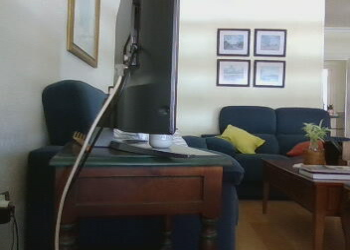
\includegraphics[width = 0.7\textwidth]{images/VideoRecibido8.3.png}
  \captionof{figure}{Vídeo recibido en \textit{Minimal\_Video\_Resolution} con una pérdida del 25\% de paquetes.}
  \label{fig:minimal_video_resolution_25percent}
\end{center}

\newpage

Ahora, se procederá a analizar los resultados obtenidos en las pruebas realizadas con una pérdida del 25\% de paquetes.
\vspace{\baselineskip}

\textbf{Análisis de \textit{Minimal\_Video} con 25\% de pérdida de paquetes:}
\vspace{\baselineskip}

El impacto de una pérdida de paquetes del 25\% en \textit{Minimal\_Video} es severo y hace que la comunicación sea muy deficiente. Las estadísticas globales revelan que el módulo envía audio a 1002.06 kbps pero recibe solo 438.86 kbps (una pérdida efectiva de audio del 56.2\%), mientras que para vídeo envía 3977.00 kbps y recibe 2476.75 kbps (una pérdida efectiva de vídeo del 37.7\%). La pérdida real observada, especialmente en el audio, es significativamente mayor que el 25\%, lo que sugiere que la pérdida de ciertos paquetes tiene un efecto en cascada, comprometiendo la recepción de otros paquetes dependientes o fragmentos de mensajes.
\vspace{\baselineskip}

El análisis por ciclos muestra un comportamiento errático. Por ejemplo, en el ciclo 1, la recepción de audio es nula, y en el ciclo 4, la recepción de vídeo es nula. A lo largo de la prueba, la cantidad de mensajes de audio y vídeo recibidos es baja en comparación con los enviados. Esta inconsistencia provoca una experiencia de usuario fragmentada, con constantes y largas interrupciones tanto en el audio como en el vídeo. La comunicación se vuelve prácticamente ininteligible y la visualización es realmente pobre.

\vspace{\baselineskip}

\textbf{Análisis de \textit{Minimal\_Video\_FPS} con 25\% de pérdida de paquetes:}
\vspace{\baselineskip}

Este módulo sufre igualmente un impacto devastador bajo una pérdida de paquetes tan elevada. Las estadísticas globales muestran una transmisión de audio de 877.05 kbps (recibiendo 419.06 kbps, una pérdida efectiva de audio del 52.2\%) y de vídeo de 3988.65 kbps (recibiendo 3078.19 kbps, una pérdida efectiva de vídeo del 22.8\%). Es interesante notar que, en este caso, la pérdida efectiva de vídeo está más cerca del 25\%, mientras que el audio sigue sufriendo una pérdida mucho mayor.
\vspace{\baselineskip}

Las ``Estadísticas de FPS'' muestran un dato crítico: el módulo solo alcanza 3.0 FPS reales frente al objetivo de 12 FPS, resultando en una eficiencia del 25.2\%. Esta tasa de fotogramas es extremadamente baja para una comunicación visual efectiva. El algoritmo de control de FPS, al detectar las pérdidas masivas, reduce drásticamente la frecuencia de envío o no puede reconstruir suficientes fotogramas. El resultado es una experiencia visual severamente degradada, con actualizaciones de imagen tan esporádicas que la percepción de movimiento es casi inexistente. Los últimos ciclos (12 y 13) muestran una recepción de audio nula.

\vspace{\baselineskip}

\textbf{Análisis de \textit{Minimal\_Video\_Resolution} con 25\% de pérdida de paquetes:}
\vspace{\baselineskip}

Este módulo, que combina control de FPS con resolución adaptada, también presenta un rendimiento muy pobre bajo condiciones de pérdida del 25\%. Los datos globales indican una transmisión de audio de 948.40 kbps (recibiendo 487.54 kbps, una pérdida efectiva de audio del 48.6\%) y de vídeo de 4352.12 kbps (recibiendo 3244.00 kbps, una pérdida efectiva de vídeo del 25.5\%). De nuevo, el audio es el más afectado.
\vspace{\baselineskip}

Las ``Estadísticas de FPS'' revelan un resultado crítico: apenas 2.1 FPS reales frente al objetivo de 12 FPS, con una eficiencia catastrófica del 17.3\%. En términos prácticos, esto significa una actualización de imagen cada casi medio segundo, lo que hace que la comunicación visual sea completamente inviable. El ``Tiempo de reescalado promedio'' es de 3.98 ms, con un impacto en rendimiento del 4.8\%; estos valores son bajos porque hay muy pocos fotogramas que procesar.
\vspace{\baselineskip}

\textbf{Conclusiones para pérdida de paquetes del 25\%:}

Una pérdida de paquetes del 25\% muestra un escenario extremo que degrada severamente la calidad de la comunicación, haciendo que los tres módulos sean prácticamente inutilizables para una videoconferencia:

\begin{itemize}
\item \textbf{Pérdida masiva en audio:} Los tres módulos experimentan pérdidas de audio efectivas entre el 48.6\% y el 56.2\%, muy superiores al 25\% de pérdida inducida. Esto hace que el audio sea intermitente e ininteligible.
\item \textbf{Tasas de FPS inutilizables:} Con FPS reales entre 2.1 y 3.0, la parte visual de la comunicación es una sucesión de imágenes estáticas con muy poca conexión entre ellas. La eficiencia de FPS oscila en niveles de entre 17.3\% y 25.2\%.
\item \textbf{Comunicación completamente fragmentada:} El análisis por ciclos muestra que la recepción de datos es errática y muy baja en muchos momentos, lo que se traduce en una experiencia de usuario con constantes cortes, congelaciones y pérdida de información.
\item \textbf{Impacto en la recepción de vídeo:} La pérdida efectiva de vídeo se sitúa entre el 22.8\% y el 37.7\%, lo que, combinado con los bajos FPS, resulta en una calidad visual pésima.
\item \textbf{Ineficacia de las funcionalidades avanzadas:} Las características como el control de FPS o el reescalado de resolución no pueden compensar un nivel de pérdida de paquetes tan alto. De hecho, \textit{Minimal\_Video\_Resolution} presenta la peor eficiencia de FPS.
\end{itemize}

Estos resultados muestran una pérdida de paquetes del 25\% que sobrepasa la capacidad de los módulos para ofrecer una comunicación mínimamente funcional. En estas condiciones de pérdida, se requerirían protocolos de transmisión mucho más robustos y tolerantes a errores o cambiar a modos de comunicación que demanden mucho menos ancho de banda y sean menos sensibles a la pérdida (como solo audio con códecs muy robustos). Para la videoconferencia tal como está implementada en estos módulos, este nivel de pérdida es insostenible.
\newpage

\textbf{Pruebas frente a pérdida de paquetes del 50\%}
\vspace{\baselineskip}

Finalmente, realizaremos la última prueba por una pérdida del 50\% de paquetes. El comando usado en \textit{Minimal\_Video} ha sido el siguiente:

\begin{lstlisting}[language=bash]
python minimal_video.py -a 192.168.0.58 --show_video --show_stats
\end{lstlisting}
Donde \verb|-a| es la dirección IP del dispositivo con el que se va a comunicar el módulo, \verb|--show_video| es la opción para mostrar el vídeo en tiempo real y \verb|--show_stats| es la opción para mostrar las estadísticas de la red.
\vspace{\baselineskip}

\begin{lstlisting}[language=bash,basicstyle=\ttfamily\tiny]
         |  AUDIO (msg)  |  VIDEO (msg)  |  AUDIO (kbps)   |  VIDEO (kbps)   |     CPU (%) 
   Cycle |  Sent  Recv   |  Sent  Recv   |   Sent   Recv   |   Sent   Recv   | Program System
================================================================================================
       1 |   29     8    |  165    78    |   929    256    |  1805    854    |  31    100       
       2 |   34     5    |    0     0    |  1056    155    |     0      0    |  47     74       
       3 |   35     5    |  262   182    |  1097    156    |  2804   1949    |  31     75       
       4 |   29     6    |  381   202    |   949    196    |  4260   2256    |  28     73       
       5 |   37     7    |  427   203    |  1210    228    |  4767   2267    |  25     70       
       6 |   39     4    |  412   219    |  1261    129    |  4547   2418    |  35     70       
       7 |   34     3    |  375   210    |  1107     97    |  4171   2334    |  39     67       
       8 |   29     7    |  383   215    |   940    226    |  4239   2377    |  35     67       
       9 |   35     4    |  416   180    |  1145    130    |  4645   2012    |  37     71       
      10 |   35     5    |  353   166    |  1145    163    |  3944   1854    |  34     72       
      11 |   25     8    |  393   193    |   818    261    |  4391   2158    |  35     66       
      12 |   11     4    |  223   114    |   360    130    |  2491   1275    |  16     42       
   Cycle |  Sent  Recv   |  Sent  Recv   |   Sent   Recv   |   Sent   Recv   | Program System
         |  AUDIO (msg)  |  VIDEO (msg)  |  AUDIO (kbps)   |  VIDEO (kbps)   |     CPU (%) 
===========================================================================================
Video application stopped.

=== Global bandwidth statistics ===
Audio sent:       984.90 kbps
Audio received:   174.74 kbps
Video sent:       3425.69 kbps
Video received:   1773.91 kbps
Total time:       12.4 s
=====================================
Program terminated.
QObject::killTimer: Timers cannot be stopped from another thread
QObject::~QObject: Timers cannot be stopped from another thread
\end{lstlisting}

\newpage
La imagen de la Figura \ref{fig:minimal_video_50percent} es una captura del vídeo recibido en esta prueba.
\begin{center}
  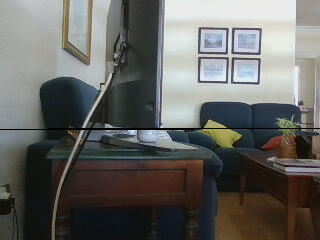
\includegraphics[width = 0.7\textwidth]{images/VideoRecibido9.1.png}
  \captionof{figure}{Vídeo recibido en \textit{Minimal\_Video} con una pérdida del 50\% de paquetes.}
  \label{fig:minimal_video_50percent}
\end{center}

\newpage


Ahora, se procederá a ejecutar el módulo \textit{Minimal\_Video\_FPS} con una pérdida del 50\% de paquetes. El comando usado ha sido el siguiente:

\begin{lstlisting}[language=bash, basicstyle=\ttfamily\scriptsize]
    python minimal_video_fps.py -a 192.168.0.58 --show_video --show_stats -z 12
\end{lstlisting}
Donde \verb|-a| es la dirección IP destino, \verb|--show_video| es para que se active la transmisión de vídeo, \verb|--show_stats| es para que se muestre la información de estadísticas y \verb|-z| es el numero de fotogramas por segundo (FPS) que se desea enviar. En este caso, se ha configurado para mostrar el vídeo a 12 FPS.
\vspace{\baselineskip}

\begin{lstlisting}[language=bash,basicstyle=\ttfamily\tiny]
         |  AUDIO (msg)  |  VIDEO (msg)  |  AUDIO (kbps)   |  VIDEO (kbps)   |     CPU (%) 
   Cycle |  Sent  Recv   |  Sent  Recv   |   Sent   Recv   |   Sent   Recv   | Program System
================================================================================================
       1 |   31     5    |  165    84    |  1007    162    |  1830    932    |  27      0       
       2 |   40     1    |    0     0    |  1304     32    |     0      0    |  46     75       
       3 |   35     3    |  148   125    |  1036     88    |  1498   1265    |  35     75       
       4 |   29     8    |  350   168    |   948    261    |  3904   1872    |  27     69       
       5 |   37     7    |  374   189    |  1190    225    |  4109   2074    |  45     65       
       6 |   37     7    |  338   155    |  1210    228    |  3774   1728    |  38     71       
       7 |   37     8    |  372   197    |  1197    258    |  4111   2179    |  45     74       
       8 |   38     7    |  423   207    |  1239    228    |  4707   2304    |  41     67       
       9 |   35     3    |  367   156    |  1145     98    |  4101   1741    |  43     67       
      10 |   30     8    |  324   181    |   978    261    |  3609   2018    |  48     66       
      11 |   36     0    |  342    30    |  1177      0    |  3818    335    |  53     72       
      12 |   24     8    |  396   216    |   782    260    |  4407   2406    |  37     69       
   Cycle |  Sent  Recv   |  Sent  Recv   |   Sent   Recv   |   Sent   Recv   | Program System
         |  AUDIO (msg)  |  VIDEO (msg)  |  AUDIO (kbps)   |  VIDEO (kbps)   |     CPU (%) 
===========================================================================================
Video application stopped.

=== Global bandwidth statistics ===
Audio sent:       1070.38 kbps
Audio received:   170.11 kbps
Video sent:       3215.71 kbps
Video received:   1526.27 kbps
Total time:       12.5 s
=====================================

=== FPS Statistics ===
Target FPS:       12.0
Average real FPS: 1.7
FPS efficiency:   14.0%
======================
Program terminated.
QObject::killTimer: Timers cannot be stopped from another thread
QObject::~QObject: Timers cannot be stopped from another thread
\end{lstlisting}

\newpage
La imagen de la Figura \ref{fig:minimal_video_fps_50percent} es una captura del vídeo recibido en esta prueba.
\begin{center}
  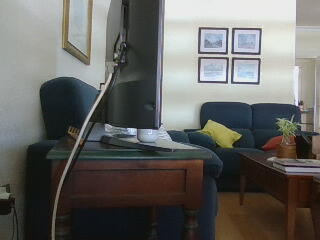
\includegraphics[width = 0.7\textwidth]{images/VideoRecibido9.2.png}
  \captionof{figure}{Vídeo recibido en \textit{Minimal\_Video\_FPS} con una pérdida del 50\% de paquetes.}
  \label{fig:minimal_video_fps_50percent}
\end{center}

\newpage


Ahora, se procederá a ejecutar el módulo \textit{Minimal\_Video\_Resolution} con una pérdida del 50\% de paquetes. El comando usado ha sido el siguiente:
\begin{lstlisting}[language=bash,basicstyle=\ttfamily\scriptsize]
python minimal_video_resolution.py -a 192.168.0.58 --show_video --show_stats -z 12 \\
-w 350 -g 250
\end{lstlisting}
Donde \verb|-a| indica la dirección IP destino, \verb|--show_video| indica que se active la transmisión de vídeo, \verb|--show_stats| indica que se muestren las estadísticas de la transmisión, \verb|-z| indica el número de fotogramas por segundo (FPS), \verb|-w| indica el ancho del vídeo y \verb|-g| indica la altura del vídeo.
\vspace{\baselineskip}

\begin{lstlisting}[language=bash,basicstyle=\ttfamily\tiny]
         |  AUDIO (msg)  |  VIDEO (msg)  |  AUDIO (kbps)   |  VIDEO (kbps)   |     CPU (%) 
   Cycle |  Sent  Recv   |  Sent  Recv   |   Sent   Recv   |   Sent   Recv   | Program System
================================================================================================
       1 |   20     4    |  165   104    |   646    129    |  1823   1146    |  20      0       
       2 |   35     4    |   23     0    |  1140    130    |   253      0    |  48     74       
       3 |   33     9    |    0     0    |  1079    294    |     0      0    |  63     74       
       4 |   31     4    |  346   321    |  1015    130    |  3870   3592    |  38     75       
       5 |   24     5    |  310   148    |   783    163    |  3453   1648    |  44     69       
       6 |   28     4    |  401   207    |   915    130    |  4475   2308    |  45     70       
       7 |   38     3    |  392   199    |  1242     98    |  4376   2224    |  57     72       
       8 |   33     2    |  420   176    |  1057     64    |  4593   1921    |  26     67       
       9 |   31     7    |  385   193    |  1013    228    |  4292   2155    |  24     70       
      10 |   35     5    |  400   184    |  1117    159    |  4360   2005    |  16     61       
      11 |   32     5    |  431   209    |  1035    161    |  4763   2312    |  15     63       
      12 |   35     3    |  399   189    |  1142     97    |  4447   2106    |  20     64       
      13 |    9     1    |  274   139    |   293     32    |  3051   1548    |  10     58       
   Cycle |  Sent  Recv   |  Sent  Recv   |   Sent   Recv   |   Sent   Recv   | Program System
         |  AUDIO (msg)  |  VIDEO (msg)  |  AUDIO (kbps)   |  VIDEO (kbps)   |     CPU (%) 
===========================================================================================
Video application stopped.

=== Global bandwidth statistics ===
Audio sent:       931.34 kbps
Audio received:   135.82 kbps
Video sent:       3267.15 kbps
Video received:   1713.44 kbps
Total time:       13.5 s
=====================================

=== FPS Statistics ===
Target FPS:       12.0
Average real FPS: 1.5
FPS efficiency:   12.7%
======================

=== Resolution Statistics ===
Target resolution: 350x250
Actual resolution: 352x288
Average rescaling time: 2.81 ms
Performance impact:     3.4%
=============================

=== Camera compatible resolutions ===
  1. 320x240
  2. 352x288 * SELECTED
  3. 640x360
  4. 640x480
  5. 800x600
  6. 1024x768
  7. 1280x720
  8. 1280x1024
  9. 1366x768
  10. 1600x900
  11. 1920x1080
  12. 2560x1440
  13. 3840x2160

Camera device: /dev/video0
======================================
Program terminated.
QObject::killTimer: Timers cannot be stopped from another thread
QObject::~QObject: Timers cannot be stopped from another thread
\end{lstlisting}

\newpage

La imagen de la Figura \ref{fig:minimal_video_resolution_50percent} es una captura del vídeo recibido en esta prueba.
\begin{center}
  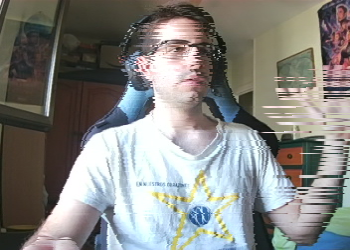
\includegraphics[width = 0.7\textwidth]{images/VideoRecibido9.3.png}
  \captionof{figure}{Vídeo recibido en \textit{Minimal\_Video\_Resolution} con una pérdida del 50\% de paquetes.}
  \label{fig:minimal_video_resolution_50percent}
\end{center}

\newpage

Ahora, se procederá a analizar los resultados obtenidos en las pruebas realizadas con una pérdida del 50\% de paquetes.
\vspace{\baselineskip}

\textbf{Análisis de \textit{Minimal\_Video} con 50\% de pérdida de paquetes:}
\vspace{\baselineskip}

El impacto de una pérdida de paquetes del 50\% en \textit{Minimal\_Video} es, como era de esperar, devastador para la comunicación. Las estadísticas globales muestran que el módulo envía audio a 984.90 kbps pero recibe solo 174.74 kbps (una pérdida efectiva de audio del 82.2\%), mientras que para vídeo envía 3425.69 kbps y recibe 1773.91 kbps (una pérdida efectiva de vídeo del 48.2\%). La pérdida real observada en el audio es drásticamente superior al 50\%, lo que indica que la pérdida de la mitad de los paquetes de audio hace que la mayor parte del flujo sea irrecuperable o ininteligible. La pérdida de vídeo está más cerca de la tasa de pérdida, pero sigue siendo masiva.
\vspace{\baselineskip}

El análisis por ciclos es muy grave, la cantidad de mensajes de audio recibidos es consistentemente una pequeña fracción de los enviados (por ejemplo, 4 de 39 en el ciclo 6, 3 de 34 en el ciclo 7). Aunque se recibe algo de vídeo, la cantidad es muy baja y la calidad es pésima. La comunicación es completamente inviable, con audio prácticamente ausente y un vídeo extremadamente fragmentado e incomprensible.

\vspace{\baselineskip}

\textbf{Análisis de \textit{Minimal\_Video\_FPS} con 50\% de pérdida de paquetes:}
\vspace{\baselineskip}

Este módulo también colapsa bajo una pérdida de paquetes del 50\%. Las estadísticas globales indican una transmisión de audio de 1070.38 kbps (recibiendo solo 170.11 kbps, una pérdida efectiva de audio del 84.1\%) y de vídeo de 3215.71 kbps (recibiendo 1526.27 kbps, una pérdida efectiva de vídeo del 52.5\%).
\vspace{\baselineskip}

Las ``Estadísticas de FPS'' muestran que el módulo apenas alcanza 1.7 FPS reales frente al objetivo de 12 FPS, resultando en una eficiencia del 14.0\%. Esto significa que se muestra menos de una imagen cada medio segundo, lo que hace imposible cualquier tipo de seguimiento visual. El control de FPS es incapaz de gestionar una pérdida tan masiva de información, y la comunicación visual es nula en la práctica. La recepción de audio también es mínima, como en el caso anterior.

\vspace{\baselineskip}

\textbf{Análisis de \textit{Minimal\_Video\_Resolution} con 50\% de pérdida de paquetes:}
\vspace{\baselineskip}

Finalmente, este módulo muestra resultados igualmente catastróficos, si no peores en el caso del audio. Los datos globales revelan una transmisión de audio de 931.34 kbps (recibiendo solo 135.82 kbps, una pérdida efectiva de audio del 85.4\%) y de vídeo de 3267.15 kbps (recibiendo 1713.44 kbps, una pérdida efectiva de vídeo del 47.6\%).
\vspace{\baselineskip}

Las ``Estadísticas de FPS'' muestran que el módulo apenas alcanza 1.5 FPS reales frente al objetivo de 12 FPS, con una eficiencia del 12.7\%. Este es el peor rendimiento de FPS de los tres módulos bajo esta condición. El ``Tiempo de reescalado promedio'' es de 2.81 ms, con un impacto en rendimiento del 3.4\%, pero estos datos son irrelevantes dado el colapso general de la comunicación. La combinación de reescalado y control de FPS no ofrece ninguna ventaja frente a una pérdida de paquetes tan extrema.
\vspace{\baselineskip}

\textbf{Conclusiones para pérdida de paquetes del 50\%:}

Una pérdida de paquetes del 50\% representa un escenario donde la comunicación audiovisual en tiempo real, con las implementaciones actuales de estos módulos, es imposible:
\vspace{\baselineskip}

\begin{itemize}
\item \textbf{Colapso de la transmisión de audio:} Los tres módulos experimentan pérdidas efectivas de audio superiores al 82\% (entre 82.2\% y 85.4\%). Esto resulta en un audio prácticamente inexistente, con solo fragmentos ininteligibles que llegan esporádicamente.
\item \textbf{FPS prácticamente inexistentes:} Con tasas de FPS reales entre 1.5 y 1.7, la componente visual de la comunicación se reduce a una presentación de imágenes extremadamente lenta y fragmentada. La eficiencia de FPS oscilan en niveles de entre el 12.7\% y el 14.0\%.
\item \textbf{Pérdida masiva de datos de vídeo:} Aunque la pérdida efectiva de vídeo (entre 47.6\% y 52.5\%) está más cerca del 50\% inducido que la del audio, sigue siendo una cantidad de información perdida tan grande que los fotogramas recibidos estarían severamente corruptos o incompletos.
\item \textbf{Inviabilidad de la comunicación:} La combinación de audio casi ausente y vídeo con FPS extremadamente bajos hace que cualquier intento de videoconferencia sea inútil. No se puede mantener una conversación ni seguir ninguna acción visual.
\end{itemize}

Estos resultados demuestran que una pérdida de paquetes del 50\% resulta en la imposibilidad de una comunicación audiovisual en tiempo real. Para una videoconferencia estándar, la comunicación es impracticable.
\newpage

% Reducir el espacio entre columnas para ganar más espacio para el texto
\setlength{\tabcolsep}{3pt} 

\begin{table} [htpb]
    \centering
    \renewcommand{\arraystretch}{1.25}
    \begin{tabularx}{\textwidth}{|>{\itshape\arraybackslash\scriptsize}p{3.2cm}|*{9}{>{\raggedright\arraybackslash\tiny}X|}}
    \hline
    & \multicolumn{3}{c|}{\textbf{\footnotesize Ancho de Banda Limitado}} & \multicolumn{3}{c|}{\textbf{\footnotesize Latencia (Delay)}} & \multicolumn{3}{c|}{\textbf{\footnotesize Pérdida de Paquetes}} \\
    \cline{2-10}
    \textbf{\footnotesize Módulo} & 
    \makecell[tc]{\textbf{\footnotesize 1 Mbps}} & \makecell[tc]{\textbf{\footnotesize 10 Mbps}} & \makecell[tc]{\textbf{\footnotesize 50 Mbps}} & 
    \makecell[tc]{\textbf{\footnotesize 0 ms}} & \makecell[tc]{\textbf{\footnotesize 100 ms}} & \makecell[tc]{\textbf{\footnotesize 250 ms}} & 
    \makecell[tc]{\textbf{\footnotesize 5\%}} & \makecell[tc]{\textbf{\footnotesize 25\%}} & \makecell[tc]{\textbf{\footnotesize 50\%}} \\
    \hline
    Minimal\_Video & 
    AT:954.02\newline AR:345.96\newline VT:1771.67\newline VR:762.21 &
    AT:860.65\newline AR:798.34\newline VT:5481.62\newline VR:4927.59 &
    AT:1000.25\newline AR:966.08\newline VT:8587.79\newline VR:7898.40 &
    AT:882.48\newline AR:799.36\newline VT:6587.96\newline VR:6353.34 &
    AT:962.34\newline AR:923.46\newline VT:11432.49\newline VR:10215.23 &
    AT:956.82\newline AR:929.90\newline VT:11274.19\newline VR:10111.51 &
    AT:937.22\newline AR:898.27\newline VT:6708.33\newline VR:6244.18 &
    AT:1002.06\newline AR:438.86\newline VT:3977.00\newline VR:2476.75 &
    AT:984.90\newline AR:174.74\newline VT:3425.69\newline VR:1773.91 \\
    \hline
    Minimal\_Video\_FPS & 
    AT:867.25\newline AR:391.50\newline VT:1862.96\newline VR:593.89\newline FPS~R:1.0\newline FPS~E:8.3\% &
    AT:980.18\newline AR:939.41\newline VT:2191.73\newline VR:1973.56\newline FPS~R:1.2\newline FPS~E:9.9\% &
    AT:976.67\newline AR:923.22\newline VT:8209.75\newline VR:7629.43\newline FPS~R:5.0\newline FPS~E:41.5\% &
    AT:955.12\newline AR:911.37\newline VT:7834.12\newline VR:7395.49\newline FPS~R:5.4\newline FPS~E:45.2\% &
    AT:936.37\newline AR:936.37\newline VT:13682.08\newline VR:13276.25\newline FPS~R:11.4\newline FPS~E:95.0\% &
    AT:945.70\newline AR:938.35\newline VT:9929.23\newline VR:9173.34\newline FPS~R:8.3\newline FPS~E:69.1\% &
    AT:833.44\newline AR:833.44\newline VT:7869.79\newline VR:7498.43\newline FPS~R:5.7\newline FPS~E:47.3\% &
    AT:877.05\newline AR:419.06\newline VT:3988.65\newline VR:3078.19\newline FPS~R:3.0\newline FPS~E:25.2\% &
    AT:1070.38\newline AR:170.11\newline VT:3215.71\newline VR:1526.27\newline FPS~R:1.7\newline FPS~E:14.0\% \\
    \hline
    Minimal\_Video\_Resolution & 
    AT:738.20\newline AR:360.10\newline VT:2311.06\newline VR:664.16\newline FPS~R:1.1\newline FPS~E:8.9\%\newline TR:6.47ms\newline IR:7.8\% &
    AT:546.99\newline AR:546.99\newline VT:3477.81\newline VR:3234.63\newline FPS~R:1.6\newline FPS~E:13.7\%\newline TR:6.47ms\newline IR:7.8\% &
    AT:904.14\newline AR:752.51\newline VT:7688.82\newline VR:6840.18\newline FPS~R:3.6\newline FPS~E:29.8\%\newline TR:5.53ms\newline IR:6.6\% &
    AT:933.82\newline AR:933.82\newline VT:7866.30\newline VR:7599.87\newline FPS~R:5.2\newline FPS~E:43.0\%\newline TR:3.06ms\newline IR:3.7\% &
    AT:896.90\newline AR:860.39\newline VT:12506.10\newline VR:11479.56\newline FPS~R:6.6\newline FPS~E:55.4\%\newline TR:5.67ms\newline IR:6.8\% &
    AT:932.17\newline AR:910.32\newline VT:10691.15\newline VR:9532.74\newline FPS~R:6.0\newline FPS~E:50.3\%\newline TR:6.43ms\newline IR:7.7\% &
    AT:877.27\newline AR:877.27\newline VT:7252.29\newline VR:7060.40\newline FPS~R:5.0\newline FPS~E:42.1\%\newline TR:5.30ms\newline IR:6.4\% &
    AT:948.40\newline AR:487.54\newline VT:4352.12\newline VR:3244.00\newline FPS~R:2.1\newline FPS~E:17.3\%\newline TR:3.98ms\newline IR:4.8\% &
    AT:931.34\newline AR:135.82\newline VT:3267.15\newline VR:1713.44\newline FPS~R:1.5\newline FPS~E:12.7\%\newline TR:2.81ms\newline IR:3.4\% \\
    \hline
    \multicolumn{10}{l}{\textit{\footnotesize AT: Audio Transmitido, AR: Audio Recibido, VT: Vídeo Transmitido, VR: Vídeo Recibido (kbps).}}\\
    \multicolumn{10}{l}{\textit{\footnotesize FPS R: FPS Real Promedio, FPS E: Eficiencia de FPS (\%). TR: Tiempo Reescalado (ms). IR: Impacto en Rendimiento (\%).}}
    \end{tabularx}
    \caption{Resumen de los experimentos realizados.}
    \label{tab:resumen_pruebas_globales}
\end{table}
\vspace{\baselineskip}

\newpage





\newpage
\section{Conclusión}
{\color{tfgazul}\rule{\textwidth}{3pt}}
\label{sec:conclusion}
En este capítulo se presentan las conclusiones obtenidas a partir de las pruebas realizadas con los módulos de videollamada desarrollados, que se resumen en la Tabla \ref{tab:resumen_pruebas_globales}. Estas pruebas abarcan diferentes condiciones de red, incluyendo variaciones en el ancho de banda, latencia, jitter y pérdida de paquetes. Los resultados obtenidos permiten evaluar el rendimiento y la adaptabilidad de cada módulo en situaciones diversas. Finalmente, se sugerirán posibles implementaciones futuras para mejorar el sistema existente y desarrollado en este trabajo.
\subsection{Conclusiones generales}
Las conclusiones que se pueden extraer de estas pruebas mostradas en la Tabla \ref{tab:resumen_pruebas_globales}, que abarcan diferentes condiciones y limitaciones de la red, son las siguientes:

\begin{itemize}
\item \textbf{Impacto del ancho de banda (capacidad de la red):}
\begin{itemize}
\item Con una capacidad muy baja (1 Mbps), la comunicación es prácticamente imposible. Se envía mucha más información de la que llega, especialmente el vídeo, y los fotogramas por segundo (FPS) son mínimos (solo 1 FPS, eficiencia del 8-9\%). La red está saturada.
\item Con una capacidad baja (10 Mbps), la situación mejora, pero sigue siendo difícil. Se recibe más información, pero los módulos que intentan ajustar los FPS todavía logran muy pocos (1.2-1.6 FPS, eficiencia del 9-14\%). La red aún se congestiona a veces.
\item Con una capacidad media (50 Mbps), la comunicación es buena. Se recibe casi toda la información enviada (más del 90\% del audio y vídeo). El módulo \textit{Minimal\_Video} funciona fluido. Los módulos que ajustan FPS mejoran bastante, logrando 5 FPS (\textit{Minimal\_Video\_FPS} con 41.5\% de eficiencia) y 3.6 FPS (\textit{Minimal\_Video\_Resolution} con 29.8\% de eficiencia), y la red no se satura.
\end{itemize}
\item \textbf{Efecto de la latencia (retraso en la red) y el jitter (variación del retraso):}
\begin{itemize}
    \item Con un retraso ideal (0 ms, jitter mínimo), la transmisión de datos es muy eficiente (llega más del 94\% del vídeo y más del 90\% del audio). Sin embargo, los módulos que ajustan FPS no alcanzan el objetivo de 12 FPS, quedándose en unos 5.2-5.4 FPS (eficiencia del 43-45\%), lo que indica que hay otros factores limitantes además de la red.
    \item Con un retraso moderado (100 ms y jitter asociado), sorprendentemente, el módulo \textit{Minimal\_Video\_FPS} alcanza su mejor rendimiento, llegando a 11.4 FPS (95\% de eficiencia). \textit{Minimal\_Video\_Resolution} también mejora a 6.6 FPS (55.4\% de eficiencia). La llegada de datos sigue siendo muy buena. Parece que este retraso ayuda a organizar mejor el envío de fotogramas.
    \item Con un retraso alto (250 ms y jitter severo), aunque la cantidad de datos que llega sigue siendo alta (más del 89\% del vídeo), la experiencia del usuario se ve afectada por el gran retraso y la irregularidad. Los módulos que ajustan FPS aún funcionan decentemente (8.3 FPS para \textit{Minimal\_Video\_FPS} y 6.0 FPS para \textit{Minimal\_Video\_Resolution}), pero la comunicación se siente poco fluida.
\end{itemize}

\item \textbf{Degradación por pérdida de paquetes:}
\begin{itemize}
    \item Con una pérdida baja (5\%), la comunicación es aceptable. El audio llega muy bien en los módulos con ajuste de FPS (casi el 100\% recibido), y la pérdida de vídeo es pequeña (llega el 93-97\%). Los FPS se mantienen sobre 5-5.7 (eficiencia del 42-47\%). Hay pequeños fallos visuales y de sonido.
    \item Con una pérdida media (25\%), la comunicación se degrada mucho. Se pierde casi la mitad del audio (llega solo el 44-51\%) y una cuarta parte del vídeo (llega el 62-77\%). Los FPS caen a 2-3 (eficiencia del 17-25\%), haciendo la videollamada prácticamente inútil.
    \item Con una pérdida muy alta (50\%), la comunicación colapsa. Se pierde la mayor parte del audio (llega solo el 15-18\%) y la mitad del vídeo (llega el 48-52\%). Los FPS son mínimos, entre 1.5 y 1.7 (eficiencia del 12-14\%), lo que es inviable.
\end{itemize}

\item \textbf{Adaptabilidad de los módulos:}
\begin{itemize}
    \item Los módulos \textit{Minimal\_Video\_FPS} y \textit{Minimal\_Video\_Resolution}, que intentan ajustar los FPS y la resolución, muestran un comportamiento interesante. Funcionan especialmente bien con retrasos moderados en la red (100 ms de latencia).
    \item Sin embargo, cuando la capacidad de la red es muy baja (1 Mbps) o la pérdida de paquetes es alta (25\% o más), estas funciones adaptativas no son suficientes para ofrecer una buena experiencia, y el rendimiento cae drásticamente, al igual que con el módulo básico.
    \item El proceso de cambiar la resolución en \textit{Minimal\_Video\_Resolution} (TR) es rápido (entre 2.8 y 6.5 milisegundos) y no consume muchos recursos del ordenador (impacto del 3-8\%), por lo que no es un problema en sí mismo.
\end{itemize}
\end{itemize}

Estas conclusiones indican que no hay un único módulo "mejor" para todas las situaciones.
El módulo \textbf{\textit{Minimal\_Video}} es sencillo y funciona bien si la red es buena (alta capacidad, bajo retraso y pocas pérdidas).
El módulo \textbf{\textit{Minimal\_Video\_FPS}} destaca por su capacidad de mantener una buena tasa de fotogramas cuando hay un retraso moderado en la red (como 100 ms).
El módulo \textbf{\textit{Minimal\_Video\_Resolution}} también se adapta bien al retraso y el cambio de resolución es eficiente.
En condiciones de red muy malas (capacidad de 1 Mbps o pérdidas de paquetes del 25\% o más), todos los módulos fallan en proporcionar una comunicación efectiva. La elección del módulo dependerá del tipo de problema de red que se espere encontrar.

\subsection{Trabajo futuro}
A partir del análisis de los resultados y las limitaciones observadas, en conjunto con todo lo expuesto en este proyecto, se proponen unas líneas y propuestas de trabajo a futuro para mejorar y expandir las capacidades del sistema de videollamada:

\begin{itemize}
\item \textbf{Mejorar la resistencia a la pérdida de paquetes:}
\begin{itemize}
\item \textbf{Corrección de errores hacia adelante (FEC):} Implementar técnicas como FEC, donde se envía información redundante junto con los datos originales. Esto permitiría al receptor reconstruir algunos paquetes perdidos sin necesidad de pedirlos de nuevo, mejorando la fluidez del vídeo y audio cuando la red pierde paquetes~\cite{fec}.
\end{itemize}
\item \textbf{Adaptación más inteligente al ancho de banda disponible:}
\begin{itemize}
    \item \textbf{Compresión de vídeo y audio más avanzada:} Aunque el proyecto se centra en módulos sin ningún tipo de compresión, la posible implementación de algoritmos de compresión de vídeo (como H.264, VP9)~\cite{h264} y audio (como Opus)~\cite{opus} podría reducir drásticamente la cantidad de datos necesarios, haciendo que la videollamada funcione mucho mejor con menos ancho de banda.
    \item \textbf{Ajuste dinámico de la calidad:} Desarrollar un sistema que mida continuamente la calidad de la red (ancho de banda, pérdida) y ajuste automáticamente la resolución del vídeo, los fotogramas por segundo (FPS) o el nivel de compresión para mantener la llamada lo más fluida posible. Por ejemplo, si la red empeora, podría reducir la calidad del vídeo para priorizar el audio.
\end{itemize}

\item \textbf{Optimización del rendimiento local para alcanzar los FPS deseados:}
\begin{itemize}
    \item \textbf{Revisión del proceso de captura y envío:} Investigar si hay cuellos de botella en el propio ordenador al capturar las imágenes de la cámara, procesarlas y enviarlas. Optimizar estas partes podría ayudar a alcanzar los FPS objetivo incluso cuando la red es buena.
\end{itemize}

\item \textbf{Mejor manejo del jitter:}
\begin{itemize}
    \item \textbf{Buffer de jitter adaptativo:} Implementar un pequeño buffer temporal en el lado del receptor que guarde los paquetes de audio y vídeo por un corto periodo antes de mostrarlos. Si este buffer ajusta su tamaño dinámicamente según la variación del retraso, puede ayudar a que el vídeo y el audio se reproduzcan de forma más continua, aunque los paquetes llegan de forma irregular.
\end{itemize}

\item \textbf{Nuevas funcionalidades y usabilidad:}
\begin{itemize}
    \item \textbf{Interfaz gráfica más completa:} Desarrollar una interfaz de usuario más amigable que permita configurar fácilmente las opciones.
    \item \textbf{Seguridad:} Añadir cifrado a la comunicación para proteger la privacidad de las conversaciones.
    \item \textbf{Servidor local:} Implementar un servidor local que gestione las conexiones y la comunicación entre los módulos con una interfaz web en la que se puedan ver los distintos dispositivos de la red y poder establecer comunicación entre ellos.
\end{itemize}
\end{itemize}

Estas mejoras podrían hacer que el sistema sea más robusto frente a diferentes condiciones de red y más fácil de usar, ofreciendo una experiencia de videollamada de mayor calidad en un rango más amplio de escenarios.

\newpage
\section{Bibliografía}
{\color{tfgazul}\rule{\textwidth}{3pt}}

% Bibliografía
\bibliographystyle{ieeetr}
\renewcommand{\refname}{} 
\bibliography{referencias}


\sinmarcaagua

\newpage
\begin{titlepage}
    \pagestyle{titlepage}
    \begin{tikzpicture}[remember picture, overlay]
        \node[inner sep=0pt] at (current page.center) {
            
\includegraphics[width=\paperwidth, height=\paperheight]{images/TFG_II_back}
        };
    \end{tikzpicture}
    
    % Título del grado en la parte inferior
    \begin{tikzpicture}[remember picture, overlay]
         \node[anchor=south east, inner sep=0pt] at ([xshift=-1.5cm, yshift=1.1cm]current page.south east) {
            \fontsize{16pt}{16pt}\selectfont \textbf{GRADO EN INGENIERÍA INFORMÁTICA  2024/2025}
         };
     \end{tikzpicture}
     
     % Resumen en el centro de la página
     \begin{tikzpicture}[remember picture, overlay]
         \node[anchor=center, inner sep=0pt, text width=0.6\paperwidth] at ([xshift=2.5cm, yshift=4cm]current page.center) {
            \fontfamily{ptm}\selectfont
\setlength{\parindent}{1.5em} % Sets paragraph indentation to 1.5em
\setlength{\parskip}{1.2em} % Space between paragraphs
\large

\begin{justify}
{\color{white}\noindent\hspace{1.5em}Este Trabajo Fin de Grado desarrolla diversos programas que complementan el ya existente ``InterCom'', un sistema de comunicación bidireccional que originalmente solo transmitía audio. El principal aporte de este proyecto ha sido implementar la capacidad de transmisión simultánea de vídeo junto con el audio, permitiendo una comunicación multimedia completa en tiempo real. El sistema desarrollado está diseñado para ser eficiente y funcionar en dispositivos con recursos limitados, ofreciendo distintas configuraciones de resolución compatibles con cada cámara y un control de la tasa de fotogramas por segundo (FPS).}

{\color{white}\noindent\hspace{1.5em}El trabajo ha consistido en desarrollar tres módulos principales: ``Minimal\_Video'' como base para la transmisión del vídeo, ``Minimal\_Video\_FPS'' para controlar la tasa de fotogramas por segundo según la resolución, y ``Minimal\_Video\_Resolution'' para reescalar la resolución en caso de incompatibilidad de la resolución solicitada por el usuario. Todo el código se ha implementado proporcionando una integración completa con el programa original ``InterCom'', enfocándose en minimizar la latencia y optimizar el uso de recursos de red, resultando en una herramienta académica que permite investigar y profundizar en las tecnologías de intercomunicación multimedia.}

{\color{white}\noindent\hspace{1.5em}Todo el código fue implementado en Python, manteniendo la compatibilidad con el subsistema de audio preexistente, y la documentación fue redactada utilizando LaTeX para garantizar una presentación profesional y estructurada del trabajo académico.}
\end{justify}
         };
     \end{tikzpicture}
    \thispagestyle{empty}
\end{titlepage}
\end{document}